% \usepackage{multirow}
% \usepackage{subcaption}
% \usepackage{tikz}
% \usepackage{pgfplots}
% \pgfplotsset{compat=newest}
% \pgfplotsset{plot coordinates/math parser=false}
% \newlength\fheight
% \newlength\fwidth
% \usetikzlibrary{plotmarks,decorations,backgrounds,calc,spy}
% \usetikzlibrary{decorations.markings}
% \usepgfplotslibrary{patchplots,groupplots}
% \usepackage{tikzscale}
% \usepackage{graphicx}

\newacronym{geo}{GEO}{Geostationary Equatorial Orbit}
\newacronym{meo}{MEO}{medium earth orbit}
\newacronym{leo}{LEO}{Low Earth Orbit}
\newacronym{vsat}{VSAT}{very small aperture terminal}
\newacronym{nb}{NB}{node base}
\newacronym{hap}{HAP}{High Altitute Platform}
\newacronym{mtc}{MTC}{machine type communications}
\newacronym{miot}{mIoT}{massive internet of things}
\newacronym{gcs}{GCS}{global coordinate system}
\newacronym{lcs}{LCS}{local coordinate system}
\newacronym{isl}{ISL}{inter-satellite link}
\newacronym{ecef}{ECEF}{Earth-Centered Earth-Fixed}
\newacronym{fspl}{FSPL}{free space path loss}
\newacronym{cnr}{CNR}{carrier-to-noise ratio}

\section{Introduction}
The large-scale deployment of cellular networks started at the end of last century.
Since then, the number of connected users has rapidly increased, together with the capabilities provided by wireless networks, now towards their \gls{6g}~\cite{giordani2020toward}.
This, together with the introduction of new applications in which millions or even billions of devices require connectivity services, such as \gls{iot} and \gls{v2x}, poses new challenges in terms of system capacity, network coverage, and service reliability. 
In this context, the research community is investigating the adoption of \glspl{ntn}~\cite{giordani2021non}, and the \gls{3gpp} has consolidated the possible use of \gls{ntn} into the \gls{nr} standard in Release~17~\cite{21917}.
In \gls{ntn}, \glspl{uav}, \glspl{hap}, and satellites can offer new connectivity opportunities, e.g., complementing already existing cellular systems, or providing broadband coverage to rural regions where it would otherwise be unfeasible to install cellular towers~\cite{Chaoub20216g}.
%Moreover, \gls{ntn} can act as centralized flying gateways to collect and process data faster than onboard terrestrial devices~\cite{wang2020potential,traspadini2023real}.

Satellites have been used from the 1990s to provide basic services such as phone and Internet access. Notably,  \gls{geo} satellites orbit at 35\,786 km, and offer global coverage at limited costs, despite the huge propagation delays. 
Only in the early 2010s the costs for satellite launch and maintenance have been low enough to allow for huge constellations of satellites to be launched in the \gls{leo}~\cite{satcost}. In particular, LEO provides wide coverage on the Earth, while promoting low~latency. 

Besides satellites, both \glspl{hap} and \glspl{uav} stand out as valid cost-effective alternatives for NTN. 
\glspl{uav}, flying at low altitudes (typically no more than 1 km), can guarantee on-demand support for ground networks, for example providing immediate assistance when cellular towers are overwhelmed or unavailable. \glspl{hap} operate in the stratosphere (from 20 to 50 km), and can be used to shape large coverage beams in  unpopulated areas, or provide services like backhauling and \gls{mec}, e.g., to gather and process data generated on the ground~\cite{traspadini2023real,wang2020potential}. %The assistance offered to the existing network infrastructure by \gls{hap} and \gls{uav} can play an important role in the public safety scenario, creating an additional communication channel for where an when needed, i.e. during large events. \glspl{hap} have shown to be an effective solution both when working as \gls{nb} as well as repeater on a bent-pipe architecture \cite{hapstwoways}.

Despite these premises, however, communication using space or airborne vehicles introduces new challenges compared to a terrestrial base station, including (i) severe \gls{pl} due to the longer propagation distance, (ii) additional attenuation from the atmosphere, such as scintillation, rain and clouds, (iii) Doppler shift due to the orbital mobility of satellites, and (iv) additional delays, mainly for propagation.
While experiments with real testbeds are impractical due to limitations in the scalability and flexibility of platforms, as well as the high cost of hardware components, the option to test network configurations via simulations on a sandbox environment facilitates the research process. Furthermore, an open-source simulator encourages research in the field, and offers industries and research institutions a better way to categorize and evaluate technologies. Among other simulators, ns-3 is a perfect open-source highly-customizable software to evaluate the end-to-end full-stack performance of networks~\cite{henderson2008network}.

%In this context, ns-3 offers full protocol stack and end-to-end implementations.
In this context, most simulators for \gls{ntn}, e.g., 5G K-Simulator \cite{5gksimulator}, 5GVienna~\cite{vienna5gsimulator}, or Simu5G \cite{simu5g}, are proprietary, or require some type of commercial license to use. Some others, while being open-source, sacrifice the accuracy of the higher layers to reduce the computational complexity, e.g., 5G-air-simulator \cite{5gairsimulator}. 

To fill these gaps, in this paper we present a new open-source module for ns-3 that implements the \gls{ntn} channel model based on the 3GPP specifications described in Technical Report 38.811~\cite{38811}.\footnote{The source code is publicly avaiable, and can be found at \cite{ntngitlab}.}
While our implementation is mainly related to the channel and the physical layer, a deep understanding of the propagation model is the first step towards proper protocol design~\cite{lecci2021accuracy}, which makes our module a valuable and accurate tool in the study of NTN.
Specifically, our module introduces: (i) new simulation scenarios for NTN; (ii) a new \gls{pl} model for the air/space channel in a wide range of frequencies (from 0.5 GHz to 100 GHz); (iii) the characterization of atmospheric absorptions; (iv) a new fast fading model for the space environment; (v) an antenna model for both terrestrial and non-terrestrial nodes; and (vi) a new coordinate system to account for the Geocentric Cartesian coordinate system of satellites. 

The rest of the paper is organized as follows. In Sec.~\ref{sec:channel} we describe the 3GPP channel for NTN, while our ns-3 implementation is reported in Sec.~\ref{sec:implementation}. In Sec.~\ref{sec:results-ntn} we validate the accuracy of our module against the 3GPP calibration results reported in 38.821~\cite{38821}. Then, we provide numerical results to measure the link-level and end-to-end performance as a function of different NTN parameters. Finally, Sec.~\ref{sec:conclusions} concludes the paper with suggestions for future research. 

%The implementation process is strictly related to the \gls{3gpp} recommendations for \gls{ntn} design, following the proposed procedures and methods, since they offer the state of the art regarding channel modeling, with parameters gathered in simulation campaigns in collaboration with industry leader organizations. All the created code undergoes a resource optimization analysis, being careful to use the appropriate data structures offered by C++ depending on the type of use and the size, staying coherent with the performance optimized ns-3. Furthermore, when a lack of guideline from \gls{3gpp} is found on certain matters and details, investigation in latest research findings is done to bring results as updated and as close to reality as possible.

\section{The 3GPP Channel Model for Non-Terrestrial Networks}
\label{sec:channel}
The channel model for \gls{ntn} has been formalized by the \gls{3gpp} in TR 38.811~\cite{38811}, and is based on the structure of the cellular channel model described in TR 38.901 \cite{TR38901}, already implemented in ns-3~\cite{zugno20implementation}. 
Following this rationale, in the following subsections we describe the \gls{ntn} channel model, including path loss, absorption, fading, and antenna models, as well as the coordinate system for satellites. 


\subsection{Scenarios and Path Loss Condition}
Similarly to the cellular channel model in \cite{TR38901}, the \gls{ntn} model gives the option to run simulations in four {scenarios}, to represent different propagation environments. Specifically:
\begin{itemize}
    \item Dense Urban: Extremely dense environment, with tall buildings acting as potential blockers.
    \item Urban: City environment, with buildings.
    \item Suburban: Small city, with up to two-storey buildings.
    \item Rural: Open field environment, with little or no buildings.
\end{itemize}
For satellites, only outdoor communication is possible, since attenuation from buildings would be enough to make the signal unusable. For \glspl{hap} or \glspl{uav}, instead, indoor communication is feasible, even though not yet implemented in our module. 

The 3GPP defines both \gls{los} and \gls{nlos} propagation, where the probability depends on the scenario and the elevation angle. The latter is defined as the angle between the horizon plane of the ground terminal and the vector pointing to the NTN platform. 

\subsection{Path Loss}
The basic path loss (in dB) can be written as
\begin{equation}
    PL_{b} = FSPL(d,f_{c})+SF+CL(\alpha,f_{c}).
    \label{eq:pl-fsp}
\end{equation}
The first term is the free space path loss, which can be calculated as
\begin{equation}
    FSPL(d,f_{c}) = 32.45 + 20log_{10}(f_{c}) + 20log_{10}(d),
\end{equation}
where $f_{c}$ is the carrier frequency in GHz and $d$ is the distance beteween the transmitter and the receiver in meters.
Notice that, while the channel model is valid for frequencies from 0.5 GHz to 100 GHz, two frequency bands are targeted in NTN, i.e., the S-band for frequencies below 6 GHz and the Ka-band for frequencies of 20 (30) GHz for downlink (uplink) transmissions, thereby in the millimeter-wave spectrum~\cite{giordani2020satellite}.

In Eq.~\eqref{eq:pl-fsp}, $SF$ represents the \gls{sf}, and is modeled as a log-normal random variable of zero mean and variance $\sigma_{SF}^2$, i.e., $SF \sim N\left ( 0,\sigma_{SF}^{2} \right )$. In order to calculate this variance, the model requires four parameters: the type of scenario, the frequency, the path loss condition (\gls{los} or \gls{nlos}), and the elevation angle. These parameters are used to find the correct entry in a table, given in~\cite{38811}.
A similar process is needed to calculate the clutter loss $CL(\alpha,f_{c})$.


\subsection{Atmospheric Absorption}
\label{sub:atm}
The attenuation introduced by the presence of atmospheric gasses was a marginal factor in the terrestrial channel.
%being left to calculation only in peculiar simulation. 
This is no longer the case for the \gls{ntn} channel, where atmospheric absorption plays a crucial role in the overall link budget. 
A complete and accurate characterization of the atmospheric attenuation is given in the ITU model~ \cite{itup676}, and depends on a set of parameters which is usually difficult to retrieve in simulations, such as absolute humidity, dry air pressure, water-vapour density and water-vapour partial pressure. 
Therefore, the \gls{3gpp} offers a simplified method considering only ground users placed at the sea level, with an elevation angle fixed to 90 degrees, and considering mean annual global values for the rest of the parameters. 
For elevation angles different than 90 degrees, the calculation is straightforward. Given the zenith attenuation $A_{zenith}(f_{c})$, the additional path loss due to atmospheric gasses is
\begin{equation}
    PL_{A,dB}\left ( \alpha,f_{c} \right )=\frac{A_{zenith}\left ( f_{c} \right ) }{sin(\alpha)},
\end{equation}
where $\alpha$ is the actual elevation angle.
Atmospheric absorption should be considered only for frequencies above 10 GHz, or for any frequency in case of $\alpha<10$ degrees.

\subsection{Scintillation}
Scintillation corresponds to the rapid fluctuation in amplitude and phase of the received signal, caused by the variation of the refractive index of the channel. 
Specifically, scintillation depends on location, time of the day, season, and solar and geomagnetic activity. Stronger levels of scintillation are observed only at high latitudes  (more than 60 degrees), in auroral and polar regions. 


While a complete absorption model would unnecessarily complicate system-level simulations, the 3GPP recommends a simplified model for scintillation~\cite{38811}, which is structured into two components: ionospheric scintillation and tropospheric scintillation.


\subsubsection{Ionospheric Scintillation}
Ionospheric scintillation is modeled based on the Gigahertz Scintillation Model~\cite{itup531}. While for the purpose of system–level simulations ionospheric scintillation is generally negligible at mid latitudes (between 20 and 60 degrees) or at above-6 GHz frequencies, in all other latitudes and conditions it is modeled as
\begin{equation}
    PL_{S,dB} = \left ( \frac{f_{c}}{4} \right )^{-1.5}\frac{P_{fluc}\left ( 4 \text{ GHz} \right )}{\sqrt{2}},
\end{equation}
where $f_{c}$ is the carrier frequency, and $P_{fluc}\left ( 4 \text{ GHz} \right )$ is a scaling factor representing the ionospheric attenuation level at 99\% of the time observed in Hong Kong between March 1977 and March 1978 at a frequency of 4 GHz~\cite[Fig.~6.6.6.1.4-1]{38811}.

\subsubsection{Tropospheric Scintillation}
Unlike ionospheric scintillation, the effect of tropospheric scintillation increases with the frequency, and becomes significant above 10 GHz. Furthermore, it increases at low elevation due to the longer path of the signal.  %\gls{3gpp} recommends considering the path loss induced by this effect only in certain cases, and offers a direct method for calculation. 
In these conditions, tropospheric scintillation is due to sudden changes in the refractive index due to the variation of temperature, water vapor content, and barometric pressure. For system-level simulations, the additional attenuation due to tropospheric scintillation is modeled as the attenuation level at 99\% of the time observed in Tolouse at 20 GHz, reported in~\cite[Fig.~6.6.6.2.1-1]{38811}. 

\subsection{Fast Fading}
As far as the fading is concerned, the 3GPP introduces both a flat-fading and a frequency-selective model. 
The flat-fading model, however, can be applied only if specific conditions are met, including (i) minimum elevation angle of 20 degrees, (ii) quasi-LOS propagation, (iii) communication in the S-band, (iv) channel bandwidth of at most 5 MHz, and (v) rural, suburban or urban scenario.
Hence, we consider the more general, though complex, frequency-selective fading model for \gls{ntn}. Then, the fading is based on the TR 38.901 model for cellular networks~\cite{TR38901} (already implemented in ns-3 in the \texttt{mmwave} module~\cite{zugno20implementation}), but with different parameters as described  in~\cite[Sec.~6.7.2]{38811}.

\subsection{Antenna Model}
Different antenna models are defined, depending on the device (satellite, HAP or UAV, and ground terminal). 
For satellites, the \gls{3gpp} suggests to use a circular aperture antenna model. Circular aperture antennas are reflector antennas that offer circular polarization. The normalized antenna gain pattern is given by
\begin{equation}
\label{eq:eq4}
    G(\theta) =
    \begin{cases}
    1  & \theta=0; \\
    4\left | \frac{J_{1}\left ( k\cdot \ell\cdot sin\theta \right )}{k\cdot \ell\cdot sin\theta} \right |^{2} & 0<\left | \theta \right |\leq 90^{\circ},
    \end{cases}
\end{equation}
where $J_{1}(\cdot)$ is the Bessel function of the first kind and first order, $\ell$ is the radius of the antenna's circular aperture and, given a carrier frequency  $f_{c}$, the value of $k$ is equal to $k={2\pi f_{c}}/{c}$, where $c$ is the speed of light in vacuum.

When considering flying vehicles that are not satellites, such as \glspl{hap} or \glspl{uav}, the lower distance makes it possible to use \gls{upa} antennas, that is the current standard for \glspl{ue} and eNB/gNB nodes in cellular networks according to the TR 38.901 model~\cite{TR38901}.

Finally, for terrestrial terminals, the 3GPP suggests to use either \gls{upa} antennas or \gls{vsat} antennas. The latter model, in particular, is a common choice in satellite communication, and consists of a circular reflector antenna of small size (less than 1 m of diameter), to be typically placed on roofs pointing at the sky. The \gls{vsat} radiation pattern is the same as that of circular aperture antennas for satellites, and is given in Eq.~\ref{eq:eq4}.

\subsection{Coordinate System}
\label{sec:coord_model}
In general, the 3GPP defines a simple Cartesian coordinate system where the position of each node is uniquely described by a set of three values, $(x,y,z)$, where $x$ and $y$ define the ground plane, and $z$ represents the height of the node. 
While this model is accurate enough to describe scenarios where nodes are deployed at close distance (e.g., a few hundreds of meters), it is not for scenarios where end nodes are placed hundred (or thousands) of kilometers apart such as in the NTN environment. In this case, the Earth's curvature, as well as the elevation angle, play an important role.
Therefore, the \gls{3gpp} suggests to use a Geocentric Cartesian coordinate system (or \gls{ecef} system), where the position of a node is still described by three values $(x,y,z)$, but now the origin of the axes lays in the center of the Earth, which is modeled as a sphere of radius $R=6\,371$ km. 
The x-y plane defines the equatorial plane, with the x-axis pointing at 0-degree longitude, the y-axis pointing at 90-degree longitude, and the z-axis pointing at the geographical North Pole. 
Then, terrestrial nodes on the surface of the Earth are deployed so that $\sqrt{x^{2}+y^{2}+z^{2}}=R$, while aerial/space nodes flying/orbiting around the Earth are deployed so that $\sqrt{x^{2}+y^{2}+z^{2}}> R$.


\section{Implementation}
\label{sec:implementation}
%The creation of the \gls{ntn} channel model follows the \gls{3gpp}~\cite{38811} guidelines presented in the previous section, which are considered a standard in the telecommunication landscape.  
The proposed ns-3 implementation of the 3GPP TR 38.811~\cite{38811} \gls{ntn} channel model is based upon the TR 38.901 model presented in~\cite{zugno20implementation}. Despite the fact that the newly introduced methods and classes are designed with the goal of introducing minimal changes to the existing ns-3 APIs, %, thus minimal change to existing classes is preferred.Nevertheless, 
some modifications to the existing code structure are still required. A schematic of these changes, which we make publicly available\footnote{\url{https://gitlab.com/mattiasandri/ns-3-ntn/-/tree/ntn-dev}}, can be found in Fig.~\ref{fig:ntn-uml}.

\begin{figure*}[t]
    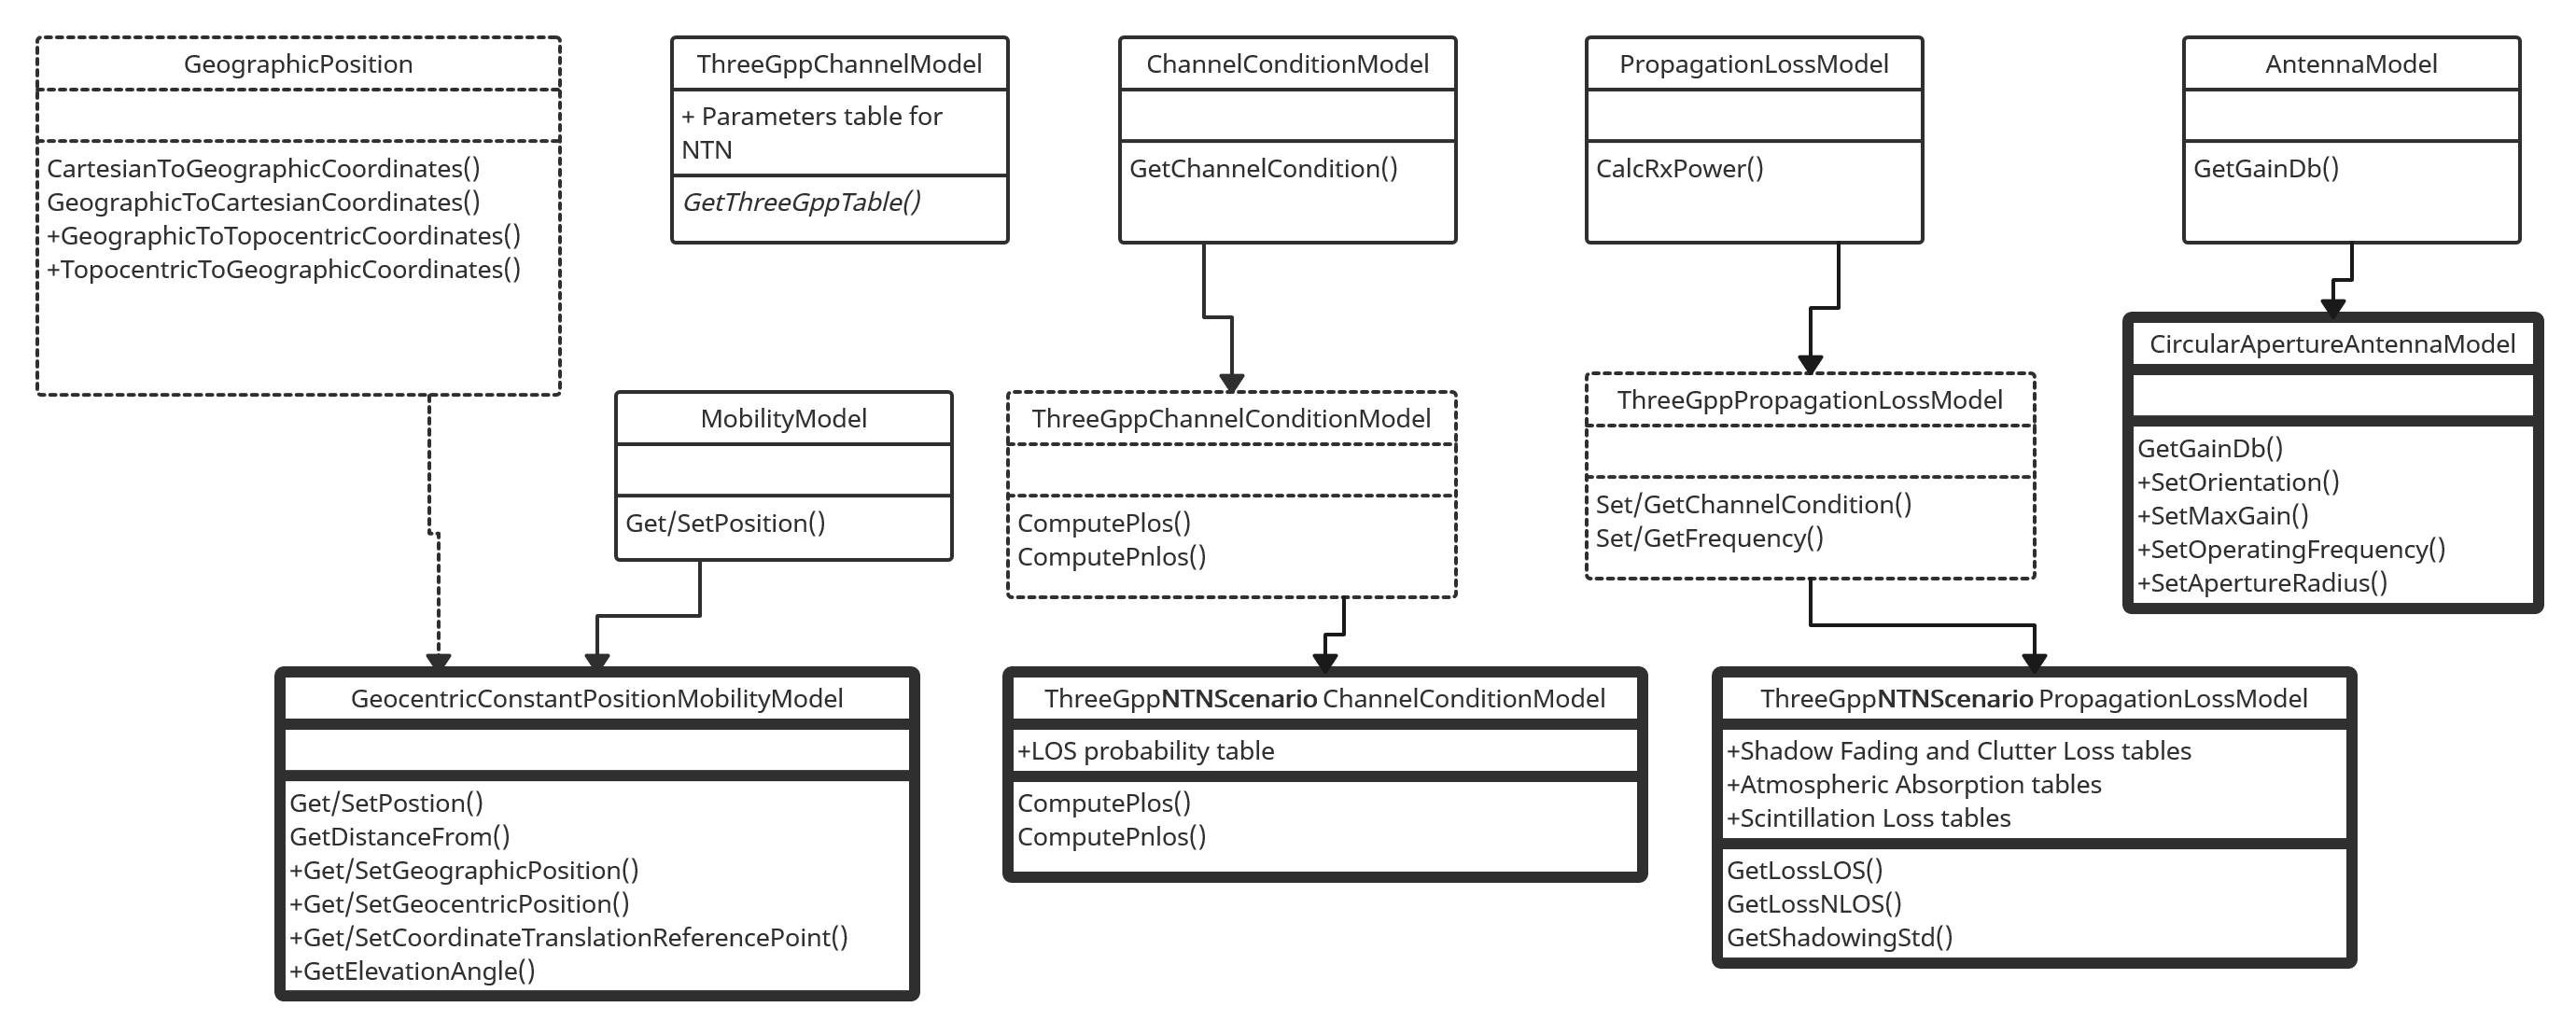
\includegraphics[width=\textwidth]{Figures/ChannelNtn/uml-diagram.png}
    \caption{Simplified UML diagram, which depicts the most significant changes which we introduced to ns-3. Bold classes represent the newly implemented ones, while dotted classes are pre-existing ones that have been modified.}
    \label{fig:ntn-uml}
\end{figure*}

The remainder of this section describes more in detail our implementation of the NTN channel model of~\cite{38811} in ns-3. 

%\subsection{ThreeGppChannelModel}
\subsection{Small-scale fading}
The most significant modifications to the pre-existing ns-3 classes concern the \texttt{Three\-Gpp\-Channel\-Model} class, which computes the small-scale propagation phenomena in the form of a complex channel matrix. Indeed, conversely from the procedure implemented in \cite{zugno20implementation}, in the \gls{ntn} channel model of~\cite{38811} most channel parameters depend on all the propagation scenario, \gls{los} condition, carrier frequency and elevation angle variables.  
To account for this, we store the small-scale fading parameters in a \emph{nested map}. The choice of this data-structure is motivated by the good trade-off between code efficiency and readability which it provides, considering that the possible combinations of the input parameters is particularly high, i.e., $144$.
%Taking into consideration four scenarios, two \gls{los} condition, two frequency band and nine elevation angle the final possible choices for a single parameters are 144. Given that the small scale parameters are more than 30 total values, a proper holding structure is needed to guarantee  bringing the choice to 

In particular, we change the signature of the \texttt{GetThreeGppTable()} method to include the \texttt{Mobility\-Model} instances of both transmitting and receiving nodes. In such a way, we account for the dependence of the small scale parameters with respect to the elevation angle, which the model of~\cite{38811} exhibits.
Finally, we include the required angular scaling factors for the propagation scenarios that have a lower number of clusters than the ones described in TR 38.901~\cite{TR38901}.

\subsection{Coordinate systems}
Instead of the coordinate system described in~\cite{TR38901}, the NTN channel model of~\cite{38811} considers the \emph{Geocentric Cartesian} (or \gls{ecef}) coordinate system.
We introduce this reference system in ns-3 via the \texttt{Geographic\-Positions} class, which provides methods to translate points represented using the coordinate system of~\cite{TR38901} to/from those of~\cite{38811}. 

Moreover, with usability in mind, we also implement a geographic coordinate system which allows ns-3 user to specify positions using the system of~\cite{38811} in a more convenient manner. This auxiliary reference system represents positions as points exhibiting a relative altitude from their projection on the surface of the Earth. That is to say, any location on, or possibly above, Earth is referenced by a longitude $\phi$, a latitude $\lambda$ and an altitude $h$. 
To this end, we implement in the \texttt{Geographic\-Positions} class the methods \texttt{Geographic\-To\-Topocentric\-Coordinates} and \texttt{Topocentric\-To\-Geographic\-Coordinates}, which can be used to translate positions between geocentric and non-geocentric geographic coordinate systems.

For the conversion between any of the newly introduced models, and the cartesian reference system of~\cite{TR38901}, we introduce a \emph{reference point} of translation between the two classes of coordinate systems, following the procedure outlined in \cite[Ch.~4]{coordinateconversion}.
%To conversion between a coordinate system that places a terminal on a location of the Earth to one in which the node position lays in a imaginary plane,  Coordinates that uses a reference point of origin are called \emph{topocentric coordinates}, or \gls{enu} coordinates.

\subsection{Channel condtion}
To model the channel condition for the \gls{ntn} propagation scenarios, we create the classes: 
\begin{itemize}
    \item \verb|ThreeGppNTNDenseUrbanChannelConditionMode|;
    \item \verb|ThreeGppNTNUrbanChannelConditionMode|;
    \item \verb|ThreeGppNTNSuburbanChannelConditionMode|; and
    \item \verb|ThreeGppNTNRuralChannelConditionMode|.
\end{itemize}
Each of these derives from the base class \texttt{Three\-Gpp\-Channel\-Condition\-Mode}|, which in turn implements the \texttt{Channel\-Condition\-Model} interface.

%The \texttt{ChannelCondition} class was developed to store the channel state, together with the interface \verb|ChannelConditionModel| that can be extended to implement any specific channel condition. The main method is \verb|GetChannelCondition|, which given two mobility models returns a pointer to the corresponding \verb|ChannelCondition|.
These channel condition classes interact with the remainder of the \texttt{spectrum} module as follows.
Whenever the \texttt{Get\-Channel\-Condition} method is called, the newly introduced NTN \texttt{Channel\-Condition\-Model} classes compute the channel state and cache it, along with its generation time. Then, the following calls to \texttt{Get\-Channel\-Condition} retrieve the previously stored value, if it has not expired. Otherwise, they compute a new \gls{los} condition. 

\subsection{Path loss and shadowing}
We implement the path loss and shadowing models of~\cite{38811} in four different classes, as depicted in Fig.~\ref{fig:ntn-uml}. The latter extend the \texttt{Three\-Gpp\-Propagation\-Loss\-Model} class, which in turn implements the \texttt{Propagation\-Loss\-Model} interface.

The classes which implement this interface shall override the \texttt{Do\-Calc\-Rx\-Power}, returning the received power based on the positions of the communicating endpoints, and when considering frequency-flat phenomena only. 
In the case of the \gls{ntn} propagation scenarios of~\cite{38811}, these phenomena comprise the typical free space path loss, on top of tropospheric and ionospheric scintillation, shadow fading, clutter loss, and atmospheric absorption.

%The latter perform the power calculation using \verb|GetLossLos|, \verb|GetLossNlos|  and \verb|GetShadowing| to get the mean total pathloss. %Since the shadowing loss is modeled as a log-normal random variable, it's calculation require the \verb|GetShadowingStd| method, that returns the standard deviation value for a specific scenario. 

\subsection{Geocentric mobility models}
\label{sub:mobility}
%The creation of a , comes primarily from the need of calculating the elevation angle, which is essential in the estimation of many channel parameters. 
Along with the geographic coordinate systems, we implement a new mobility model, i.e., \texttt{Geocentric\-Constant\-Position\-Mobility\-Model}, which allows ns-3 users to position nodes using real world coordinates.
Specifically, the latter class stores positions via the variable \verb|m_position|, which specifies their geographic coordinates.

When using these mobility models, the position of a node can be retrieved (set) using the methods \texttt{Get\-Geographic\-Postion} (\texttt{Set\-Geographic\-Postion}) and \texttt{Get\-Geocentric\-Position} (\texttt{Set\-Geocentric\-Position}). In turn, these methods rely on the functionality provided by the class \texttt{Geographic\-Position} for translating between different coordinate systems. 

Notably, the conversion from geocentric cartesian or geographic coordinates, to the coordinate systems used by ns-3, uses by default the so-called reference point ``{Null Island}'' $(0,0,0)$. Nevertheless, ns-3 users are given the possibility of tuning this value by using the \texttt{Geocentric\-Constant\-Position\-Mobility\-Model} attribute \texttt{Set\-Coordinate\-Translation\-Reference\-Point}.

%The \verb|GeocentricConstantPositionMobilityModel| class is derived from the base class \verb|MobilityModel|, which imposes the presence of the \verb|Get/SetPosition()| methods, that are used to set and get the position of the object using planar Cartesian coordinates. 

%which implements the \texttt{Mobility\-Model} interface

%Hence, conversion to and from this coordinates is crucial to
%Additionally, the reference point for coordinates conversion can be set using, making the values obtained when using \verb|GetPosition()| more human readable.

\subsection{Antenna models}
The circular aperture reflector antenna model currently implemented in ns-3, i.e., \texttt{Parabolic\-Antenna\-Model}, is based on a parabolic approximation of the main lobe radiation pattern, as described in~\cite{parabolicantenna3gpp} and~\cite{parabolicantennamodel}. This simplification reduces the computational complexity of the field pattern calculation, by avoiding the Bessel functions evaluations that the circular aperture antenna would require, and using trigonometric approximations instead. 

As part of our contributions, we leverage the efficient implementation of the Bessel functions which has been introduced with C\texttt{++}17 to implement an exact circular aperture reflector antenna model. Specifically, we introduce this functionality extending the \texttt{Antenna\-Model} via the \texttt{Circular\-Aperture\-Antenna\-Model} class.
The latter allows ns-3 users to steer the pointing direction of the antenna via the \texttt{Set\-Orientation} and \texttt{Set\-Inclination} methods.
%, and overrides the \verb|GetGainDb| method of the base class using the proper field pattern calculation. 
Similarly, the operating frequency and the aperture radius %are essential parameters to correctly estimate the radiation pattern of a circular aperture antenna, thus 
can be tuned by using the methods \texttt{Set\-Operating\-Frequency} and \texttt{Set\-Aperture\-Radius}.

\section{Examples and Comparisons}
\label{sec:results-ntn}
In this section we validate the accuracy of our ns-3 module for the NTN channel, and compare simulation results with the calibration reported in TR 38.821 \cite{38821}. Furthermore, we provide numerical results to measure link-level and end-to-end performance (including throughput and packet drop ratio). We focus on satellites, even though the model is valid for different NTN scenarios.

\subsection{Link-Level Results}
\label{sub:ll}
While ns-3 enables system-level simulations, an evaluation of the link-level performance is still useful to validate the technical accuracy of our module. Hence, in this section we run link-level simulations to compare the calibration results from the 3GPP~\cite{38821} with results from our module. 

The 3GPP identifies 30 calibration study cases~\cite[Tab.~ 6.1.1.1-9]{38821}, which include a combination of different satellite orbits, frequency bands, and antenna configurations for the ground terminal. Link-level calibration results are reported in~\cite[Tab.~6.1.1.2]{38821}, including results for the \gls{fspl}, atmospheric loss (AL) and scintillation loss (SL), and the \gls{cnr}. 
Specifically, the \gls{cnr} is calculated as described in \cite[Sec.~6.1.3.1]{38821}. 

% Please add the following required packages to your document preamble:
% \usepackage{multirow}
\begin{table}[t!]
\caption{Link-level comparison between the 3GPP calibration results (``3GPP'') and those obtained in simulations (``Obtained''). Header acronyms:  Free Space Path Loss (FSPL), Atmospheric Loss (AL), Scintillation Loss (SL), Carrier-to-Noise Ratio (CNR). All values are in dB.}
\label{tab:ll-comp}
\vspace{-0.3cm}
\begin{tabular}{|c|l|l|l|l|l|l|}
\hline
\textbf{SC} & \textbf{Tx} & \textbf{Source} & \textbf{FSPL} & \textbf{AL} & \textbf{SL} & \textbf{CNR} \\ \hline
\multirow{2}{*}{1} & \multirow{2}{*}{DL} & 3GPP & 210.6 & 1.2 & 1.1 & 11.6 \\
 &  & Obtained & 210.6 & 1.4 & 1.1 & 11.3 \\ \hline
\multirow{2}{*}{1} & \multirow{2}{*}{UL} & 3GPP & 214.1 & 1.1 & 1.1 & 0.5 \\
 &  & Obtained & 214.2 & 1.4 & 1.1 & 0.1 \\ \hline
\multirow{2}{*}{6} & \multirow{2}{*}{DL} & 3GPP & 179.1 & 0.5 & 0.3 & 8.5 \\
 &  & Obtained & 179.9 & 0.5 & 0.3 & 8.6 \\ \hline
\multirow{2}{*}{6} & \multirow{2}{*}{UL} & 3GPP & 182.6 & 0.5 & 0.3 & 18.4 \\
 &  & Obtained & 182.6 & 0.5 & 0.3 & 18.4 \\ \hline
\multirow{2}{*}{9} & \multirow{2}{*}{DL} & 3GPP & 159.1 & 0.1 & 2.2 & 6.6 \\
 &  & Obtained & 159.1 & 0.0 & 2.2 & 6.7 \\ \hline
\multirow{2}{*}{9} & \multirow{2}{*}{UL} & 3GPP & 159.1 & 0.1 & 2.2 & 2.8 \\
 &  & Obtained & 159.1 & 0.0 & 2.2 & 2.4 \\ \hline
\multirow{2}{*}{14} & \multirow{2}{*}{DL} & 3GPP & 164.5 & 0.1 & 2.2 & 7.2 \\
 &  & Obtained & 164.5 & 0.0 & 2.2 & 7.3 \\ \hline
\multirow{2}{*}{14} & \multirow{2}{*}{UL} & 3GPP & 164.5 & 0.1 & 2.2 & -2.6 \\
 &  & Obtained & 164.5 & 0.0 & 2.2 & -3 \\ \hline
\end{tabular}
\end{table}

For this comparison we selected four study cases, considering both \gls{ul} and \gls{dl} transmissions, that illustrate four  representative NTN scenarios. Specifically: 
\begin{itemize}
    \item Study Case 1 (SC1): GEO satellite, 45 degrees of elevation, VSAT antenna for the ground terminal,	Ka-band.
    \item Study Case 6 (SC6): LEO satellite at 600 km, 90 degrees of elevation, VSAT antenna for the ground terminal,	Ka-band.
    \item Study Case 9 (SC9): LEO satellite at 600 km, 90 degrees of elevation, UPA antenna for the ground terminal,	S-band.
    \item Study Case 14 (SC14): LEO satellite at 1200 km, 90 degrees of elevation, UPA antenna for the ground terminal,	S-band.
\end{itemize}
The complete list of parameters used in the calibration can be found in \cite[Sec. 6.1]{38821}. 
In Tab.~\ref{tab:ll-comp} we report the calibration results (``3GPP'') and those from our simulations (``Obtained''). We can see that, despite some minor variations, numerical result are compatible under all metrics, thereby validating the accuracy of our module. 
As expected, the \gls{fspl} increases as the distance between the ground terminal and the satellite , as well as the carrier frequency, increase, due to the more severe effect of atmospheric losses. In particular, the impact of the carrier frequency is quite significant: for LEO satellites, for example, the \gls{fspl} grows from around 160 dB in the S-band (SC6) to around 180 dB in the Ka-band (SC9). In any case, we can see that,  even considering long-rage GEO satellites in the Ka-band, the \gls{cnr} is large enough to support adequate levels of communication, especially in downlink. 
We shed light on two main trends. First, uplink communication is generally worse than downlink, except for SC6. This is reasonable, and due to the fact that ground terminals are more constrained in terms of power availability, capacity, and size (e.g., for antenna deployment).
Second, according to the 3GPP model, LEO satellites have more severe hardware constraints than GEO satellites (e.g., LEO's effective isotropic radiated power (EIRP) in the Ka-band is as low as 36 dBW, vs. 66 dBW for GEO): as a result, the CNR for SC6 is around 50\% lower than for SC1, which makes LEO communication more~difficult.


\subsection{Frequency Test}
While the 3GPP identifies the S-band (at 2 GHz) and the Ka-band (at 20 GHz for \gls{dl} and 30 GHz for \gls{ul}) as frequencies of interests, the NTN channel model is valid for a wide range of frequencies, from 0.5 GHz to 100 GHz. 
Therefore, in Fig.~\ref{fig:frequency-test} we plot the \gls{snr}, which is an indication of the quality of the channel, as a function of the carrier frequency, with a resolution of 8 MHz. The other parameters are summarized in Tab.~\ref{tab:frequency-test}.

% Please add the following required packages to your document preamble:
% \usepackage{multirow}
\begin{table}[t!]
\caption{Simulation parameters.}
\label{tab:frequency-test}
\begin{tabular}{|l|l|}
\hline
\textbf{Parameter} & \textbf{Value} \\ \hline
{Frequency} & {20 GHz $\div$ 100 GHz} \\\hline
{Satellite orbit} & {GEO} \\\hline
{Satellite altitude} & {35\,786 km} \\\hline
{Elevation angle} & {90 deg} \\\hline
{Tx. mode} & {Downlink} \\\hline
{Transmit power} & {37.5 dBm} \\\hline
{Satellite  antenna} & {Circular aperture (Gain: 58.5 dB)} \\\hline
{Terminal antenna} & {VSAT (Gain: 39.7 dB)} \\\hline
 {Scenario} & {Suburban} \\\hline
\end{tabular}
\end{table}

We observe that the \gls{snr} decreases linearly (in the log scale) as the frequency increases, with a deep degradation at 60 GHz. This is because of the impact of atmospheric absorptions described in Sec.~\ref{sub:atm}, more specifically the additional signal attenuation experienced at 60 GHz due to oxygen absorption (as large as 15 dB/km).

\begin{figure}[t]
    \centering 
% These two commands set the width and height of the figure, respectively
    \setlength\fwidth{0.85\columnwidth}
    \setlength\fheight{0.33\columnwidth}
    % This file was created by matlab2tikz.
%
%The latest updates can be retrieved from
%  http://www.mathworks.com/matlabcentral/fileexchange/22022-matlab2tikz-matlab2tikz
%where you can also make suggestions and rate matlab2tikz.
%
\definecolor{mycolor1}{rgb}{0.00000,0.44700,0.74100}%
%
\begin{tikzpicture}

\begin{axis}[
% These scale the figure
width=\fwidth,
height=\fheight,
at={(0\fwidth,0\fheight)},
scale only axis,
xmin=20,
xmax=100,
xlabel style={font=\color{white!15!black}},
xlabel={Frequency [GHz]},
ymin=-180,
ymax=20,
xmajorgrids,
ymajorgrids,
ylabel style={font=\color{white!15!black}},
ylabel={SNR [dB]},
axis background/.style={fill=white},
legend style={legend cell align=left, align=left, draw=white!15!black}
]
\addplot [color=mycolor1, forget plot]
  table[row sep=crcr]{%
20.008	10.5123\\
20.016	10.4867\\
20.024	10.7442\\
20.032	10.7367\\
20.04	10.1959\\
20.048	10.2073\\
20.056	10.8154\\
20.064	10.8031\\
20.072	11.2108\\
20.08	11.209\\
20.088	11.7057\\
20.096	11.701\\
20.104	11.0678\\
20.112	11.0516\\
20.12	10.9702\\
20.128	10.9385\\
20.136	11.2418\\
20.144	11.2173\\
20.152	11.206\\
20.16	11.1815\\
20.168	11.5461\\
20.176	11.5518\\
20.184	10.9405\\
20.192	10.9428\\
20.2	11.0286\\
20.208	11.0427\\
20.216	11.0813\\
20.224	11.0521\\
20.232	10.9584\\
20.24	10.9507\\
20.248	11.7723\\
20.256	11.7646\\
20.264	11.0454\\
20.272	11.0436\\
20.28	10.4639\\
20.288	10.4836\\
20.296	11.3187\\
20.304	11.2943\\
20.312	10.2873\\
20.32	10.2916\\
20.328	10.7882\\
20.336	10.7884\\
20.344	9.92492\\
20.352	9.92662\\
20.36	10.3483\\
20.368	10.3545\\
20.376	11.009\\
20.384	11.0054\\
20.392	11.1526\\
20.4	11.1508\\
20.408	10.3361\\
20.416	10.3191\\
20.424	11.225\\
20.432	11.2243\\
20.44	10.8963\\
20.448	10.8971\\
20.456	11.2645\\
20.464	11.247\\
20.472	11.4795\\
20.48	11.4702\\
20.488	11.3567\\
20.496	11.3443\\
20.504	10.3899\\
20.512	10.3856\\
20.52	10.6781\\
20.528	10.7017\\
20.536	10.8787\\
20.544	10.8755\\
20.552	11.6201\\
20.56	11.606\\
20.568	10.3377\\
20.576	10.3453\\
20.584	10.6425\\
20.592	10.6463\\
20.6	10.3213\\
20.608	10.3057\\
20.616	10.7229\\
20.624	10.7194\\
20.632	10.7597\\
20.64	10.7449\\
20.648	10.9826\\
20.656	10.9813\\
20.664	9.05104\\
20.672	9.04939\\
20.68	11.2348\\
20.688	11.2404\\
20.696	10.4458\\
20.704	10.4425\\
20.712	10.2162\\
20.72	10.2213\\
20.728	10.7519\\
20.736	10.7467\\
20.744	10.1173\\
20.752	10.1121\\
20.76	10.5396\\
20.768	10.5596\\
20.776	10.6772\\
20.784	10.6616\\
20.792	9.97197\\
20.8	9.96844\\
20.808	10.5156\\
20.816	10.5016\\
20.824	11.2046\\
20.832	11.2\\
20.84	10.5054\\
20.848	10.5369\\
20.856	11.0901\\
20.864	11.0748\\
20.872	11.0991\\
20.88	11.1108\\
20.888	10.4719\\
20.896	10.4797\\
20.904	10.6503\\
20.912	10.6567\\
20.92	10.3903\\
20.928	10.3868\\
20.936	10.7622\\
20.944	10.7509\\
20.952	10.7245\\
20.96	10.7382\\
20.968	11.1522\\
20.976	11.1488\\
20.984	10.4648\\
20.992	10.443\\
21	10.6749\\
21.008	10.6918\\
21.016	10.4759\\
21.024	10.4743\\
21.032	11.4599\\
21.04	11.4564\\
21.048	10.6387\\
21.056	10.6297\\
21.064	10.9164\\
21.072	10.91\\
21.08	10.6319\\
21.088	10.6079\\
21.096	10.1598\\
21.104	10.1464\\
21.112	10.0564\\
21.12	10.0526\\
21.128	10.4851\\
21.136	10.4698\\
21.144	9.82559\\
21.152	9.84171\\
21.16	9.93749\\
21.168	9.9443\\
21.176	10.418\\
21.184	10.4051\\
21.192	9.62337\\
21.2	9.62671\\
21.208	9.9861\\
21.216	9.98872\\
21.224	9.60628\\
21.232	9.61202\\
21.24	10.1935\\
21.248	10.2012\\
21.256	10.7287\\
21.264	10.7109\\
21.272	10.4324\\
21.28	10.4344\\
21.288	11.6141\\
21.296	11.6113\\
21.304	10.778\\
21.312	10.7669\\
21.32	10.0092\\
21.328	10.0051\\
21.336	10.2562\\
21.344	10.2504\\
21.352	10.4992\\
21.36	10.5021\\
21.368	10.4814\\
21.376	10.4613\\
21.384	9.39598\\
21.392	9.38698\\
21.4	10.5181\\
21.408	10.5249\\
21.416	9.35026\\
21.424	9.35148\\
21.432	10.4971\\
21.44	10.4939\\
21.448	10.3968\\
21.456	10.3955\\
21.464	9.7915\\
21.472	9.76441\\
21.48	10.2074\\
21.488	10.1978\\
21.496	10.3273\\
21.504	10.2106\\
21.512	10.3506\\
21.52	10.3356\\
21.528	10.0437\\
21.536	10.0351\\
21.544	10.2203\\
21.552	10.2301\\
21.56	10.5713\\
21.568	10.5887\\
21.576	10.1388\\
21.584	10.1345\\
21.592	10.9492\\
21.6	10.9532\\
21.608	10.4696\\
21.616	10.4665\\
21.624	9.88562\\
21.632	9.88575\\
21.64	10.0903\\
21.648	10.071\\
21.656	10.1032\\
21.664	10.1273\\
21.672	9.4465\\
21.68	9.44581\\
21.688	9.95262\\
21.696	9.96612\\
21.704	10.7691\\
21.712	10.773\\
21.72	10.0635\\
21.728	10.066\\
21.736	9.37371\\
21.744	9.37201\\
21.752	10.0255\\
21.76	10.0226\\
21.768	10.1176\\
21.776	10.1027\\
21.784	10.2614\\
21.792	10.2589\\
21.8	10.4763\\
21.808	10.4863\\
21.816	10.1029\\
21.824	10.0791\\
21.832	10.0463\\
21.84	10.0511\\
21.848	9.0604\\
21.856	9.05722\\
21.864	9.86401\\
21.872	9.86898\\
21.88	9.90732\\
21.888	9.91464\\
21.896	9.98129\\
21.904	9.97921\\
21.912	10.7237\\
21.92	10.7167\\
21.928	10.2737\\
21.936	10.2783\\
21.944	9.78038\\
21.952	9.77333\\
21.96	10.0074\\
21.968	10.0181\\
21.976	10.7711\\
21.984	10.7674\\
21.992	9.17957\\
22	9.17644\\
22.008	10.206\\
22.016	10.1778\\
22.024	10.6259\\
22.032	10.6176\\
22.04	10.2794\\
22.048	10.2742\\
22.056	10.5664\\
22.064	10.5721\\
22.072	10.1365\\
22.08	10.1309\\
22.088	9.41883\\
22.096	9.41334\\
22.104	11.0285\\
22.112	11.0201\\
22.12	10.251\\
22.128	10.2547\\
22.136	9.91525\\
22.144	9.89325\\
22.152	10.2241\\
22.16	10.209\\
22.168	11.1068\\
22.176	11.1052\\
22.184	10.1712\\
22.192	10.1669\\
22.2	10.5264\\
22.208	10.532\\
22.216	9.91714\\
22.224	9.91458\\
22.232	9.23263\\
22.24	9.21693\\
22.248	10.2489\\
22.256	10.2653\\
22.264	10.0749\\
22.272	10.0861\\
22.28	9.44519\\
22.288	9.4511\\
22.296	10.2794\\
22.304	10.2871\\
22.312	8.77234\\
22.32	8.77082\\
22.328	9.79679\\
22.336	9.79205\\
22.344	10.2049\\
22.352	10.1872\\
22.36	9.85567\\
22.368	9.85775\\
22.376	10.2277\\
22.384	10.2426\\
22.392	9.11215\\
22.4	9.10901\\
22.408	9.93282\\
22.416	9.91284\\
22.424	10.3993\\
22.432	10.382\\
22.44	10.3192\\
22.448	10.3083\\
22.456	10.187\\
22.464	10.1914\\
22.472	9.76268\\
22.48	9.7631\\
22.488	9.32967\\
22.496	9.33483\\
22.504	9.49388\\
22.512	9.47761\\
22.52	10.2189\\
22.528	10.2184\\
22.536	9.6318\\
22.544	9.6431\\
22.552	10.0793\\
22.56	10.0929\\
22.568	10.2412\\
22.576	10.2378\\
22.584	10.76\\
22.592	10.7557\\
22.6	9.43508\\
22.608	9.42821\\
22.616	9.35618\\
22.624	9.36053\\
22.632	10.0405\\
22.64	10.037\\
22.648	9.3107\\
22.656	9.30927\\
22.664	9.24946\\
22.672	9.24397\\
22.68	9.13622\\
22.688	9.13693\\
22.696	9.67898\\
22.704	9.67768\\
22.712	10.7312\\
22.72	10.7303\\
22.728	9.76858\\
22.736	9.74913\\
22.744	9.7688\\
22.752	9.75677\\
22.76	9.75799\\
22.768	9.76085\\
22.776	9.54628\\
22.784	9.53892\\
22.792	10.1519\\
22.8	10.1633\\
22.808	9.72755\\
22.816	9.70964\\
22.824	9.40546\\
22.832	9.41067\\
22.84	9.6442\\
22.848	9.64105\\
22.856	9.32011\\
22.864	9.29373\\
22.872	10.2078\\
22.88	10.1973\\
22.888	10.442\\
22.896	10.4392\\
22.904	8.19408\\
22.912	8.19101\\
22.92	9.68977\\
22.928	9.68558\\
22.936	10.3511\\
22.944	10.358\\
22.952	9.51472\\
22.96	9.50335\\
22.968	9.10594\\
22.976	9.0836\\
22.984	10.3115\\
22.992	10.3111\\
23	9.18974\\
23.008	9.18875\\
23.016	8.30227\\
23.024	8.29849\\
23.032	9.8256\\
23.04	9.82203\\
23.048	9.10311\\
23.056	9.09584\\
23.064	8.99033\\
23.072	8.98344\\
23.08	9.3761\\
23.088	9.37835\\
23.096	9.76471\\
23.104	9.76839\\
23.112	9.33372\\
23.12	9.33137\\
23.128	8.63131\\
23.136	8.6307\\
23.144	9.21674\\
23.152	9.21342\\
23.16	9.08999\\
23.168	9.0876\\
23.176	9.8265\\
23.184	9.80721\\
23.192	9.02191\\
23.2	9.04075\\
23.208	9.54475\\
23.216	9.55944\\
23.224	9.5871\\
23.232	9.58432\\
23.24	9.39602\\
23.248	9.39039\\
23.256	9.35577\\
23.264	9.33433\\
23.272	8.36708\\
23.28	8.36738\\
23.288	9.80657\\
23.296	9.81503\\
23.304	8.43124\\
23.312	8.41208\\
23.32	9.83588\\
23.328	9.81113\\
23.336	9.50409\\
23.344	9.479\\
23.352	9.14824\\
23.36	9.15395\\
23.368	9.14932\\
23.376	9.16241\\
23.384	9.49254\\
23.392	9.48937\\
23.4	9.42013\\
23.408	9.43156\\
23.416	9.46854\\
23.424	9.44558\\
23.432	9.35126\\
23.44	9.35064\\
23.448	9.50002\\
23.456	9.49726\\
23.464	9.00971\\
23.472	8.99299\\
23.48	9.43618\\
23.488	9.4283\\
23.496	8.19508\\
23.504	8.19121\\
23.512	8.85304\\
23.52	8.85087\\
23.528	9.72387\\
23.536	9.72363\\
23.544	10.2259\\
23.552	10.2269\\
23.56	8.95003\\
23.568	8.94939\\
23.576	9.50455\\
23.584	9.51523\\
23.592	9.65282\\
23.6	9.65001\\
23.608	8.94816\\
23.616	8.94703\\
23.624	9.39183\\
23.632	9.41218\\
23.64	9.98998\\
23.648	9.98845\\
23.656	8.37881\\
23.664	8.3763\\
23.672	9.77881\\
23.68	9.77508\\
23.688	9.5577\\
23.696	9.56333\\
23.704	9.46033\\
23.712	9.47578\\
23.72	9.34042\\
23.728	9.3701\\
23.736	9.71998\\
23.744	9.71701\\
23.752	9.13322\\
23.76	9.14425\\
23.768	9.15352\\
23.776	9.14698\\
23.784	9.08055\\
23.792	9.09053\\
23.8	9.25915\\
23.808	9.26407\\
23.816	8.67945\\
23.824	8.65783\\
23.832	9.40366\\
23.84	9.4227\\
23.848	8.67301\\
23.856	8.67096\\
23.864	9.67686\\
23.872	9.65936\\
23.88	8.26562\\
23.888	8.26687\\
23.896	9.53683\\
23.904	9.5221\\
23.912	7.87759\\
23.92	7.876\\
23.928	9.99113\\
23.936	9.99539\\
23.944	9.33246\\
23.952	9.35184\\
23.96	9.65663\\
23.968	9.65017\\
23.976	9.49695\\
23.984	9.48386\\
23.992	8.30732\\
24	8.31234\\
24.008	9.19861\\
24.016	9.20399\\
24.024	9.1935\\
24.032	9.18845\\
24.04	9.0101\\
24.048	9.01933\\
24.056	9.66252\\
24.064	9.67387\\
24.072	8.87655\\
24.08	8.8697\\
24.088	9.62568\\
24.096	9.61304\\
24.104	10.3237\\
24.112	10.3182\\
24.12	9.48812\\
24.128	9.48489\\
24.136	10.0166\\
24.144	10.0043\\
24.152	8.78582\\
24.16	8.78283\\
24.168	7.91267\\
24.176	7.91036\\
24.184	9.32038\\
24.192	9.3076\\
24.2	9.3783\\
24.208	9.36038\\
24.216	9.03079\\
24.224	9.0218\\
24.232	7.97959\\
24.24	7.96763\\
24.248	8.71963\\
24.256	8.72012\\
24.264	8.85586\\
24.272	8.83315\\
24.28	8.27914\\
24.288	8.26175\\
24.296	9.1207\\
24.304	9.10245\\
24.312	9.1593\\
24.32	9.14066\\
24.328	9.49045\\
24.336	9.47718\\
24.344	9.32886\\
24.352	9.33497\\
24.36	9.32888\\
24.368	9.32995\\
24.376	9.61629\\
24.384	9.61339\\
24.392	8.88085\\
24.4	8.86975\\
24.408	9.38897\\
24.416	9.3847\\
24.424	8.9826\\
24.432	9.0141\\
24.44	9.08161\\
24.448	9.09441\\
24.456	8.3422\\
24.464	8.34892\\
24.472	8.92993\\
24.48	8.92382\\
24.488	9.16433\\
24.496	9.17356\\
24.504	7.87362\\
24.512	7.87284\\
24.52	9.00803\\
24.528	9.02259\\
24.536	8.47003\\
24.544	8.46842\\
24.552	9.17212\\
24.56	9.15791\\
24.568	10.1442\\
24.576	10.1418\\
24.584	9.38532\\
24.592	9.38261\\
24.6	8.95913\\
24.608	8.94491\\
24.616	9.94642\\
24.624	9.94338\\
24.632	8.95159\\
24.64	8.93956\\
24.648	8.81815\\
24.656	8.80123\\
24.664	8.44668\\
24.672	8.44272\\
24.68	9.68553\\
24.688	9.68878\\
24.696	8.04059\\
24.704	8.03796\\
24.712	9.56111\\
24.72	9.56301\\
24.728	8.91343\\
24.736	8.93247\\
24.744	9.28448\\
24.752	9.2762\\
24.76	8.29861\\
24.768	8.29596\\
24.776	8.78781\\
24.784	8.79592\\
24.792	9.64473\\
24.8	9.64124\\
24.808	7.83641\\
24.816	7.83221\\
24.824	9.27521\\
24.832	9.27387\\
24.84	8.77801\\
24.848	8.78178\\
24.856	8.68911\\
24.864	8.68144\\
24.872	8.77978\\
24.88	8.78511\\
24.888	9.02172\\
24.896	9.01715\\
24.904	8.77625\\
24.912	8.74768\\
24.92	9.08934\\
24.928	9.09475\\
24.936	8.70246\\
24.944	8.68141\\
24.952	8.15919\\
24.96	8.17023\\
24.968	8.74865\\
24.976	8.73615\\
24.984	9.20197\\
24.992	9.19906\\
25	8.70689\\
25.008	8.68337\\
25.016	8.00064\\
25.024	7.99761\\
25.032	8.17585\\
25.04	8.17606\\
25.048	8.66134\\
25.056	8.66658\\
25.064	9.29684\\
25.072	9.28522\\
25.08	9.01046\\
25.088	9.01736\\
25.096	8.5785\\
25.104	8.56833\\
25.112	8.75444\\
25.12	8.74305\\
25.128	8.58931\\
25.136	8.60378\\
25.144	7.92809\\
25.152	7.92578\\
25.16	8.91023\\
25.168	8.90616\\
25.176	8.78705\\
25.184	8.77166\\
25.192	8.69454\\
25.2	8.68972\\
25.208	8.75787\\
25.216	8.7637\\
25.224	8.75867\\
25.232	8.74586\\
25.24	9.2433\\
25.248	9.25577\\
25.256	9.20276\\
25.264	9.20026\\
25.272	9.7063\\
25.28	9.69689\\
25.288	8.68518\\
25.296	8.67221\\
25.304	8.66714\\
25.312	8.66939\\
25.32	9.16397\\
25.328	9.14631\\
25.336	8.19564\\
25.344	8.20727\\
25.352	8.77623\\
25.36	8.80206\\
25.368	9.54891\\
25.376	9.53516\\
25.384	8.66269\\
25.392	8.66052\\
25.4	9.41101\\
25.408	9.39886\\
25.416	8.02989\\
25.424	8.0256\\
25.432	8.53458\\
25.44	8.5412\\
25.448	8.28446\\
25.456	8.28904\\
25.464	8.31195\\
25.472	8.31806\\
25.48	8.59454\\
25.488	8.58037\\
25.496	7.77038\\
25.504	7.80401\\
25.512	8.57676\\
25.52	8.57958\\
25.528	8.97342\\
25.536	8.96991\\
25.544	8.05167\\
25.552	8.06329\\
25.56	9.15434\\
25.568	9.1513\\
25.576	8.83796\\
25.584	8.83409\\
25.592	7.86696\\
25.6	7.86378\\
25.608	7.96579\\
25.616	7.97196\\
25.624	8.73082\\
25.632	8.7365\\
25.64	8.52439\\
25.648	8.52013\\
25.656	8.73861\\
25.664	8.73602\\
25.672	9.02589\\
25.68	9.02406\\
25.688	8.71719\\
25.696	8.71446\\
25.704	8.18276\\
25.712	8.18\\
25.72	8.21262\\
25.728	8.22002\\
25.736	8.70919\\
25.744	8.71701\\
25.752	8.65062\\
25.76	8.64839\\
25.768	8.59821\\
25.776	8.62835\\
25.784	8.89757\\
25.792	8.89478\\
25.8	8.88684\\
25.808	8.89851\\
25.816	9.87217\\
25.824	9.86881\\
25.832	8.19437\\
25.84	8.21225\\
25.848	8.667\\
25.856	8.66729\\
25.864	8.6507\\
25.872	8.66102\\
25.88	8.50824\\
25.888	8.49234\\
25.896	8.94224\\
25.904	8.95082\\
25.912	8.8586\\
25.92	8.85602\\
25.928	8.56114\\
25.936	8.55918\\
25.944	9.47442\\
25.952	9.48412\\
25.96	7.80536\\
25.968	7.8106\\
25.976	8.76884\\
25.984	8.78345\\
25.992	7.66859\\
26	7.66413\\
26.008	9.30267\\
26.016	9.2995\\
26.024	8.07627\\
26.032	8.05525\\
26.04	8.54914\\
26.048	8.54693\\
26.056	7.9014\\
26.064	7.89879\\
26.072	8.66811\\
26.08	8.65699\\
26.088	9.15862\\
26.096	9.1601\\
26.104	8.62418\\
26.112	8.63537\\
26.12	8.2161\\
26.128	8.21526\\
26.136	8.91891\\
26.144	8.91712\\
26.152	8.76853\\
26.16	8.77497\\
26.168	8.51931\\
26.176	8.54291\\
26.184	8.57853\\
26.192	8.57188\\
26.2	9.79779\\
26.208	9.7952\\
26.216	8.56916\\
26.224	8.53936\\
26.232	9.00302\\
26.24	8.97781\\
26.248	7.53248\\
26.256	7.52023\\
26.264	8.501\\
26.272	8.48942\\
26.28	9.37217\\
26.288	9.37269\\
26.296	8.42414\\
26.304	8.42633\\
26.312	9.25099\\
26.32	9.24179\\
26.328	8.89064\\
26.336	8.88791\\
26.344	8.46524\\
26.352	8.48178\\
26.36	8.25216\\
26.368	8.25226\\
26.376	8.91457\\
26.384	8.92958\\
26.392	8.54663\\
26.4	8.55051\\
26.408	7.77515\\
26.416	7.76336\\
26.424	7.95603\\
26.432	7.95336\\
26.44	8.38874\\
26.448	8.37841\\
26.456	8.41345\\
26.464	8.41014\\
26.472	8.38758\\
26.48	8.37536\\
26.488	8.46812\\
26.496	8.44447\\
26.504	7.56212\\
26.512	7.55889\\
26.52	8.533\\
26.528	8.55384\\
26.536	8.2213\\
26.544	8.22493\\
26.552	7.97405\\
26.56	7.98721\\
26.568	8.54753\\
26.576	8.51832\\
26.584	8.4531\\
26.592	8.44206\\
26.6	8.87485\\
26.608	8.88071\\
26.616	8.5173\\
26.624	8.52259\\
26.632	8.1445\\
26.64	8.14328\\
26.648	7.60671\\
26.656	7.60403\\
26.664	8.53935\\
26.672	8.52512\\
26.68	8.17475\\
26.688	8.17013\\
26.696	8.39747\\
26.704	8.36491\\
26.712	8.49101\\
26.72	8.49221\\
26.728	8.37025\\
26.736	8.38337\\
26.744	7.65859\\
26.752	7.66416\\
26.76	8.23386\\
26.768	8.22728\\
26.776	8.21209\\
26.784	8.19975\\
26.792	8.31892\\
26.8	8.32231\\
26.808	8.40454\\
26.816	8.40972\\
26.824	8.53402\\
26.832	8.52486\\
26.84	8.82402\\
26.848	8.83396\\
26.856	8.48873\\
26.864	8.4855\\
26.872	8.13562\\
26.88	8.13284\\
26.888	8.56815\\
26.896	8.5648\\
26.904	8.41514\\
26.912	8.39851\\
26.92	8.50924\\
26.928	8.51572\\
26.936	8.03042\\
26.944	8.02074\\
26.952	8.35559\\
26.96	8.34242\\
26.968	7.93116\\
26.976	7.93015\\
26.984	7.35893\\
26.992	7.34658\\
27	8.38853\\
27.008	8.38506\\
27.016	8.67691\\
27.024	8.68485\\
27.032	8.32657\\
27.04	8.31255\\
27.048	8.17569\\
27.056	8.16265\\
27.064	7.3484\\
27.072	7.34812\\
27.08	7.89698\\
27.088	7.89898\\
27.096	8.41354\\
27.104	8.40939\\
27.112	8.05704\\
27.12	8.05263\\
27.128	8.97929\\
27.136	8.96665\\
27.144	8.27358\\
27.152	8.27549\\
27.16	8.91719\\
27.168	8.91197\\
27.176	8.22417\\
27.184	8.20129\\
27.192	8.38811\\
27.2	8.38589\\
27.208	7.42214\\
27.216	7.42933\\
27.224	8.0089\\
27.232	7.98957\\
27.24	7.40354\\
27.248	7.40333\\
27.256	7.9209\\
27.264	7.91415\\
27.272	7.03121\\
27.28	7.04049\\
27.288	8.2648\\
27.296	8.25847\\
27.304	8.67333\\
27.312	8.67172\\
27.32	8.09997\\
27.328	8.08361\\
27.336	7.29197\\
27.344	7.29032\\
27.352	8.99266\\
27.36	8.99623\\
27.368	8.87267\\
27.376	8.88236\\
27.384	8.15408\\
27.392	8.15893\\
27.4	8.32572\\
27.408	8.32141\\
27.416	8.42527\\
27.424	8.4177\\
27.432	8.99647\\
27.44	8.99081\\
27.448	7.66299\\
27.456	7.66\\
27.464	8.05258\\
27.472	8.04412\\
27.48	7.11735\\
27.488	7.10743\\
27.496	7.81343\\
27.504	7.89616\\
27.512	7.41842\\
27.52	7.41669\\
27.528	8.24511\\
27.536	8.23658\\
27.544	7.97346\\
27.552	7.99088\\
27.56	8.19203\\
27.568	8.18845\\
27.576	8.69393\\
27.584	8.68804\\
27.592	8.25716\\
27.6	8.23361\\
27.608	8.55678\\
27.616	8.54698\\
27.624	7.96257\\
27.632	7.96438\\
27.64	7.86693\\
27.648	7.86446\\
27.656	6.76895\\
27.664	6.76397\\
27.672	8.27457\\
27.68	8.25913\\
27.688	7.94488\\
27.696	7.92945\\
27.704	8.43688\\
27.712	8.4432\\
27.72	8.70216\\
27.728	8.68363\\
27.736	7.69278\\
27.744	7.70813\\
27.752	8.48144\\
27.76	8.47926\\
27.768	8.04262\\
27.776	8.06278\\
27.784	8.08609\\
27.792	8.07272\\
27.8	8.04978\\
27.808	8.03949\\
27.816	8.22561\\
27.824	8.24298\\
27.832	8.17249\\
27.84	8.16536\\
27.848	7.90626\\
27.856	7.90906\\
27.864	7.29693\\
27.872	7.2954\\
27.88	8.93015\\
27.888	8.92133\\
27.896	7.72577\\
27.904	7.7058\\
27.912	8.30403\\
27.92	8.31215\\
27.928	7.04581\\
27.936	7.04369\\
27.944	8.64762\\
27.952	8.66332\\
27.96	7.78593\\
27.968	7.78476\\
27.976	8.01169\\
27.984	8.0067\\
27.992	8.26712\\
28	8.2598\\
28.008	7.78232\\
28.016	7.78836\\
28.024	7.87431\\
28.032	7.84373\\
28.04	8.34945\\
28.048	8.32911\\
28.056	8.01366\\
28.064	8.01152\\
28.072	6.76766\\
28.08	6.75607\\
28.088	7.42154\\
28.096	7.4155\\
28.104	8.68734\\
28.112	8.6766\\
28.12	8.44946\\
28.128	8.44202\\
28.136	8.33324\\
28.144	8.33041\\
28.152	8.14187\\
28.16	8.14174\\
28.168	8.00299\\
28.176	8.00059\\
28.184	7.65624\\
28.192	7.64296\\
28.2	8.15684\\
28.208	8.14858\\
28.216	7.64511\\
28.224	7.64376\\
28.232	8.40702\\
28.24	8.40508\\
28.248	8.43191\\
28.256	8.41238\\
28.264	6.90162\\
28.272	6.9018\\
28.28	7.94642\\
28.288	7.93992\\
28.296	8.7819\\
28.304	8.7903\\
28.312	6.80799\\
28.32	6.80578\\
28.328	8.91342\\
28.336	8.91032\\
28.344	7.51944\\
28.352	7.52779\\
28.36	7.97924\\
28.368	7.97892\\
28.376	8.51546\\
28.384	8.49437\\
28.392	8.07647\\
28.4	8.07338\\
28.408	8.60062\\
28.416	8.60407\\
28.424	7.8805\\
28.432	7.89959\\
28.44	8.22665\\
28.448	8.23704\\
28.456	7.9162\\
28.464	7.89563\\
28.472	7.3896\\
28.48	7.36282\\
28.488	7.92634\\
28.496	7.94708\\
28.504	8.36944\\
28.512	8.38201\\
28.52	8.28476\\
28.528	8.28439\\
28.536	8.24759\\
28.544	8.2525\\
28.552	7.51202\\
28.56	7.51092\\
28.568	8.50042\\
28.576	8.49911\\
28.584	7.4846\\
28.592	7.4871\\
28.6	8.20284\\
28.608	8.19433\\
28.616	8.4032\\
28.624	8.39281\\
28.632	8.04506\\
28.64	8.04289\\
28.648	7.44294\\
28.656	7.43008\\
28.664	7.78208\\
28.672	7.76886\\
28.68	7.52513\\
28.688	7.5332\\
28.696	7.51879\\
28.704	7.49904\\
28.712	8.12559\\
28.72	8.10667\\
28.728	7.43618\\
28.736	7.43456\\
28.744	7.74396\\
28.752	7.74096\\
28.76	7.94212\\
28.768	7.92915\\
28.776	7.22866\\
28.784	7.22618\\
28.792	7.64117\\
28.8	7.63845\\
28.808	7.823\\
28.816	7.82782\\
28.824	7.92167\\
28.832	7.93388\\
28.84	8.71111\\
28.848	8.7085\\
28.856	8.26523\\
28.864	8.24561\\
28.872	6.92296\\
28.88	6.92036\\
28.888	8.32795\\
28.896	8.34328\\
28.904	8.0814\\
28.912	8.08487\\
28.92	8.055\\
28.928	8.04375\\
28.936	7.8689\\
28.944	7.85406\\
28.952	7.88\\
28.96	7.89782\\
28.968	7.61984\\
28.976	7.61745\\
28.984	7.20305\\
28.992	7.20149\\
29	6.97318\\
29.008	6.97242\\
29.016	8.42883\\
29.024	8.43601\\
29.032	7.42603\\
29.04	7.44197\\
29.048	7.61461\\
29.056	7.61177\\
29.064	8.87765\\
29.072	8.87371\\
29.08	7.47111\\
29.088	7.46271\\
29.096	8.53583\\
29.104	8.53429\\
29.112	8.09983\\
29.12	8.09936\\
29.128	7.77034\\
29.136	7.78623\\
29.144	7.77586\\
29.152	7.76636\\
29.16	7.77486\\
29.168	7.76838\\
29.176	8.51891\\
29.184	8.51316\\
29.192	7.31307\\
29.2	7.3381\\
29.208	7.88816\\
29.216	7.88343\\
29.224	7.54332\\
29.232	7.53735\\
29.24	7.79877\\
29.248	7.79876\\
29.256	7.27953\\
29.264	7.27602\\
29.272	7.84116\\
29.28	7.85826\\
29.288	7.72419\\
29.296	7.71644\\
29.304	7.23217\\
29.312	7.23329\\
29.32	8.20133\\
29.328	8.21805\\
29.336	6.99263\\
29.344	6.99296\\
29.352	7.3209\\
29.36	7.31633\\
29.368	8.14477\\
29.376	8.1449\\
29.384	7.55019\\
29.392	7.54379\\
29.4	8.00282\\
29.408	8.0154\\
29.416	7.75964\\
29.424	7.77154\\
29.432	8.57371\\
29.44	8.5772\\
29.448	7.33696\\
29.456	7.34331\\
29.464	8.03618\\
29.472	8.04953\\
29.48	6.27301\\
29.488	6.27054\\
29.496	7.95883\\
29.504	7.96391\\
29.512	7.07217\\
29.52	7.05498\\
29.528	7.94574\\
29.536	7.93099\\
29.544	7.92167\\
29.552	7.91725\\
29.56	7.77756\\
29.568	7.76761\\
29.576	7.11243\\
29.584	7.11106\\
29.592	8.13336\\
29.6	8.13186\\
29.608	7.72854\\
29.616	7.73056\\
29.624	7.71604\\
29.632	7.699\\
29.64	7.34316\\
29.648	7.34123\\
29.656	6.80985\\
29.664	6.81335\\
29.672	6.68277\\
29.68	6.69204\\
29.688	7.52653\\
29.696	7.53111\\
29.704	8.01709\\
29.712	8.00158\\
29.72	7.73961\\
29.728	7.73716\\
29.736	8.01679\\
29.744	7.99793\\
29.752	7.61979\\
29.76	7.63742\\
29.768	7.62363\\
29.776	7.60138\\
29.784	7.27268\\
29.792	7.28355\\
29.8	8.14812\\
29.808	8.14764\\
29.816	6.89768\\
29.824	6.88822\\
29.832	7.28337\\
29.84	7.30162\\
29.848	7.55842\\
29.856	7.53776\\
29.864	6.92663\\
29.872	6.93425\\
29.88	8.27673\\
29.888	8.27506\\
29.896	7.37935\\
29.904	7.37126\\
29.912	8.5603\\
29.92	8.55141\\
29.928	7.00674\\
29.936	7.00778\\
29.944	7.68187\\
29.952	7.67489\\
29.96	7.97432\\
29.968	7.97294\\
29.976	7.99327\\
29.984	7.99066\\
29.992	7.79312\\
30	7.81004\\
30.008	6.61397\\
30.016	6.61079\\
30.024	6.99017\\
30.032	6.98782\\
30.04	7.62931\\
30.048	7.63924\\
30.056	7.41969\\
30.064	7.41963\\
30.072	7.74405\\
30.08	7.75961\\
30.088	8.08611\\
30.096	8.10177\\
30.104	7.57116\\
30.112	7.58179\\
30.12	7.58732\\
30.128	7.6044\\
30.136	6.87099\\
30.144	6.87307\\
30.152	6.89829\\
30.16	6.91288\\
30.168	7.09617\\
30.176	7.09274\\
30.184	7.51132\\
30.192	7.49993\\
30.2	6.33867\\
30.208	6.34675\\
30.216	7.19608\\
30.224	7.1696\\
30.232	7.32374\\
30.24	7.35134\\
30.248	7.2427\\
30.256	7.22564\\
30.264	7.39938\\
30.272	7.37591\\
30.28	7.1425\\
30.288	7.14149\\
30.296	7.52182\\
30.304	7.53587\\
30.312	7.47897\\
30.32	7.46106\\
30.328	7.79408\\
30.336	7.79149\\
30.344	8.222\\
30.352	8.22712\\
30.36	7.47283\\
30.368	7.48452\\
30.376	7.00281\\
30.384	7.01246\\
30.392	6.67999\\
30.4	6.67488\\
30.408	7.28517\\
30.416	7.29033\\
30.424	7.51953\\
30.432	7.51113\\
30.44	6.31704\\
30.448	6.31779\\
30.456	7.56362\\
30.464	7.57008\\
30.472	6.97411\\
30.48	6.97241\\
30.488	6.5258\\
30.496	6.52501\\
30.504	7.34849\\
30.512	7.33823\\
30.52	7.67577\\
30.528	7.67238\\
30.536	7.88748\\
30.544	7.88039\\
30.552	8.05416\\
30.56	8.05723\\
30.568	7.49075\\
30.576	7.46178\\
30.584	7.01356\\
30.592	7.01043\\
30.6	6.66209\\
30.608	6.66264\\
30.616	6.59182\\
30.624	6.58786\\
30.632	6.83385\\
30.64	6.83392\\
30.648	7.09793\\
30.656	7.10147\\
30.664	7.42413\\
30.672	7.4286\\
30.68	6.79275\\
30.688	6.78546\\
30.696	6.97414\\
30.704	6.98259\\
30.712	7.87598\\
30.72	7.85137\\
30.728	8.08906\\
30.736	8.09794\\
30.744	7.425\\
30.752	7.41126\\
30.76	6.76885\\
30.768	6.76601\\
30.776	7.62768\\
30.784	7.60859\\
30.792	7.70211\\
30.8	7.70079\\
30.808	6.42344\\
30.816	6.42223\\
30.824	7.40699\\
30.832	7.37981\\
30.84	6.51659\\
30.848	6.5145\\
30.856	6.70293\\
30.864	6.70025\\
30.872	7.27742\\
30.88	7.26106\\
30.888	6.99714\\
30.896	6.98392\\
30.904	6.37154\\
30.912	6.37094\\
30.92	6.85928\\
30.928	6.85485\\
30.936	7.27033\\
30.944	7.29401\\
30.952	7.64309\\
30.96	7.65879\\
30.968	7.47703\\
30.976	7.47558\\
30.984	6.62222\\
30.992	6.62052\\
31	8.22046\\
31.008	8.2167\\
31.016	6.90368\\
31.024	6.89297\\
31.032	6.39584\\
31.04	6.39049\\
31.048	7.15752\\
31.056	7.1739\\
31.064	6.17925\\
31.072	6.19063\\
31.08	7.18078\\
31.088	7.20961\\
31.096	6.70053\\
31.104	6.69411\\
31.112	6.8643\\
31.12	6.84484\\
31.128	7.04252\\
31.136	7.02413\\
31.144	7.14166\\
31.152	7.12237\\
31.16	7.48371\\
31.168	7.4733\\
31.176	7.4817\\
31.184	7.46673\\
31.192	7.17928\\
31.2	7.18658\\
31.208	6.83954\\
31.216	6.83733\\
31.224	6.75048\\
31.232	6.73483\\
31.24	7.29577\\
31.248	7.27191\\
31.256	7.23562\\
31.264	7.22871\\
31.272	7.59101\\
31.28	7.59164\\
31.288	6.99041\\
31.296	6.98763\\
31.304	7.3023\\
31.312	7.30146\\
31.32	7.96099\\
31.328	7.94774\\
31.336	7.32652\\
31.344	7.32884\\
31.352	7.48001\\
31.36	7.47784\\
31.368	7.18265\\
31.376	7.20928\\
31.384	8.04\\
31.392	8.03627\\
31.4	7.10077\\
31.408	7.08766\\
31.416	7.06954\\
31.424	7.06309\\
31.432	7.4379\\
31.44	7.43476\\
31.448	7.0012\\
31.456	6.99455\\
31.464	7.15816\\
31.472	7.15825\\
31.48	7.39188\\
31.488	7.38756\\
31.496	6.71183\\
31.504	6.70472\\
31.512	7.61917\\
31.52	7.62686\\
31.528	7.66407\\
31.536	7.65958\\
31.544	6.98215\\
31.552	6.96719\\
31.56	7.70888\\
31.568	7.7087\\
31.576	8.17979\\
31.584	8.17793\\
31.592	6.93506\\
31.6	6.947\\
31.608	7.17715\\
31.616	7.18101\\
31.624	6.68303\\
31.632	6.66727\\
31.64	7.6397\\
31.648	7.64363\\
31.656	7.55868\\
31.664	7.5623\\
31.672	6.63088\\
31.68	6.64831\\
31.688	7.00514\\
31.696	6.98991\\
31.704	7.06654\\
31.712	7.04566\\
31.72	7.8796\\
31.728	7.86621\\
31.736	7.28023\\
31.744	7.27275\\
31.752	7.89176\\
31.76	7.87855\\
31.768	7.12977\\
31.776	7.13371\\
31.784	6.77081\\
31.792	6.76072\\
31.8	7.20611\\
31.808	7.20285\\
31.816	7.58971\\
31.824	7.56705\\
31.832	7.16415\\
31.84	7.15338\\
31.848	6.93115\\
31.856	6.92301\\
31.864	7.10991\\
31.872	7.12652\\
31.88	6.14708\\
31.888	6.14384\\
31.896	6.77848\\
31.904	6.78242\\
31.912	7.45527\\
31.92	7.45174\\
31.928	7.36787\\
31.936	7.36482\\
31.944	6.96071\\
31.952	6.93844\\
31.96	7.03462\\
31.968	7.02896\\
31.976	5.90883\\
31.984	5.90104\\
31.992	6.90456\\
32	6.90963\\
32.008	6.87683\\
32.016	6.87861\\
32.024	6.34845\\
32.032	6.3365\\
32.04	6.98355\\
32.048	6.98184\\
32.056	6.92524\\
32.064	6.91048\\
32.072	6.91286\\
32.08	6.91525\\
32.088	5.69132\\
32.096	5.69167\\
32.104	6.92558\\
32.112	6.92471\\
32.12	7.17737\\
32.128	7.18485\\
32.136	6.54904\\
32.144	6.53471\\
32.152	7.69914\\
32.16	7.69261\\
32.168	6.96425\\
32.176	6.9803\\
32.184	7.70234\\
32.192	7.69971\\
32.2	6.15352\\
32.208	6.15052\\
32.216	7.26337\\
32.224	7.26853\\
32.232	7.2161\\
32.24	7.21403\\
32.248	7.10408\\
32.256	7.08272\\
32.264	7.04535\\
32.272	7.06134\\
32.28	6.80129\\
32.288	6.80949\\
32.296	6.90679\\
32.304	6.91307\\
32.312	6.4642\\
32.32	6.47147\\
32.328	7.27328\\
32.336	7.26569\\
32.344	6.52172\\
32.352	6.50881\\
32.36	6.91542\\
32.368	6.92554\\
32.376	6.62898\\
32.384	6.61647\\
32.392	7.78047\\
32.4	7.78358\\
32.408	6.8207\\
32.416	6.81443\\
32.424	6.74272\\
32.432	6.7474\\
32.44	7.08072\\
32.448	7.06948\\
32.456	6.76841\\
32.464	6.77233\\
32.472	7.30052\\
32.48	7.29791\\
32.488	5.90164\\
32.496	5.91042\\
32.504	7.03493\\
32.512	7.03415\\
32.52	7.12968\\
32.528	7.14455\\
32.536	7.66146\\
32.544	7.65002\\
32.552	7.25528\\
32.56	7.25298\\
32.568	6.82326\\
32.576	6.82009\\
32.584	5.72351\\
32.592	5.72954\\
32.6	6.35665\\
32.608	6.35743\\
32.616	6.62566\\
32.624	6.65778\\
32.632	5.90639\\
32.64	5.90368\\
32.648	6.25717\\
32.656	6.25343\\
32.664	7.07515\\
32.672	7.07103\\
32.68	6.11236\\
32.688	6.11203\\
32.696	6.87867\\
32.704	6.89483\\
32.712	6.35597\\
32.72	6.34511\\
32.728	7.4704\\
32.736	7.47009\\
32.744	6.20506\\
32.752	6.20248\\
32.76	6.66666\\
32.768	6.67574\\
32.776	5.94353\\
32.784	5.94092\\
32.792	6.62971\\
32.8	6.62319\\
32.808	5.85189\\
32.816	5.84933\\
32.824	7.02108\\
32.832	7.02019\\
32.84	6.42522\\
32.848	6.42338\\
32.856	6.83227\\
32.864	6.81005\\
32.872	6.88745\\
32.88	6.88576\\
32.888	6.54961\\
32.896	6.56866\\
32.904	6.25536\\
32.912	6.23634\\
32.92	6.76227\\
32.928	6.77729\\
32.936	6.96264\\
32.944	6.94514\\
32.952	6.71164\\
32.96	6.70161\\
32.968	6.2322\\
32.976	6.21917\\
32.984	5.35341\\
32.992	5.35141\\
33	6.41458\\
33.008	6.4155\\
33.016	6.74246\\
33.024	6.72323\\
33.032	7.19581\\
33.04	7.19266\\
33.048	6.77299\\
33.056	6.77617\\
33.064	6.87156\\
33.072	6.8559\\
33.08	6.84362\\
33.088	6.84252\\
33.096	6.33795\\
33.104	6.34544\\
33.112	7.43178\\
33.12	7.43381\\
33.128	6.61248\\
33.136	6.61767\\
33.144	6.65106\\
33.152	6.66146\\
33.16	6.65534\\
33.168	6.66708\\
33.176	7.20817\\
33.184	7.20918\\
33.192	6.61025\\
33.2	6.6113\\
33.208	7.59985\\
33.216	7.60687\\
33.224	6.47247\\
33.232	6.4709\\
33.24	6.90987\\
33.248	6.90497\\
33.256	6.98948\\
33.264	6.98575\\
33.272	7.27759\\
33.28	7.2694\\
33.288	6.83747\\
33.296	6.82894\\
33.304	7.28988\\
33.312	7.2873\\
33.32	6.76681\\
33.328	6.7569\\
33.336	7.97099\\
33.344	7.97096\\
33.352	6.93233\\
33.36	6.92844\\
33.368	6.94288\\
33.376	6.93641\\
33.384	6.50351\\
33.392	6.50561\\
33.4	6.96787\\
33.408	6.9722\\
33.416	6.74599\\
33.424	6.74344\\
33.432	6.60827\\
33.44	6.60554\\
33.448	6.52199\\
33.456	6.5337\\
33.464	6.56555\\
33.472	6.54869\\
33.48	6.61386\\
33.488	6.6049\\
33.496	6.38851\\
33.504	6.37813\\
33.512	7.34032\\
33.52	7.33816\\
33.528	6.62103\\
33.536	6.61717\\
33.544	6.54145\\
33.552	6.53185\\
33.56	5.57201\\
33.568	5.56953\\
33.576	5.09165\\
33.584	5.08735\\
33.592	7.01633\\
33.6	7.02009\\
33.608	6.36246\\
33.616	6.35984\\
33.624	6.13721\\
33.632	6.13477\\
33.64	6.50118\\
33.648	6.52292\\
33.656	6.76685\\
33.664	6.76128\\
33.672	5.58268\\
33.68	5.56919\\
33.688	7.05296\\
33.696	7.05076\\
33.704	6.44599\\
33.712	6.43482\\
33.72	6.28065\\
33.728	6.28327\\
33.736	5.82525\\
33.744	5.82343\\
33.752	6.44754\\
33.76	6.46771\\
33.768	6.45678\\
33.776	6.45117\\
33.784	7.28909\\
33.792	7.27573\\
33.8	6.23415\\
33.808	6.24004\\
33.816	5.96508\\
33.824	5.94892\\
33.832	5.8613\\
33.84	5.86975\\
33.848	5.48706\\
33.856	5.4844\\
33.864	5.71086\\
33.872	5.70741\\
33.88	6.23522\\
33.888	6.2215\\
33.896	6.5356\\
33.904	6.51194\\
33.912	5.02296\\
33.92	5.02089\\
33.928	7.03826\\
33.936	7.04476\\
33.944	6.61607\\
33.952	6.63018\\
33.96	6.13042\\
33.968	6.1465\\
33.976	6.26829\\
33.984	6.27655\\
33.992	6.32593\\
34	6.30662\\
34.008	7.25629\\
34.016	7.2428\\
34.024	5.5353\\
34.032	5.52987\\
34.04	5.98781\\
34.048	6.00066\\
34.056	6.22205\\
34.064	6.22962\\
34.072	6.00177\\
34.08	5.97732\\
34.088	6.85636\\
34.096	6.85354\\
34.104	5.87671\\
34.112	5.89697\\
34.12	6.47694\\
34.128	6.46269\\
34.136	6.40363\\
34.144	6.41069\\
34.152	6.20518\\
34.16	6.20196\\
34.168	7.36359\\
34.176	7.36169\\
34.184	5.77572\\
34.192	5.79158\\
34.2	6.22451\\
34.208	6.2148\\
34.216	5.97627\\
34.224	5.99823\\
34.232	6.06069\\
34.24	6.045\\
34.248	4.91889\\
34.256	4.91676\\
34.264	6.04535\\
34.272	6.04668\\
34.28	6.88301\\
34.288	6.88133\\
34.296	5.1809\\
34.304	5.16662\\
34.312	6.34313\\
34.32	6.32755\\
34.328	7.07414\\
34.336	7.07229\\
34.344	6.94759\\
34.352	6.94505\\
34.36	7.38413\\
34.368	7.38193\\
34.376	5.38688\\
34.384	5.38939\\
34.392	7.06391\\
34.4	7.06424\\
34.408	5.94224\\
34.416	5.94033\\
34.424	5.89534\\
34.432	5.87899\\
34.44	6.32127\\
34.448	6.29134\\
34.456	6.53689\\
34.464	6.53383\\
34.472	5.82152\\
34.48	5.81912\\
34.488	6.45395\\
34.496	6.44365\\
34.504	6.23026\\
34.512	6.22183\\
34.52	6.24073\\
34.528	6.24514\\
34.536	6.04013\\
34.544	6.02864\\
34.552	6.47566\\
34.56	6.47763\\
34.568	6.03607\\
34.576	6.03668\\
34.584	6.16878\\
34.592	6.1858\\
34.6	6.06161\\
34.608	6.08282\\
34.616	5.44658\\
34.624	5.44458\\
34.632	6.26013\\
34.64	6.25524\\
34.648	5.68801\\
34.656	5.67567\\
34.664	5.74642\\
34.672	5.75861\\
34.68	6.40221\\
34.688	6.40106\\
34.696	5.95799\\
34.704	5.9416\\
34.712	6.14508\\
34.72	6.14175\\
34.728	6.49668\\
34.736	6.50092\\
34.744	6.22447\\
34.752	6.21375\\
34.76	6.64911\\
34.768	6.64309\\
34.776	5.47849\\
34.784	5.4874\\
34.792	6.79338\\
34.8	6.7878\\
34.808	6.25591\\
34.816	6.22925\\
34.824	4.9709\\
34.832	4.96739\\
34.84	6.16729\\
34.848	6.1656\\
34.856	6.44899\\
34.864	6.44831\\
34.872	5.90045\\
34.88	5.92057\\
34.888	5.39125\\
34.896	5.40062\\
34.904	6.1618\\
34.912	6.1533\\
34.92	5.87655\\
34.928	5.86071\\
34.936	6.61345\\
34.944	6.60082\\
34.952	6.19036\\
34.96	6.1857\\
34.968	6.85695\\
34.976	6.85338\\
34.984	6.12167\\
34.992	6.10771\\
35	6.206\\
35.008	6.21857\\
35.016	6.0771\\
35.024	6.07999\\
35.032	6.22654\\
35.04	6.21044\\
35.048	6.3816\\
35.056	6.39471\\
35.064	5.87843\\
35.072	5.87668\\
35.08	6.16102\\
35.088	6.16404\\
35.096	6.94904\\
35.104	6.93891\\
35.112	5.84219\\
35.12	5.83914\\
35.128	6.14435\\
35.136	6.13886\\
35.144	5.61375\\
35.152	5.62032\\
35.16	6.3977\\
35.168	6.39627\\
35.176	6.23294\\
35.184	6.24681\\
35.192	5.94434\\
35.2	5.93603\\
35.208	6.04512\\
35.216	6.03568\\
35.224	6.05624\\
35.232	6.04799\\
35.24	6.14158\\
35.248	6.14234\\
35.256	5.35986\\
35.264	5.36255\\
35.272	6.65734\\
35.28	6.65472\\
35.288	5.89735\\
35.296	5.89474\\
35.304	6.19692\\
35.312	6.18376\\
35.32	7.24615\\
35.328	7.24951\\
35.336	6.07508\\
35.344	6.08149\\
35.352	5.64023\\
35.36	5.6438\\
35.368	6.05326\\
35.376	6.02456\\
35.384	5.52946\\
35.392	5.51356\\
35.4	5.94448\\
35.408	5.96782\\
35.416	6.26614\\
35.424	6.26289\\
35.432	5.78386\\
35.44	5.79179\\
35.448	6.0926\\
35.456	6.08885\\
35.464	6.53419\\
35.472	6.5347\\
35.48	4.35066\\
35.488	4.35195\\
35.496	5.99001\\
35.504	5.95614\\
35.512	6.14275\\
35.52	6.16232\\
35.528	4.46623\\
35.536	4.4662\\
35.544	6.02629\\
35.552	6.04633\\
35.56	5.73256\\
35.568	5.73597\\
35.576	6.58316\\
35.584	6.56554\\
35.592	6.23515\\
35.6	6.25267\\
35.608	6.63899\\
35.616	6.62438\\
35.624	6.07582\\
35.632	6.0838\\
35.64	4.67608\\
35.648	4.67704\\
35.656	6.12311\\
35.664	6.12069\\
35.672	4.8137\\
35.68	4.80849\\
35.688	6.0722\\
35.696	6.05331\\
35.704	5.90461\\
35.712	5.93317\\
35.72	5.24197\\
35.728	5.23112\\
35.736	6.8559\\
35.744	6.86054\\
35.752	6.13709\\
35.76	6.12649\\
35.768	5.54168\\
35.776	5.54976\\
35.784	5.69642\\
35.792	5.69675\\
35.8	5.35336\\
35.808	5.35996\\
35.816	5.10173\\
35.824	5.09873\\
35.832	6.04743\\
35.84	6.03866\\
35.848	5.2983\\
35.856	5.30208\\
35.864	5.70029\\
35.872	5.69508\\
35.88	5.97571\\
35.888	5.96751\\
35.896	5.8337\\
35.904	5.82529\\
35.912	6.05977\\
35.92	6.03496\\
35.928	5.71035\\
35.936	5.71736\\
35.944	5.80744\\
35.952	5.81486\\
35.96	6.01078\\
35.968	5.99973\\
35.976	5.06118\\
35.984	5.07449\\
35.992	5.84729\\
36	5.84151\\
36.008	5.14746\\
36.016	5.14732\\
36.024	5.81581\\
36.032	5.81508\\
36.04	6.13242\\
36.048	6.13829\\
36.056	6.14367\\
36.064	6.14019\\
36.072	6.25261\\
36.08	6.26534\\
36.088	5.57208\\
36.096	5.56831\\
36.104	6.39005\\
36.112	6.3893\\
36.12	5.88433\\
36.128	5.8858\\
36.136	5.77657\\
36.144	5.77488\\
36.152	6.05627\\
36.16	6.05623\\
36.168	5.91248\\
36.176	5.91094\\
36.184	5.0858\\
36.192	5.0839\\
36.2	6.61148\\
36.208	6.60053\\
36.216	5.80131\\
36.224	5.80936\\
36.232	5.93282\\
36.24	5.92612\\
36.248	5.63118\\
36.256	5.6343\\
36.264	4.51629\\
36.272	4.51435\\
36.28	6.62542\\
36.288	6.61273\\
36.296	5.80712\\
36.304	5.83732\\
36.312	6.21961\\
36.32	6.19977\\
36.328	6.74987\\
36.336	6.75183\\
36.344	6.33194\\
36.352	6.32347\\
36.36	6.18559\\
36.368	6.1837\\
36.376	5.22126\\
36.384	5.21824\\
36.392	5.87226\\
36.4	5.87842\\
36.408	6.10331\\
36.416	6.10124\\
36.424	5.51671\\
36.432	5.52111\\
36.44	6.12582\\
36.448	6.1268\\
36.456	5.95238\\
36.464	5.95077\\
36.472	4.40423\\
36.48	4.395\\
36.488	5.84154\\
36.496	5.83315\\
36.504	5.12674\\
36.512	5.12745\\
36.52	5.80903\\
36.528	5.7915\\
36.536	6.14603\\
36.544	6.13031\\
36.552	6.37111\\
36.56	6.36037\\
36.568	5.53611\\
36.576	5.53081\\
36.584	5.60109\\
36.592	5.61349\\
36.6	5.70724\\
36.608	5.6958\\
36.616	4.49293\\
36.624	4.49156\\
36.632	5.10149\\
36.64	5.1072\\
36.648	5.27938\\
36.656	5.28308\\
36.664	5.99236\\
36.672	5.99199\\
36.68	5.78952\\
36.688	5.79232\\
36.696	5.71438\\
36.704	5.69847\\
36.712	5.46472\\
36.72	5.46391\\
36.728	5.41785\\
36.736	5.43481\\
36.744	6.09224\\
36.752	6.10608\\
36.76	5.59743\\
36.768	5.59584\\
36.776	6.02213\\
36.784	6.02834\\
36.792	4.95274\\
36.8	4.95699\\
36.808	6.02267\\
36.816	6.00738\\
36.824	4.62652\\
36.832	4.62293\\
36.84	6.13612\\
36.848	6.11838\\
36.856	5.65942\\
36.864	5.65818\\
36.872	5.27706\\
36.88	5.27538\\
36.888	5.75582\\
36.896	5.74437\\
36.904	5.93338\\
36.912	5.93133\\
36.92	5.92278\\
36.928	5.91192\\
36.936	5.63812\\
36.944	5.63045\\
36.952	4.29727\\
36.96	4.29599\\
36.968	5.74723\\
36.976	5.73347\\
36.984	5.95003\\
36.992	5.9309\\
37	5.66131\\
37.008	5.64586\\
37.016	5.28737\\
37.024	5.28406\\
37.032	5.22919\\
37.04	5.22709\\
37.048	5.24155\\
37.056	5.24263\\
37.064	5.23505\\
37.072	5.22959\\
37.08	5.21358\\
37.088	5.21844\\
37.096	5.26557\\
37.104	5.25585\\
37.112	5.83937\\
37.12	5.83724\\
37.128	6.40225\\
37.136	6.38785\\
37.144	4.77385\\
37.152	4.78585\\
37.16	5.25444\\
37.168	5.26684\\
37.176	4.76947\\
37.184	4.77214\\
37.192	5.04656\\
37.2	5.04109\\
37.208	5.2565\\
37.216	5.25562\\
37.224	5.29373\\
37.232	5.30869\\
37.24	5.33887\\
37.248	5.33771\\
37.256	4.98022\\
37.264	4.98582\\
37.272	5.041\\
37.28	5.027\\
37.288	5.46353\\
37.296	5.46082\\
37.304	5.4383\\
37.312	5.45346\\
37.32	4.81101\\
37.328	4.81312\\
37.336	5.5457\\
37.344	5.53358\\
37.352	5.70736\\
37.36	5.70331\\
37.368	4.89468\\
37.376	4.88268\\
37.384	5.31231\\
37.392	5.2921\\
37.4	5.18218\\
37.408	5.19131\\
37.416	6.10385\\
37.424	6.10206\\
37.432	5.27189\\
37.44	5.26061\\
37.448	6.27965\\
37.456	6.27679\\
37.464	5.61495\\
37.472	5.61105\\
37.48	5.34031\\
37.488	5.35845\\
37.496	5.31931\\
37.504	5.31301\\
37.512	5.51214\\
37.52	5.51947\\
37.528	5.43872\\
37.536	5.4271\\
37.544	5.29137\\
37.552	5.30161\\
37.56	5.47158\\
37.568	5.47907\\
37.576	5.02921\\
37.584	5.05129\\
37.592	5.79933\\
37.6	5.7987\\
37.608	6.28881\\
37.616	6.28834\\
37.624	5.3887\\
37.632	5.38751\\
37.64	5.99003\\
37.648	5.98801\\
37.656	4.93947\\
37.664	4.9543\\
37.672	6.08968\\
37.68	6.07368\\
37.688	5.40358\\
37.696	5.41185\\
37.704	5.10339\\
37.712	5.12031\\
37.72	5.63576\\
37.728	5.63283\\
37.736	5.49128\\
37.744	5.50474\\
37.752	5.71653\\
37.76	5.71637\\
37.768	5.45811\\
37.776	5.45188\\
37.784	5.31073\\
37.792	5.31932\\
37.8	4.5316\\
37.808	4.53604\\
37.816	5.15603\\
37.824	5.16034\\
37.832	5.58693\\
37.84	5.58412\\
37.848	5.81452\\
37.856	5.81274\\
37.864	5.51964\\
37.872	5.53304\\
37.88	5.74487\\
37.888	5.74383\\
37.896	4.82443\\
37.904	4.83711\\
37.912	4.93441\\
37.92	4.91955\\
37.928	6.01344\\
37.936	6.01923\\
37.944	4.67304\\
37.952	4.67472\\
37.96	6.09495\\
37.968	6.0878\\
37.976	5.85028\\
37.984	5.84866\\
37.992	4.48626\\
38	4.47845\\
38.008	5.60997\\
38.016	5.60927\\
38.024	5.09979\\
38.032	5.09802\\
38.04	5.27948\\
38.048	5.26579\\
38.056	5.39109\\
38.064	5.39586\\
38.072	5.50663\\
38.08	5.48978\\
38.088	5.68613\\
38.096	5.67648\\
38.104	5.79455\\
38.112	5.78496\\
38.12	5.74217\\
38.128	5.74145\\
38.136	6.37476\\
38.144	6.36821\\
38.152	4.76464\\
38.16	4.75887\\
38.168	5.68105\\
38.176	5.6635\\
38.184	4.98751\\
38.192	4.9821\\
38.2	5.27316\\
38.208	5.26298\\
38.216	5.86204\\
38.224	5.8692\\
38.232	4.99134\\
38.24	4.98425\\
38.248	5.3894\\
38.256	5.38515\\
38.264	5.56293\\
38.272	5.57329\\
38.28	5.33959\\
38.288	5.35202\\
38.296	5.34607\\
38.304	5.35457\\
38.312	4.58523\\
38.32	4.58904\\
38.328	4.16733\\
38.336	4.17156\\
38.344	5.98478\\
38.352	5.97304\\
38.36	6.0719\\
38.368	6.0789\\
38.376	5.66057\\
38.384	5.6616\\
38.392	5.7646\\
38.4	5.76411\\
38.408	5.06734\\
38.416	5.04677\\
38.424	5.26225\\
38.432	5.27126\\
38.44	5.29086\\
38.448	5.30718\\
38.456	5.72935\\
38.464	5.72943\\
38.472	5.34255\\
38.48	5.3233\\
38.488	5.28043\\
38.496	5.26326\\
38.504	5.15082\\
38.512	5.13525\\
38.52	4.43429\\
38.528	4.43139\\
38.536	4.65372\\
38.544	4.66298\\
38.552	5.39451\\
38.56	5.38788\\
38.568	5.56718\\
38.576	5.56314\\
38.584	4.99884\\
38.592	4.99021\\
38.6	5.27813\\
38.608	5.2892\\
38.616	5.49464\\
38.624	5.50423\\
38.632	5.81509\\
38.64	5.80446\\
38.648	5.3885\\
38.656	5.39876\\
38.664	4.60408\\
38.672	4.60133\\
38.68	4.43984\\
38.688	4.43999\\
38.696	5.17132\\
38.704	5.17071\\
38.712	5.43065\\
38.72	5.43499\\
38.728	4.90439\\
38.736	4.90312\\
38.744	4.76696\\
38.752	4.75687\\
38.76	5.61953\\
38.768	5.61623\\
38.776	5.07401\\
38.784	5.08957\\
38.792	4.85122\\
38.8	4.84998\\
38.808	4.22783\\
38.816	4.22748\\
38.824	4.45041\\
38.832	4.45083\\
38.84	4.12562\\
38.848	4.13627\\
38.856	5.8869\\
38.864	5.88334\\
38.872	5.87388\\
38.88	5.87414\\
38.888	5.21193\\
38.896	5.21777\\
38.904	4.60475\\
38.912	4.62362\\
38.92	4.68963\\
38.928	4.6975\\
38.936	5.86185\\
38.944	5.84976\\
38.952	5.14351\\
38.96	5.14971\\
38.968	5.08236\\
38.976	5.07207\\
38.984	6.01599\\
38.992	6.01668\\
39	5.96535\\
39.008	5.95289\\
39.016	5.47579\\
39.024	5.45353\\
39.032	4.6129\\
39.04	4.62505\\
39.048	4.908\\
39.056	4.91005\\
39.064	4.89514\\
39.072	4.89086\\
39.08	4.10199\\
39.088	4.09977\\
39.096	5.06662\\
39.104	5.05811\\
39.112	5.4029\\
39.12	5.40126\\
39.128	4.11414\\
39.136	4.11521\\
39.144	4.9313\\
39.152	4.94247\\
39.16	5.39195\\
39.168	5.38139\\
39.176	4.70976\\
39.184	4.70611\\
39.192	4.42673\\
39.2	4.43681\\
39.208	4.79799\\
39.216	4.79471\\
39.224	4.74376\\
39.232	4.72458\\
39.24	5.23028\\
39.248	5.22082\\
39.256	4.98166\\
39.264	4.98231\\
39.272	5.44152\\
39.28	5.43932\\
39.288	5.11731\\
39.296	5.12408\\
39.304	4.34254\\
39.312	4.33478\\
39.32	5.99036\\
39.328	5.98151\\
39.336	5.14011\\
39.344	5.13694\\
39.352	5.04425\\
39.36	5.02911\\
39.368	4.9124\\
39.376	4.89574\\
39.384	4.12551\\
39.392	4.13873\\
39.4	5.76345\\
39.408	5.76998\\
39.416	3.87633\\
39.424	3.87159\\
39.432	5.44911\\
39.44	5.42923\\
39.448	4.90923\\
39.456	4.91719\\
39.464	4.88006\\
39.472	4.89842\\
39.48	5.12147\\
39.488	5.11879\\
39.496	5.12609\\
39.504	5.09267\\
39.512	5.32128\\
39.52	5.30952\\
39.528	5.31269\\
39.536	5.31004\\
39.544	5.72627\\
39.552	5.72448\\
39.56	4.57073\\
39.568	4.55628\\
39.576	5.84027\\
39.584	5.83214\\
39.592	4.79223\\
39.6	4.76823\\
39.608	4.61484\\
39.616	4.58839\\
39.624	4.42401\\
39.632	4.41425\\
39.64	5.02047\\
39.648	5.00922\\
39.656	3.8154\\
39.664	3.80013\\
39.672	4.98379\\
39.68	4.99149\\
39.688	5.4297\\
39.696	5.42818\\
39.704	5.5242\\
39.712	5.52219\\
39.72	5.42389\\
39.728	5.43154\\
39.736	4.22259\\
39.744	4.21116\\
39.752	4.98238\\
39.76	4.98032\\
39.768	4.1418\\
39.776	4.13703\\
39.784	4.4912\\
39.792	4.50374\\
39.8	4.39037\\
39.808	4.36659\\
39.816	4.77653\\
39.824	4.77896\\
39.832	4.55281\\
39.84	4.53424\\
39.848	5.14531\\
39.856	5.14516\\
39.864	4.18848\\
39.872	4.19575\\
39.88	5.13275\\
39.888	5.11572\\
39.896	4.44205\\
39.904	4.43788\\
39.912	5.05805\\
39.92	5.04888\\
39.928	5.18054\\
39.936	5.17847\\
39.944	5.02715\\
39.952	4.99615\\
39.96	4.95055\\
39.968	4.95275\\
39.976	4.70612\\
39.984	4.71578\\
39.992	4.93364\\
40	4.94221\\
40.008	5.12494\\
40.016	5.12706\\
40.024	5.61775\\
40.032	5.61424\\
40.04	4.98963\\
40.048	4.9845\\
40.056	4.98913\\
40.064	4.98076\\
40.072	5.11164\\
40.08	5.09625\\
40.088	4.94712\\
40.096	4.96586\\
40.104	5.44087\\
40.112	5.4362\\
40.12	4.78728\\
40.128	4.78979\\
40.136	4.12953\\
40.144	4.12764\\
40.152	3.52517\\
40.16	3.53706\\
40.168	4.19568\\
40.176	4.19354\\
40.184	5.135\\
40.192	5.15682\\
40.2	4.80372\\
40.208	4.8286\\
40.216	4.8236\\
40.224	4.81271\\
40.232	4.99042\\
40.24	4.98996\\
40.248	4.8462\\
40.256	4.83547\\
40.264	5.281\\
40.272	5.27787\\
40.28	4.81767\\
40.288	4.79564\\
40.296	5.13755\\
40.304	5.12532\\
40.312	4.29491\\
40.32	4.27265\\
40.328	5.44231\\
40.336	5.4417\\
40.344	4.49444\\
40.352	4.48091\\
40.36	5.01321\\
40.368	5.01178\\
40.376	3.94121\\
40.384	3.93843\\
40.392	4.84837\\
40.4	4.84885\\
40.408	5.17818\\
40.416	5.17638\\
40.424	4.48795\\
40.432	4.48353\\
40.44	4.75361\\
40.448	4.73114\\
40.456	4.95413\\
40.464	4.95513\\
40.472	5.21914\\
40.48	5.21359\\
40.488	4.8172\\
40.496	4.81854\\
40.504	4.61257\\
40.512	4.61598\\
40.52	4.49215\\
40.528	4.49601\\
40.536	4.55354\\
40.544	4.53899\\
40.552	4.46336\\
40.56	4.45525\\
40.568	4.6694\\
40.576	4.6831\\
40.584	4.44784\\
40.592	4.44575\\
40.6	5.18444\\
40.608	5.18671\\
40.616	5.29115\\
40.624	5.29002\\
40.632	4.04683\\
40.64	4.04769\\
40.648	3.11004\\
40.656	3.10949\\
40.664	4.35495\\
40.672	4.35156\\
40.68	5.54289\\
40.688	5.54416\\
40.696	4.84219\\
40.704	4.83229\\
40.712	4.28501\\
40.72	4.27323\\
40.728	4.16428\\
40.736	4.16022\\
40.744	3.7628\\
40.752	3.75771\\
40.76	5.86712\\
40.768	5.86728\\
40.776	4.90505\\
40.784	4.90066\\
40.792	4.63712\\
40.8	4.63577\\
40.808	5.06692\\
40.816	5.07443\\
40.824	3.76781\\
40.832	3.77049\\
40.84	3.02208\\
40.848	3.01686\\
40.856	5.06331\\
40.864	5.07589\\
40.872	4.78831\\
40.88	4.76998\\
40.888	3.97164\\
40.896	3.97412\\
40.904	4.84668\\
40.912	4.83503\\
40.92	4.35816\\
40.928	4.36901\\
40.936	4.59429\\
40.944	4.58597\\
40.952	5.1236\\
40.96	5.12161\\
40.968	5.03939\\
40.976	5.03271\\
40.984	4.95031\\
40.992	4.95054\\
41	4.91192\\
41.008	4.88743\\
41.016	4.64166\\
41.024	4.62723\\
41.032	3.98838\\
41.04	3.98651\\
41.048	4.55288\\
41.056	4.55212\\
41.064	3.51244\\
41.072	3.50877\\
41.08	4.74103\\
41.088	4.7375\\
41.096	4.91084\\
41.104	4.90696\\
41.112	4.47312\\
41.12	4.46422\\
41.128	4.86444\\
41.136	4.86051\\
41.144	4.48707\\
41.152	4.4883\\
41.16	4.61804\\
41.168	4.6226\\
41.176	4.25133\\
41.184	4.24034\\
41.192	4.3442\\
41.2	4.33803\\
41.208	3.80183\\
41.216	3.8084\\
41.224	4.67558\\
41.232	4.69249\\
41.24	4.46606\\
41.248	4.44\\
41.256	4.61426\\
41.264	4.60977\\
41.272	4.58664\\
41.28	4.56659\\
41.288	5.4389\\
41.296	5.43939\\
41.304	4.08406\\
41.312	4.10083\\
41.32	4.45425\\
41.328	4.44495\\
41.336	4.63616\\
41.344	4.61847\\
41.352	4.6123\\
41.36	4.62032\\
41.368	3.6784\\
41.376	3.67933\\
41.384	4.6656\\
41.392	4.66759\\
41.4	4.65546\\
41.408	4.65105\\
41.416	3.99671\\
41.424	4.00016\\
41.432	4.34899\\
41.44	4.36692\\
41.448	4.61995\\
41.456	4.61758\\
41.464	5.1895\\
41.472	5.1909\\
41.48	4.63929\\
41.488	4.62632\\
41.496	4.57649\\
41.504	4.50542\\
41.512	5.196\\
41.52	5.19492\\
41.528	4.01714\\
41.536	4.0084\\
41.544	4.39386\\
41.552	4.36998\\
41.56	4.96256\\
41.568	4.97177\\
41.576	4.73291\\
41.584	4.71946\\
41.592	4.21849\\
41.6	4.22764\\
41.608	4.46659\\
41.616	4.46476\\
41.624	4.40278\\
41.632	4.38959\\
41.64	3.71566\\
41.648	3.72494\\
41.656	4.45233\\
41.664	4.45152\\
41.672	4.51066\\
41.68	4.5047\\
41.688	4.36473\\
41.696	4.36304\\
41.704	4.6044\\
41.712	4.59051\\
41.72	5.07254\\
41.728	5.07874\\
41.736	4.54919\\
41.744	4.5361\\
41.752	4.65606\\
41.76	4.64826\\
41.768	4.63769\\
41.776	4.64368\\
41.784	4.59756\\
41.792	4.58234\\
41.8	4.23303\\
41.808	4.26007\\
41.816	4.36023\\
41.824	4.36088\\
41.832	5.22397\\
41.84	5.22989\\
41.848	2.97081\\
41.856	2.96954\\
41.864	3.46356\\
41.872	3.47255\\
41.88	4.49533\\
41.888	4.49652\\
41.896	4.28169\\
41.904	4.25927\\
41.912	4.50088\\
41.92	4.4888\\
41.928	5.18689\\
41.936	5.18122\\
41.944	4.46553\\
41.952	4.44634\\
41.96	4.12098\\
41.968	4.13307\\
41.976	4.34079\\
41.984	4.3423\\
41.992	4.32027\\
42	4.32945\\
42.008	4.39425\\
42.016	4.38838\\
42.024	3.99603\\
42.032	3.97909\\
42.04	4.22226\\
42.048	4.2245\\
42.056	4.64215\\
42.064	4.643\\
42.072	4.1701\\
42.08	4.16835\\
42.088	4.54226\\
42.096	4.5411\\
42.104	4.02686\\
42.112	4.01889\\
42.12	4.2591\\
42.128	4.26695\\
42.136	4.32076\\
42.144	4.30538\\
42.152	4.01926\\
42.16	4.00649\\
42.168	3.90079\\
42.176	3.89971\\
42.184	5.3309\\
42.192	5.32768\\
42.2	4.36198\\
42.208	4.34928\\
42.216	4.46301\\
42.224	4.46225\\
42.232	4.34903\\
42.24	4.3638\\
42.248	4.54906\\
42.256	4.54139\\
42.264	3.91019\\
42.272	3.9195\\
42.28	4.41857\\
42.288	4.40572\\
42.296	3.98325\\
42.304	3.98144\\
42.312	4.28062\\
42.32	4.26291\\
42.328	3.95773\\
42.336	3.94037\\
42.344	3.87084\\
42.352	3.86855\\
42.36	4.09722\\
42.368	4.10412\\
42.376	4.35373\\
42.384	4.38322\\
42.392	4.22233\\
42.4	4.21666\\
42.408	4.67215\\
42.416	4.66966\\
42.424	4.6776\\
42.432	4.68894\\
42.44	4.30435\\
42.448	4.31608\\
42.456	5.13958\\
42.464	5.13883\\
42.472	4.28868\\
42.48	4.28634\\
42.488	4.0154\\
42.496	4.01456\\
42.504	4.20169\\
42.512	4.19638\\
42.52	3.4292\\
42.528	3.43303\\
42.536	4.14522\\
42.544	4.13936\\
42.552	4.17591\\
42.56	4.16594\\
42.568	4.96907\\
42.576	4.95866\\
42.584	4.6853\\
42.592	4.68286\\
42.6	4.47846\\
42.608	4.47737\\
42.616	4.05078\\
42.624	4.05025\\
42.632	4.42026\\
42.64	4.41141\\
42.648	4.1045\\
42.656	4.10635\\
42.664	3.77699\\
42.672	3.77952\\
42.68	4.03489\\
42.688	4.04151\\
42.696	4.17145\\
42.704	4.18062\\
42.712	5.05164\\
42.72	5.05035\\
42.728	3.93224\\
42.736	3.93269\\
42.744	4.40845\\
42.752	4.40733\\
42.76	4.90374\\
42.768	4.89631\\
42.776	4.01738\\
42.784	4.02689\\
42.792	4.12597\\
42.8	4.13618\\
42.808	4.21937\\
42.816	4.21327\\
42.824	3.96432\\
42.832	3.96076\\
42.84	3.6262\\
42.848	3.6221\\
42.856	4.54547\\
42.864	4.5569\\
42.872	4.56995\\
42.88	4.57165\\
42.888	4.4662\\
42.896	4.4791\\
42.904	4.07242\\
42.912	4.06448\\
42.92	3.58012\\
42.928	3.58452\\
42.936	4.69165\\
42.944	4.70092\\
42.952	3.54081\\
42.96	3.53456\\
42.968	3.9416\\
42.976	3.94683\\
42.984	4.14601\\
42.992	4.14424\\
43	4.41942\\
43.008	4.41722\\
43.016	4.34892\\
43.024	4.3594\\
43.032	3.64712\\
43.04	3.63674\\
43.048	4.37338\\
43.056	4.361\\
43.064	4.47304\\
43.072	4.47047\\
43.08	4.06652\\
43.088	4.07882\\
43.096	3.47194\\
43.104	3.47342\\
43.112	4.49131\\
43.12	4.47696\\
43.128	3.40825\\
43.136	3.41618\\
43.144	3.69872\\
43.152	3.68178\\
43.16	4.17102\\
43.168	4.16911\\
43.176	3.09589\\
43.184	3.09118\\
43.192	3.74964\\
43.2	3.74202\\
43.208	3.87962\\
43.216	3.89174\\
43.224	3.87542\\
43.232	3.88239\\
43.24	4.59242\\
43.248	4.58237\\
43.256	4.02983\\
43.264	4.03829\\
43.272	4.0668\\
43.28	4.03467\\
43.288	4.19409\\
43.296	4.18942\\
43.304	4.09434\\
43.312	4.09264\\
43.32	3.38012\\
43.328	3.37887\\
43.336	4.63381\\
43.344	4.63689\\
43.352	3.88244\\
43.36	3.89619\\
43.368	3.9551\\
43.376	3.95305\\
43.384	3.95795\\
43.392	3.96565\\
43.4	3.57592\\
43.408	3.57229\\
43.416	4.07053\\
43.424	4.0724\\
43.432	4.02232\\
43.44	3.99632\\
43.448	4.1075\\
43.456	4.10428\\
43.464	3.98062\\
43.472	3.96162\\
43.48	4.98546\\
43.488	4.98535\\
43.496	3.88147\\
43.504	3.75932\\
43.512	3.96953\\
43.52	3.98027\\
43.528	3.52405\\
43.536	3.53976\\
43.544	3.93839\\
43.552	3.94819\\
43.56	3.80352\\
43.568	3.80018\\
43.576	3.775\\
43.584	3.7566\\
43.592	3.62723\\
43.6	3.6251\\
43.608	4.03414\\
43.616	4.03237\\
43.624	4.21048\\
43.632	4.2032\\
43.64	3.5365\\
43.648	3.53911\\
43.656	3.79879\\
43.664	3.78251\\
43.672	3.7586\\
43.68	3.76788\\
43.688	3.45664\\
43.696	3.45587\\
43.704	4.22234\\
43.712	4.22437\\
43.72	4.13059\\
43.728	4.10925\\
43.736	3.37532\\
43.744	3.38023\\
43.752	3.52666\\
43.76	3.53382\\
43.768	3.79901\\
43.776	3.79389\\
43.784	3.71033\\
43.792	3.69127\\
43.8	3.74533\\
43.808	3.75027\\
43.816	3.75234\\
43.824	3.72491\\
43.832	3.22286\\
43.84	3.22364\\
43.848	3.64472\\
43.856	3.66024\\
43.864	3.83937\\
43.872	3.80901\\
43.88	3.7666\\
43.888	3.76858\\
43.896	3.24663\\
43.904	3.24636\\
43.912	4.22428\\
43.92	4.24309\\
43.928	3.43928\\
43.936	3.44974\\
43.944	3.8846\\
43.952	3.90067\\
43.96	3.76479\\
43.968	3.78547\\
43.976	4.26467\\
43.984	4.25753\\
43.992	3.4419\\
44	3.44104\\
44.008	3.66076\\
44.016	3.6442\\
44.024	3.70642\\
44.032	3.71739\\
44.04	4.01323\\
44.048	3.99741\\
44.056	3.45386\\
44.064	3.43856\\
44.072	3.83228\\
44.08	3.81606\\
44.088	3.61942\\
44.096	3.63426\\
44.104	3.11448\\
44.112	3.11283\\
44.12	3.50782\\
44.128	3.50932\\
44.136	3.36246\\
44.144	3.35261\\
44.152	4.11567\\
44.16	4.11293\\
44.168	4.2333\\
44.176	4.23151\\
44.184	4.09998\\
44.192	4.09355\\
44.2	3.87123\\
44.208	3.85166\\
44.216	3.03653\\
44.224	3.03278\\
44.232	2.24289\\
44.24	2.23942\\
44.248	3.07728\\
44.256	3.07903\\
44.264	3.78726\\
44.272	3.78478\\
44.28	4.77334\\
44.288	4.77233\\
44.296	4.16511\\
44.304	4.16006\\
44.312	2.69048\\
44.32	2.68415\\
44.328	3.58136\\
44.336	3.58798\\
44.344	3.34602\\
44.352	3.34429\\
44.36	3.32548\\
44.368	3.31821\\
44.376	3.16004\\
44.384	3.15883\\
44.392	3.68042\\
44.4	3.66789\\
44.408	4.0466\\
44.416	4.04507\\
44.424	3.35809\\
44.432	3.34779\\
44.44	3.62292\\
44.448	3.61789\\
44.456	3.2388\\
44.464	3.24379\\
44.472	3.61699\\
44.48	3.62161\\
44.488	3.44879\\
44.496	3.43615\\
44.504	4.25407\\
44.512	4.2529\\
44.52	4.26722\\
44.528	4.26665\\
44.536	3.43328\\
44.544	3.43655\\
44.552	2.83137\\
44.56	2.82547\\
44.568	3.80647\\
44.576	3.80394\\
44.584	3.26063\\
44.592	3.25863\\
44.6	3.62211\\
44.608	3.61361\\
44.616	3.48339\\
44.624	3.50061\\
44.632	2.63268\\
44.64	2.63144\\
44.648	3.57495\\
44.656	3.57098\\
44.664	4.21066\\
44.672	4.21695\\
44.68	3.52416\\
44.688	3.48876\\
44.696	4.08137\\
44.704	4.07633\\
44.712	3.54069\\
44.72	3.53702\\
44.728	3.08888\\
44.736	3.08849\\
44.744	3.29391\\
44.752	3.29134\\
44.76	3.79135\\
44.768	3.78652\\
44.776	3.77447\\
44.784	3.78065\\
44.792	2.57766\\
44.8	2.58474\\
44.808	3.4732\\
44.816	3.48427\\
44.824	2.70111\\
44.832	2.69989\\
44.84	2.62716\\
44.848	2.62505\\
44.856	3.13215\\
44.864	3.1338\\
44.872	3.1317\\
44.88	3.13052\\
44.888	3.78165\\
44.896	3.77924\\
44.904	4.21039\\
44.912	4.22109\\
44.92	2.82176\\
44.928	2.81668\\
44.936	3.32031\\
44.944	3.33413\\
44.952	2.38403\\
44.96	2.37437\\
44.968	3.97693\\
44.976	3.95628\\
44.984	1.88216\\
44.992	1.8769\\
45	3.89311\\
45.008	3.88326\\
45.016	3.4439\\
45.024	3.43612\\
45.032	3.6864\\
45.04	3.70517\\
45.048	3.38597\\
45.056	3.38482\\
45.064	3.38238\\
45.072	3.37625\\
45.08	4.07198\\
45.088	4.06249\\
45.096	3.76708\\
45.104	3.74743\\
45.112	3.44192\\
45.12	3.43256\\
45.128	3.56156\\
45.136	3.55261\\
45.144	3.75791\\
45.152	3.77059\\
45.16	3.51331\\
45.168	3.51264\\
45.176	2.90383\\
45.184	2.90337\\
45.192	3.33095\\
45.2	3.34092\\
45.208	2.74751\\
45.216	2.74589\\
45.224	3.27668\\
45.232	3.28964\\
45.24	2.82175\\
45.248	2.84337\\
45.256	3.5553\\
45.264	3.55066\\
45.272	3.08927\\
45.28	3.10389\\
45.288	3.80489\\
45.296	3.80984\\
45.304	3.62109\\
45.312	3.61157\\
45.32	3.83721\\
45.328	3.83485\\
45.336	3.18327\\
45.344	3.19601\\
45.352	3.36234\\
45.36	3.35526\\
45.368	3.69027\\
45.376	3.69143\\
45.384	3.51153\\
45.392	3.51696\\
45.4	3.94174\\
45.408	3.93201\\
45.416	2.15754\\
45.424	2.1567\\
45.432	3.99827\\
45.44	3.99787\\
45.448	3.3981\\
45.456	3.38068\\
45.464	3.64038\\
45.472	3.62884\\
45.48	2.60965\\
45.488	2.60253\\
45.496	2.9344\\
45.504	2.75621\\
45.512	3.12883\\
45.52	3.1448\\
45.528	3.37223\\
45.536	3.38137\\
45.544	3.42145\\
45.552	3.43831\\
45.56	3.25601\\
45.568	3.25372\\
45.576	3.67932\\
45.584	3.67291\\
45.592	3.8249\\
45.6	3.81238\\
45.608	2.84313\\
45.616	2.83842\\
45.624	3.13025\\
45.632	3.12457\\
45.64	2.86203\\
45.648	2.85299\\
45.656	3.45788\\
45.664	3.47422\\
45.672	2.56407\\
45.68	2.5619\\
45.688	3.22743\\
45.696	3.2115\\
45.704	3.79172\\
45.712	3.79083\\
45.72	3.19475\\
45.728	3.19226\\
45.736	2.2088\\
45.744	2.21402\\
45.752	3.37845\\
45.76	3.35847\\
45.768	2.35308\\
45.776	2.35756\\
45.784	3.61603\\
45.792	3.61691\\
45.8	3.60866\\
45.808	3.59139\\
45.816	3.513\\
45.824	3.52798\\
45.832	3.05728\\
45.84	3.07304\\
45.848	3.27212\\
45.856	3.29817\\
45.864	2.53598\\
45.872	2.52365\\
45.88	2.98351\\
45.888	2.98514\\
45.896	3.60433\\
45.904	3.60321\\
45.912	2.85668\\
45.92	2.85408\\
45.928	2.55556\\
45.936	2.55395\\
45.944	2.37378\\
45.952	2.36048\\
45.96	3.1327\\
45.968	3.13166\\
45.976	3.02262\\
45.984	3.04092\\
45.992	3.23339\\
46	3.25944\\
46.008	3.70385\\
46.016	3.70604\\
46.024	2.34335\\
46.032	2.34324\\
46.04	2.9618\\
46.048	2.9699\\
46.056	3.34884\\
46.064	3.34706\\
46.072	4.15785\\
46.08	4.15738\\
46.088	3.30588\\
46.096	3.30523\\
46.104	3.0511\\
46.112	3.03963\\
46.12	3.96266\\
46.128	3.96053\\
46.136	3.32747\\
46.144	3.30755\\
46.152	2.90665\\
46.16	2.88163\\
46.168	2.99548\\
46.176	2.97687\\
46.184	2.843\\
46.192	2.86516\\
46.2	2.9881\\
46.208	2.99755\\
46.216	2.33658\\
46.224	2.33506\\
46.232	3.23429\\
46.24	3.23153\\
46.248	2.14599\\
46.256	2.15654\\
46.264	3.59013\\
46.272	3.58339\\
46.28	2.97845\\
46.288	2.98207\\
46.296	2.98335\\
46.304	3.00554\\
46.312	2.63559\\
46.32	2.63734\\
46.328	3.08802\\
46.336	3.08286\\
46.344	3.19446\\
46.352	3.19277\\
46.36	3.00893\\
46.368	3.01836\\
46.376	3.48149\\
46.384	3.48505\\
46.392	3.05743\\
46.4	3.03191\\
46.408	4.18971\\
46.416	4.18831\\
46.424	2.86873\\
46.432	2.85121\\
46.44	4.0207\\
46.448	4.01799\\
46.456	2.94355\\
46.464	2.95245\\
46.472	2.51733\\
46.48	2.5161\\
46.488	2.49176\\
46.496	2.49211\\
46.504	2.37116\\
46.512	2.36823\\
46.52	3.37014\\
46.528	3.37756\\
46.536	2.76236\\
46.544	2.74833\\
46.552	3.26337\\
46.56	3.26602\\
46.568	2.97953\\
46.576	2.98293\\
46.584	3.08485\\
46.592	3.08353\\
46.6	2.77818\\
46.608	2.79315\\
46.616	3.0237\\
46.624	3.02124\\
46.632	2.14612\\
46.64	2.14005\\
46.648	3.47677\\
46.656	3.47484\\
46.664	2.17228\\
46.672	2.16852\\
46.68	2.90242\\
46.688	2.90084\\
46.696	2.70429\\
46.704	2.70725\\
46.712	3.61027\\
46.72	3.59913\\
46.728	3.3837\\
46.736	3.37922\\
46.744	2.76893\\
46.752	2.77284\\
46.76	2.79225\\
46.768	2.78638\\
46.776	2.51519\\
46.784	2.50819\\
46.792	1.75361\\
46.8	1.75203\\
46.808	2.24677\\
46.816	2.22531\\
46.824	2.75942\\
46.832	2.77007\\
46.84	2.95545\\
46.848	2.95477\\
46.856	2.27937\\
46.864	2.26851\\
46.872	3.28512\\
46.88	3.28116\\
46.888	3.14728\\
46.896	3.14718\\
46.904	2.68839\\
46.912	2.70054\\
46.92	2.75481\\
46.928	2.77775\\
46.936	1.99885\\
46.944	1.99553\\
46.952	3.22722\\
46.96	3.24169\\
46.968	1.70348\\
46.976	1.70163\\
46.984	2.55737\\
46.992	2.54878\\
47	1.93763\\
47.008	1.92637\\
47.016	2.64796\\
47.024	2.64159\\
47.032	2.71196\\
47.04	2.71725\\
47.048	2.58843\\
47.056	2.58664\\
47.064	2.748\\
47.072	2.74439\\
47.08	3.23498\\
47.088	3.23458\\
47.096	3.42698\\
47.104	3.43248\\
47.112	3.49709\\
47.12	3.49431\\
47.128	3.06644\\
47.136	3.06636\\
47.144	2.58568\\
47.152	2.60486\\
47.16	1.82159\\
47.168	1.83195\\
47.176	2.2136\\
47.184	2.21238\\
47.192	2.78406\\
47.2	2.76245\\
47.208	2.27202\\
47.216	2.26972\\
47.224	1.60813\\
47.232	1.60556\\
47.24	2.63512\\
47.248	2.61833\\
47.256	3.5039\\
47.264	3.50622\\
47.272	2.78102\\
47.28	2.80802\\
47.288	2.75175\\
47.296	2.77504\\
47.304	2.9096\\
47.312	2.89625\\
47.32	2.35555\\
47.328	2.35385\\
47.336	2.38649\\
47.344	2.39645\\
47.352	3.29202\\
47.36	3.29816\\
47.368	2.95845\\
47.376	2.96553\\
47.384	3.2185\\
47.392	3.22305\\
47.4	2.71089\\
47.408	2.71659\\
47.416	2.56193\\
47.424	2.5682\\
47.432	2.72107\\
47.44	2.69396\\
47.448	1.49007\\
47.456	1.48907\\
47.464	3.09913\\
47.472	3.07757\\
47.48	3.07741\\
47.488	3.0756\\
47.496	3.06485\\
47.504	2.83122\\
47.512	2.36067\\
47.52	2.37299\\
47.528	2.34775\\
47.536	2.34943\\
47.544	2.3743\\
47.552	2.35249\\
47.56	2.96478\\
47.568	2.96537\\
47.576	2.4706\\
47.584	2.44843\\
47.592	2.72099\\
47.6	2.71928\\
47.608	1.38774\\
47.616	1.38732\\
47.624	2.29056\\
47.632	2.27769\\
47.64	1.7859\\
47.648	1.79037\\
47.656	2.89664\\
47.664	2.89468\\
47.672	1.77711\\
47.68	1.75705\\
47.688	2.23927\\
47.696	2.2458\\
47.704	2.33019\\
47.712	2.33039\\
47.72	1.4072\\
47.728	1.41426\\
47.736	0.748594\\
47.744	0.747306\\
47.752	3.11041\\
47.76	3.1147\\
47.768	2.76024\\
47.776	2.75171\\
47.784	2.31183\\
47.792	2.27938\\
47.8	2.07837\\
47.808	2.07384\\
47.816	2.34404\\
47.824	2.3389\\
47.832	2.60196\\
47.84	2.58894\\
47.848	3.09304\\
47.856	3.08953\\
47.864	2.13958\\
47.872	2.1602\\
47.88	1.60131\\
47.888	1.6089\\
47.896	1.46493\\
47.904	1.46507\\
47.912	2.29112\\
47.92	2.31143\\
47.928	3.02335\\
47.936	3.02061\\
47.944	1.98315\\
47.952	1.984\\
47.96	2.14157\\
47.968	2.13205\\
47.976	2.25524\\
47.984	2.24386\\
47.992	1.67894\\
48	1.65656\\
48.008	2.37767\\
48.016	2.37155\\
48.024	2.72329\\
48.032	2.72325\\
48.04	2.15686\\
48.048	2.1595\\
48.056	2.65123\\
48.064	2.65414\\
48.072	2.26449\\
48.08	2.27932\\
48.088	2.70746\\
48.096	2.70121\\
48.104	1.83063\\
48.112	1.84028\\
48.12	2.9363\\
48.128	2.93299\\
48.136	2.27364\\
48.144	2.24307\\
48.152	1.81357\\
48.16	1.8111\\
48.168	2.19727\\
48.176	2.19342\\
48.184	2.1542\\
48.192	2.15484\\
48.2	2.27082\\
48.208	2.28329\\
48.216	2.31224\\
48.224	2.31163\\
48.232	1.57528\\
48.24	1.57435\\
48.248	2.23328\\
48.256	2.22444\\
48.264	2.24117\\
48.272	2.23568\\
48.28	1.6205\\
48.288	1.60471\\
48.296	2.77149\\
48.304	2.76865\\
48.312	3.1092\\
48.32	3.10621\\
48.328	2.38768\\
48.336	2.38797\\
48.344	2.37129\\
48.352	2.37004\\
48.36	1.65709\\
48.368	1.66012\\
48.376	2.22596\\
48.384	2.20345\\
48.392	2.11907\\
48.4	2.1126\\
48.408	2.47852\\
48.416	2.47054\\
48.424	2.20894\\
48.432	2.22778\\
48.44	2.55179\\
48.448	2.5656\\
48.456	1.243\\
48.464	1.25257\\
48.472	3.09524\\
48.48	3.09411\\
48.488	2.18381\\
48.496	2.18646\\
48.504	1.16917\\
48.512	1.17013\\
48.52	1.87078\\
48.528	1.86901\\
48.536	0.630659\\
48.544	0.627676\\
48.552	1.84984\\
48.56	1.83487\\
48.568	1.37772\\
48.576	1.37226\\
48.584	1.63812\\
48.592	1.63578\\
48.6	2.31335\\
48.608	2.30399\\
48.616	1.96731\\
48.624	1.95254\\
48.632	3.16349\\
48.64	3.1625\\
48.648	1.91695\\
48.656	1.92708\\
48.664	2.02715\\
48.672	2.02477\\
48.68	1.80048\\
48.688	1.80868\\
48.696	1.82525\\
48.704	1.82802\\
48.712	1.98878\\
48.72	1.96787\\
48.728	2.20546\\
48.736	2.18579\\
48.744	2.3955\\
48.752	2.39261\\
48.76	2.37995\\
48.768	2.37071\\
48.776	1.15124\\
48.784	1.14739\\
48.792	1.0158\\
48.8	1.01819\\
48.808	2.56744\\
48.816	2.57581\\
48.824	1.74402\\
48.832	1.73402\\
48.84	2.59639\\
48.848	2.59506\\
48.856	2.38267\\
48.864	2.38083\\
48.872	2.93409\\
48.88	2.93028\\
48.888	1.24975\\
48.896	1.25618\\
48.904	2.30816\\
48.912	2.31028\\
48.92	1.04049\\
48.928	1.04123\\
48.936	1.50257\\
48.944	1.50141\\
48.952	1.24074\\
48.96	1.24191\\
48.968	1.84232\\
48.976	1.84367\\
48.984	1.97167\\
48.992	1.97452\\
49	2.61611\\
49.008	2.62423\\
49.016	1.81624\\
49.024	1.80306\\
49.032	1.66821\\
49.04	1.65668\\
49.048	2.33888\\
49.056	2.35693\\
49.064	1.98658\\
49.072	1.97417\\
49.08	2.34592\\
49.088	2.35516\\
49.096	1.50602\\
49.104	1.51135\\
49.112	1.54265\\
49.12	1.53276\\
49.128	1.71177\\
49.136	1.71165\\
49.144	1.85924\\
49.152	1.87635\\
49.16	1.53163\\
49.168	1.52931\\
49.176	1.56451\\
49.184	1.59244\\
49.192	1.23038\\
49.2	1.21698\\
49.208	1.95525\\
49.216	1.92141\\
49.224	1.6667\\
49.232	1.65712\\
49.24	2.35063\\
49.248	2.34833\\
49.256	2.04031\\
49.264	2.03687\\
49.272	1.53224\\
49.28	1.5345\\
49.288	1.87566\\
49.296	1.86109\\
49.304	2.34176\\
49.312	2.32955\\
49.32	2.37804\\
49.328	2.37023\\
49.336	2.54293\\
49.344	2.54278\\
49.352	1.47798\\
49.36	1.47697\\
49.368	0.949445\\
49.376	0.943894\\
49.384	3.07547\\
49.392	3.07451\\
49.4	1.55198\\
49.408	1.54114\\
49.416	1.02188\\
49.424	1.01956\\
49.432	1.34241\\
49.44	1.35277\\
49.448	1.93995\\
49.456	1.93096\\
49.464	1.5971\\
49.472	1.59703\\
49.48	2.0736\\
49.488	2.07248\\
49.496	1.20527\\
49.504	0.917165\\
49.512	1.06811\\
49.52	1.07477\\
49.528	1.5903\\
49.536	1.59104\\
49.544	1.55708\\
49.552	1.54965\\
49.56	1.67714\\
49.568	1.69451\\
49.576	1.81441\\
49.584	1.81156\\
49.592	1.34977\\
49.6	1.34116\\
49.608	1.35596\\
49.616	1.32864\\
49.624	0.607498\\
49.632	0.605845\\
49.64	1.28006\\
49.648	1.29127\\
49.656	1.26493\\
49.664	1.26048\\
49.672	0.620864\\
49.68	0.614973\\
49.688	1.55265\\
49.696	1.56117\\
49.704	1.96787\\
49.712	1.96455\\
49.72	1.18334\\
49.728	1.16548\\
49.736	1.25346\\
49.744	1.256\\
49.752	1.28235\\
49.76	1.2611\\
49.768	1.08474\\
49.776	1.08519\\
49.784	1.52485\\
49.792	1.51404\\
49.8	0.563617\\
49.808	0.576414\\
49.816	1.35824\\
49.824	1.35434\\
49.832	1.08056\\
49.84	1.07199\\
49.848	0.791582\\
49.856	0.809793\\
49.864	1.25911\\
49.872	1.26843\\
49.88	1.80315\\
49.888	1.78684\\
49.896	1.75857\\
49.904	1.7628\\
49.912	1.23546\\
49.92	1.23762\\
49.928	1.8517\\
49.936	1.85055\\
49.944	0.539584\\
49.952	0.53842\\
49.96	0.5601\\
49.968	0.558559\\
49.976	1.35209\\
49.984	1.33486\\
49.992	1.31819\\
50	1.29979\\
50.008	1.47751\\
50.016	1.46522\\
50.024	0.900382\\
50.032	0.908059\\
50.04	1.06614\\
50.048	1.0618\\
50.056	1.24889\\
50.064	1.21964\\
50.072	1.89079\\
50.08	1.88955\\
50.088	1.22636\\
50.096	1.22124\\
50.104	0.786742\\
50.112	0.780139\\
50.12	0.957326\\
50.128	0.933166\\
50.136	0.953004\\
50.144	0.936066\\
50.152	1.57631\\
50.16	1.58064\\
50.168	1.92895\\
50.176	1.926\\
50.184	0.722212\\
50.192	0.708322\\
50.2	0.994428\\
50.208	0.99284\\
50.216	2.27981\\
50.224	2.27864\\
50.232	1.16989\\
50.24	1.16812\\
50.248	1.02114\\
50.256	1.00787\\
50.264	1.25714\\
50.272	1.25581\\
50.28	1.10826\\
50.288	1.11312\\
50.296	0.236253\\
50.304	0.234422\\
50.312	2.20092\\
50.32	2.19883\\
50.328	0.949132\\
50.336	0.947131\\
50.344	0.657668\\
50.352	0.658585\\
50.36	0.466937\\
50.368	0.464277\\
50.376	1.41953\\
50.384	1.41962\\
50.392	0.94958\\
50.4	0.948968\\
50.408	0.0654348\\
50.416	0.0641919\\
50.424	1.30049\\
50.432	1.29385\\
50.44	0.0975311\\
50.448	0.0926796\\
50.456	1.00115\\
50.464	0.978933\\
50.472	1.16702\\
50.48	1.1805\\
50.488	1.24024\\
50.496	1.23621\\
50.504	-0.29627\\
50.512	-0.307728\\
50.52	-2.0303\\
50.528	-2.0227\\
50.536	-0.739192\\
50.544	-0.735935\\
50.552	-0.699933\\
50.56	-0.691751\\
50.568	-0.825907\\
50.576	-0.833488\\
50.584	-1.52578\\
50.592	-1.52062\\
50.6	-0.587092\\
50.608	-0.589984\\
50.616	-0.97046\\
50.624	-0.993677\\
50.632	-0.771978\\
50.64	-0.778393\\
50.648	-0.684494\\
50.656	-0.686231\\
50.664	-0.0247688\\
50.672	-0.0269997\\
50.68	-1.01993\\
50.688	-1.02476\\
50.696	-1.11712\\
50.704	-1.10162\\
50.712	-1.07452\\
50.72	-1.06815\\
50.728	-1.06418\\
50.736	-1.06063\\
50.744	-0.960412\\
50.752	-0.961931\\
50.76	-2.06306\\
50.768	-2.0751\\
50.776	-1.22935\\
50.784	-1.20835\\
50.792	-0.16048\\
50.8	-0.14996\\
50.808	-1.50612\\
50.816	-1.52465\\
50.824	-0.728611\\
50.832	-0.713871\\
50.84	-1.39989\\
50.848	-1.41924\\
50.856	-1.68101\\
50.864	-1.7009\\
50.872	-0.661267\\
50.88	-0.658349\\
50.888	-1.74537\\
50.896	-1.74208\\
50.904	-0.936699\\
50.912	-0.946401\\
50.92	-0.945807\\
50.928	-0.948181\\
50.936	-1.24842\\
50.944	-1.24397\\
50.952	-1.80978\\
50.96	-1.81518\\
50.968	-0.097517\\
50.976	-0.100781\\
50.984	-0.654436\\
50.992	-0.656997\\
51	-0.365604\\
51.008	-0.358926\\
51.016	-1.08307\\
51.024	-1.08604\\
51.032	-0.937179\\
51.04	-0.935622\\
51.048	-1.04671\\
51.056	-1.03655\\
51.064	-0.797494\\
51.072	-0.782654\\
51.08	-1.05103\\
51.088	-1.05964\\
51.096	-1.38552\\
51.104	-1.40604\\
51.112	-1.82168\\
51.12	-1.82401\\
51.128	-1.51799\\
51.136	-1.50846\\
51.144	-1.6416\\
51.152	-1.66412\\
51.16	-0.886208\\
51.168	-0.883957\\
51.176	-1.09014\\
51.184	-1.10354\\
51.192	-1.13822\\
51.2	-1.15848\\
51.208	-0.859534\\
51.216	-0.861227\\
51.224	-1.0568\\
51.232	-1.07941\\
51.24	-1.47797\\
51.248	-1.4969\\
51.256	-0.418008\\
51.264	-0.430225\\
51.272	-1.13905\\
51.28	-1.13496\\
51.288	-0.86346\\
51.296	-0.854976\\
51.304	-1.142\\
51.312	-1.14637\\
51.32	-1.14341\\
51.328	-1.16834\\
51.336	-0.898349\\
51.344	-0.899476\\
51.352	-1.0801\\
51.36	-1.08212\\
51.368	-1.18353\\
51.376	-1.16297\\
51.384	-1.7433\\
51.392	-1.74422\\
51.4	-1.07062\\
51.408	-1.04848\\
51.416	-1.24425\\
51.424	-1.23251\\
51.432	-0.358544\\
51.44	-0.34855\\
51.448	-1.0099\\
51.456	-1.0274\\
51.464	-0.50059\\
51.472	-0.502794\\
51.48	-1.8346\\
51.488	-1.83284\\
51.496	-1.3484\\
51.504	-7.22075\\
51.512	-7.01174\\
51.52	-7.00306\\
51.528	-7.12156\\
51.536	-7.11921\\
51.544	-7.24153\\
51.552	-7.24572\\
51.56	-6.56348\\
51.568	-6.55414\\
51.576	-6.98033\\
51.584	-7.01397\\
51.592	-7.94958\\
51.6	-7.96034\\
51.608	-7.21839\\
51.616	-7.23649\\
51.624	-6.87109\\
51.632	-6.8777\\
51.64	-6.19867\\
51.648	-6.20115\\
51.656	-6.62594\\
51.664	-6.61653\\
51.672	-7.51719\\
51.68	-7.53321\\
51.688	-6.63903\\
51.696	-6.63898\\
51.704	-7.10543\\
51.712	-7.1018\\
51.72	-7.22406\\
51.728	-7.2083\\
51.736	-7.81316\\
51.744	-7.8237\\
51.752	-6.78796\\
51.76	-6.78245\\
51.768	-6.73862\\
51.776	-6.72939\\
51.784	-7.09548\\
51.792	-7.10126\\
51.8	-6.41697\\
51.808	-6.40509\\
51.816	-7.09043\\
51.824	-7.08303\\
51.832	-6.30373\\
51.84	-6.31243\\
51.848	-7.77888\\
51.856	-7.7799\\
51.864	-6.8995\\
51.872	-6.90057\\
51.88	-7.09268\\
51.888	-7.07984\\
51.896	-7.32945\\
51.904	-7.31567\\
51.912	-5.97772\\
51.92	-5.98101\\
51.928	-7.59843\\
51.936	-7.59987\\
51.944	-6.59869\\
51.952	-6.61306\\
51.96	-7.1064\\
51.968	-7.10775\\
51.976	-7.74272\\
51.984	-7.75375\\
51.992	-6.98043\\
52	-7.00467\\
52.008	-7.16594\\
};
\addplot [color=mycolor1, forget plot]
  table[row sep=crcr]{%
52.008	-7.16594\\
52.016	-7.15523\\
52.024	-6.42513\\
52.032	-6.43055\\
52.04	-6.64641\\
52.048	-6.64709\\
52.056	-7.54395\\
52.064	-7.54246\\
52.072	-7.18867\\
52.08	-7.17713\\
52.088	-7.04665\\
52.096	-7.03477\\
52.104	-7.35653\\
52.112	-7.35864\\
52.12	-6.67933\\
52.128	-6.66419\\
52.136	-6.31376\\
52.144	-6.31282\\
52.152	-7.13366\\
52.16	-7.14285\\
52.168	-7.19456\\
52.176	-7.19836\\
52.184	-7.23803\\
52.192	-7.24335\\
52.2	-6.80283\\
52.208	-6.80096\\
52.216	-8.30206\\
52.224	-8.31327\\
52.232	-7.59558\\
52.24	-7.57768\\
52.248	-6.65005\\
52.256	-6.65529\\
52.264	-7.53652\\
52.272	-7.52521\\
52.28	-6.5406\\
52.288	-6.53355\\
52.296	-7.45482\\
52.304	-7.45025\\
52.312	-7.04983\\
52.32	-7.05099\\
52.328	-8.18772\\
52.336	-8.17845\\
52.344	-6.37878\\
52.352	-6.38083\\
52.36	-6.82237\\
52.368	-6.82675\\
52.376	-6.8933\\
52.384	-6.89162\\
52.392	-7.35427\\
52.4	-7.35357\\
52.408	-7.25262\\
52.416	-7.23162\\
52.424	-6.6913\\
52.432	-6.69206\\
52.44	-6.59781\\
52.448	-6.61377\\
52.456	-8.12593\\
52.464	-8.13129\\
52.472	-7.48603\\
52.48	-7.48226\\
52.488	-7.33567\\
52.496	-7.34385\\
52.504	-16.1195\\
52.512	-16.1219\\
52.52	-16.225\\
52.528	-16.2237\\
52.536	-16.6719\\
52.544	-16.6481\\
52.552	-16.7303\\
52.56	-16.7355\\
52.568	-15.717\\
52.576	-15.7177\\
52.584	-16.9407\\
52.592	-16.9415\\
52.6	-16.2599\\
52.608	-16.2574\\
52.616	-16.1969\\
52.624	-16.2073\\
52.632	-17.4318\\
52.64	-17.4436\\
52.648	-16.466\\
52.656	-16.4648\\
52.664	-16.5707\\
52.672	-16.572\\
52.68	-15.9971\\
52.688	-15.9852\\
52.696	-15.9841\\
52.704	-15.985\\
52.712	-16.3857\\
52.72	-16.4107\\
52.728	-16.7291\\
52.736	-16.7222\\
52.744	-16.0973\\
52.752	-16.1041\\
52.76	-17.4346\\
52.768	-17.4288\\
52.776	-16.3002\\
52.784	-16.299\\
52.792	-17.124\\
52.8	-17.127\\
52.808	-16.2995\\
52.816	-16.2988\\
52.824	-16.3013\\
52.832	-16.2892\\
52.84	-16.7786\\
52.848	-16.7903\\
52.856	-16.3826\\
52.864	-16.3893\\
52.872	-16.3713\\
52.88	-16.384\\
52.888	-16.618\\
52.896	-16.6322\\
52.904	-16.0441\\
52.912	-16.031\\
52.92	-15.9334\\
52.928	-15.9332\\
52.936	-15.968\\
52.944	-15.9764\\
52.952	-16.9258\\
52.96	-16.9055\\
52.968	-17.1281\\
52.976	-17.1362\\
52.984	-16.5018\\
52.992	-16.4996\\
53	-17.4638\\
53.008	-17.4499\\
53.016	-15.7173\\
53.024	-15.7282\\
53.032	-16.4923\\
53.04	-16.4767\\
53.048	-16.6344\\
53.056	-16.6448\\
53.064	-16.2609\\
53.072	-16.2508\\
53.08	-16.5068\\
53.088	-16.4937\\
53.096	-16.1422\\
53.104	-16.131\\
53.112	-16.4253\\
53.12	-16.4066\\
53.128	-16.5328\\
53.136	-16.5146\\
53.144	-16.9531\\
53.152	-16.9526\\
53.16	-16.8408\\
53.168	-16.8585\\
53.176	-16.6105\\
53.184	-16.6037\\
53.192	-16.3998\\
53.2	-16.4211\\
53.208	-16.5706\\
53.216	-16.5752\\
53.224	-16.4562\\
53.232	-16.4571\\
53.24	-17.0687\\
53.248	-17.0781\\
53.256	-16.5718\\
53.264	-16.5696\\
53.272	-16.5956\\
53.28	-16.6039\\
53.288	-16.799\\
53.296	-16.789\\
53.304	-16.3105\\
53.312	-16.3168\\
53.32	-16.3952\\
53.328	-16.3912\\
53.336	-15.6463\\
53.344	-15.647\\
53.352	-15.2051\\
53.36	-15.2048\\
53.368	-16.4714\\
53.376	-16.458\\
53.384	-16.2459\\
53.392	-16.23\\
53.4	-16.9444\\
53.408	-16.948\\
53.416	-16.7763\\
53.424	-16.7711\\
53.432	-15.6732\\
53.44	-15.6845\\
53.448	-15.6095\\
53.456	-15.6204\\
53.464	-16.5368\\
53.472	-16.53\\
53.48	-16.4253\\
53.488	-16.4386\\
53.496	-16.1325\\
53.504	-28.1206\\
53.512	-28.6165\\
53.52	-28.6202\\
53.528	-28.8117\\
53.536	-28.8124\\
53.544	-29.0908\\
53.552	-29.0914\\
53.56	-28.3837\\
53.568	-28.3863\\
53.576	-28.9949\\
53.584	-29.0138\\
53.592	-27.9164\\
53.6	-27.9203\\
53.608	-29.42\\
53.616	-29.4234\\
53.624	-27.8604\\
53.632	-27.8549\\
53.64	-29.7514\\
53.648	-29.7518\\
53.656	-28.5541\\
53.664	-28.5701\\
53.672	-27.6593\\
53.68	-27.6619\\
53.688	-28.5067\\
53.696	-28.4987\\
53.704	-27.5969\\
53.712	-27.5952\\
53.72	-29.7146\\
53.728	-29.7165\\
53.736	-29.3578\\
53.744	-29.3671\\
53.752	-28.8857\\
53.76	-28.8734\\
53.768	-28.6384\\
53.776	-28.6292\\
53.784	-27.5306\\
53.792	-27.5317\\
53.8	-28.9762\\
53.808	-28.9775\\
53.816	-28.3689\\
53.824	-28.3789\\
53.832	-30.0186\\
53.84	-30.0202\\
53.848	-28.471\\
53.856	-28.4469\\
53.864	-29.2748\\
53.872	-29.2776\\
53.88	-28.4871\\
53.888	-28.4982\\
53.896	-27.9718\\
53.904	-27.9705\\
53.912	-27.8658\\
53.92	-27.8668\\
53.928	-28.3671\\
53.936	-28.369\\
53.944	-28.0714\\
53.952	-28.074\\
53.96	-28.328\\
53.968	-28.3009\\
53.976	-28.5545\\
53.984	-28.5578\\
53.992	-29.1776\\
54	-29.1993\\
54.008	-28.163\\
54.016	-28.1629\\
54.024	-28.297\\
54.032	-28.2757\\
54.04	-29.6912\\
54.048	-29.7075\\
54.056	-28.6006\\
54.064	-28.5922\\
54.072	-28.1327\\
54.08	-28.1327\\
54.088	-29.0351\\
54.096	-29.0406\\
54.104	-29.5832\\
54.112	-29.5852\\
54.12	-28.6111\\
54.128	-28.6216\\
54.136	-28.2259\\
54.144	-28.2269\\
54.152	-28.4536\\
54.16	-28.4636\\
54.168	-28.2378\\
54.176	-28.2352\\
54.184	-28.3142\\
54.192	-28.3163\\
54.2	-29.4479\\
54.208	-29.4377\\
54.216	-29.0335\\
54.224	-29.0468\\
54.232	-28.8632\\
54.24	-28.8818\\
54.248	-28.4273\\
54.256	-28.4414\\
54.264	-27.9802\\
54.272	-27.9814\\
54.28	-28.8179\\
54.288	-28.8314\\
54.296	-29.049\\
54.304	-29.0576\\
54.312	-28.6401\\
54.32	-28.6204\\
54.328	-29.0342\\
54.336	-29.0249\\
54.344	-29.0806\\
54.352	-29.0725\\
54.36	-29.4366\\
54.368	-29.4385\\
54.376	-27.8418\\
54.384	-27.8505\\
54.392	-27.3494\\
54.4	-27.3506\\
54.408	-28.2524\\
54.416	-28.2538\\
54.424	-29.5699\\
54.432	-29.5778\\
54.44	-29.3475\\
54.448	-29.3488\\
54.456	-29.4689\\
54.464	-29.4705\\
54.472	-29.7144\\
54.48	-29.7171\\
54.488	-29.0761\\
54.496	-29.0655\\
54.504	-43.0985\\
54.512	-43.1031\\
54.52	-43.3472\\
54.528	-43.3504\\
54.536	-43.0069\\
54.544	-43.0067\\
54.552	-43.8138\\
54.56	-43.8182\\
54.568	-42.3968\\
54.576	-42.4073\\
54.584	-42.8117\\
54.592	-42.8304\\
54.6	-43.2328\\
54.608	-43.2091\\
54.616	-43.0906\\
54.624	-43.1005\\
54.632	-43.1108\\
54.64	-43.1023\\
54.648	-42.8213\\
54.656	-42.8233\\
54.664	-43.2005\\
54.672	-43.1921\\
54.68	-43.1353\\
54.688	-43.137\\
54.696	-43.7481\\
54.704	-43.7243\\
54.712	-42.2566\\
54.72	-42.2505\\
54.728	-42.5414\\
54.736	-42.5444\\
54.744	-43.2192\\
54.752	-43.2216\\
54.76	-43.0772\\
54.768	-43.0777\\
54.776	-43.8486\\
54.784	-43.8612\\
54.792	-42.6153\\
54.8	-42.6225\\
54.808	-42.685\\
54.816	-42.6782\\
54.824	-43.1056\\
54.832	-43.1205\\
54.84	-43.6253\\
54.848	-43.6171\\
54.856	-43.5443\\
54.864	-43.5505\\
54.872	-43.2042\\
54.88	-43.218\\
54.888	-43.0396\\
54.896	-43.0358\\
54.904	-43.3507\\
54.912	-43.353\\
54.92	-44.3879\\
54.928	-44.3901\\
54.936	-43.2524\\
54.944	-43.268\\
54.952	-43.5878\\
54.96	-43.5736\\
54.968	-43.1471\\
54.976	-43.131\\
54.984	-44.0085\\
54.992	-44.0059\\
55	-43.1816\\
55.008	-43.176\\
55.016	-43.2521\\
55.024	-43.2841\\
55.032	-43.21\\
55.04	-43.2055\\
55.048	-42.712\\
55.056	-42.7182\\
55.064	-43.5732\\
55.072	-43.5649\\
55.08	-43.3601\\
55.088	-43.3689\\
55.096	-43.1497\\
55.104	-43.1465\\
55.112	-42.8232\\
55.12	-42.8237\\
55.128	-42.7253\\
55.136	-42.7455\\
55.144	-42.4127\\
55.152	-42.408\\
55.16	-42.7742\\
55.168	-42.7665\\
55.176	-43.373\\
55.184	-43.369\\
55.192	-43.2157\\
55.2	-43.1847\\
55.208	-43.286\\
55.216	-43.2564\\
55.224	-43.2235\\
55.232	-43.2512\\
55.24	-43.1666\\
55.248	-43.1457\\
55.256	-42.2845\\
55.264	-42.2964\\
55.272	-43.0939\\
55.28	-43.09\\
55.288	-43.4174\\
55.296	-43.4253\\
55.304	-42.5181\\
55.312	-42.5191\\
55.32	-42.346\\
55.328	-42.3476\\
55.336	-43.6175\\
55.344	-43.6225\\
55.352	-43.4369\\
55.36	-43.442\\
55.368	-43.097\\
55.376	-43.0979\\
55.384	-43.2857\\
55.392	-43.2698\\
55.4	-42.9059\\
55.408	-42.8976\\
55.416	-44.1119\\
55.424	-44.1051\\
55.432	-44.461\\
55.44	-44.4644\\
55.448	-42.8956\\
55.456	-42.8948\\
55.464	-43.3061\\
55.472	-43.2992\\
55.48	-43.4261\\
55.488	-43.4139\\
55.496	-44.4267\\
55.504	-60.9571\\
55.512	-60.838\\
55.52	-60.8524\\
55.528	-59.8064\\
55.536	-59.7746\\
55.544	-58.8338\\
55.552	-58.8445\\
55.56	-59.628\\
55.568	-59.6095\\
55.576	-59.9548\\
55.584	-59.9466\\
55.592	-60.7359\\
55.6	-60.7425\\
55.608	-59.7221\\
55.616	-59.7337\\
55.624	-59.7885\\
55.632	-59.7751\\
55.64	-59.5758\\
55.648	-59.5763\\
55.656	-60.4749\\
55.664	-60.4525\\
55.672	-59.3626\\
55.68	-59.3752\\
55.688	-60.3498\\
55.696	-60.3511\\
55.704	-58.8898\\
55.712	-58.8923\\
55.72	-59.2689\\
55.728	-59.2647\\
55.736	-60.1174\\
55.744	-60.1431\\
55.752	-59.7094\\
55.76	-59.694\\
55.768	-59.2147\\
55.776	-59.2079\\
55.784	-60.4146\\
55.792	-60.423\\
55.8	-60.0256\\
55.808	-60.0364\\
55.816	-60.2507\\
55.824	-60.2661\\
55.832	-59.7979\\
55.84	-59.8054\\
55.848	-58.9043\\
55.856	-58.9055\\
55.864	-59.1353\\
55.872	-59.1373\\
55.88	-60.3888\\
55.888	-60.3828\\
55.896	-59.9661\\
55.904	-59.9985\\
55.912	-59.1182\\
55.92	-59.1196\\
55.928	-59.5867\\
55.936	-59.5766\\
55.944	-59.8433\\
55.952	-59.8664\\
55.96	-59.9846\\
55.968	-59.9777\\
55.976	-60.5528\\
55.984	-60.5522\\
55.992	-59.5411\\
56	-59.5326\\
56.008	-59.6555\\
56.016	-59.6343\\
56.024	-59.8722\\
56.032	-59.8798\\
56.04	-59.9798\\
56.048	-59.9723\\
56.056	-59.5793\\
56.064	-59.5852\\
56.072	-59.7537\\
56.08	-59.7628\\
56.088	-59.8858\\
56.096	-59.8686\\
56.104	-59.5757\\
56.112	-59.5819\\
56.12	-59.8633\\
56.128	-59.8933\\
56.136	-60.0357\\
56.144	-60.0245\\
56.152	-59.8585\\
56.16	-59.8624\\
56.168	-59.8274\\
56.176	-59.8471\\
56.184	-59.2793\\
56.192	-59.2897\\
56.2	-59.569\\
56.208	-59.5689\\
56.216	-59.9135\\
56.224	-59.9253\\
56.232	-58.9491\\
56.24	-58.9545\\
56.248	-59.311\\
56.256	-59.3139\\
56.264	-60.2444\\
56.272	-60.2438\\
56.28	-58.9943\\
56.288	-58.9935\\
56.296	-59.0472\\
56.304	-59.0479\\
56.312	-59.7823\\
56.32	-59.7986\\
56.328	-59.9568\\
56.336	-59.9394\\
56.344	-60.9978\\
56.352	-60.9811\\
56.36	-59.9262\\
56.368	-59.9242\\
56.376	-59.7454\\
56.384	-59.7498\\
56.392	-59.2644\\
56.4	-59.2758\\
56.408	-59.4226\\
56.416	-59.4334\\
56.424	-59.2944\\
56.432	-59.3072\\
56.44	-60.0884\\
56.448	-60.1036\\
56.456	-59.9581\\
56.464	-59.9569\\
56.472	-60.7665\\
56.48	-60.7656\\
56.488	-59.8791\\
56.496	-59.8794\\
56.504	-77.3145\\
56.512	-77.3145\\
56.52	-79.163\\
56.528	-79.1649\\
56.536	-78.1351\\
56.544	-78.1217\\
56.552	-77.2149\\
56.56	-77.2161\\
56.568	-77.5936\\
56.576	-77.6107\\
56.584	-78.5303\\
56.592	-78.5401\\
56.6	-78.1606\\
56.608	-78.148\\
56.616	-78.065\\
56.624	-78.0569\\
56.632	-78.2535\\
56.64	-78.2478\\
56.648	-78.3734\\
56.656	-78.3859\\
56.664	-77.6407\\
56.672	-77.6459\\
56.68	-78.8588\\
56.688	-78.8587\\
56.696	-77.6496\\
56.704	-77.6714\\
56.712	-78.1959\\
56.72	-78.2165\\
56.728	-77.9132\\
56.736	-77.9276\\
56.744	-78.0981\\
56.752	-78.1112\\
56.76	-78.3562\\
56.768	-78.3604\\
56.776	-78.0105\\
56.784	-78.0113\\
56.792	-77.7731\\
56.8	-77.7766\\
56.808	-78.2293\\
56.816	-78.2364\\
56.824	-77.989\\
56.832	-77.9819\\
56.84	-77.7591\\
56.848	-77.7601\\
56.856	-77.5273\\
56.864	-77.5182\\
56.872	-78.5658\\
56.88	-78.5713\\
56.888	-78.3093\\
56.896	-78.3122\\
56.904	-77.5845\\
56.912	-77.5852\\
56.92	-78.2239\\
56.928	-78.2495\\
56.936	-79.0571\\
56.944	-79.0591\\
56.952	-78.3471\\
56.96	-78.3552\\
56.968	-78.4449\\
56.976	-78.4546\\
56.984	-79.1597\\
56.992	-79.1629\\
57	-78.2377\\
57.008	-78.2348\\
57.016	-78.4388\\
57.024	-78.4395\\
57.032	-77.7935\\
57.04	-77.7915\\
57.048	-78.71\\
57.056	-78.7289\\
57.064	-78.2714\\
57.072	-78.274\\
57.08	-78.2653\\
57.088	-78.2899\\
57.096	-78.8522\\
57.104	-78.8356\\
57.112	-78.6149\\
57.12	-78.5948\\
57.128	-78.6904\\
57.136	-78.7026\\
57.144	-79.1978\\
57.152	-79.2011\\
57.16	-78.4923\\
57.168	-78.4831\\
57.176	-78.4571\\
57.184	-78.4735\\
57.192	-78.0152\\
57.2	-78.0191\\
57.208	-78.0609\\
57.216	-78.0621\\
57.224	-78.3911\\
57.232	-78.4024\\
57.24	-77.7016\\
57.248	-77.7029\\
57.256	-77.7215\\
57.264	-77.7243\\
57.272	-78.1849\\
57.28	-78.1953\\
57.288	-78.1643\\
57.296	-78.1713\\
57.304	-78.8949\\
57.312	-78.8938\\
57.32	-78.3333\\
57.328	-78.316\\
57.336	-77.8115\\
57.344	-77.8104\\
57.352	-77.8777\\
57.36	-77.8877\\
57.368	-79.4143\\
57.376	-79.4154\\
57.384	-79.0816\\
57.392	-79.0837\\
57.4	-78.5018\\
57.408	-78.505\\
57.416	-78.4387\\
57.424	-78.4175\\
57.432	-78.9489\\
57.44	-78.9524\\
57.448	-78.2217\\
57.456	-78.2103\\
57.464	-78.1517\\
57.472	-78.154\\
57.48	-77.9\\
57.488	-77.888\\
57.496	-77.4484\\
57.504	-97.0094\\
57.512	-97.7127\\
57.52	-97.6931\\
57.528	-97.6611\\
57.536	-97.6847\\
57.544	-97.922\\
57.552	-97.9369\\
57.56	-97.7789\\
57.568	-97.7869\\
57.576	-97.8489\\
57.584	-97.8288\\
57.592	-97.7155\\
57.6	-97.7268\\
57.608	-97.1635\\
57.616	-97.1619\\
57.624	-97.6303\\
57.632	-97.6401\\
57.64	-97.8742\\
57.648	-97.9057\\
57.656	-98.7994\\
57.664	-98.8036\\
57.672	-97.4892\\
57.68	-97.4819\\
57.688	-97.9365\\
57.696	-97.9556\\
57.704	-98.5624\\
57.712	-98.5725\\
57.72	-98.0588\\
57.728	-98.0671\\
57.736	-97.2527\\
57.744	-97.2571\\
57.752	-97.7038\\
57.76	-97.7046\\
57.768	-97.8278\\
57.776	-97.8142\\
57.784	-97.9464\\
57.792	-97.9473\\
57.8	-98.2783\\
57.808	-98.296\\
57.816	-98.0544\\
57.824	-98.0741\\
57.832	-98.0027\\
57.84	-97.9738\\
57.848	-98.2258\\
57.856	-98.2264\\
57.864	-97.3785\\
57.872	-97.3765\\
57.88	-97.9392\\
57.888	-97.9516\\
57.896	-97.7795\\
57.904	-97.7545\\
57.912	-97.718\\
57.92	-97.7069\\
57.928	-98.7364\\
57.936	-98.734\\
57.944	-98.4159\\
57.952	-98.4173\\
57.96	-98.0947\\
57.968	-98.0882\\
57.976	-97.4773\\
57.984	-97.4693\\
57.992	-97.9429\\
58	-97.9441\\
58.008	-98.1727\\
58.016	-98.1776\\
58.024	-98.1769\\
58.032	-98.1737\\
58.04	-97.9542\\
58.048	-97.9418\\
58.056	-97.7276\\
58.064	-97.729\\
58.072	-97.6923\\
58.08	-97.6909\\
58.088	-98.0722\\
58.096	-98.049\\
58.104	-98.2924\\
58.112	-98.2923\\
58.12	-98.6542\\
58.128	-98.6667\\
58.136	-96.8006\\
58.144	-96.8034\\
58.152	-98.0662\\
58.16	-98.0767\\
58.168	-97.7671\\
58.176	-97.766\\
58.184	-97.6027\\
58.192	-97.5872\\
58.2	-97.5247\\
58.208	-97.5267\\
58.216	-98.6371\\
58.224	-98.6357\\
58.232	-97.3254\\
58.24	-97.3273\\
58.248	-98.1006\\
58.256	-98.102\\
58.264	-98.235\\
58.272	-98.255\\
58.28	-97.8959\\
58.288	-97.9116\\
58.296	-97.9671\\
58.304	-97.9714\\
58.312	-97.9075\\
58.32	-97.9133\\
58.328	-97.4983\\
58.336	-97.505\\
58.344	-99.026\\
58.352	-99.0123\\
58.36	-97.9311\\
58.368	-97.9525\\
58.376	-97.6177\\
58.384	-97.6304\\
58.392	-97.537\\
58.4	-97.553\\
58.408	-97.8995\\
58.416	-97.9195\\
58.424	-98.1017\\
58.432	-98.0974\\
58.44	-97.4668\\
58.448	-97.4612\\
58.456	-97.5544\\
58.464	-97.5448\\
58.472	-97.3446\\
58.48	-97.3457\\
58.488	-97.816\\
58.496	-97.8108\\
58.504	-138.136\\
58.512	-138.149\\
58.52	-139.242\\
58.528	-139.243\\
58.536	-138.109\\
58.544	-138.111\\
58.552	-137.665\\
58.56	-137.663\\
58.568	-138.203\\
58.576	-138.206\\
58.584	-138.094\\
58.592	-138.086\\
58.6	-138.108\\
58.608	-138.102\\
58.616	-137.157\\
58.624	-137.156\\
58.632	-137.144\\
58.64	-137.155\\
58.648	-138.95\\
58.656	-138.956\\
58.664	-138.712\\
58.672	-138.721\\
58.68	-138.489\\
58.688	-138.489\\
58.696	-138.031\\
58.704	-138.034\\
58.712	-137.265\\
58.72	-137.271\\
58.728	-137.27\\
58.736	-137.26\\
58.744	-138.143\\
58.752	-138.171\\
58.76	-137.99\\
58.768	-138.014\\
58.776	-138.253\\
58.784	-138.262\\
58.792	-138.942\\
58.8	-138.932\\
58.808	-137.931\\
58.816	-137.934\\
58.824	-138.594\\
58.832	-138.595\\
58.84	-138.106\\
58.848	-138.115\\
58.856	-137.924\\
58.864	-137.925\\
58.872	-137.773\\
58.88	-137.774\\
58.888	-139.026\\
58.896	-139.028\\
58.904	-138.557\\
58.912	-138.558\\
58.92	-137.301\\
58.928	-137.303\\
58.936	-137.995\\
58.944	-138.009\\
58.952	-137.235\\
58.96	-137.246\\
58.968	-138.505\\
58.976	-138.518\\
58.984	-138.702\\
58.992	-138.709\\
59	-138.424\\
59.008	-138.426\\
59.016	-137.91\\
59.024	-137.911\\
59.032	-138.557\\
59.04	-138.571\\
59.048	-138.282\\
59.056	-138.279\\
59.064	-138.064\\
59.072	-138.071\\
59.08	-137.638\\
59.088	-137.639\\
59.096	-138.221\\
59.104	-138.216\\
59.112	-137.409\\
59.12	-137.416\\
59.128	-137.542\\
59.136	-137.53\\
59.144	-137.558\\
59.152	-137.57\\
59.16	-137.395\\
59.168	-137.39\\
59.176	-137.353\\
59.184	-137.354\\
59.192	-137.787\\
59.2	-137.798\\
59.208	-139.29\\
59.216	-139.29\\
59.224	-138.563\\
59.232	-138.569\\
59.24	-138.272\\
59.248	-138.278\\
59.256	-138.589\\
59.264	-138.591\\
59.272	-137.569\\
59.28	-137.563\\
59.288	-138.254\\
59.296	-138.238\\
59.304	-139.265\\
59.312	-139.263\\
59.32	-138.088\\
59.328	-138.086\\
59.336	-138.431\\
59.344	-138.421\\
59.352	-138.338\\
59.36	-138.335\\
59.368	-138.194\\
59.376	-138.188\\
59.384	-137.803\\
59.392	-137.804\\
59.4	-138.297\\
59.408	-138.294\\
59.416	-138.067\\
59.424	-138.067\\
59.432	-139.455\\
59.44	-139.459\\
59.448	-138.147\\
59.456	-138.144\\
59.464	-139.191\\
59.472	-139.182\\
59.48	-138.143\\
59.488	-138.149\\
59.496	-138.936\\
59.504	-168.929\\
59.512	-168.141\\
59.52	-168.132\\
59.528	-168.624\\
59.536	-168.611\\
59.544	-168.257\\
59.552	-168.253\\
59.56	-169.258\\
59.568	-169.256\\
59.576	-167.909\\
59.584	-167.893\\
59.592	-168.208\\
59.6	-168.223\\
59.608	-169.017\\
59.616	-169.013\\
59.624	-167.742\\
59.632	-167.743\\
59.64	-167.728\\
59.648	-167.747\\
59.656	-168.277\\
59.664	-168.281\\
59.672	-167.935\\
59.68	-167.934\\
59.688	-168.721\\
59.696	-168.718\\
59.704	-167.96\\
59.712	-167.946\\
59.72	-167.833\\
59.728	-167.816\\
59.736	-168.479\\
59.744	-168.466\\
59.752	-168.372\\
59.76	-168.369\\
59.768	-168.168\\
59.776	-168.185\\
59.784	-168.445\\
59.792	-168.446\\
59.8	-167.671\\
59.808	-167.67\\
59.816	-168.604\\
59.824	-168.589\\
59.832	-168.574\\
59.84	-168.572\\
59.848	-168.176\\
59.856	-168.199\\
59.864	-168.14\\
59.872	-168.131\\
59.88	-168.267\\
59.888	-168.266\\
59.896	-168.155\\
59.904	-168.157\\
59.912	-168.207\\
59.92	-168.213\\
59.928	-168.407\\
59.936	-168.394\\
59.944	-168.123\\
59.952	-168.101\\
59.96	-167.687\\
59.968	-167.695\\
59.976	-168.946\\
59.984	-168.951\\
59.992	-167.315\\
60	-167.317\\
60.008	-168.294\\
60.016	-168.316\\
60.024	-167.348\\
60.032	-167.357\\
60.04	-168.265\\
60.048	-168.258\\
60.056	-168.271\\
60.064	-168.263\\
60.072	-168.011\\
60.08	-168.012\\
60.088	-168.141\\
60.096	-168.165\\
60.104	-168.552\\
60.112	-168.558\\
60.12	-168.034\\
60.128	-168.044\\
60.136	-167.482\\
60.144	-167.483\\
60.152	-168.268\\
60.16	-168.253\\
60.168	-167.938\\
60.176	-167.929\\
60.184	-167.91\\
60.192	-167.923\\
60.2	-167.795\\
60.208	-167.797\\
60.216	-168.447\\
60.224	-168.449\\
60.232	-168.142\\
60.24	-168.144\\
60.248	-169.14\\
60.256	-169.156\\
60.264	-168.247\\
60.272	-168.249\\
60.28	-168.972\\
60.288	-168.966\\
60.296	-167.877\\
60.304	-167.867\\
60.312	-168.062\\
60.32	-168.071\\
60.328	-169.165\\
60.336	-169.16\\
60.344	-167.377\\
60.352	-167.387\\
60.36	-168.913\\
60.368	-168.916\\
60.376	-168.243\\
60.384	-168.238\\
60.392	-167.994\\
60.4	-167.977\\
60.408	-168.127\\
60.416	-168.124\\
60.424	-168.265\\
60.432	-168.254\\
60.44	-168.204\\
60.448	-168.222\\
60.456	-168.282\\
60.464	-168.3\\
60.472	-167.263\\
60.48	-167.265\\
60.488	-169.061\\
60.496	-169.071\\
60.504	-97.8717\\
60.512	-97.88\\
60.52	-98.415\\
60.528	-98.4069\\
60.536	-97.0798\\
60.544	-97.0804\\
60.552	-99.4613\\
60.56	-99.4665\\
60.568	-98.7407\\
60.576	-98.7617\\
60.584	-97.8541\\
60.592	-97.8538\\
60.6	-98.3067\\
60.608	-98.3351\\
60.616	-98.3585\\
60.624	-98.3706\\
60.632	-97.9315\\
60.64	-97.9263\\
60.648	-98.2923\\
60.656	-98.2753\\
60.664	-98.8063\\
60.672	-98.7983\\
60.68	-98.2371\\
60.688	-98.2386\\
60.696	-98.7427\\
60.704	-98.7588\\
60.712	-98.7905\\
60.72	-98.7815\\
60.728	-97.6504\\
60.736	-97.6527\\
60.744	-98.2425\\
60.752	-98.2415\\
60.76	-97.7602\\
60.768	-97.7782\\
60.776	-98.4122\\
60.784	-98.4137\\
60.792	-98.4513\\
60.8	-98.4266\\
60.808	-98.4195\\
60.816	-98.3955\\
60.824	-98.2125\\
60.832	-98.219\\
60.84	-98.3598\\
60.848	-98.3566\\
60.856	-98.371\\
60.864	-98.3785\\
60.872	-98.2452\\
60.88	-98.2357\\
60.888	-98.978\\
60.896	-98.9776\\
60.904	-98.5413\\
60.912	-98.5548\\
60.92	-98.3636\\
60.928	-98.3645\\
60.936	-99.2558\\
60.944	-99.2572\\
60.952	-99.1838\\
60.96	-99.1851\\
60.968	-98.7024\\
60.976	-98.7089\\
60.984	-98.9261\\
60.992	-98.9262\\
61	-97.9622\\
61.008	-97.9753\\
61.016	-98.7914\\
61.024	-98.7937\\
61.032	-98.4037\\
61.04	-98.4183\\
61.048	-99.3761\\
61.056	-99.3747\\
61.064	-99.1136\\
61.072	-99.1149\\
61.08	-98.1371\\
61.088	-98.1401\\
61.096	-98.9409\\
61.104	-98.9421\\
61.112	-98.3526\\
61.12	-98.3387\\
61.128	-97.8861\\
61.136	-97.9002\\
61.144	-99.0753\\
61.152	-99.0854\\
61.16	-98.4831\\
61.168	-98.4957\\
61.176	-98.3843\\
61.184	-98.3808\\
61.192	-98.2409\\
61.2	-98.242\\
61.208	-99.3998\\
61.216	-99.3989\\
61.224	-98.5924\\
61.232	-98.6083\\
61.24	-99.2155\\
61.248	-99.2149\\
61.256	-98.1794\\
61.264	-98.1702\\
61.272	-98.369\\
61.28	-98.3703\\
61.288	-98.8942\\
61.296	-98.8754\\
61.304	-98.3922\\
61.312	-98.3973\\
61.32	-98.6032\\
61.328	-98.6101\\
61.336	-98.3731\\
61.344	-98.3625\\
61.352	-98.0894\\
61.36	-98.0956\\
61.368	-98.3712\\
61.376	-98.3948\\
61.384	-98.4814\\
61.392	-98.4757\\
61.4	-98.2931\\
61.408	-98.2834\\
61.416	-98.2956\\
61.424	-98.3224\\
61.432	-99.5214\\
61.44	-99.508\\
61.448	-98.6825\\
61.456	-98.6875\\
61.464	-97.952\\
61.472	-97.9437\\
61.48	-98.5737\\
61.488	-98.5947\\
61.496	-98.58\\
61.504	-76.7373\\
61.512	-76.9098\\
61.52	-76.8992\\
61.528	-77.2626\\
61.536	-77.2542\\
61.544	-76.5899\\
61.552	-76.5733\\
61.56	-76.0398\\
61.568	-76.0402\\
61.576	-76.5886\\
61.584	-76.5983\\
61.592	-76.5049\\
61.6	-76.5169\\
61.608	-75.9873\\
61.616	-75.9926\\
61.624	-76.5141\\
61.632	-76.5019\\
61.64	-77.8286\\
61.648	-77.8209\\
61.656	-75.9027\\
61.664	-75.898\\
61.672	-76.3978\\
61.68	-76.3854\\
61.688	-76.9333\\
61.696	-76.9342\\
61.704	-77.5803\\
61.712	-77.5716\\
61.72	-76.5831\\
61.728	-76.5916\\
61.736	-76.7207\\
61.744	-76.7212\\
61.752	-76.5859\\
61.76	-76.5901\\
61.768	-76.489\\
61.776	-76.4981\\
61.784	-77.1147\\
61.792	-77.1081\\
61.8	-76.5915\\
61.808	-76.5871\\
61.816	-76.1754\\
61.824	-76.1839\\
61.832	-76.4648\\
61.84	-76.463\\
61.848	-76.6158\\
61.856	-76.6217\\
61.864	-76.6645\\
61.872	-76.6533\\
61.88	-76.8534\\
61.888	-76.8524\\
61.896	-75.7336\\
61.904	-75.7345\\
61.912	-75.7048\\
61.92	-75.7051\\
61.928	-76.8618\\
61.936	-76.8629\\
61.944	-75.9329\\
61.952	-75.9467\\
61.96	-76.8262\\
61.968	-76.8544\\
61.976	-77.1494\\
61.984	-77.1317\\
61.992	-76.3798\\
62	-76.3959\\
62.008	-76.7774\\
62.016	-76.7514\\
62.024	-76.4953\\
62.032	-76.4998\\
62.04	-76.6575\\
62.048	-76.6316\\
62.056	-76.7499\\
62.064	-76.7203\\
62.072	-76.3137\\
62.08	-76.3284\\
62.088	-75.8388\\
62.096	-75.8296\\
62.104	-76.5357\\
62.112	-76.5339\\
62.12	-77.6635\\
62.128	-77.6547\\
62.136	-76.3298\\
62.144	-76.3298\\
62.152	-76.7309\\
62.16	-76.701\\
62.168	-76.6419\\
62.176	-76.648\\
62.184	-76.2035\\
62.192	-76.2061\\
62.2	-77.6512\\
62.208	-77.6595\\
62.216	-76.1632\\
62.224	-76.1555\\
62.232	-76.3684\\
62.24	-76.3555\\
62.248	-76.8944\\
62.256	-76.8962\\
62.264	-76.7467\\
62.272	-76.7477\\
62.28	-76.2023\\
62.288	-76.1887\\
62.296	-76.8926\\
62.304	-76.9013\\
62.312	-76.3372\\
62.32	-76.3379\\
62.328	-76.6947\\
62.336	-76.707\\
62.344	-76.7634\\
62.352	-76.7958\\
62.36	-76.8819\\
62.368	-76.9029\\
62.376	-76.8316\\
62.384	-76.8313\\
62.392	-77.5729\\
62.4	-77.5726\\
62.408	-76.8364\\
62.416	-76.8467\\
62.424	-75.9863\\
62.432	-75.9861\\
62.44	-76.7334\\
62.448	-76.7344\\
62.456	-76.6015\\
62.464	-76.6051\\
62.472	-76.8849\\
62.48	-76.8823\\
62.488	-76.5881\\
62.496	-76.5887\\
62.504	-58.0701\\
62.512	-58.0921\\
62.52	-58.074\\
62.528	-58.0704\\
62.536	-57.7054\\
62.544	-57.7098\\
62.552	-58.1601\\
62.56	-58.1378\\
62.568	-58.0038\\
62.576	-58.009\\
62.584	-57.3181\\
62.592	-57.3103\\
62.6	-57.7426\\
62.608	-57.7436\\
62.616	-58.0146\\
62.624	-58.0065\\
62.632	-57.2704\\
62.64	-57.2628\\
62.648	-57.5344\\
62.656	-57.5356\\
62.664	-57.3238\\
62.672	-57.3177\\
62.68	-57.9296\\
62.688	-57.9217\\
62.696	-57.9303\\
62.704	-57.9585\\
62.712	-58.0193\\
62.72	-58.0113\\
62.728	-57.841\\
62.736	-57.8294\\
62.744	-58.6412\\
62.752	-58.653\\
62.76	-59.0761\\
62.768	-59.0853\\
62.776	-58.1853\\
62.784	-58.1855\\
62.792	-58.7099\\
62.8	-58.7079\\
62.808	-57.3927\\
62.816	-57.3934\\
62.824	-57.6944\\
62.832	-57.6933\\
62.84	-58.7855\\
62.848	-58.7831\\
62.856	-58.1362\\
62.864	-58.1357\\
62.872	-58.0939\\
62.88	-58.11\\
62.888	-58.354\\
62.896	-58.3585\\
62.904	-57.7739\\
62.912	-57.7754\\
62.92	-58.0755\\
62.928	-58.1081\\
62.936	-58.0511\\
62.944	-58.0755\\
62.952	-57.9404\\
62.96	-57.9386\\
62.968	-58.0766\\
62.976	-58.0879\\
62.984	-58.1825\\
62.992	-58.1884\\
63	-58.3608\\
63.008	-58.3677\\
63.016	-57.1429\\
63.024	-57.1333\\
63.032	-58.4888\\
63.04	-58.4706\\
63.048	-58.0815\\
63.056	-58.0568\\
63.064	-58.1317\\
63.072	-58.1151\\
63.08	-57.7176\\
63.088	-57.7044\\
63.096	-58.3484\\
63.104	-58.3508\\
63.112	-58.6548\\
63.12	-58.6509\\
63.128	-58.7961\\
63.136	-58.7973\\
63.144	-58.2898\\
63.152	-58.28\\
63.16	-58.4199\\
63.168	-58.4212\\
63.176	-57.6914\\
63.184	-57.7061\\
63.192	-57.9356\\
63.2	-57.9367\\
63.208	-58.6556\\
63.216	-58.6573\\
63.224	-58.3891\\
63.232	-58.3885\\
63.24	-58.9634\\
63.248	-58.9646\\
63.256	-57.3518\\
63.264	-57.3456\\
63.272	-58.1233\\
63.28	-58.0907\\
63.288	-58.0593\\
63.296	-58.026\\
63.304	-56.9206\\
63.312	-56.9207\\
63.32	-59.0399\\
63.328	-59.0538\\
63.336	-58.9457\\
63.344	-58.9641\\
63.352	-58.2802\\
63.36	-58.2689\\
63.368	-57.9894\\
63.376	-57.9889\\
63.384	-58.2423\\
63.392	-58.2339\\
63.4	-57.1512\\
63.408	-57.1527\\
63.416	-58.0646\\
63.424	-58.0429\\
63.432	-58.0586\\
63.44	-58.0724\\
63.448	-58.0881\\
63.456	-58.0954\\
63.464	-58.9889\\
63.472	-58.9923\\
63.48	-59.3582\\
63.488	-59.3563\\
63.496	-58.1876\\
63.504	-42.3513\\
63.512	-42.1928\\
63.52	-42.1752\\
63.528	-43.2266\\
63.536	-43.2404\\
63.544	-41.6872\\
63.552	-41.6895\\
63.56	-41.9364\\
63.568	-41.9494\\
63.576	-42.1893\\
63.584	-42.209\\
63.592	-41.8992\\
63.6	-41.9216\\
63.608	-42.2861\\
63.616	-42.2579\\
63.624	-42.2071\\
63.632	-42.2065\\
63.64	-41.9349\\
63.648	-41.9418\\
63.656	-42.3404\\
63.664	-42.355\\
63.672	-42.4085\\
63.68	-42.4071\\
63.688	-42.9984\\
63.696	-43.0001\\
63.704	-42.3499\\
63.712	-42.3437\\
63.72	-42.3106\\
63.728	-42.3167\\
63.736	-42.2801\\
63.744	-42.2857\\
63.752	-42.7813\\
63.76	-42.7824\\
63.768	-42.8259\\
63.776	-42.8519\\
63.784	-42.2072\\
63.792	-42.2117\\
63.8	-41.8042\\
63.808	-41.8051\\
63.816	-42.426\\
63.824	-42.4365\\
63.832	-42.3143\\
63.84	-42.3268\\
63.848	-40.9094\\
63.856	-40.913\\
63.864	-42.617\\
63.872	-42.6176\\
63.88	-42.7987\\
63.888	-42.7991\\
63.896	-42.9359\\
63.904	-42.933\\
63.912	-43.2794\\
63.92	-43.2686\\
63.928	-43.021\\
63.936	-43.001\\
63.944	-42.1254\\
63.952	-42.1258\\
63.96	-43.034\\
63.968	-43.0291\\
63.976	-42.1117\\
63.984	-42.1316\\
63.992	-42.4354\\
64	-42.4093\\
64.008	-42.36\\
64.016	-42.362\\
64.024	-43.1514\\
64.032	-43.1426\\
64.04	-43.1595\\
64.048	-43.1499\\
64.056	-42.3127\\
64.064	-42.2964\\
64.072	-41.8213\\
64.08	-41.8276\\
64.088	-42.263\\
64.096	-42.2759\\
64.104	-42.2759\\
64.112	-42.2699\\
64.12	-41.794\\
64.128	-41.7935\\
64.136	-41.8046\\
64.144	-41.8101\\
64.152	-42.3267\\
64.16	-42.326\\
64.168	-42.7574\\
64.176	-42.7771\\
64.184	-42.1277\\
64.192	-42.1071\\
64.2	-42.4747\\
64.208	-42.4813\\
64.216	-42.4428\\
64.224	-42.4372\\
64.232	-42.5278\\
64.24	-42.5295\\
64.248	-41.5929\\
64.256	-41.6023\\
64.264	-42.41\\
64.272	-42.4027\\
64.28	-42.798\\
64.288	-42.8202\\
64.296	-42.3257\\
64.304	-42.3239\\
64.312	-42.3479\\
64.32	-42.3347\\
64.328	-42.4462\\
64.336	-42.4377\\
64.344	-42.3687\\
64.352	-42.3716\\
64.36	-43.4399\\
64.368	-43.4317\\
64.376	-42.5396\\
64.384	-42.541\\
64.392	-42.2019\\
64.4	-42.2031\\
64.408	-41.6308\\
64.416	-41.6333\\
64.424	-42.6478\\
64.432	-42.6443\\
64.44	-42.8774\\
64.448	-42.8598\\
64.456	-42.7341\\
64.464	-42.7485\\
64.472	-42.9272\\
64.48	-42.9324\\
64.488	-42.0544\\
64.496	-42.0433\\
64.504	-28.6178\\
64.512	-28.62\\
64.52	-29.1701\\
64.528	-29.1716\\
64.536	-29.3063\\
64.544	-29.2945\\
64.552	-29.7314\\
64.56	-29.7155\\
64.568	-29.4378\\
64.576	-29.4506\\
64.584	-29.3409\\
64.592	-29.3427\\
64.6	-28.8554\\
64.608	-28.8638\\
64.616	-29.0522\\
64.624	-29.0506\\
64.632	-28.6934\\
64.64	-28.6941\\
64.648	-29.324\\
64.656	-29.3044\\
64.664	-29.5777\\
64.672	-29.5882\\
64.68	-29.7372\\
64.688	-29.7589\\
64.696	-29.3213\\
64.704	-29.3395\\
64.712	-29.4655\\
64.72	-29.4635\\
64.728	-29.7345\\
64.736	-29.7312\\
64.744	-29.2491\\
64.752	-29.2503\\
64.76	-29.2231\\
64.768	-29.2164\\
64.776	-28.4685\\
64.784	-28.4701\\
64.792	-29.4333\\
64.8	-29.4319\\
64.808	-29.2636\\
64.816	-29.2703\\
64.824	-29.351\\
64.832	-29.3595\\
64.84	-28.8025\\
64.848	-28.7909\\
64.856	-29.8063\\
64.864	-29.8313\\
64.872	-29.1121\\
64.88	-29.112\\
64.888	-29.2288\\
64.896	-29.2178\\
64.904	-29.7319\\
64.912	-29.728\\
64.92	-29.3622\\
64.928	-29.3472\\
64.936	-30.0577\\
64.944	-30.0597\\
64.952	-30.0298\\
64.96	-30.0526\\
64.968	-29.1779\\
64.976	-29.1781\\
64.984	-29.4306\\
64.992	-29.4319\\
65	-30.6757\\
65.008	-30.6769\\
65.016	-29.3891\\
65.024	-29.4012\\
65.032	-29.7087\\
65.04	-29.7113\\
65.048	-28.7902\\
65.056	-28.7864\\
65.064	-28.5172\\
65.072	-28.5182\\
65.08	-29.2916\\
65.088	-29.3042\\
65.096	-29.4137\\
65.104	-29.416\\
65.112	-28.8744\\
65.12	-28.8828\\
65.128	-28.957\\
65.136	-28.9457\\
65.144	-29.805\\
65.152	-29.8218\\
65.16	-29.4261\\
65.168	-29.4271\\
65.176	-29.5286\\
65.184	-29.5564\\
65.192	-29.5768\\
65.2	-29.5649\\
65.208	-29.1949\\
65.216	-29.1824\\
65.224	-30.5467\\
65.232	-30.5476\\
65.24	-28.84\\
65.248	-28.8525\\
65.256	-28.1842\\
65.264	-28.1845\\
65.272	-29.4645\\
65.28	-29.4666\\
65.288	-28.9616\\
65.296	-28.947\\
65.304	-29.6019\\
65.312	-29.5923\\
65.32	-29.4696\\
65.328	-29.4526\\
65.336	-29.26\\
65.344	-29.2644\\
65.352	-30.0686\\
65.36	-30.0683\\
65.368	-29.5174\\
65.376	-29.4997\\
65.384	-29.5405\\
65.392	-29.5411\\
65.4	-29.5516\\
65.408	-29.5531\\
65.416	-29.6895\\
65.424	-29.6751\\
65.432	-28.9372\\
65.44	-28.9364\\
65.448	-29.5607\\
65.456	-29.5509\\
65.464	-30.3148\\
65.472	-30.3266\\
65.48	-29.2348\\
65.488	-29.2368\\
65.496	-30.1979\\
65.504	-19.7755\\
65.512	-18.6027\\
65.52	-18.6018\\
65.528	-18.9071\\
65.536	-18.9182\\
65.544	-18.0116\\
65.552	-18.0126\\
65.56	-18.9055\\
65.568	-18.9007\\
65.576	-20.2546\\
65.584	-20.2548\\
65.592	-19.682\\
65.6	-19.6795\\
65.608	-19.0022\\
65.616	-19.0012\\
65.624	-18.365\\
65.632	-18.3708\\
65.64	-19.373\\
65.648	-19.3739\\
65.656	-19.2121\\
65.664	-19.2131\\
65.672	-19.218\\
65.68	-19.2207\\
65.688	-18.9632\\
65.696	-18.9905\\
65.704	-19.1703\\
65.712	-19.1731\\
65.72	-19.4659\\
65.728	-19.4695\\
65.736	-19.7217\\
65.744	-19.7221\\
65.752	-18.2725\\
65.76	-18.2868\\
65.768	-19.3323\\
65.776	-19.3328\\
65.784	-19.3196\\
65.792	-19.3209\\
65.8	-18.704\\
65.808	-18.7079\\
65.816	-18.5102\\
65.824	-18.5028\\
65.832	-19.2548\\
65.84	-19.2728\\
65.848	-19.0202\\
65.856	-18.9968\\
65.864	-19.3788\\
65.872	-19.395\\
65.88	-19.0569\\
65.888	-19.0633\\
65.896	-19.0741\\
65.904	-19.0621\\
65.912	-19.5824\\
65.92	-19.6046\\
65.928	-18.2743\\
65.936	-18.2673\\
65.944	-18.4804\\
65.952	-18.487\\
65.96	-18.9061\\
65.968	-18.9053\\
65.976	-19.813\\
65.984	-19.8138\\
65.992	-18.6225\\
66	-18.6426\\
66.008	-19.806\\
66.016	-19.8075\\
66.024	-19.0991\\
66.032	-19.0823\\
66.04	-19.0661\\
66.048	-19.0818\\
66.056	-19.111\\
66.064	-19.1287\\
66.072	-19.159\\
66.08	-19.1589\\
66.088	-19.048\\
66.096	-19.037\\
66.104	-19.1347\\
66.112	-19.1386\\
66.12	-19.0562\\
66.128	-19.087\\
66.136	-19.2856\\
66.144	-19.2747\\
66.152	-19.3208\\
66.16	-19.3126\\
66.168	-19.2559\\
66.176	-19.2648\\
66.184	-19.1778\\
66.192	-19.1622\\
66.2	-19.2596\\
66.208	-19.2502\\
66.216	-19.1228\\
66.224	-19.1184\\
66.232	-18.3159\\
66.24	-18.326\\
66.248	-19.2391\\
66.256	-19.258\\
66.264	-18.8003\\
66.272	-18.8116\\
66.28	-20.0545\\
66.288	-20.0533\\
66.296	-19.975\\
66.304	-19.9642\\
66.312	-20.1632\\
66.32	-20.1627\\
66.328	-19.2603\\
66.336	-19.261\\
66.344	-18.2178\\
66.352	-18.2297\\
66.36	-19.0637\\
66.368	-19.0325\\
66.376	-19.2259\\
66.384	-19.2338\\
66.392	-19.2243\\
66.4	-19.2159\\
66.408	-19.2158\\
66.416	-19.2128\\
66.424	-18.9523\\
66.432	-18.9469\\
66.44	-18.8267\\
66.448	-18.8089\\
66.456	-19.1306\\
66.464	-19.132\\
66.472	-19.2145\\
66.48	-19.2309\\
66.488	-19.9822\\
66.496	-19.9913\\
66.504	-11.415\\
66.512	-11.4215\\
66.52	-11.2315\\
66.528	-11.2278\\
66.536	-11.3909\\
66.544	-11.4151\\
66.552	-12.6513\\
66.56	-12.6487\\
66.568	-12.0862\\
66.576	-12.0777\\
66.584	-10.8393\\
66.592	-10.8445\\
66.6	-11.3032\\
66.608	-11.3067\\
66.616	-11.5071\\
66.624	-11.501\\
66.632	-12.8674\\
66.64	-12.8648\\
66.648	-11.6034\\
66.656	-11.6044\\
66.664	-11.9564\\
66.672	-11.9523\\
66.68	-12.2752\\
66.688	-12.2647\\
66.696	-11.1654\\
66.704	-11.1633\\
66.712	-11.3091\\
66.72	-11.2892\\
66.728	-11.5903\\
66.736	-11.5841\\
66.744	-10.9613\\
66.752	-10.9497\\
66.76	-11.1908\\
66.768	-11.1871\\
66.776	-11.227\\
66.784	-11.2359\\
66.792	-11.2586\\
66.8	-11.2706\\
66.808	-12.3173\\
66.816	-12.3197\\
66.824	-11.183\\
66.832	-11.1833\\
66.84	-11.3131\\
66.848	-11.3321\\
66.856	-12.0844\\
66.864	-12.0853\\
66.872	-11.5303\\
66.88	-11.5276\\
66.888	-11.3837\\
66.896	-11.3811\\
66.904	-11.132\\
66.912	-11.1456\\
66.92	-10.733\\
66.928	-10.7334\\
66.936	-11.6737\\
66.944	-11.6779\\
66.952	-10.8503\\
66.96	-10.8287\\
66.968	-11.6319\\
66.976	-11.6618\\
66.984	-11.0563\\
66.992	-11.0781\\
67	-11.2377\\
67.008	-11.2388\\
67.016	-11.6964\\
67.024	-11.702\\
67.032	-11.1816\\
67.04	-11.163\\
67.048	-11.0631\\
67.056	-11.0625\\
67.064	-11.5788\\
67.072	-11.58\\
67.08	-11.7762\\
67.088	-11.7931\\
67.096	-10.8836\\
67.104	-10.9067\\
67.112	-11.672\\
67.12	-11.693\\
67.128	-11.2295\\
67.136	-11.2267\\
67.144	-11.2124\\
67.152	-11.2133\\
67.16	-10.821\\
67.168	-10.819\\
67.176	-11.7453\\
67.184	-11.7262\\
67.192	-11.7362\\
67.2	-11.7385\\
67.208	-11.7724\\
67.216	-11.7851\\
67.224	-10.7518\\
67.232	-10.7462\\
67.24	-10.855\\
67.248	-10.8479\\
67.256	-10.8415\\
67.264	-10.8422\\
67.272	-11.5654\\
67.28	-11.5675\\
67.288	-11.0439\\
67.296	-11.0327\\
67.304	-10.769\\
67.312	-10.7718\\
67.32	-11.3994\\
67.328	-11.4183\\
67.336	-10.3764\\
67.344	-10.3774\\
67.352	-11.4835\\
67.36	-11.4859\\
67.368	-11.915\\
67.376	-11.9246\\
67.384	-10.7773\\
67.392	-10.7674\\
67.4	-11.0653\\
67.408	-11.0768\\
67.416	-11.7492\\
67.424	-11.774\\
67.432	-11.2976\\
67.44	-11.279\\
67.448	-10.1356\\
67.456	-10.1369\\
67.464	-10.7505\\
67.472	-10.7521\\
67.48	-10.7168\\
67.488	-10.7267\\
67.496	-11.0281\\
67.504	-5.47203\\
67.512	-5.78174\\
67.52	-5.79566\\
67.528	-5.34792\\
67.536	-5.33078\\
67.544	-6.33391\\
67.552	-6.32652\\
67.56	-5.23602\\
67.568	-5.23594\\
67.576	-6.81821\\
67.584	-6.80853\\
67.592	-6.51447\\
67.6	-6.50795\\
67.608	-6.31119\\
67.616	-6.31279\\
67.624	-5.43837\\
67.632	-5.44632\\
67.64	-6.02781\\
67.648	-6.03636\\
67.656	-5.72197\\
67.664	-5.71666\\
67.672	-5.96403\\
67.68	-5.94492\\
67.688	-5.94306\\
67.696	-5.96946\\
67.704	-4.77921\\
67.712	-4.78041\\
67.72	-6.04264\\
67.728	-6.04017\\
67.736	-4.92568\\
67.744	-4.92796\\
67.752	-5.56377\\
67.76	-5.55545\\
67.768	-5.41637\\
67.776	-5.40009\\
67.784	-5.3466\\
67.792	-5.34979\\
67.8	-6.21235\\
67.808	-6.21166\\
67.816	-6.23248\\
67.824	-6.23446\\
67.832	-6.67705\\
67.84	-6.69481\\
67.848	-6.65283\\
67.856	-6.66117\\
67.864	-6.42471\\
67.872	-6.4271\\
67.88	-5.67657\\
67.888	-5.67746\\
67.896	-5.34803\\
67.904	-5.35255\\
67.912	-6.29367\\
67.92	-6.28961\\
67.928	-5.82496\\
67.936	-5.82248\\
67.944	-5.74738\\
67.952	-5.75215\\
67.96	-5.93374\\
67.968	-5.95942\\
67.976	-5.86688\\
67.984	-5.83669\\
67.992	-6.16455\\
68	-6.16104\\
68.008	-6.86502\\
68.016	-6.87346\\
68.024	-5.091\\
68.032	-5.08572\\
68.04	-5.84646\\
68.048	-5.83311\\
68.056	-5.88929\\
68.064	-5.88777\\
68.072	-6.5847\\
68.08	-6.58644\\
68.088	-7.262\\
68.096	-7.26201\\
68.104	-5.95077\\
68.112	-5.92205\\
68.12	-6.05576\\
68.128	-6.058\\
68.136	-6.74317\\
68.144	-6.7356\\
68.152	-6.29099\\
68.16	-6.29346\\
68.168	-6.32273\\
68.176	-6.32439\\
68.184	-5.82404\\
68.192	-5.83198\\
68.2	-5.86614\\
68.208	-5.86711\\
68.216	-6.16408\\
68.224	-6.16812\\
68.232	-5.91703\\
68.24	-5.92211\\
68.248	-6.12242\\
68.256	-6.12071\\
68.264	-5.92698\\
68.272	-5.93141\\
68.28	-6.08293\\
68.288	-6.09596\\
68.296	-5.85394\\
68.304	-5.84292\\
68.312	-4.76693\\
68.32	-4.76805\\
68.328	-5.29266\\
68.336	-5.28482\\
68.344	-5.80965\\
68.352	-5.80991\\
68.36	-6.39035\\
68.368	-6.41248\\
68.376	-5.20831\\
68.384	-5.20884\\
68.392	-5.95839\\
68.4	-5.9582\\
68.408	-5.88464\\
68.416	-5.88684\\
68.424	-5.98798\\
68.432	-5.99101\\
68.44	-5.94556\\
68.448	-5.94745\\
68.456	-5.86196\\
68.464	-5.84732\\
68.472	-6.29862\\
68.48	-6.31714\\
68.488	-5.82237\\
68.496	-5.82223\\
68.504	-1.53673\\
68.512	-1.53762\\
68.52	-2.95032\\
68.528	-2.93644\\
68.536	-3.26529\\
68.544	-3.27241\\
68.552	-4.05691\\
68.56	-4.0555\\
68.568	-2.62358\\
68.576	-2.62546\\
68.584	-2.58019\\
68.592	-2.57572\\
68.6	-2.50708\\
68.608	-2.50717\\
68.616	-2.87802\\
68.624	-2.86909\\
68.632	-2.9222\\
68.64	-2.93059\\
68.648	-4.21137\\
68.656	-4.21597\\
68.664	-2.24387\\
68.672	-2.25147\\
68.68	-2.56615\\
68.688	-2.58957\\
68.696	-2.94524\\
68.704	-2.94184\\
68.712	-2.40597\\
68.72	-2.39585\\
68.728	-2.83583\\
68.736	-2.83641\\
68.744	-2.2108\\
68.752	-2.19399\\
68.76	-2.72418\\
68.768	-2.72432\\
68.776	-2.1006\\
68.784	-2.10392\\
68.792	-3.66704\\
68.8	-3.67967\\
68.808	-2.30735\\
68.816	-2.31795\\
68.824	-2.5917\\
68.832	-2.6\\
68.84	-2.79471\\
68.848	-2.80081\\
68.856	-2.77194\\
68.864	-2.79043\\
68.872	-1.99785\\
68.88	-2.0084\\
68.888	-2.45979\\
68.896	-2.44921\\
68.904	-1.94723\\
68.912	-1.94726\\
68.92	-2.75041\\
68.928	-2.74334\\
68.936	-2.6705\\
68.944	-2.67044\\
68.952	-2.69949\\
68.96	-2.72354\\
68.968	-2.67614\\
68.976	-2.6894\\
68.984	-3.44279\\
68.992	-3.44295\\
69	-3.71998\\
69.008	-3.7123\\
69.016	-2.49456\\
69.024	-2.47302\\
69.032	-2.70613\\
69.04	-2.70569\\
69.048	-2.38701\\
69.056	-2.3865\\
69.064	-2.55707\\
69.072	-2.56339\\
69.08	-2.70118\\
69.088	-2.68557\\
69.096	-3.71254\\
69.104	-3.70925\\
69.112	-2.62153\\
69.12	-2.63997\\
69.128	-2.79645\\
69.136	-2.79237\\
69.144	-2.82681\\
69.152	-2.83454\\
69.16	-2.73801\\
69.168	-2.72435\\
69.176	-3.87328\\
69.184	-3.87321\\
69.192	-2.4527\\
69.2	-2.45691\\
69.208	-3.33904\\
69.216	-3.35673\\
69.224	-2.22907\\
69.232	-2.24749\\
69.24	-2.68641\\
69.248	-2.69998\\
69.256	-2.37295\\
69.264	-2.37344\\
69.272	-3.06094\\
69.28	-3.07641\\
69.288	-2.78337\\
69.296	-2.78682\\
69.304	-2.16639\\
69.312	-2.15944\\
69.32	-2.74212\\
69.328	-2.72314\\
69.336	-2.51986\\
69.344	-2.51526\\
69.352	-2.92699\\
69.36	-2.90783\\
69.368	-2.49758\\
69.376	-2.49867\\
69.384	-3.27452\\
69.392	-3.27693\\
69.4	-2.89407\\
69.408	-2.90693\\
69.416	-3.15548\\
69.424	-3.15519\\
69.432	-3.52089\\
69.44	-3.51936\\
69.448	-2.76993\\
69.456	-2.75829\\
69.464	-2.19813\\
69.472	-2.18776\\
69.48	-2.7721\\
69.488	-2.76601\\
69.496	-2.49736\\
69.504	-1.25778\\
69.512	-1.65687\\
69.52	-1.65545\\
69.528	-1.53328\\
69.536	-1.52076\\
69.544	-1.49552\\
69.552	-1.49826\\
69.56	-1.81365\\
69.568	-1.81454\\
69.576	-1.87438\\
69.584	-1.8939\\
69.592	-1.60275\\
69.6	-1.60347\\
69.608	-0.452722\\
69.616	-0.453668\\
69.624	-1.44995\\
69.632	-1.44742\\
69.64	-1.69237\\
69.648	-1.6835\\
69.656	-2.24405\\
69.664	-2.24525\\
69.672	-1.53429\\
69.68	-1.52339\\
69.688	-1.52056\\
69.696	-1.5228\\
69.704	-1.55508\\
69.712	-1.56477\\
69.72	-1.40534\\
69.728	-1.3978\\
69.736	-1.52727\\
69.744	-1.54374\\
69.752	-2.58791\\
69.76	-2.58914\\
69.768	-1.07043\\
69.776	-1.09026\\
69.784	-1.30636\\
69.792	-1.32061\\
69.8	-1.89471\\
69.808	-1.91628\\
69.816	-0.393147\\
69.824	-0.394656\\
69.832	-1.48945\\
69.84	-1.4858\\
69.848	-1.92068\\
69.856	-1.92072\\
69.864	-1.72746\\
69.872	-1.71156\\
69.88	-1.24225\\
69.888	-1.24295\\
69.896	-1.39044\\
69.904	-1.40806\\
69.912	-1.6723\\
69.92	-1.67338\\
69.928	-2.24598\\
69.936	-2.24109\\
69.944	-1.67918\\
69.952	-1.67541\\
69.96	-1.10565\\
69.968	-1.09687\\
69.976	-1.86264\\
69.984	-1.84974\\
69.992	-1.75884\\
70	-1.76053\\
70.008	-1.07584\\
70.016	-1.07466\\
70.024	-2.0814\\
70.032	-2.08585\\
70.04	-2.21712\\
70.048	-2.21674\\
70.056	-0.788331\\
70.064	-0.786742\\
70.072	-1.80146\\
70.08	-1.80874\\
70.088	-1.53116\\
70.096	-1.55538\\
70.104	-1.43652\\
70.112	-1.44449\\
70.12	-1.53513\\
70.128	-1.52568\\
70.136	-0.457779\\
70.144	-0.459795\\
70.152	-0.858642\\
70.16	-0.850257\\
70.168	-0.931502\\
70.176	-0.935466\\
70.184	-1.39744\\
70.192	-1.39881\\
70.2	-1.56216\\
70.208	-1.55037\\
70.216	-1.57129\\
70.224	-1.56084\\
70.232	-1.37256\\
70.24	-1.3742\\
70.248	-1.77593\\
70.256	-1.78161\\
70.264	-1.48829\\
70.272	-1.50112\\
70.28	-1.23823\\
70.288	-1.23256\\
70.296	-0.788701\\
70.304	-0.782599\\
70.312	-0.69442\\
70.32	-0.69331\\
70.328	-1.42388\\
70.336	-1.42654\\
70.344	-1.21904\\
70.352	-1.21765\\
70.36	-1.50129\\
70.368	-1.48887\\
70.376	-1.57113\\
70.384	-1.58543\\
70.392	-2.49002\\
70.4	-2.49263\\
70.408	-1.22488\\
70.416	-1.22837\\
70.424	-2.15039\\
70.432	-2.15153\\
70.44	-0.672674\\
70.448	-0.667846\\
70.456	-2.42205\\
70.464	-2.42156\\
70.472	-2.55879\\
70.48	-2.54592\\
70.488	-1.31484\\
70.496	-1.30477\\
70.504	-1.92371\\
70.512	-1.93515\\
70.52	-0.815695\\
70.528	-0.821112\\
70.536	-1.26833\\
70.544	-1.26048\\
70.552	-1.06604\\
70.56	-1.06272\\
70.568	-2.02657\\
70.576	-2.01849\\
70.584	-1.49331\\
70.592	-1.46901\\
70.6	-1.27792\\
70.608	-1.2807\\
70.616	-1.68825\\
70.624	-1.68177\\
70.632	-1.50218\\
70.64	-1.53253\\
70.648	-1.48608\\
70.656	-1.50849\\
70.664	-1.06661\\
70.672	-1.06656\\
70.68	-1.48359\\
70.688	-1.50078\\
70.696	-1.54367\\
70.704	-1.54888\\
70.712	-1.4375\\
70.72	-1.4333\\
70.728	-1.5179\\
70.736	-1.50941\\
70.744	-1.81272\\
70.752	-1.82676\\
70.76	-1.46633\\
70.768	-1.47529\\
70.776	-1.01487\\
70.784	-1.01035\\
70.792	-1.75561\\
70.8	-1.76044\\
70.808	-0.973178\\
70.816	-0.96661\\
70.824	-2.5051\\
70.832	-2.50514\\
70.84	-1.45038\\
70.848	-1.45504\\
70.856	-0.930094\\
70.864	-0.946189\\
70.872	-1.42085\\
70.88	-1.40959\\
70.888	-1.33819\\
70.896	-1.35212\\
70.904	-0.628987\\
70.912	-0.630669\\
70.92	-0.840604\\
70.928	-0.850869\\
70.936	-1.09685\\
70.944	-1.11284\\
70.952	-0.670118\\
70.96	-0.665178\\
70.968	-1.24248\\
70.976	-1.23952\\
70.984	-1.57441\\
70.992	-1.58853\\
71	-1.37465\\
71.008	-1.37781\\
71.016	-2.64333\\
71.024	-2.64443\\
71.032	-1.68823\\
71.04	-1.67903\\
71.048	-0.705936\\
71.056	-0.705218\\
71.064	-1.89753\\
71.072	-1.88334\\
71.08	-1.55999\\
71.088	-1.57845\\
71.096	-1.75997\\
71.104	-1.77223\\
71.112	-1.7478\\
71.12	-1.75101\\
71.128	-1.05076\\
71.136	-1.04393\\
71.144	-1.09368\\
71.152	-1.09805\\
71.16	-1.09582\\
71.168	-1.08717\\
71.176	-1.38301\\
71.184	-1.36466\\
71.192	-2.89848\\
71.2	-2.90115\\
71.208	-1.58804\\
71.216	-1.58326\\
71.224	-1.11086\\
71.232	-1.09792\\
71.24	-1.78781\\
71.248	-1.79996\\
71.256	-1.56087\\
71.264	-1.58285\\
71.272	-0.733945\\
71.28	-0.73447\\
71.288	-1.6118\\
71.296	-1.61257\\
71.304	-1.37998\\
71.312	-1.3807\\
71.32	-2.23092\\
71.328	-2.23153\\
71.336	-1.02098\\
71.344	-1.0239\\
71.352	-2.43953\\
71.36	-2.42956\\
71.368	-1.52378\\
71.376	-1.52448\\
71.384	-1.20839\\
71.392	-1.19464\\
71.4	-2.07687\\
71.408	-2.0899\\
71.416	-2.04215\\
71.424	-2.05471\\
71.432	-1.01882\\
71.44	-1.02113\\
71.448	-1.56694\\
71.456	-1.56074\\
71.464	-1.93877\\
71.472	-1.94621\\
71.48	-0.331432\\
71.488	-0.332869\\
71.496	-1.29001\\
71.504	-1.09201\\
71.512	-1.40896\\
71.52	-1.41118\\
71.528	-1.36031\\
71.536	-1.33745\\
71.544	-1.27541\\
71.552	-1.28789\\
71.56	-1.25781\\
71.568	-1.27248\\
71.576	-0.782307\\
71.584	-0.781688\\
71.592	-1.30404\\
71.6	-1.29761\\
71.608	-0.959306\\
71.616	-0.981001\\
71.624	-1.31405\\
71.632	-1.2908\\
71.64	-0.979331\\
71.648	-0.981876\\
71.656	-1.72917\\
71.664	-1.72795\\
71.672	-1.74863\\
71.68	-1.75085\\
71.688	-1.49492\\
71.696	-1.5025\\
71.704	-1.43293\\
71.712	-1.45267\\
71.72	-1.37325\\
71.728	-1.35022\\
71.736	-1.29979\\
71.744	-1.32745\\
71.752	-2.14977\\
71.76	-2.15985\\
71.768	-2.05926\\
71.776	-2.06285\\
71.784	-1.22869\\
71.792	-1.23838\\
71.8	-1.31719\\
71.808	-1.32078\\
71.816	-1.7019\\
71.824	-1.72413\\
71.832	-1.00399\\
71.84	-1.00817\\
71.848	-0.907976\\
71.856	-0.920423\\
71.864	-1.00798\\
71.872	-1.01056\\
71.88	-1.16411\\
71.888	-1.16556\\
71.896	-2.49025\\
71.904	-2.49173\\
71.912	-2.52933\\
71.92	-2.52438\\
71.928	-1.45108\\
71.936	-1.45282\\
71.944	-0.980518\\
71.952	-0.972447\\
71.96	-1.01426\\
71.968	-1.01363\\
71.976	-0.968996\\
71.984	-0.964673\\
71.992	-2.32121\\
72	-2.33256\\
72.008	-0.948827\\
72.016	-0.955847\\
72.024	-1.48957\\
72.032	-1.48629\\
72.04	-1.99631\\
72.048	-2.01139\\
72.056	-2.22116\\
72.064	-2.21264\\
72.072	-1.52022\\
72.08	-1.5107\\
72.088	-1.47292\\
72.096	-1.44329\\
72.104	-1.06742\\
72.112	-1.06161\\
72.12	-1.24386\\
72.128	-1.25822\\
72.136	-0.55483\\
72.144	-0.545288\\
72.152	-1.45326\\
72.16	-1.44843\\
72.168	-0.97015\\
72.176	-0.960295\\
72.184	-1.1407\\
72.192	-1.13793\\
72.2	-1.53009\\
72.208	-1.52641\\
72.216	-1.01265\\
72.224	-1.02467\\
72.232	-0.417011\\
72.24	-0.417801\\
72.248	-1.41943\\
72.256	-1.44377\\
72.264	-0.720121\\
72.272	-0.720686\\
72.28	-0.68382\\
72.288	-0.682664\\
72.296	-0.679584\\
72.304	-0.672847\\
72.312	-1.61285\\
72.32	-1.60865\\
72.328	-1.3389\\
72.336	-1.36106\\
72.344	-2.33059\\
72.352	-2.33439\\
72.36	-1.80003\\
72.368	-1.7953\\
72.376	-1.17585\\
72.384	-1.17739\\
72.392	-1.64829\\
72.4	-1.66513\\
72.408	-1.90046\\
72.416	-1.8835\\
72.424	-1.21752\\
72.432	-1.21112\\
72.44	-1.45075\\
72.448	-1.44603\\
72.456	-0.711611\\
72.464	-0.71287\\
72.472	-1.04416\\
72.48	-1.02857\\
72.488	-1.72523\\
72.496	-1.72606\\
72.504	-1.35383\\
72.512	-1.37323\\
72.52	-1.35958\\
72.528	-1.3516\\
72.536	-0.670958\\
72.544	-0.673383\\
72.552	-1.33058\\
72.56	-1.32541\\
72.568	-0.807116\\
72.576	-0.806772\\
72.584	-2.1253\\
72.592	-2.12492\\
72.6	-0.21248\\
72.608	-0.212116\\
72.616	-0.856879\\
72.624	-0.852698\\
72.632	-1.15407\\
72.64	-1.13802\\
72.648	-1.33055\\
72.656	-1.31425\\
72.664	-1.03351\\
72.672	-1.03683\\
72.68	-1.25873\\
72.688	-1.26076\\
72.696	-0.830145\\
72.704	-0.824926\\
72.712	-1.40332\\
72.72	-1.39821\\
72.728	-1.78428\\
72.736	-1.78412\\
72.744	-1.37627\\
72.752	-1.37774\\
72.76	-0.755\\
72.768	-0.755776\\
72.776	-1.38093\\
72.784	-1.39863\\
72.792	-1.41869\\
72.8	-1.40492\\
72.808	-1.33302\\
72.816	-1.35536\\
72.824	-1.11585\\
72.832	-1.12428\\
72.84	-2.06662\\
72.848	-2.06144\\
72.856	-1.5328\\
72.864	-1.53269\\
72.872	-1.32842\\
72.88	-1.31016\\
72.888	-1.39305\\
72.896	-1.41669\\
72.904	-1.38047\\
72.912	-1.39393\\
72.92	-1.28676\\
72.928	-1.30029\\
72.936	-2.46642\\
72.944	-2.4594\\
72.952	-0.777695\\
72.96	-0.77704\\
72.968	-1.05993\\
72.976	-1.06313\\
72.984	-1.14871\\
72.992	-1.14495\\
73	-1.24294\\
73.008	-1.2226\\
73.016	-3.0376\\
73.024	-3.04207\\
73.032	-1.50142\\
73.04	-1.51065\\
73.048	-1.86036\\
73.056	-1.86936\\
73.064	-1.13422\\
73.072	-1.14245\\
73.08	-2.02859\\
73.088	-2.0508\\
73.096	-1.2541\\
73.104	-1.23742\\
73.112	-1.27662\\
73.12	-1.31033\\
73.128	-1.1756\\
73.136	-1.17444\\
73.144	-1.86379\\
73.152	-1.87543\\
73.16	-1.15879\\
73.168	-1.15545\\
73.176	-1.30501\\
73.184	-1.31681\\
73.192	-2.01657\\
73.2	-2.01761\\
73.208	-2.01843\\
73.216	-2.01328\\
73.224	-1.32651\\
73.232	-1.32151\\
73.24	-1.64614\\
73.248	-1.64472\\
73.256	-0.231396\\
73.264	-0.223517\\
73.272	-2.06471\\
73.28	-2.07422\\
73.288	-0.466675\\
73.296	-0.465043\\
73.304	-2.85931\\
73.312	-2.86043\\
73.32	-0.56713\\
73.328	-0.567581\\
73.336	-1.2935\\
73.344	-1.3256\\
73.352	-1.40484\\
73.36	-1.41411\\
73.368	-0.938067\\
73.376	-0.944499\\
73.384	-1.15079\\
73.392	-1.15674\\
73.4	-0.949273\\
73.408	-0.939272\\
73.416	-1.75684\\
73.424	-1.77459\\
73.432	-1.4455\\
73.44	-1.46353\\
73.448	-1.28851\\
73.456	-1.28798\\
73.464	-0.553301\\
73.472	-0.551721\\
73.48	-1.29897\\
73.488	-1.30713\\
73.496	-0.954438\\
73.504	-0.784798\\
73.512	-0.79022\\
73.52	-0.800973\\
73.528	-1.06205\\
73.536	-1.04368\\
73.544	-2.34188\\
73.552	-2.34384\\
73.56	-1.82873\\
73.568	-1.8136\\
73.576	-1.45813\\
73.584	-1.46864\\
73.592	-0.499185\\
73.6	-0.5018\\
73.608	-1.32671\\
73.616	-1.3509\\
73.624	-0.636867\\
73.632	-0.637945\\
73.64	-1.21314\\
73.648	-1.18746\\
73.656	-0.127998\\
73.664	-0.128926\\
73.672	-1.15211\\
73.68	-1.1627\\
73.688	-1.14619\\
73.696	-1.14839\\
73.704	-1.00019\\
73.712	-1.03205\\
73.72	-0.412972\\
73.728	-0.412727\\
73.736	-1.05369\\
73.744	-1.0532\\
73.752	-2.25236\\
73.76	-2.26432\\
73.768	-0.353658\\
73.776	-0.352725\\
73.784	-1.54722\\
73.792	-1.53848\\
73.8	-2.02464\\
73.808	-2.01654\\
73.816	-1.85332\\
73.824	-1.8429\\
73.832	-1.13992\\
73.84	-1.12695\\
73.848	-1.18163\\
73.856	-1.16402\\
73.864	-2.00498\\
73.872	-2.00558\\
73.88	-2.1352\\
73.888	-2.13567\\
73.896	-1.37303\\
73.904	-1.35908\\
73.912	-1.51292\\
73.92	-1.5367\\
73.928	-1.38944\\
73.936	-1.39025\\
73.944	-1.25828\\
73.952	-1.2555\\
73.96	-0.222793\\
73.968	-0.224056\\
73.976	-0.469394\\
73.984	-0.480532\\
73.992	-2.32115\\
74	-2.3227\\
74.008	-1.31003\\
74.016	-1.32649\\
74.024	-1.45315\\
74.032	-1.45426\\
74.04	-0.875539\\
74.048	-0.87566\\
74.056	-1.1222\\
74.064	-1.13075\\
74.072	-1.53725\\
74.08	-1.52594\\
74.088	-1.28225\\
74.096	-1.28099\\
74.104	-1.2012\\
74.112	-1.19564\\
74.12	-1.28679\\
74.128	-1.28866\\
74.136	-1.45371\\
74.144	-1.44225\\
74.152	-1.0897\\
74.16	-1.0812\\
74.168	-0.777025\\
74.176	-0.798703\\
74.184	-1.37515\\
74.192	-1.34635\\
74.2	-1.91262\\
74.208	-1.90748\\
74.216	-1.26906\\
74.224	-1.28529\\
74.232	-0.681527\\
74.24	-0.679367\\
74.248	-1.82349\\
74.256	-1.8143\\
74.264	-1.42384\\
74.272	-1.42503\\
74.28	-1.87855\\
74.288	-1.87436\\
74.296	-1.23408\\
74.304	-1.2366\\
74.312	-1.8348\\
74.32	-1.85585\\
74.328	-0.61854\\
74.336	-0.610275\\
74.344	-1.90053\\
74.352	-1.88939\\
74.36	-1.01837\\
74.368	-1.01563\\
74.376	-2.3015\\
74.384	-2.30186\\
74.392	-1.96593\\
74.4	-1.96586\\
74.408	-1.30081\\
74.416	-1.27243\\
74.424	-1.87335\\
74.432	-1.86007\\
74.44	-1.41736\\
74.448	-1.41196\\
74.456	-1.44356\\
74.464	-1.42316\\
74.472	-1.72656\\
74.48	-1.71736\\
74.488	-0.888059\\
74.496	-0.901753\\
74.504	-1.66554\\
74.512	-1.64922\\
74.52	-1.2692\\
74.528	-1.27593\\
74.536	-0.220274\\
74.544	-0.220448\\
74.552	-1.43613\\
74.56	-1.43571\\
74.568	-1.46803\\
74.576	-1.46973\\
74.584	-1.32109\\
74.592	-1.32194\\
74.6	-1.24571\\
74.608	-1.22973\\
74.616	-1.67087\\
74.624	-1.66633\\
74.632	-1.24027\\
74.64	-1.26484\\
74.648	-1.38661\\
74.656	-1.38304\\
74.664	-1.31525\\
74.672	-1.31053\\
74.68	-1.24221\\
74.688	-1.24547\\
74.696	-1.13253\\
74.704	-1.15139\\
74.712	-1.23044\\
74.72	-1.21694\\
74.728	-2.38558\\
74.736	-2.39475\\
74.744	-0.965165\\
74.752	-0.952813\\
74.76	-1.47268\\
74.768	-1.47161\\
74.776	-1.4077\\
74.784	-1.42754\\
74.792	-1.84849\\
74.8	-1.85149\\
74.808	-1.45526\\
74.816	-1.45582\\
74.824	-1.67114\\
74.832	-1.67203\\
74.84	-2.07486\\
74.848	-2.05902\\
74.856	-1.13789\\
74.864	-1.11834\\
74.872	-2.09869\\
74.88	-2.1009\\
74.888	-1.1008\\
74.896	-1.09296\\
74.904	-2.25084\\
74.912	-2.25932\\
74.92	-0.520564\\
74.928	-0.519385\\
74.936	-1.59518\\
74.944	-1.57769\\
74.952	-1.54286\\
74.96	-1.5359\\
74.968	-1.37041\\
74.976	-1.38012\\
74.984	-0.603752\\
74.992	-0.60546\\
75	-1.39661\\
75.008	-1.4006\\
75.016	-1.13787\\
75.024	-1.15858\\
75.032	-1.30238\\
75.04	-1.30191\\
75.048	-0.79278\\
75.056	-0.785837\\
75.064	-1.27574\\
75.072	-1.27754\\
75.08	-2.33097\\
75.088	-2.34027\\
75.096	-1.6897\\
75.104	-1.69655\\
75.112	-1.75135\\
75.12	-1.75965\\
75.128	-1.01834\\
75.136	-1.02773\\
75.144	-1.41679\\
75.152	-1.42793\\
75.16	-1.66676\\
75.168	-1.65623\\
75.176	-1.19374\\
75.184	-1.17698\\
75.192	-1.11339\\
75.2	-1.10033\\
75.208	-1.02575\\
75.216	-1.01812\\
75.224	-1.19793\\
75.232	-1.21692\\
75.24	-0.891519\\
75.248	-0.893322\\
75.256	-1.97935\\
75.264	-1.99158\\
75.272	-1.22676\\
75.28	-1.2233\\
75.288	-1.29184\\
75.296	-1.31572\\
75.304	-1.36503\\
75.312	-1.37547\\
75.32	-1.21918\\
75.328	-1.21047\\
75.336	-0.819656\\
75.344	-0.835754\\
75.352	-1.91106\\
75.36	-1.90526\\
75.368	-1.31984\\
75.376	-1.31388\\
75.384	-1.1238\\
75.392	-1.1353\\
75.4	-1.29825\\
75.408	-1.27371\\
75.416	-1.27867\\
75.424	-1.29046\\
75.432	-1.4317\\
75.44	-1.42768\\
75.448	-0.591312\\
75.456	-0.582266\\
75.464	-1.04004\\
75.472	-1.04001\\
75.48	-0.881721\\
75.488	-0.879717\\
75.496	-1.28464\\
75.504	-1.17973\\
75.512	-1.1848\\
75.52	-1.19999\\
75.528	-0.855957\\
75.536	-0.838286\\
75.544	-0.558102\\
75.552	-0.566446\\
75.56	-1.33764\\
75.568	-1.30448\\
75.576	-1.91078\\
75.584	-1.91748\\
75.592	-1.27587\\
75.6	-1.27951\\
75.608	-0.780716\\
75.616	-0.793977\\
75.624	-1.13827\\
75.632	-1.13235\\
75.64	-0.830403\\
75.648	-0.829153\\
75.656	-1.4015\\
75.664	-1.37697\\
75.672	-1.05408\\
75.68	-1.06232\\
75.688	-1.7712\\
75.696	-1.7922\\
75.704	-1.1372\\
75.712	-1.13089\\
75.72	-1.17377\\
75.728	-1.19658\\
75.736	-1.43728\\
75.744	-1.44547\\
75.752	-1.20828\\
75.76	-1.21678\\
75.768	-0.984233\\
75.776	-0.98521\\
75.784	-2.01581\\
75.792	-2.0187\\
75.8	-0.572453\\
75.808	-0.573619\\
75.816	-2.2554\\
75.824	-2.26815\\
75.832	-1.78656\\
75.84	-1.7932\\
75.848	-0.545473\\
75.856	-0.536358\\
75.864	-1.74359\\
75.872	-1.76516\\
75.88	-1.25122\\
75.888	-1.27588\\
75.896	-1.18884\\
75.904	-1.16171\\
75.912	-1.36487\\
75.92	-1.38456\\
75.928	-0.457132\\
75.936	-0.45811\\
75.944	-1.2056\\
75.952	-1.22035\\
75.96	-1.48453\\
75.968	-1.48788\\
75.976	-1.28345\\
75.984	-1.28071\\
75.992	-0.959648\\
76	-0.966512\\
76.008	-1.20186\\
76.016	-1.20402\\
76.024	-1.3156\\
76.032	-1.31655\\
76.04	-1.06199\\
76.048	-1.07882\\
76.056	-1.04569\\
76.064	-1.0641\\
76.072	-1.36581\\
76.08	-1.34045\\
76.088	-0.454714\\
76.096	-0.45443\\
76.104	-1.803\\
76.112	-1.81655\\
76.12	-1.36687\\
76.128	-1.36105\\
76.136	-1.74587\\
76.144	-1.74711\\
76.152	-0.705942\\
76.16	-0.696393\\
76.168	-1.6717\\
76.176	-1.67245\\
76.184	-1.20027\\
76.192	-1.19474\\
76.2	-1.18576\\
76.208	-1.17366\\
76.216	-1.78707\\
76.224	-1.80056\\
76.232	-1.39397\\
76.24	-1.37368\\
76.248	-2.06453\\
76.256	-2.06442\\
76.264	-1.47843\\
76.272	-1.47575\\
76.28	-1.29466\\
76.288	-1.29681\\
76.296	-1.30666\\
76.304	-1.32774\\
76.312	-1.57401\\
76.32	-1.56186\\
76.328	-1.0271\\
76.336	-1.01928\\
76.344	-1.95529\\
76.352	-1.96812\\
76.36	-2.28289\\
76.368	-2.27937\\
76.376	-1.39868\\
76.384	-1.36678\\
76.392	-0.658882\\
76.4	-0.660152\\
76.408	-1.88463\\
76.416	-1.88113\\
76.424	-1.37306\\
76.432	-1.36095\\
76.44	-1.00073\\
76.448	-0.998165\\
76.456	-1.42052\\
76.464	-1.43486\\
76.472	-0.963539\\
76.48	-0.963141\\
76.488	-1.33344\\
76.496	-1.34861\\
76.504	-1.10461\\
76.512	-1.12029\\
76.52	-0.832246\\
76.528	-0.83458\\
76.536	-0.521215\\
76.544	-0.531309\\
76.552	-2.57095\\
76.56	-2.56037\\
76.568	-1.04959\\
76.576	-1.04931\\
76.584	-0.393498\\
76.592	-0.394513\\
76.6	-1.30939\\
76.608	-1.27698\\
76.616	-1.35224\\
76.624	-1.32754\\
76.632	-1.26028\\
76.64	-1.27771\\
76.648	-1.25916\\
76.656	-1.25991\\
76.664	-1.86508\\
76.672	-1.88875\\
76.68	-1.09809\\
76.688	-1.10706\\
76.696	-1.68324\\
76.704	-1.68872\\
76.712	-0.833479\\
76.72	-0.835005\\
76.728	-2.00377\\
76.736	-2.00852\\
76.744	-1.08613\\
76.752	-1.06745\\
76.76	-1.44936\\
76.768	-1.45041\\
76.776	-2.04477\\
76.784	-2.0462\\
76.792	-1.71961\\
76.8	-1.73321\\
76.808	-0.801178\\
76.816	-0.80919\\
76.824	-0.541406\\
76.832	-0.53506\\
76.84	-1.16192\\
76.848	-1.13889\\
76.856	-1.26926\\
76.864	-1.24032\\
76.872	-1.33346\\
76.88	-1.35801\\
76.888	-1.87031\\
76.896	-1.87205\\
76.904	-1.61759\\
76.912	-1.61868\\
76.92	-2.4181\\
76.928	-2.41633\\
76.936	-1.25199\\
76.944	-1.25487\\
76.952	-1.91414\\
76.96	-1.91563\\
76.968	-1.45927\\
76.976	-1.45587\\
76.984	-1.34556\\
76.992	-1.34353\\
77	-1.31836\\
77.008	-1.31028\\
77.016	-0.546694\\
77.024	-0.539821\\
77.032	-1.07617\\
77.04	-1.09266\\
77.048	-0.96319\\
77.056	-0.963361\\
77.064	-1.29115\\
77.072	-1.30874\\
77.08	-1.08703\\
77.088	-1.0778\\
77.096	-0.792323\\
77.104	-0.798778\\
77.112	-0.284056\\
77.12	-0.284424\\
77.128	-1.18855\\
77.136	-1.1927\\
77.144	-1.69105\\
77.152	-1.71538\\
77.16	-1.78525\\
77.168	-1.79038\\
77.176	-0.744449\\
77.184	-0.745641\\
77.192	-1.73782\\
77.2	-1.73346\\
77.208	-1.2978\\
77.216	-1.29549\\
77.224	-0.996249\\
77.232	-1.01057\\
77.24	-0.97987\\
77.248	-0.96372\\
77.256	-0.643238\\
77.264	-0.633421\\
77.272	-1.53026\\
77.28	-1.54381\\
77.288	-0.738379\\
77.296	-0.739541\\
77.304	-1.74557\\
77.312	-1.74399\\
77.32	-0.57462\\
77.328	-0.570259\\
77.336	-1.65018\\
77.344	-1.64714\\
77.352	-0.609755\\
77.36	-0.610631\\
77.368	-1.4938\\
77.376	-1.49396\\
77.384	-0.582159\\
77.392	-0.577951\\
77.4	-2.26175\\
77.408	-2.25502\\
77.416	-2.51392\\
77.424	-2.51314\\
77.432	-1.22187\\
77.44	-1.20743\\
77.448	-1.15201\\
77.456	-1.13247\\
77.464	-0.422792\\
77.472	-0.422394\\
77.48	-2.23321\\
77.488	-2.25015\\
77.496	-1.72565\\
77.504	-1.66959\\
77.512	-2.24139\\
77.52	-2.245\\
77.528	-1.92965\\
77.536	-1.94867\\
77.544	-1.35738\\
77.552	-1.37528\\
77.56	-1.19932\\
77.568	-1.20329\\
77.576	-0.933414\\
77.584	-0.94161\\
77.592	-1.6942\\
77.6	-1.69373\\
77.608	-2.28256\\
77.616	-2.2828\\
77.624	-1.3986\\
77.632	-1.41346\\
77.64	-0.953584\\
77.648	-0.948896\\
77.656	-1.68532\\
77.664	-1.69459\\
77.672	-0.886869\\
77.68	-0.88594\\
77.688	-1.28383\\
77.696	-1.30109\\
77.704	-0.309872\\
77.712	-0.310609\\
77.72	-1.1899\\
77.728	-1.1905\\
77.736	-1.33375\\
77.744	-1.33557\\
77.752	-1.4333\\
77.76	-1.4406\\
77.768	-1.28046\\
77.776	-1.27436\\
77.784	-1.37679\\
77.792	-1.35705\\
77.8	-1.39134\\
77.808	-1.38066\\
77.816	-1.59366\\
77.824	-1.59417\\
77.832	-1.67539\\
77.84	-1.68785\\
77.848	-2.0709\\
77.856	-2.07949\\
77.864	-1.41034\\
77.872	-1.40813\\
77.88	-1.06095\\
77.888	-1.04943\\
77.896	-2.87326\\
77.904	-2.87524\\
77.912	-0.948452\\
77.92	-0.944448\\
77.928	-2.13764\\
77.936	-2.12944\\
77.944	-0.368653\\
77.952	-0.367194\\
77.96	-2.52791\\
77.968	-2.52947\\
77.976	-1.42475\\
77.984	-1.41987\\
77.992	-2.65238\\
78	-2.65354\\
78.008	-2.36519\\
78.016	-2.35615\\
78.024	-1.39775\\
78.032	-1.3889\\
78.04	-1.21181\\
78.048	-1.20951\\
78.056	-1.31725\\
78.064	-1.31837\\
78.072	-1.31536\\
78.08	-1.31649\\
78.088	-0.692912\\
78.096	-0.704432\\
78.104	-2.64427\\
78.112	-2.64614\\
78.12	-2.20007\\
78.128	-2.20202\\
78.136	-1.31072\\
78.144	-1.34025\\
78.152	-2.33512\\
78.16	-2.32909\\
78.168	-1.27413\\
78.176	-1.2864\\
78.184	-0.977987\\
78.192	-0.996304\\
78.2	-0.763975\\
78.208	-0.777255\\
78.216	-0.880926\\
78.224	-0.883258\\
78.232	-0.93965\\
78.24	-0.921569\\
78.248	-1.53281\\
78.256	-1.56477\\
78.264	-1.79376\\
78.272	-1.80948\\
78.28	-0.68431\\
78.288	-0.681015\\
78.296	-1.68561\\
78.304	-1.68649\\
78.312	-1.94659\\
78.32	-1.94812\\
78.328	-1.27996\\
78.336	-1.26167\\
78.344	-1.42724\\
78.352	-1.42086\\
78.36	-1.1089\\
78.368	-1.11284\\
78.376	-1.27686\\
78.384	-1.27485\\
78.392	-1.2458\\
78.4	-1.22337\\
78.408	-1.24301\\
78.416	-1.24255\\
78.424	-1.46444\\
78.432	-1.46519\\
78.44	-0.975536\\
78.448	-0.963576\\
78.456	-1.2972\\
78.464	-1.28337\\
78.472	-0.404727\\
78.48	-0.406156\\
78.488	-1.43816\\
78.496	-1.44672\\
78.504	-1.22419\\
78.512	-1.1939\\
78.52	-1.5221\\
78.528	-1.52845\\
78.536	-2.12681\\
78.544	-2.12714\\
78.552	-0.719384\\
78.56	-0.721916\\
78.568	-0.27113\\
78.576	-0.272445\\
78.584	-1.74518\\
78.592	-1.75412\\
78.6	-0.909899\\
78.608	-0.921941\\
78.616	-2.40527\\
78.624	-2.40584\\
78.632	-1.07533\\
78.64	-1.07915\\
78.648	-1.29602\\
78.656	-1.30766\\
78.664	-1.88636\\
78.672	-1.90201\\
78.68	-1.72374\\
78.688	-1.72627\\
78.696	-1.49309\\
78.704	-1.48732\\
78.712	-0.796349\\
78.72	-0.80438\\
78.728	-1.46608\\
78.736	-1.47581\\
78.744	-1.95226\\
78.752	-1.96146\\
78.76	-1.61625\\
78.768	-1.61713\\
78.776	-0.896976\\
78.784	-0.885239\\
78.792	-2.19802\\
78.8	-2.19839\\
78.808	-1.36008\\
78.816	-1.38129\\
78.824	-1.50737\\
78.832	-1.49301\\
78.84	-3.05088\\
78.848	-3.05012\\
78.856	-1.20225\\
78.864	-1.1782\\
78.872	-1.13778\\
78.88	-1.12376\\
78.888	-0.495649\\
78.896	-0.496741\\
78.904	-1.35374\\
78.912	-1.37253\\
78.92	-0.587392\\
78.928	-0.586617\\
78.936	-1.92884\\
78.944	-1.95411\\
78.952	-1.94677\\
78.96	-1.94322\\
78.968	-2.25756\\
78.976	-2.25649\\
78.984	-1.15195\\
78.992	-1.15774\\
79	-1.40887\\
79.008	-1.3977\\
79.016	-1.47298\\
79.024	-1.50803\\
79.032	-1.29308\\
79.04	-1.28201\\
79.048	-2.12772\\
79.056	-2.11787\\
79.064	-0.811364\\
79.072	-0.81701\\
79.08	-1.44805\\
79.088	-1.44849\\
79.096	-1.44\\
79.104	-1.45745\\
79.112	-2.54141\\
79.12	-2.53605\\
79.128	-2.23823\\
79.136	-2.23764\\
79.144	-1.71079\\
79.152	-1.72298\\
79.16	-0.471313\\
79.168	-0.472936\\
79.176	-0.794901\\
79.184	-0.796181\\
79.192	-2.11089\\
79.2	-2.11199\\
79.208	-1.69567\\
79.216	-1.69669\\
79.224	-1.40536\\
79.232	-1.42151\\
79.24	-1.48893\\
79.248	-1.47623\\
79.256	-1.47178\\
79.264	-1.4818\\
79.272	-0.983815\\
79.28	-0.983689\\
79.288	-0.617823\\
79.296	-0.618827\\
79.304	-1.40586\\
79.312	-1.43055\\
79.32	-1.03474\\
79.328	-1.03579\\
79.336	-0.6717\\
79.344	-0.682732\\
79.352	-1.11033\\
79.36	-1.11001\\
79.368	-1.33681\\
79.376	-1.3375\\
79.384	-1.20886\\
79.392	-1.19752\\
79.4	-1.83703\\
79.408	-1.85562\\
79.416	-1.77445\\
79.424	-1.79571\\
79.432	-1.38239\\
79.44	-1.38534\\
79.448	-0.605829\\
79.456	-0.608523\\
79.464	-0.847845\\
79.472	-0.840172\\
79.48	-1.40368\\
79.488	-1.4194\\
79.496	-1.51504\\
79.504	-1.5219\\
79.512	-2.03474\\
79.52	-2.05589\\
79.528	-2.69309\\
79.536	-2.70299\\
79.544	-1.58472\\
79.552	-1.5894\\
79.56	-1.20224\\
79.568	-1.20008\\
79.576	-2.03131\\
79.584	-2.02225\\
79.592	-1.67187\\
79.6	-1.67381\\
79.608	-1.30323\\
79.616	-1.29849\\
79.624	-0.910658\\
79.632	-0.905147\\
79.64	-1.32054\\
79.648	-1.32105\\
79.656	-1.09928\\
79.664	-1.11595\\
79.672	-1.52287\\
79.68	-1.52914\\
79.688	-2.56595\\
79.696	-2.56784\\
79.704	-1.57655\\
79.712	-1.57402\\
79.72	-1.39928\\
79.728	-1.42643\\
79.736	-1.47453\\
79.744	-1.4651\\
79.752	-1.74684\\
79.76	-1.74197\\
79.768	-1.41269\\
79.776	-1.40729\\
79.784	-1.4028\\
79.792	-1.40332\\
79.8	-1.15549\\
79.808	-1.14726\\
79.816	-2.17757\\
79.824	-2.16831\\
79.832	-2.12505\\
79.84	-2.13388\\
79.848	-1.3336\\
79.856	-1.33313\\
79.864	-1.26679\\
79.872	-1.25436\\
79.88	-1.59438\\
79.888	-1.58646\\
79.896	-1.73185\\
79.904	-1.73178\\
79.912	-1.18771\\
79.92	-1.18911\\
79.928	-1.15551\\
79.936	-1.14185\\
79.944	-1.51062\\
79.952	-1.50985\\
79.96	-1.52222\\
79.968	-1.49558\\
79.976	-1.61264\\
79.984	-1.59603\\
79.992	-1.59491\\
80	-1.58387\\
80.008	-3.25772\\
80.016	-3.26348\\
80.024	-2.20893\\
80.032	-2.22027\\
80.04	-2.30617\\
80.048	-2.30957\\
80.056	-1.56807\\
80.064	-1.56822\\
80.072	-0.779096\\
80.08	-0.779227\\
80.088	-0.986455\\
80.096	-0.989456\\
80.104	-0.625162\\
80.112	-0.623926\\
80.12	-1.58302\\
80.128	-1.58063\\
80.136	-1.27997\\
80.144	-1.27973\\
80.152	-1.57641\\
80.16	-1.57209\\
80.168	-2.44023\\
80.176	-2.44087\\
80.184	-1.38113\\
80.192	-1.37686\\
80.2	-1.45282\\
80.208	-1.44265\\
80.216	-0.873433\\
80.224	-0.87457\\
80.232	-1.58126\\
80.24	-1.57255\\
80.248	-1.19892\\
80.256	-1.19263\\
80.264	-1.57296\\
80.272	-1.558\\
80.28	-2.03437\\
80.288	-2.01275\\
80.296	-1.65475\\
80.304	-1.64545\\
80.312	-1.5723\\
80.32	-1.56545\\
80.328	-1.46288\\
80.336	-1.43102\\
80.344	-2.07041\\
80.352	-2.07204\\
80.36	-1.90717\\
80.368	-1.90812\\
80.376	-0.959743\\
80.384	-0.947951\\
80.392	-1.42072\\
80.4	-1.42302\\
80.408	-1.4116\\
80.416	-1.42825\\
80.424	-2.26825\\
80.432	-2.26124\\
80.44	-1.28494\\
80.448	-1.27405\\
80.456	-1.36716\\
80.464	-1.36238\\
80.472	-1.68555\\
80.48	-1.67656\\
80.488	-2.46476\\
80.496	-2.46821\\
80.504	-1.64624\\
80.512	-1.62648\\
80.52	-1.30074\\
80.528	-1.30704\\
80.536	-1.12103\\
80.544	-1.12369\\
80.552	-1.56469\\
80.56	-1.56542\\
80.568	-1.1769\\
80.576	-1.17665\\
80.584	-1.57473\\
80.592	-1.56628\\
80.6	-1.88744\\
80.608	-1.87872\\
80.616	-1.65423\\
80.624	-1.65053\\
80.632	-2.22383\\
80.64	-2.22614\\
80.648	-1.83556\\
80.656	-1.84038\\
80.664	-1.24242\\
80.672	-1.24362\\
80.68	-1.19251\\
80.688	-1.20731\\
80.696	-2.26064\\
80.704	-2.2721\\
80.712	-1.76883\\
80.72	-1.7483\\
80.728	-1.45494\\
80.736	-1.47083\\
80.744	-2.38821\\
80.752	-2.39455\\
80.76	-1.2555\\
80.768	-1.26401\\
80.776	-1.79896\\
80.784	-1.81312\\
80.792	-1.70007\\
80.8	-1.69282\\
80.808	-2.1806\\
80.816	-2.17063\\
80.824	-2.06969\\
80.832	-2.07443\\
80.84	-2.28637\\
80.848	-2.28065\\
80.856	-1.56867\\
80.864	-1.56174\\
80.872	-1.36241\\
80.88	-1.37463\\
80.888	-1.475\\
80.896	-1.48374\\
80.904	-2.09889\\
80.912	-2.12592\\
80.92	-2.25343\\
80.928	-2.25385\\
80.936	-2.09407\\
80.944	-2.11441\\
80.952	-1.66503\\
80.96	-1.65714\\
80.968	-1.7996\\
80.976	-1.80035\\
80.984	-2.50242\\
80.992	-2.5115\\
81	-2.10781\\
81.008	-2.08714\\
81.016	-1.74428\\
81.024	-1.7442\\
81.032	-2.63305\\
81.04	-2.63159\\
81.048	-1.99965\\
81.056	-2.00028\\
81.064	-1.70551\\
81.072	-1.70347\\
81.08	-1.19934\\
81.088	-1.20806\\
81.096	-1.3448\\
81.104	-1.35625\\
81.112	-1.5178\\
81.12	-1.50561\\
81.128	-1.18341\\
81.136	-1.1677\\
81.144	-1.64349\\
81.152	-1.65805\\
81.16	-1.33007\\
81.168	-1.33225\\
81.176	-1.62366\\
81.184	-1.63737\\
81.192	-1.21957\\
81.2	-1.21852\\
81.208	-1.83523\\
81.216	-1.82511\\
81.224	-1.40047\\
81.232	-1.41232\\
81.24	-2.33497\\
81.248	-2.32625\\
81.256	-1.88395\\
81.264	-1.89639\\
81.272	-0.862972\\
81.28	-0.8651\\
81.288	-1.86399\\
81.296	-1.86917\\
81.304	-2.72639\\
81.312	-2.72755\\
81.32	-1.63188\\
81.328	-1.65966\\
81.336	-1.58763\\
81.344	-1.60827\\
81.352	-2.70015\\
81.36	-2.70317\\
81.368	-2.362\\
81.376	-2.36873\\
81.384	-1.78324\\
81.392	-1.77329\\
81.4	-1.89222\\
81.408	-1.90291\\
81.416	-1.06115\\
81.424	-1.05706\\
81.432	-1.16025\\
81.44	-1.15868\\
81.448	-1.89902\\
81.456	-1.89887\\
81.464	-1.58881\\
81.472	-1.59387\\
81.48	-0.73104\\
81.488	-0.734091\\
81.496	-1.50968\\
81.504	-1.50519\\
81.512	-1.5925\\
81.52	-1.5778\\
81.528	-2.07652\\
81.536	-2.07628\\
81.544	-1.84156\\
81.552	-1.84261\\
81.56	-2.04458\\
81.568	-2.05179\\
81.576	-1.61629\\
81.584	-1.6277\\
81.592	-1.72018\\
81.6	-1.73051\\
81.608	-1.77845\\
81.616	-1.7704\\
81.624	-1.66245\\
81.632	-1.68615\\
81.64	-1.61278\\
81.648	-1.58787\\
81.656	-1.68852\\
81.664	-1.67313\\
81.672	-1.62936\\
81.68	-1.64639\\
81.688	-0.514461\\
81.696	-0.518069\\
81.704	-1.91112\\
81.712	-1.93187\\
81.72	-1.48381\\
81.728	-1.47225\\
81.736	-1.97798\\
81.744	-1.97924\\
81.752	-1.64918\\
81.76	-1.67309\\
81.768	-1.30995\\
81.776	-1.32338\\
81.784	-1.77213\\
81.792	-1.782\\
81.8	-1.93225\\
81.808	-1.9214\\
81.816	-1.82516\\
81.824	-1.82394\\
81.832	-1.77405\\
81.84	-1.77454\\
81.848	-3.15004\\
81.856	-3.15118\\
81.864	-1.549\\
81.872	-1.5412\\
81.88	-1.71426\\
81.888	-1.68663\\
81.896	-2.59699\\
81.904	-2.5882\\
81.912	-2.2469\\
81.92	-2.23709\\
81.928	-2.37081\\
81.936	-2.38409\\
81.944	-1.52692\\
81.952	-1.53202\\
81.96	-1.44968\\
81.968	-1.45571\\
81.976	-2.04269\\
81.984	-2.03285\\
81.992	-1.08794\\
82	-1.08935\\
82.008	-1.5993\\
82.016	-1.60259\\
82.024	-1.88937\\
82.032	-1.92168\\
82.04	-1.45559\\
82.048	-1.4758\\
82.056	-2.50594\\
82.064	-2.50506\\
82.072	-2.22499\\
82.08	-2.23388\\
82.088	-1.62409\\
82.096	-1.59553\\
82.104	-1.22562\\
82.112	-1.23207\\
82.12	-0.563748\\
82.128	-0.564688\\
82.136	-2.15521\\
82.144	-2.16052\\
82.152	-2.30229\\
82.16	-2.31711\\
82.168	-1.89354\\
82.176	-1.89685\\
82.184	-1.76366\\
82.192	-1.75696\\
82.2	-1.08767\\
82.208	-1.08932\\
82.216	-2.07707\\
82.224	-2.06765\\
82.232	-1.21755\\
82.24	-1.22508\\
82.248	-2.84955\\
82.256	-2.84908\\
82.264	-1.35547\\
82.272	-1.35663\\
82.28	-1.20142\\
82.288	-1.2002\\
82.296	-1.69437\\
82.304	-1.69659\\
82.312	-1.85823\\
82.32	-1.88465\\
82.328	-1.73427\\
82.336	-1.7414\\
82.344	-1.07902\\
82.352	-1.09067\\
82.36	-2.38911\\
82.368	-2.4087\\
82.376	-1.83288\\
82.384	-1.82722\\
82.392	-1.37378\\
82.4	-1.37191\\
82.408	-1.38428\\
82.416	-1.38553\\
82.424	-1.21335\\
82.432	-1.21499\\
82.44	-2.46207\\
82.448	-2.46138\\
82.456	-2.86213\\
82.464	-2.86291\\
82.472	-1.22935\\
82.48	-1.22538\\
82.488	-1.85066\\
82.496	-1.86265\\
82.504	-2.87219\\
82.512	-2.88463\\
82.52	-1.69855\\
82.528	-1.69902\\
82.536	-1.78355\\
82.544	-1.77734\\
82.552	-1.78935\\
82.56	-1.78805\\
82.568	-0.824821\\
82.576	-0.825092\\
82.584	-1.7877\\
82.592	-1.80266\\
82.6	-2.31761\\
82.608	-2.32393\\
82.616	-3.39099\\
82.624	-3.38967\\
82.632	-2.42879\\
82.64	-2.43024\\
82.648	-1.83949\\
82.656	-1.82291\\
82.664	-2.11634\\
82.672	-2.11855\\
82.68	-1.7625\\
82.688	-1.7464\\
82.696	-2.02393\\
82.704	-2.01873\\
82.712	-1.76545\\
82.72	-1.77518\\
82.728	-1.73031\\
82.736	-1.71977\\
82.744	-2.3357\\
82.752	-2.35135\\
82.76	-0.962071\\
82.768	-0.962246\\
82.776	-2.41696\\
82.784	-2.41705\\
82.792	-2.22895\\
82.8	-2.22899\\
82.808	-1.51768\\
82.816	-1.51571\\
82.824	-2.15579\\
82.832	-2.15708\\
82.84	-1.91414\\
82.848	-1.93975\\
82.856	-1.86175\\
82.864	-1.8601\\
82.872	-2.37775\\
82.88	-2.37843\\
82.888	-2.05211\\
82.896	-2.05242\\
82.904	-1.19234\\
82.912	-1.19547\\
82.92	-1.34458\\
82.928	-1.33372\\
82.936	-1.63771\\
82.944	-1.63172\\
82.952	-2.32204\\
82.96	-2.34344\\
82.968	-1.35848\\
82.976	-1.37399\\
82.984	-2.12686\\
82.992	-2.1286\\
83	-1.02116\\
83.008	-1.03311\\
83.016	-1.65462\\
83.024	-1.64451\\
83.032	-1.70225\\
83.04	-1.70402\\
83.048	-1.47577\\
83.056	-1.47827\\
83.064	-2.37626\\
83.072	-2.37031\\
83.08	-2.36631\\
83.088	-2.38916\\
83.096	-1.74235\\
83.104	-1.7457\\
83.112	-2.38086\\
83.12	-2.38341\\
83.128	-1.38676\\
83.136	-1.38449\\
83.144	-1.63743\\
83.152	-1.62651\\
83.16	-2.002\\
83.168	-1.99725\\
83.176	-1.64955\\
83.184	-1.66041\\
83.192	-1.73094\\
83.2	-1.73223\\
83.208	-2.47682\\
83.216	-2.48253\\
83.224	-1.11961\\
83.232	-1.12814\\
83.24	-1.8038\\
83.248	-1.79536\\
83.256	-1.62369\\
83.264	-1.63725\\
83.272	-1.81765\\
83.28	-1.80742\\
83.288	-1.82626\\
83.296	-1.85876\\
83.304	-1.92942\\
83.312	-1.93176\\
83.32	-1.11927\\
83.328	-1.11476\\
83.336	-2.26973\\
83.344	-2.25375\\
83.352	-2.2417\\
83.36	-2.25402\\
83.368	-2.00478\\
83.376	-1.98973\\
83.384	-1.55111\\
83.392	-1.55423\\
83.4	-1.90697\\
83.408	-1.91581\\
83.416	-2.30704\\
83.424	-2.32083\\
83.432	-1.91752\\
83.44	-1.92072\\
83.448	-1.81789\\
83.456	-1.8177\\
83.464	-1.76813\\
83.472	-1.76861\\
83.48	-1.71267\\
83.488	-1.71933\\
83.496	-0.972659\\
83.504	-0.975363\\
83.512	-2.32732\\
83.52	-2.32815\\
83.528	-1.72428\\
83.536	-1.73465\\
83.544	-1.61154\\
83.552	-1.61215\\
83.56	-2.09491\\
83.568	-2.06702\\
83.576	-2.28887\\
83.584	-2.29211\\
83.592	-2.50982\\
83.6	-2.51625\\
83.608	-1.93729\\
83.616	-1.93748\\
83.624	-1.95783\\
83.632	-1.96471\\
83.64	-2.15172\\
83.648	-2.15308\\
83.656	-1.05036\\
83.664	-1.05297\\
83.672	-2.07918\\
83.68	-2.08332\\
83.688	-1.87848\\
83.696	-1.87678\\
83.704	-1.62589\\
83.712	-1.62664\\
83.72	-2.39164\\
83.728	-2.39108\\
83.736	-1.7777\\
83.744	-1.80213\\
83.752	-1.23108\\
83.76	-1.23159\\
83.768	-1.39361\\
83.776	-1.38473\\
83.784	-2.32485\\
83.792	-2.32303\\
83.8	-1.81347\\
83.808	-1.8257\\
83.816	-1.91515\\
83.824	-1.91122\\
83.832	-2.65441\\
83.84	-2.64727\\
83.848	-1.90692\\
83.856	-1.89895\\
83.864	-1.68261\\
83.872	-1.68551\\
83.88	-1.96518\\
83.888	-1.98766\\
83.896	-2.0849\\
83.904	-2.07591\\
83.912	-2.13583\\
83.92	-2.13935\\
83.928	-2.85203\\
83.936	-2.8424\\
83.944	-1.37895\\
83.952	-1.38067\\
83.96	-1.88891\\
83.968	-1.90875\\
83.976	-2.28918\\
83.984	-2.29113\\
83.992	-1.70793\\
84	-1.7091\\
84.008	-2.18515\\
};
\addplot [color=mycolor1]
  table[row sep=crcr]{%
84.008	-2.18515\\
84.016	-2.20326\\
84.024	-2.68375\\
84.032	-2.68883\\
84.04	-1.2634\\
84.048	-1.25738\\
84.056	-1.82157\\
84.064	-1.80115\\
84.072	-1.80732\\
84.08	-1.80566\\
84.088	-1.45713\\
84.096	-1.45965\\
84.104	-2.03028\\
84.112	-2.04909\\
84.12	-2.23684\\
84.128	-2.25169\\
84.136	-1.44076\\
84.144	-1.43836\\
84.152	-2.45278\\
84.16	-2.45333\\
84.168	-2.78842\\
84.176	-2.78132\\
84.184	-1.71632\\
84.192	-1.70739\\
84.2	-1.25452\\
84.208	-1.25511\\
84.216	-1.95055\\
84.224	-1.98416\\
84.232	-1.80542\\
84.24	-1.82141\\
84.248	-1.61784\\
84.256	-1.61342\\
84.264	-2.75729\\
84.272	-2.74689\\
84.28	-2.93704\\
84.288	-2.93991\\
84.296	-1.16442\\
84.304	-1.16833\\
84.312	-1.95691\\
84.32	-1.97999\\
84.328	-3.73376\\
84.336	-3.73503\\
84.344	-1.68408\\
84.352	-1.69946\\
84.36	-0.874416\\
84.368	-0.873547\\
84.376	-1.2325\\
84.384	-1.2328\\
84.392	-3.13175\\
84.4	-3.13349\\
84.408	-2.01998\\
84.416	-2.02485\\
84.424	-2.12606\\
84.432	-2.10843\\
84.44	-2.06338\\
84.448	-2.06411\\
84.456	-2.70505\\
84.464	-2.69237\\
84.472	-0.766741\\
84.48	-0.767601\\
84.488	-3.55774\\
84.496	-3.56178\\
84.504	-1.56728\\
84.512	-1.58021\\
84.52	-1.88846\\
84.528	-1.88577\\
84.536	-2.03295\\
84.544	-2.04307\\
84.552	-2.45497\\
84.56	-2.47181\\
84.568	-2.77884\\
84.576	-2.76349\\
84.584	-2.01301\\
84.592	-2.02495\\
84.6	-1.46425\\
84.608	-1.47404\\
84.616	-1.94819\\
84.624	-1.92475\\
84.632	-2.80825\\
84.64	-2.82032\\
84.648	-2.35111\\
84.656	-2.35256\\
84.664	-2.07266\\
84.672	-2.04635\\
84.68	-2.0056\\
84.688	-2.00423\\
84.696	-2.33034\\
84.704	-2.33084\\
84.712	-2.49065\\
84.72	-2.4918\\
84.728	-1.53875\\
84.736	-1.53928\\
84.744	-2.17982\\
84.752	-2.15082\\
84.76	-1.30622\\
84.768	-1.30694\\
84.776	-1.14484\\
84.784	-1.14589\\
84.792	-2.80711\\
84.8	-2.81512\\
84.808	-1.95477\\
84.816	-1.95845\\
84.824	-2.27249\\
84.832	-2.28622\\
84.84	-2.31579\\
84.848	-2.33293\\
84.856	-2.24856\\
84.864	-2.26802\\
84.872	-2.5305\\
84.88	-2.53503\\
84.888	-2.39887\\
84.896	-2.40288\\
84.904	-2.17428\\
84.912	-2.18471\\
84.92	-2.00831\\
84.928	-2.01983\\
84.936	-1.84654\\
84.944	-1.84783\\
84.952	-1.20879\\
84.96	-1.19995\\
84.968	-2.11498\\
84.976	-2.10462\\
84.984	-1.67471\\
84.992	-1.68575\\
85	-2.95194\\
85.008	-2.95176\\
85.016	-1.96973\\
85.024	-1.96084\\
85.032	-2.48809\\
85.04	-2.46899\\
85.048	-2.07821\\
85.056	-2.06591\\
85.064	-2.10529\\
85.072	-2.09095\\
85.08	-1.26119\\
85.088	-1.2636\\
85.096	-2.0499\\
85.104	-2.04812\\
85.112	-2.41703\\
85.12	-2.39841\\
85.128	-1.94644\\
85.136	-1.91836\\
85.144	-2.3128\\
85.152	-2.28837\\
85.16	-3.76278\\
85.168	-3.76617\\
85.176	-2.01692\\
85.184	-2.02221\\
85.192	-2.00909\\
85.2	-2.03155\\
85.208	-3.10969\\
85.216	-3.0986\\
85.224	-2.65576\\
85.232	-2.6651\\
85.24	-2.8084\\
85.248	-2.79335\\
85.256	-3.36643\\
85.264	-3.36668\\
85.272	-2.14927\\
85.28	-2.16564\\
85.288	-1.44821\\
85.296	-1.43995\\
85.304	-2.09287\\
85.312	-2.08476\\
85.32	-2.06953\\
85.328	-2.06209\\
85.336	-2.06161\\
85.344	-2.04814\\
85.352	-1.68009\\
85.36	-1.69535\\
85.368	-1.70067\\
85.376	-1.70998\\
85.384	-2.13001\\
85.392	-2.15355\\
85.4	-1.39441\\
85.408	-1.40132\\
85.416	-2.10901\\
85.424	-2.09697\\
85.432	-2.5384\\
85.44	-2.54759\\
85.448	-1.66476\\
85.456	-1.66505\\
85.464	-1.40529\\
85.472	-1.40302\\
85.48	-2.13105\\
85.488	-2.12298\\
85.496	-1.5154\\
85.504	-1.5138\\
85.512	-1.69609\\
85.52	-1.69693\\
85.528	-2.65281\\
85.536	-2.66483\\
85.544	-2.50088\\
85.552	-2.49291\\
85.56	-2.12271\\
85.568	-2.14698\\
85.576	-2.02207\\
85.584	-2.01559\\
85.592	-1.98848\\
85.6	-2.00088\\
85.608	-2.22131\\
85.616	-2.22641\\
85.624	-2.96921\\
85.632	-2.97908\\
85.64	-2.07679\\
85.648	-2.0702\\
85.656	-2.66431\\
85.664	-2.67474\\
85.672	-2.11403\\
85.68	-2.10236\\
85.688	-1.79057\\
85.696	-1.78557\\
85.704	-1.94841\\
85.712	-1.95334\\
85.72	-2.69557\\
85.728	-2.70589\\
85.736	-2.00093\\
85.744	-1.98328\\
85.752	-2.0616\\
85.76	-2.07841\\
85.768	-2.3387\\
85.776	-2.35326\\
85.784	-2.09043\\
85.792	-2.10383\\
85.8	-2.21719\\
85.808	-2.20936\\
85.816	-1.87883\\
85.824	-1.87676\\
85.832	-2.00402\\
85.84	-1.96877\\
85.848	-2.28142\\
85.856	-2.27093\\
85.864	-3.01141\\
85.872	-3.00427\\
85.88	-2.98741\\
85.888	-2.98907\\
85.896	-2.71354\\
85.904	-2.69819\\
85.912	-2.86482\\
85.92	-2.85322\\
85.928	-2.16373\\
85.936	-2.16925\\
85.944	-1.9587\\
85.952	-1.94298\\
85.96	-1.88318\\
85.968	-1.88737\\
85.976	-2.35335\\
85.984	-2.35368\\
85.992	-2.16261\\
86	-2.18772\\
86.008	-2.20448\\
86.016	-2.23309\\
86.024	-2.14381\\
86.032	-2.14744\\
86.04	-2.19634\\
86.048	-2.19469\\
86.056	-2.91056\\
86.064	-2.88435\\
86.072	-2.40608\\
86.08	-2.39757\\
86.088	-1.82329\\
86.096	-1.83415\\
86.104	-1.72954\\
86.112	-1.73293\\
86.12	-1.83916\\
86.128	-1.83949\\
86.136	-2.60978\\
86.144	-2.60748\\
86.152	-1.61297\\
86.16	-1.6202\\
86.168	-2.10725\\
86.176	-2.10772\\
86.184	-2.14829\\
86.192	-2.16368\\
86.2	-1.43337\\
86.208	-1.43332\\
86.216	-2.17895\\
86.224	-2.16342\\
86.232	-2.37153\\
86.24	-2.37932\\
86.248	-2.64704\\
86.256	-2.62501\\
86.264	-1.82971\\
86.272	-1.83212\\
86.28	-2.35786\\
86.288	-2.35844\\
86.296	-2.55079\\
86.304	-2.56173\\
86.312	-1.56931\\
86.32	-1.56186\\
86.328	-2.43556\\
86.336	-2.44805\\
86.344	-2.19943\\
86.352	-2.19936\\
86.36	-1.70146\\
86.368	-1.69456\\
86.376	-1.35006\\
86.384	-1.35167\\
86.392	-1.96982\\
86.4	-1.98844\\
86.408	-1.86001\\
86.416	-1.85808\\
86.424	-1.36448\\
86.432	-1.36766\\
86.44	-2.42444\\
86.448	-2.40704\\
86.456	-2.31341\\
86.464	-2.30956\\
86.472	-2.44163\\
86.48	-2.44114\\
86.488	-2.30591\\
86.496	-2.31056\\
86.504	-1.82055\\
86.512	-1.81331\\
86.52	-2.99504\\
86.528	-2.99152\\
86.536	-1.80032\\
86.544	-1.81226\\
86.552	-2.19051\\
86.56	-2.17629\\
86.568	-2.73318\\
86.576	-2.73231\\
86.584	-2.32184\\
86.592	-2.32182\\
86.6	-2.31322\\
86.608	-2.31467\\
86.616	-1.95125\\
86.624	-1.95479\\
86.632	-2.25642\\
86.64	-2.2506\\
86.648	-1.9306\\
86.656	-1.93143\\
86.664	-2.1708\\
86.672	-2.17024\\
86.68	-3.00642\\
86.688	-3.00065\\
86.696	-1.5375\\
86.704	-1.53286\\
86.712	-2.2157\\
86.72	-2.21653\\
86.728	-2.24982\\
86.736	-2.24223\\
86.744	-2.02054\\
86.752	-2.02513\\
86.76	-2.02319\\
86.768	-2.04388\\
86.776	-2.2227\\
86.784	-2.23622\\
86.792	-1.95856\\
86.8	-1.95204\\
86.808	-2.10118\\
86.816	-2.11376\\
86.824	-2.37367\\
86.832	-2.3602\\
86.84	-2.27033\\
86.848	-2.24759\\
86.856	-2.60443\\
86.864	-2.61748\\
86.872	-2.01422\\
86.88	-2.01541\\
86.888	-2.28952\\
86.896	-2.31674\\
86.904	-3.3616\\
86.912	-3.36309\\
86.92	-3.055\\
86.928	-3.05373\\
86.936	-2.30106\\
86.944	-2.31719\\
86.952	-2.29223\\
86.96	-2.27777\\
86.968	-2.36735\\
86.976	-2.35899\\
86.984	-2.79894\\
86.992	-2.7989\\
87	-1.65089\\
87.008	-1.65935\\
87.016	-2.21482\\
87.024	-2.21522\\
87.032	-1.91568\\
87.04	-1.91878\\
87.048	-1.62308\\
87.056	-1.63272\\
87.064	-3.00325\\
87.072	-2.99426\\
87.08	-2.47309\\
87.088	-2.49093\\
87.096	-2.68498\\
87.104	-2.66335\\
87.112	-2.54907\\
87.12	-2.55965\\
87.128	-2.21649\\
87.136	-2.20017\\
87.144	-2.64742\\
87.152	-2.64678\\
87.16	-2.44468\\
87.168	-2.45632\\
87.176	-2.755\\
87.184	-2.75763\\
87.192	-2.79321\\
87.2	-2.78657\\
87.208	-2.6579\\
87.216	-2.64428\\
87.224	-2.25392\\
87.232	-2.28123\\
87.24	-2.47884\\
87.248	-2.4917\\
87.256	-2.24766\\
87.264	-2.27221\\
87.272	-2.06579\\
87.28	-2.06669\\
87.288	-1.69403\\
87.296	-1.68564\\
87.304	-2.11217\\
87.312	-2.11101\\
87.32	-1.90718\\
87.328	-1.90896\\
87.336	-2.13731\\
87.344	-2.13606\\
87.352	-1.82791\\
87.36	-1.83043\\
87.368	-1.89123\\
87.376	-1.89434\\
87.384	-1.71339\\
87.392	-1.72208\\
87.4	-2.08871\\
87.408	-2.08907\\
87.416	-2.3808\\
87.424	-2.3728\\
87.432	-1.87828\\
87.44	-1.86753\\
87.448	-2.23433\\
87.456	-2.22196\\
87.464	-2.76527\\
87.472	-2.76524\\
87.48	-2.25995\\
87.488	-2.23452\\
87.496	-2.7796\\
87.504	-2.77883\\
87.512	-2.69902\\
87.52	-2.68761\\
87.528	-2.37902\\
87.536	-2.39477\\
87.544	-3.39308\\
87.552	-3.39077\\
87.56	-1.23302\\
87.568	-1.23419\\
87.576	-2.18157\\
87.584	-2.18358\\
87.592	-2.01826\\
87.6	-2.00472\\
87.608	-2.12999\\
87.616	-2.13248\\
87.624	-1.90632\\
87.632	-1.90821\\
87.64	-2.2292\\
87.648	-2.25985\\
87.656	-2.68174\\
87.664	-2.67846\\
87.672	-2.76139\\
87.68	-2.76126\\
87.688	-2.05097\\
87.696	-2.06029\\
87.704	-2.13762\\
87.712	-2.12317\\
87.72	-2.44487\\
87.728	-2.46088\\
87.736	-2.06521\\
87.744	-2.0731\\
87.752	-2.53219\\
87.76	-2.53053\\
87.768	-2.29909\\
87.776	-2.32734\\
87.784	-2.34661\\
87.792	-2.36136\\
87.8	-2.03392\\
87.808	-2.03077\\
87.816	-2.71499\\
87.824	-2.70733\\
87.832	-2.90177\\
87.84	-2.8842\\
87.848	-1.60688\\
87.856	-1.60904\\
87.864	-3.12987\\
87.872	-3.11928\\
87.88	-2.80784\\
87.888	-2.81361\\
87.896	-2.06944\\
87.904	-2.07022\\
87.912	-3.07801\\
87.92	-3.08094\\
87.928	-3.18511\\
87.936	-3.18582\\
87.944	-3.17372\\
87.952	-3.1664\\
87.96	-2.28162\\
87.968	-2.29618\\
87.976	-2.96507\\
87.984	-2.96329\\
87.992	-2.67803\\
88	-2.67222\\
88.008	-2.12802\\
88.016	-2.13689\\
88.024	-2.13628\\
88.032	-2.14535\\
88.04	-2.94653\\
88.048	-2.95186\\
88.056	-2.32744\\
88.064	-2.31742\\
88.072	-2.48897\\
88.08	-2.49024\\
88.088	-3.33825\\
88.096	-3.3503\\
88.104	-2.72586\\
88.112	-2.74252\\
88.12	-1.95249\\
88.128	-1.95906\\
88.136	-2.96506\\
88.144	-2.98514\\
88.152	-1.9696\\
88.16	-1.97256\\
88.168	-1.22466\\
88.176	-1.22751\\
88.184	-2.0171\\
88.192	-2.01612\\
88.2	-2.34213\\
88.208	-2.35452\\
88.216	-2.23898\\
88.224	-2.24286\\
88.232	-1.96924\\
88.24	-1.95322\\
88.248	-1.64205\\
88.256	-1.64314\\
88.264	-2.78404\\
88.272	-2.78578\\
88.28	-2.40585\\
88.288	-2.43293\\
88.296	-2.23727\\
88.304	-2.24775\\
88.312	-3.7479\\
88.32	-3.75136\\
88.328	-1.62103\\
88.336	-1.62078\\
88.344	-2.45304\\
88.352	-2.44503\\
88.36	-2.99343\\
88.368	-2.99262\\
88.376	-1.90663\\
88.384	-1.91472\\
88.392	-3.1714\\
88.4	-3.16261\\
88.408	-2.7848\\
88.416	-2.80191\\
88.424	-2.67014\\
88.432	-2.68714\\
88.44	-2.37852\\
88.448	-2.37469\\
88.456	-1.71714\\
88.464	-1.72717\\
88.472	-2.91678\\
88.48	-2.93312\\
88.488	-2.73063\\
88.496	-2.75398\\
88.504	-2.85346\\
88.512	-2.86667\\
88.52	-2.72604\\
88.528	-2.72339\\
88.536	-2.04165\\
88.544	-2.05155\\
88.552	-2.42488\\
88.56	-2.40112\\
88.568	-2.55321\\
88.576	-2.56059\\
88.584	-2.54722\\
88.592	-2.54689\\
88.6	-2.46245\\
88.608	-2.45033\\
88.616	-2.80128\\
88.624	-2.80287\\
88.632	-2.89847\\
88.64	-2.91775\\
88.648	-1.98662\\
88.656	-1.99017\\
88.664	-1.54842\\
88.672	-1.54404\\
88.68	-2.42701\\
88.688	-2.45462\\
88.696	-1.94758\\
88.704	-1.95766\\
88.712	-3.05243\\
88.72	-3.05419\\
88.728	-2.60277\\
88.736	-2.59403\\
88.744	-3.26449\\
88.752	-3.26513\\
88.76	-2.78795\\
88.768	-2.78533\\
88.776	-2.43671\\
88.784	-2.42996\\
88.792	-2.33653\\
88.8	-2.33615\\
88.808	-1.95712\\
88.816	-1.95667\\
88.824	-2.75559\\
88.832	-2.75034\\
88.84	-2.93987\\
88.848	-2.93915\\
88.856	-1.49278\\
88.864	-1.49388\\
88.872	-2.31294\\
88.88	-2.31269\\
88.888	-2.56143\\
88.896	-2.54407\\
88.904	-2.84811\\
88.912	-2.83054\\
88.92	-1.39587\\
88.928	-1.3929\\
88.936	-2.07288\\
88.944	-2.07263\\
88.952	-2.48904\\
88.96	-2.47013\\
88.968	-2.75807\\
88.976	-2.75776\\
88.984	-3.34553\\
88.992	-3.35823\\
89	-2.28086\\
89.008	-2.28169\\
89.016	-1.89807\\
89.024	-1.88728\\
89.032	-3.33087\\
89.04	-3.34502\\
89.048	-1.87233\\
89.056	-1.87228\\
89.064	-2.44368\\
89.072	-2.43661\\
89.08	-2.32022\\
89.088	-2.31567\\
89.096	-2.49559\\
89.104	-2.47354\\
89.112	-2.09697\\
89.12	-2.07895\\
89.128	-1.95786\\
89.136	-1.93801\\
89.144	-2.56882\\
89.152	-2.56189\\
89.16	-2.55903\\
89.168	-2.57216\\
89.176	-2.84336\\
89.184	-2.86022\\
89.192	-2.41333\\
89.2	-2.40115\\
89.208	-2.39095\\
89.216	-2.38664\\
89.224	-2.78197\\
89.232	-2.79147\\
89.24	-2.13129\\
89.248	-2.1124\\
89.256	-2.37846\\
89.264	-2.37514\\
89.272	-2.95871\\
89.28	-2.95913\\
89.288	-2.8213\\
89.296	-2.81427\\
89.304	-1.85214\\
89.312	-1.84869\\
89.32	-3.47774\\
89.328	-3.47974\\
89.336	-2.00588\\
89.344	-1.99932\\
89.352	-2.86081\\
89.36	-2.86921\\
89.368	-3.40798\\
89.376	-3.40818\\
89.384	-2.48409\\
89.392	-2.49062\\
89.4	-2.43608\\
89.408	-2.42567\\
89.416	-2.90767\\
89.424	-2.90201\\
89.432	-2.67519\\
89.44	-2.65437\\
89.448	-2.62124\\
89.456	-2.59908\\
89.464	-2.87699\\
89.472	-2.87539\\
89.48	-2.74655\\
89.488	-2.75165\\
89.496	-3.40568\\
89.504	-3.39571\\
89.512	-2.12929\\
89.52	-2.11093\\
89.528	-2.37478\\
89.536	-2.34662\\
89.544	-1.73282\\
89.552	-1.73209\\
89.56	-2.37682\\
89.568	-2.37003\\
89.576	-1.78346\\
89.584	-1.78699\\
89.592	-2.41489\\
89.6	-2.42218\\
89.608	-2.09103\\
89.616	-2.07765\\
89.624	-2.9357\\
89.632	-2.93206\\
89.64	-2.4198\\
89.648	-2.41824\\
89.656	-3.26793\\
89.664	-3.26366\\
89.672	-2.56134\\
89.68	-2.56902\\
89.688	-2.10391\\
89.696	-2.10453\\
89.704	-3.07294\\
89.712	-3.09777\\
89.72	-2.48673\\
89.728	-2.48372\\
89.736	-2.14066\\
89.744	-2.14121\\
89.752	-2.17397\\
89.76	-2.16139\\
89.768	-3.13317\\
89.776	-3.12565\\
89.784	-2.51097\\
89.792	-2.51475\\
89.8	-3.62984\\
89.808	-3.62829\\
89.816	-1.83671\\
89.824	-1.83191\\
89.832	-2.18361\\
89.84	-2.20125\\
89.848	-2.81191\\
89.856	-2.80532\\
89.864	-2.37639\\
89.872	-2.38688\\
89.88	-1.74995\\
89.888	-1.75912\\
89.896	-1.84828\\
89.904	-1.85689\\
89.912	-2.49857\\
89.92	-2.50815\\
89.928	-2.54979\\
89.936	-2.53163\\
89.944	-3.17105\\
89.952	-3.17082\\
89.96	-2.6074\\
89.968	-2.59097\\
89.976	-2.90069\\
89.984	-2.92407\\
89.992	-2.48063\\
90	-2.49061\\
90.008	-3.19638\\
90.016	-3.19818\\
90.024	-2.86178\\
90.032	-2.86222\\
90.04	-2.43595\\
90.048	-2.44307\\
90.056	-2.3421\\
90.064	-2.3411\\
90.072	-2.72857\\
90.08	-2.70736\\
90.088	-2.58658\\
90.096	-2.56746\\
90.104	-3.71269\\
90.112	-3.71444\\
90.12	-2.11926\\
90.128	-2.12886\\
90.136	-2.75002\\
90.144	-2.74986\\
90.152	-3.39854\\
90.16	-3.40823\\
90.168	-2.41503\\
90.176	-2.41898\\
90.184	-2.4278\\
90.192	-2.44327\\
90.2	-2.34274\\
90.208	-2.34862\\
90.216	-2.63447\\
90.224	-2.64262\\
90.232	-3.46932\\
90.24	-3.47054\\
90.248	-2.77854\\
90.256	-2.7796\\
90.264	-2.19022\\
90.272	-2.19293\\
90.28	-2.37916\\
90.288	-2.38026\\
90.296	-3.03451\\
90.304	-3.03155\\
90.312	-2.59185\\
90.32	-2.59039\\
90.328	-2.45881\\
90.336	-2.47318\\
90.344	-2.90505\\
90.352	-2.9063\\
90.36	-1.87262\\
90.368	-1.88483\\
90.376	-1.70051\\
90.384	-1.69974\\
90.392	-2.46127\\
90.4	-2.46813\\
90.408	-1.85205\\
90.416	-1.8634\\
90.424	-3.05411\\
90.432	-3.05489\\
90.44	-3.46657\\
90.448	-3.46505\\
90.456	-2.58157\\
90.464	-2.55779\\
90.472	-2.62117\\
90.48	-2.63472\\
90.488	-2.51178\\
90.496	-2.53036\\
90.504	-2.43724\\
90.512	-2.42256\\
90.52	-2.57822\\
90.528	-2.5987\\
90.536	-2.85311\\
90.544	-2.83963\\
90.552	-2.07197\\
90.56	-2.07452\\
90.568	-3.17157\\
90.576	-3.16722\\
90.584	-2.51873\\
90.592	-2.53592\\
90.6	-3.69513\\
90.608	-3.68603\\
90.616	-2.60368\\
90.624	-2.60485\\
90.632	-3.07718\\
90.64	-3.0703\\
90.648	-2.55482\\
90.656	-2.55202\\
90.664	-2.14472\\
90.672	-2.13594\\
90.68	-2.0207\\
90.688	-2.02014\\
90.696	-1.60911\\
90.704	-1.61028\\
90.712	-2.87851\\
90.72	-2.88544\\
90.728	-1.89887\\
90.736	-1.89811\\
90.744	-2.78001\\
90.752	-2.78206\\
90.76	-2.61222\\
90.768	-2.59702\\
90.776	-2.43501\\
90.784	-2.43497\\
90.792	-3.19325\\
90.8	-3.17404\\
90.808	-2.5836\\
90.816	-2.60278\\
90.824	-3.22444\\
90.832	-3.23618\\
90.84	-1.81603\\
90.848	-1.82033\\
90.856	-1.29315\\
90.864	-1.29268\\
90.872	-3.41157\\
90.88	-3.4229\\
90.888	-2.55119\\
90.896	-2.55031\\
90.904	-2.70036\\
90.912	-2.68869\\
90.92	-2.78877\\
90.928	-2.79201\\
90.936	-2.23563\\
90.944	-2.23157\\
90.952	-2.60018\\
90.96	-2.57578\\
90.968	-3.96018\\
90.976	-3.95889\\
90.984	-1.79896\\
90.992	-1.79406\\
91	-2.79699\\
91.008	-2.79868\\
91.016	-2.66221\\
91.024	-2.6885\\
91.032	-2.76743\\
91.04	-2.77021\\
91.048	-2.73753\\
91.056	-2.72684\\
91.064	-1.81281\\
91.072	-1.81586\\
91.08	-2.84285\\
91.088	-2.8411\\
91.096	-2.85227\\
91.104	-2.83789\\
91.112	-2.40773\\
91.12	-2.40281\\
91.128	-3.08336\\
91.136	-3.08495\\
91.144	-2.37075\\
91.152	-2.36997\\
91.16	-2.35457\\
91.168	-2.35374\\
91.176	-2.12448\\
91.184	-2.11145\\
91.192	-1.54101\\
91.2	-1.54837\\
91.208	-2.61943\\
91.216	-2.60565\\
91.224	-3.53646\\
91.232	-3.53832\\
91.24	-2.58694\\
91.248	-2.57746\\
91.256	-3.57519\\
91.264	-3.57768\\
91.272	-2.06259\\
91.28	-2.05331\\
91.288	-2.59314\\
91.296	-2.62259\\
91.304	-2.93515\\
91.312	-2.9542\\
91.32	-2.40748\\
91.328	-2.40779\\
91.336	-2.73938\\
91.344	-2.7301\\
91.352	-2.4807\\
91.36	-2.47699\\
91.368	-2.72149\\
91.376	-2.70972\\
91.384	-2.82702\\
91.392	-2.83855\\
91.4	-4.11096\\
91.408	-4.11087\\
91.416	-2.71396\\
91.424	-2.72971\\
91.432	-2.92281\\
91.44	-2.92326\\
91.448	-2.80905\\
91.456	-2.83121\\
91.464	-2.16299\\
91.472	-2.16362\\
91.48	-2.37037\\
91.488	-2.39891\\
91.496	-2.24155\\
91.504	-2.23411\\
91.512	-2.6234\\
91.52	-2.61554\\
91.528	-2.85207\\
91.536	-2.82686\\
91.544	-1.87209\\
91.552	-1.88062\\
91.56	-3.73419\\
91.568	-3.74784\\
91.576	-2.12132\\
91.584	-2.13063\\
91.592	-3.59146\\
91.6	-3.57925\\
91.608	-2.81923\\
91.616	-2.80574\\
91.624	-3.87003\\
91.632	-3.85618\\
91.64	-2.83397\\
91.648	-2.83465\\
91.656	-2.20442\\
91.664	-2.21859\\
91.672	-2.55455\\
91.68	-2.54288\\
91.688	-3.14525\\
91.696	-3.1297\\
91.704	-2.85578\\
91.712	-2.84568\\
91.72	-2.09126\\
91.728	-2.08575\\
91.736	-3.57936\\
91.744	-3.59069\\
91.752	-3.59451\\
91.76	-3.58464\\
91.768	-2.74402\\
91.776	-2.74438\\
91.784	-3.28861\\
91.792	-3.28865\\
91.8	-2.97368\\
91.808	-2.9746\\
91.816	-3.38753\\
91.824	-3.38108\\
91.832	-2.30161\\
91.84	-2.30576\\
91.848	-2.92018\\
91.856	-2.92078\\
91.864	-2.37275\\
91.872	-2.3758\\
91.88	-2.43359\\
91.888	-2.42502\\
91.896	-2.29949\\
91.904	-2.30514\\
91.912	-2.45948\\
91.92	-2.48171\\
91.928	-2.81616\\
91.936	-2.80576\\
91.944	-2.82789\\
91.952	-2.80901\\
91.96	-3.15392\\
91.968	-3.15421\\
91.976	-2.76612\\
91.984	-2.7864\\
91.992	-2.16972\\
92	-2.16169\\
92.008	-2.79921\\
92.016	-2.80075\\
92.024	-2.98235\\
92.032	-2.9841\\
92.04	-2.60577\\
92.048	-2.6064\\
92.056	-2.49961\\
92.064	-2.49783\\
92.072	-2.49815\\
92.08	-2.47931\\
92.088	-2.72365\\
92.096	-2.73194\\
92.104	-2.46708\\
92.112	-2.4764\\
92.12	-3.53725\\
92.128	-3.54536\\
92.136	-2.79678\\
92.144	-2.7973\\
92.152	-3.46154\\
92.16	-3.46413\\
92.168	-2.39021\\
92.176	-2.38897\\
92.184	-2.8462\\
92.192	-2.8205\\
92.2	-3.08577\\
92.208	-3.08623\\
92.216	-2.47981\\
92.224	-2.48212\\
92.232	-2.6296\\
92.24	-2.63131\\
92.248	-2.16947\\
92.256	-2.16195\\
92.264	-2.83413\\
92.272	-2.82247\\
92.28	-3.36013\\
92.288	-3.35511\\
92.296	-2.69476\\
92.304	-2.70179\\
92.312	-3.87724\\
92.32	-3.87711\\
92.328	-2.41828\\
92.336	-2.42133\\
92.344	-3.02647\\
92.352	-3.04533\\
92.36	-3.19796\\
92.368	-3.20033\\
92.376	-3.56241\\
92.384	-3.56299\\
92.392	-2.8755\\
92.4	-2.88229\\
92.408	-2.81043\\
92.416	-2.80867\\
92.424	-2.98536\\
92.432	-2.97912\\
92.44	-2.71324\\
92.448	-2.72511\\
92.456	-3.21969\\
92.464	-3.22481\\
92.472	-2.89997\\
92.48	-2.88491\\
92.488	-3.52819\\
92.496	-3.5223\\
92.504	-2.15965\\
92.512	-2.16261\\
92.52	-2.46082\\
92.528	-2.47019\\
92.536	-2.80606\\
92.544	-2.82993\\
92.552	-2.85083\\
92.56	-2.85043\\
92.568	-2.75652\\
92.576	-2.75848\\
92.584	-2.76888\\
92.592	-2.78003\\
92.6	-2.83164\\
92.608	-2.8504\\
92.616	-2.22287\\
92.624	-2.21924\\
92.632	-3.085\\
92.64	-3.07565\\
92.648	-2.30326\\
92.656	-2.30967\\
92.664	-2.895\\
92.672	-2.8773\\
92.68	-3.06144\\
92.688	-3.06106\\
92.696	-2.60609\\
92.704	-2.61011\\
92.712	-3.02301\\
92.72	-3.01476\\
92.728	-2.56078\\
92.736	-2.56079\\
92.744	-2.77116\\
92.752	-2.77763\\
92.76	-2.45796\\
92.768	-2.45498\\
92.776	-2.76796\\
92.784	-2.76844\\
92.792	-3.88589\\
92.8	-3.88599\\
92.808	-3.42111\\
92.816	-3.42056\\
92.824	-2.91576\\
92.832	-2.91921\\
92.84	-3.80231\\
92.848	-3.80191\\
92.856	-2.85114\\
92.864	-2.82848\\
92.872	-2.68179\\
92.88	-2.68199\\
92.888	-2.83182\\
92.896	-2.83908\\
92.904	-3.53341\\
92.912	-3.53967\\
92.92	-2.97337\\
92.928	-2.97264\\
92.936	-3.53187\\
92.944	-3.532\\
92.952	-2.06222\\
92.96	-2.07107\\
92.968	-3.03686\\
92.976	-3.03207\\
92.984	-3.04374\\
92.992	-3.04422\\
93	-2.44192\\
93.008	-2.4505\\
93.016	-2.41811\\
93.024	-2.40949\\
93.032	-3.66567\\
93.04	-3.65786\\
93.048	-2.85031\\
93.056	-2.84911\\
93.064	-2.70905\\
93.072	-2.70201\\
93.08	-2.78573\\
93.088	-2.78412\\
93.096	-2.45425\\
93.104	-2.45081\\
93.112	-2.4545\\
93.12	-2.48011\\
93.128	-2.06633\\
93.136	-2.06719\\
93.144	-2.92712\\
93.152	-2.94361\\
93.16	-2.28646\\
93.168	-2.28768\\
93.176	-3.10604\\
93.184	-3.09444\\
93.192	-2.36941\\
93.2	-2.37116\\
93.208	-2.82134\\
93.216	-2.8093\\
93.224	-2.95836\\
93.232	-2.96716\\
93.24	-3.08188\\
93.248	-3.10615\\
93.256	-2.16023\\
93.264	-2.15909\\
93.272	-3.43635\\
93.28	-3.42998\\
93.288	-2.4416\\
93.296	-2.4533\\
93.304	-2.65095\\
93.312	-2.63551\\
93.32	-2.89595\\
93.328	-2.88438\\
93.336	-3.2808\\
93.344	-3.26094\\
93.352	-2.37004\\
93.36	-2.36069\\
93.368	-3.27707\\
93.376	-3.29274\\
93.384	-2.88598\\
93.392	-2.91267\\
93.4	-2.87475\\
93.408	-2.88906\\
93.416	-3.27876\\
93.424	-3.26537\\
93.432	-3.35706\\
93.44	-3.34172\\
93.448	-3.06751\\
93.456	-3.0798\\
93.464	-2.78306\\
93.472	-2.77592\\
93.48	-2.43325\\
93.488	-2.44252\\
93.496	-2.48856\\
93.504	-2.51694\\
93.512	-2.45311\\
93.52	-2.46295\\
93.528	-3.39746\\
93.536	-3.39885\\
93.544	-2.8726\\
93.552	-2.84956\\
93.56	-2.45833\\
93.568	-2.4552\\
93.576	-3.11096\\
93.584	-3.10533\\
93.592	-1.99286\\
93.6	-1.99223\\
93.608	-3.13973\\
93.616	-3.15006\\
93.624	-2.357\\
93.632	-2.35021\\
93.64	-2.87716\\
93.648	-2.87389\\
93.656	-2.97089\\
93.664	-2.97155\\
93.672	-3.24229\\
93.68	-3.24357\\
93.688	-3.04749\\
93.696	-3.05134\\
93.704	-2.54078\\
93.712	-2.533\\
93.72	-3.17047\\
93.728	-3.14952\\
93.736	-4.02181\\
93.744	-4.02154\\
93.752	-1.73245\\
93.76	-1.7335\\
93.768	-2.59233\\
93.776	-2.59028\\
93.784	-3.04329\\
93.792	-3.05098\\
93.8	-2.46384\\
93.808	-2.4576\\
93.816	-2.15884\\
93.824	-2.14949\\
93.832	-2.83427\\
93.84	-2.83182\\
93.848	-3.14004\\
93.856	-3.12809\\
93.864	-3.00713\\
93.872	-3.0186\\
93.88	-3.05895\\
93.888	-3.08658\\
93.896	-3.30353\\
93.904	-3.3156\\
93.912	-3.01197\\
93.92	-3.00972\\
93.928	-2.64189\\
93.936	-2.64799\\
93.944	-2.97326\\
93.952	-2.98025\\
93.96	-2.7293\\
93.968	-2.7381\\
93.976	-4.0227\\
93.984	-4.02291\\
93.992	-2.56102\\
94	-2.57956\\
94.008	-2.90372\\
94.016	-2.90352\\
94.024	-3.90662\\
94.032	-3.90917\\
94.04	-3.00447\\
94.048	-3.01459\\
94.056	-2.58089\\
94.064	-2.58371\\
94.072	-3.01961\\
94.08	-3.03182\\
94.088	-3.77369\\
94.096	-3.767\\
94.104	-3.91761\\
94.112	-3.90865\\
94.12	-3.52808\\
94.128	-3.52182\\
94.136	-3.01396\\
94.144	-2.99503\\
94.152	-3.08027\\
94.16	-3.06586\\
94.168	-3.49185\\
94.176	-3.48702\\
94.184	-3.34672\\
94.192	-3.34905\\
94.2	-2.97426\\
94.208	-2.97811\\
94.216	-3.51406\\
94.224	-3.51305\\
94.232	-2.34974\\
94.24	-2.33837\\
94.248	-2.93789\\
94.256	-2.91491\\
94.264	-3.53972\\
94.272	-3.54006\\
94.28	-3.18552\\
94.288	-3.1974\\
94.296	-2.04631\\
94.304	-2.04858\\
94.312	-3.14087\\
94.32	-3.13292\\
94.328	-2.1551\\
94.336	-2.16044\\
94.344	-3.0805\\
94.352	-3.09083\\
94.36	-3.29822\\
94.368	-3.27887\\
94.376	-2.88879\\
94.384	-2.9086\\
94.392	-3.13359\\
94.4	-3.13292\\
94.408	-2.94159\\
94.416	-2.93408\\
94.424	-2.3323\\
94.432	-2.35128\\
94.44	-2.63312\\
94.448	-2.62917\\
94.456	-2.49609\\
94.464	-2.50373\\
94.472	-3.06378\\
94.48	-3.05586\\
94.488	-3.07614\\
94.496	-3.0833\\
94.504	-2.56356\\
94.512	-2.56594\\
94.52	-4.4925\\
94.528	-4.49478\\
94.536	-2.49498\\
94.544	-2.49524\\
94.552	-3.20454\\
94.56	-3.22264\\
94.568	-2.79666\\
94.576	-2.76768\\
94.584	-3.19882\\
94.592	-3.19841\\
94.6	-3.56083\\
94.608	-3.57114\\
94.616	-2.08156\\
94.624	-2.08756\\
94.632	-3.74606\\
94.64	-3.76039\\
94.648	-3.1862\\
94.656	-3.16045\\
94.664	-3.01277\\
94.672	-3.0059\\
94.68	-2.33863\\
94.688	-2.3395\\
94.696	-2.97132\\
94.704	-2.95492\\
94.712	-3.04892\\
94.72	-3.04951\\
94.728	-2.90381\\
94.736	-2.8839\\
94.744	-2.26408\\
94.752	-2.25804\\
94.76	-3.48012\\
94.768	-3.48455\\
94.776	-2.47227\\
94.784	-2.47347\\
94.792	-3.26869\\
94.8	-3.26057\\
94.808	-2.94643\\
94.816	-2.94583\\
94.824	-3.45432\\
94.832	-3.48151\\
94.84	-3.13627\\
94.848	-3.14108\\
94.856	-2.42213\\
94.864	-2.42161\\
94.872	-3.11842\\
94.88	-3.12736\\
94.888	-2.90061\\
94.896	-2.89967\\
94.904	-3.8498\\
94.912	-3.86516\\
94.92	-3.04524\\
94.928	-3.03454\\
94.936	-3.36853\\
94.944	-3.35609\\
94.952	-2.7277\\
94.96	-2.73095\\
94.968	-3.59094\\
94.976	-3.59217\\
94.984	-3.39554\\
94.992	-3.38503\\
95	-3.16511\\
95.008	-3.16103\\
95.016	-2.66232\\
95.024	-2.68195\\
95.032	-3.24534\\
95.04	-3.2448\\
95.048	-2.97575\\
95.056	-2.98111\\
95.064	-3.4491\\
95.072	-3.45181\\
95.08	-2.16338\\
95.088	-2.16671\\
95.096	-2.93939\\
95.104	-2.94885\\
95.112	-2.64126\\
95.12	-2.64913\\
95.128	-3.29388\\
95.136	-3.29421\\
95.144	-3.93796\\
95.152	-3.93584\\
95.16	-3.23871\\
95.168	-3.2123\\
95.176	-3.67795\\
95.184	-3.66908\\
95.192	-3.25153\\
95.2	-3.2412\\
95.208	-2.37659\\
95.216	-2.37921\\
95.224	-3.62749\\
95.232	-3.65126\\
95.24	-2.85434\\
95.248	-2.8463\\
95.256	-3.50642\\
95.264	-3.50894\\
95.272	-3.09634\\
95.28	-3.09756\\
95.288	-3.67887\\
95.296	-3.69333\\
95.304	-2.92595\\
95.312	-2.90696\\
95.32	-3.56976\\
95.328	-3.56926\\
95.336	-3.53064\\
95.344	-3.53508\\
95.352	-2.8721\\
95.36	-2.85698\\
95.368	-2.85642\\
95.376	-2.86509\\
95.384	-3.24605\\
95.392	-3.23404\\
95.4	-3.54446\\
95.408	-3.54384\\
95.416	-3.39788\\
95.424	-3.38735\\
95.432	-2.5133\\
95.44	-2.51954\\
95.448	-2.63662\\
95.456	-2.62613\\
95.464	-3.20584\\
95.472	-3.20244\\
95.48	-4.038\\
95.488	-4.03341\\
95.496	-3.25503\\
95.504	-3.28054\\
95.512	-3.20836\\
95.52	-3.2217\\
95.528	-2.72666\\
95.536	-2.71907\\
95.544	-3.12472\\
95.552	-3.11028\\
95.56	-2.70327\\
95.568	-2.72139\\
95.576	-3.69098\\
95.584	-3.673\\
95.592	-3.53042\\
95.6	-3.53639\\
95.608	-3.16172\\
95.616	-3.17647\\
95.624	-2.92523\\
95.632	-2.94734\\
95.64	-3.98441\\
95.648	-3.9938\\
95.656	-2.99608\\
95.664	-2.99107\\
95.672	-3.03329\\
95.68	-3.0309\\
95.688	-3.45945\\
95.696	-3.46302\\
95.704	-2.61267\\
95.712	-2.59412\\
95.72	-2.91031\\
95.728	-2.91488\\
95.736	-3.4776\\
95.744	-3.48861\\
95.752	-4.34808\\
95.76	-4.34893\\
95.768	-4.12664\\
95.776	-4.13603\\
95.784	-3.23855\\
95.792	-3.2393\\
95.8	-3.80012\\
95.808	-3.80268\\
95.816	-3.0729\\
95.824	-3.10036\\
95.832	-3.51635\\
95.84	-3.49733\\
95.848	-3.17621\\
95.856	-3.16325\\
95.864	-3.821\\
95.872	-3.82297\\
95.88	-3.53804\\
95.888	-3.54291\\
95.896	-3.34179\\
95.904	-3.35094\\
95.912	-3.21816\\
95.92	-3.22394\\
95.928	-2.86677\\
95.936	-2.86727\\
95.944	-3.04562\\
95.952	-3.04476\\
95.96	-4.12637\\
95.968	-4.12312\\
95.976	-3.36634\\
95.984	-3.36488\\
95.992	-2.67569\\
96	-2.67444\\
96.008	-3.28475\\
96.016	-3.28494\\
96.024	-3.36897\\
96.032	-3.385\\
96.04	-3.96821\\
96.048	-3.97305\\
96.056	-2.5856\\
96.064	-2.59831\\
96.072	-1.98909\\
96.08	-1.98669\\
96.088	-3.52095\\
96.096	-3.52658\\
96.104	-3.47871\\
96.112	-3.48431\\
96.12	-3.82375\\
96.128	-3.82418\\
96.136	-2.4929\\
96.144	-2.49968\\
96.152	-4.16551\\
96.16	-4.16275\\
96.168	-2.86381\\
96.176	-2.86535\\
96.184	-3.29759\\
96.192	-3.2904\\
96.2	-3.96391\\
96.208	-3.95918\\
96.216	-3.24719\\
96.224	-3.23259\\
96.232	-3.19697\\
96.24	-3.20179\\
96.248	-4.25634\\
96.256	-4.2495\\
96.264	-3.24509\\
96.272	-3.26998\\
96.28	-3.2909\\
96.288	-3.29975\\
96.296	-3.416\\
96.304	-3.41723\\
96.312	-3.17651\\
96.32	-3.16673\\
96.328	-3.25059\\
96.336	-3.2513\\
96.344	-3.73604\\
96.352	-3.76308\\
96.36	-3.36751\\
96.368	-3.36827\\
96.376	-2.88576\\
96.384	-2.88373\\
96.392	-3.27081\\
96.4	-3.24012\\
96.408	-3.36952\\
96.416	-3.34434\\
96.424	-2.70526\\
96.432	-2.71301\\
96.44	-3.7148\\
96.448	-3.70834\\
96.456	-3.52894\\
96.464	-3.53091\\
96.472	-3.28935\\
96.48	-3.28211\\
96.488	-3.34851\\
96.496	-3.33578\\
96.504	-3.79425\\
96.512	-3.79549\\
96.52	-2.47074\\
96.528	-2.4743\\
96.536	-2.73095\\
96.544	-2.73796\\
96.552	-3.66448\\
96.56	-3.68261\\
96.568	-2.64559\\
96.576	-2.64932\\
96.584	-3.17111\\
96.592	-3.18357\\
96.6	-3.8476\\
96.608	-3.8452\\
96.616	-3.23927\\
96.624	-3.24118\\
96.632	-3.02453\\
96.64	-3.03636\\
96.648	-3.00862\\
96.656	-3.01687\\
96.664	-3.14391\\
96.672	-3.16621\\
96.68	-4.0224\\
96.688	-4.0227\\
96.696	-3.17083\\
96.704	-3.1787\\
96.712	-3.71826\\
96.72	-3.71617\\
96.728	-3.34946\\
96.736	-3.36826\\
96.744	-2.89364\\
96.752	-2.89574\\
96.76	-4.09389\\
96.768	-4.09496\\
96.776	-3.40211\\
96.784	-3.40361\\
96.792	-3.6009\\
96.8	-3.5999\\
96.808	-3.31744\\
96.816	-3.32031\\
96.824	-2.9651\\
96.832	-2.96582\\
96.84	-3.87102\\
96.848	-3.86085\\
96.856	-3.376\\
96.864	-3.36783\\
96.872	-2.31604\\
96.88	-2.31654\\
96.888	-2.37435\\
96.896	-2.37458\\
96.904	-4.32866\\
96.912	-4.33006\\
96.92	-3.27049\\
96.928	-3.28025\\
96.936	-3.01511\\
96.944	-3.01933\\
96.952	-3.1978\\
96.96	-3.17347\\
96.968	-2.95747\\
96.976	-2.97577\\
96.984	-2.26804\\
96.992	-2.27061\\
97	-2.63114\\
97.008	-2.62742\\
97.016	-2.69556\\
97.024	-2.69624\\
97.032	-2.96603\\
97.04	-2.95626\\
97.048	-3.37106\\
97.056	-3.35257\\
97.064	-3.51102\\
97.072	-3.5032\\
97.08	-4.27648\\
97.088	-4.27008\\
97.096	-3.31039\\
97.104	-3.32407\\
97.112	-3.12814\\
97.12	-3.12657\\
97.128	-3.80023\\
97.136	-3.782\\
97.144	-3.03764\\
97.152	-3.03421\\
97.16	-3.42096\\
97.168	-3.44561\\
97.176	-3.46181\\
97.184	-3.48139\\
97.192	-3.38826\\
97.2	-3.40927\\
97.208	-3.38327\\
97.216	-3.37875\\
97.224	-3.72318\\
97.232	-3.71957\\
97.24	-3.21528\\
97.248	-3.21108\\
97.256	-3.87002\\
97.264	-3.88244\\
97.272	-4.36394\\
97.28	-4.37965\\
97.288	-3.31037\\
97.296	-3.29828\\
97.304	-2.96721\\
97.312	-2.96305\\
97.32	-3.5159\\
97.328	-3.51937\\
97.336	-2.26569\\
97.344	-2.26665\\
97.352	-3.8792\\
97.36	-3.8729\\
97.368	-3.71426\\
97.376	-3.72983\\
97.384	-3.69727\\
97.392	-3.69322\\
97.4	-2.56832\\
97.408	-2.56876\\
97.416	-2.53968\\
97.424	-2.54656\\
97.432	-2.57916\\
97.44	-2.57939\\
97.448	-3.87067\\
97.456	-3.88206\\
97.464	-2.76608\\
97.472	-2.75222\\
97.48	-3.31287\\
97.488	-3.30189\\
97.496	-3.17984\\
97.504	-3.20644\\
97.512	-4.00619\\
97.52	-4.01516\\
97.528	-2.73345\\
97.536	-2.73985\\
97.544	-3.44706\\
97.552	-3.4449\\
97.56	-3.35557\\
97.568	-3.36434\\
97.576	-3.21447\\
97.584	-3.20552\\
97.592	-3.72739\\
97.6	-3.72653\\
97.608	-2.69798\\
97.616	-2.69854\\
97.624	-2.59693\\
97.632	-2.58801\\
97.64	-3.35622\\
97.648	-3.36207\\
97.656	-2.73433\\
97.664	-2.73385\\
97.672	-3.30304\\
97.68	-3.30166\\
97.688	-3.39764\\
97.696	-3.40526\\
97.704	-4.10801\\
97.712	-4.10462\\
97.72	-2.91605\\
97.728	-2.91899\\
97.736	-3.46923\\
97.744	-3.46953\\
97.752	-4.21659\\
97.76	-4.21682\\
97.768	-3.67078\\
97.776	-3.66496\\
97.784	-3.15792\\
97.792	-3.15737\\
97.8	-3.54596\\
97.808	-3.53179\\
97.816	-3.36601\\
97.824	-3.35153\\
97.832	-3.65491\\
97.84	-3.67275\\
97.848	-3.01811\\
97.856	-3.02378\\
97.864	-3.40821\\
97.872	-3.39023\\
97.88	-3.35028\\
97.888	-3.35316\\
97.896	-3.96667\\
97.904	-3.96739\\
97.912	-3.47465\\
97.92	-3.49093\\
97.928	-3.94927\\
97.936	-3.97292\\
97.944	-3.20421\\
97.952	-3.20386\\
97.96	-3.04239\\
97.968	-3.04401\\
97.976	-4.14234\\
97.984	-4.14724\\
97.992	-3.93907\\
98	-3.93476\\
98.008	-3.89792\\
98.016	-3.89807\\
98.024	-3.79613\\
98.032	-3.81528\\
98.04	-3.74551\\
98.048	-3.75921\\
98.056	-3.48896\\
98.064	-3.48706\\
98.072	-3.55251\\
98.08	-3.57532\\
98.088	-3.6972\\
98.096	-3.71016\\
98.104	-4.05536\\
98.112	-4.05302\\
98.12	-3.88762\\
98.128	-3.88947\\
98.136	-3.04951\\
98.144	-3.04667\\
98.152	-2.98168\\
98.16	-2.98286\\
98.168	-3.30792\\
98.176	-3.30656\\
98.184	-3.40719\\
98.192	-3.38506\\
98.2	-3.58858\\
98.208	-3.54926\\
98.216	-3.82639\\
98.224	-3.83491\\
98.232	-3.40009\\
98.24	-3.39934\\
98.248	-3.40565\\
98.256	-3.40038\\
98.264	-3.40727\\
98.272	-3.40237\\
98.28	-3.26609\\
98.288	-3.27719\\
98.296	-4.04882\\
98.304	-4.06023\\
98.312	-3.39156\\
98.32	-3.38946\\
98.328	-3.43304\\
98.336	-3.42718\\
98.344	-3.45672\\
98.352	-3.46633\\
98.36	-2.7245\\
98.368	-2.72503\\
98.376	-3.53603\\
98.384	-3.54543\\
98.392	-3.83002\\
98.4	-3.82894\\
98.408	-3.69567\\
98.416	-3.70591\\
98.424	-3.44243\\
98.432	-3.43565\\
98.44	-3.55579\\
98.448	-3.54914\\
98.456	-3.24348\\
98.464	-3.22536\\
98.472	-3.42778\\
98.48	-3.40665\\
98.488	-4.20796\\
98.496	-4.20846\\
98.504	-3.2852\\
98.512	-3.27183\\
98.52	-3.21092\\
98.528	-3.21188\\
98.536	-3.47818\\
98.544	-3.49344\\
98.552	-3.41533\\
98.56	-3.42632\\
98.568	-3.49451\\
98.576	-3.48415\\
98.584	-3.66516\\
98.592	-3.6825\\
98.6	-3.77209\\
98.608	-3.77295\\
98.616	-3.49813\\
98.624	-3.51148\\
98.632	-3.60509\\
98.64	-3.60373\\
98.648	-4.47016\\
98.656	-4.47058\\
98.664	-3.8191\\
98.672	-3.80891\\
98.68	-4.34273\\
98.688	-4.35138\\
98.696	-3.08131\\
98.704	-3.08614\\
98.712	-3.4921\\
98.72	-3.49057\\
98.728	-3.65332\\
98.736	-3.64257\\
98.744	-3.61107\\
98.752	-3.61347\\
98.76	-3.12546\\
98.768	-3.11013\\
98.776	-3.66162\\
98.784	-3.6667\\
98.792	-3.5861\\
98.8	-3.57772\\
98.808	-3.59392\\
98.816	-3.59506\\
98.824	-3.48603\\
98.832	-3.49581\\
98.84	-2.91722\\
98.848	-2.90853\\
98.856	-4.10913\\
98.864	-4.11198\\
98.872	-2.42488\\
98.88	-2.4244\\
98.888	-3.82775\\
98.896	-3.81291\\
98.904	-3.40819\\
98.912	-3.39872\\
98.92	-3.17282\\
98.928	-3.17207\\
98.936	-3.13503\\
98.944	-3.12592\\
98.952	-4.38496\\
98.96	-4.37281\\
98.968	-5.18426\\
98.976	-5.1872\\
98.984	-4.21486\\
98.992	-4.19903\\
99	-3.04511\\
99.008	-3.02876\\
99.016	-4.57443\\
99.024	-4.56715\\
99.032	-3.43107\\
99.04	-3.41706\\
99.048	-3.61893\\
99.056	-3.601\\
99.064	-3.19937\\
99.072	-3.20798\\
99.08	-3.16198\\
99.088	-3.15589\\
99.096	-3.90587\\
99.104	-3.90649\\
99.112	-3.38319\\
99.12	-3.38067\\
99.128	-2.82883\\
99.136	-2.82939\\
99.144	-2.77435\\
99.152	-2.76807\\
99.16	-4.34402\\
99.168	-4.34302\\
99.176	-3.57847\\
99.184	-3.5923\\
99.192	-4.4535\\
99.2	-4.45575\\
99.208	-2.85213\\
99.216	-2.8523\\
99.224	-3.8151\\
99.232	-3.81995\\
99.24	-3.30946\\
99.248	-3.30204\\
99.256	-3.38807\\
99.264	-3.38867\\
99.272	-3.4868\\
99.28	-3.50215\\
99.288	-3.62651\\
99.296	-3.62086\\
99.304	-3.55729\\
99.312	-3.53243\\
99.32	-3.82318\\
99.328	-3.82448\\
99.336	-3.69801\\
99.344	-3.69951\\
99.352	-3.04397\\
99.36	-3.0274\\
99.368	-3.08882\\
99.376	-3.10055\\
99.384	-4.09449\\
99.392	-4.07848\\
99.4	-2.91236\\
99.408	-2.90932\\
99.416	-3.56509\\
99.424	-3.55995\\
99.432	-3.52636\\
99.44	-3.53309\\
99.448	-3.10174\\
99.456	-3.10385\\
99.464	-4.2336\\
99.472	-4.2282\\
99.48	-3.07675\\
99.488	-3.09453\\
99.496	-3.72756\\
99.504	-3.76092\\
99.512	-3.93048\\
99.52	-3.91653\\
99.528	-4.45009\\
99.536	-4.44888\\
99.544	-3.35894\\
99.552	-3.35932\\
99.56	-3.94512\\
99.568	-3.93042\\
99.576	-4.31608\\
99.584	-4.31718\\
99.592	-3.33071\\
99.6	-3.34372\\
99.608	-2.44179\\
99.616	-2.44402\\
99.624	-4.0045\\
99.632	-4.00464\\
99.64	-3.53117\\
99.648	-3.54037\\
99.656	-4.40172\\
99.664	-4.4021\\
99.672	-4.09981\\
99.68	-4.0954\\
99.688	-3.39829\\
99.696	-3.39823\\
99.704	-3.57205\\
99.712	-3.56156\\
99.72	-2.95124\\
99.728	-2.95975\\
99.736	-3.13663\\
99.744	-3.13702\\
99.752	-3.11267\\
99.76	-3.11292\\
99.768	-3.50614\\
99.776	-3.5009\\
99.784	-3.51085\\
99.792	-3.51911\\
99.8	-3.8613\\
99.808	-3.87582\\
99.816	-3.62461\\
99.824	-3.61654\\
99.832	-3.64217\\
99.84	-3.62596\\
99.848	-4.11264\\
99.856	-4.11259\\
99.864	-3.3786\\
99.872	-3.37912\\
99.88	-3.61701\\
99.888	-3.64778\\
99.896	-3.62944\\
99.904	-3.65042\\
99.912	-3.59633\\
99.92	-3.58396\\
99.928	-3.49641\\
99.936	-3.49796\\
99.944	-3.94118\\
99.952	-3.93905\\
99.96	-4.65354\\
99.968	-4.65619\\
99.976	-3.7038\\
99.984	-3.69445\\
99.992	-3.60568\\
100	-3.63228\\
};


\end{axis}
\end{tikzpicture}%
    \caption{The SNR for different carrier frequencies. We consider a GEO satellite, with the parameters in Tab.~\ref{tab:frequency-test}.}
    \label{fig:frequency-test}
\end{figure}

\subsection{Mobility Test}
Our new mobility model for NTN (see Sec.~\ref{sub:mobility}) allows to change the position of the nodes during the simulation, thus to evaluate the effect of different parameters such as the elevation angle, the antenna radiation pattern, and the altitude. 

First, we run simulations where we iteratively change the coordinates of a satellite, which traces an arc of 6 degrees in the GEO orbit (from 8.8 to 14.8 degrees of longitude). %The altitude is constant. 
The receiving node on the ground is deployed so that it is perpendicular to the satellite in the mid point of its trajectory. The rest of the parameters are set as in Tab.~\ref{tab:frequency-test}. Notably, the orientation of the antenna is not changed during the simulation, so that satellite and ground terminal are perfectly aligned only when the former is exactly perpendicular to the latter. 
In Fig.~\ref{fig:movement-test} we plot the corresponding \gls{snr}, which resembles the circular antenna radiation pattern of the satellite as per Eq.~\eqref{eq:eq4}, which therefore defines the power profile of the received signal.

\begin{figure}[t]
    \centering 
% These two commands set the width and height of the figure, respectively
    \setlength\fwidth{0.79\columnwidth}
    \setlength\fheight{0.33\columnwidth}
    % This file was created by matlab2tikz.
%
%The latest updates can be retrieved from
%  http://www.mathworks.com/matlabcentral/fileexchange/22022-matlab2tikz-matlab2tikz
%where you can also make suggestions and rate matlab2tikz.
%
\definecolor{mycolor1}{rgb}{0.00000,0.44700,0.74100}%
%
\begin{tikzpicture}

\begin{axis}[
% These scale the figure
width=\fwidth,
height=\fheight,
at={(0\fwidth,0\fheight)},
scale only axis,
xmin=8.89448,
xmax=14.89448,
xlabel style={font=\color{white!15!black}},
xlabel={Longitude [deg]},
ymin=-120,
ymax=20,
xmajorgrids,
ymajorgrids,
ylabel style={font=\color{white!15!black}},
ylabel={SNR [dB]},
axis background/.style={fill=white}
]
\addplot [color=mycolor1, forget plot]
  table[row sep=crcr]{%
8.89508	-53.5092\\
8.89568	-53.1903\\
8.89628	-56.771\\
8.89688	-55.8475\\
8.89748	-56.8784\\
8.89808	-57.547\\
8.89868	-57.0581\\
8.89928	-57.4857\\
8.89988	-55.0854\\
8.90048	-54.9207\\
8.90108	-58.5618\\
8.90168	-58.1441\\
8.90228	-58.2343\\
8.90288	-58.696\\
8.90348	-56.3326\\
8.90408	-56.6316\\
8.90468	-54.0595\\
8.90528	-54.2578\\
8.90588	-55.0581\\
8.90648	-55.008\\
8.90708	-59.4201\\
8.90768	-59.1793\\
8.90828	-62.1556\\
8.90888	-62.022\\
8.90948	-58.6507\\
8.91008	-58.5524\\
8.91068	-64.8977\\
8.91128	-64.244\\
8.91188	-62.6872\\
8.91248	-62.3303\\
8.91308	-60.4596\\
8.91368	-60.8747\\
8.91428	-61.9036\\
8.91488	-61.1271\\
8.91548	-60.3318\\
8.91608	-60.5432\\
8.91668	-59.6649\\
8.91728	-59.7003\\
8.91788	-62.5559\\
8.91848	-61.7967\\
8.91908	-64.8877\\
8.91968	-63.9978\\
8.92028	-63.5368\\
8.92088	-62.3882\\
8.92148	-66.9642\\
8.92208	-65.6008\\
8.92268	-67.1697\\
8.92328	-66.9104\\
8.92388	-63.9046\\
8.92448	-65.1176\\
8.92508	-67.5704\\
8.92568	-67.2684\\
8.92628	-74.603\\
8.92688	-74.9004\\
8.92748	-77.0031\\
8.92808	-77.5394\\
8.92868	-73.285\\
8.92928	-73.3911\\
8.92988	-74.9919\\
8.93048	-75.0306\\
8.93108	-79.2669\\
8.93168	-78.4968\\
8.93228	-80.2\\
8.93288	-80.3828\\
8.93348	-86.2518\\
8.93408	-85.8878\\
8.93468	-94.1206\\
8.93528	-93.1329\\
8.93588	-82.134\\
8.93648	-82.2632\\
8.93708	-73.6339\\
8.93768	-74.1627\\
8.93828	-72.8673\\
8.93888	-72.8299\\
8.93948	-72.4674\\
8.94008	-71.4587\\
8.94068	-71.2283\\
8.94128	-71.008\\
8.94188	-69.5334\\
8.94248	-69.0501\\
8.94308	-67.0153\\
8.94368	-65.8275\\
8.94428	-66.5592\\
8.94488	-66.713\\
8.94548	-64.7302\\
8.94608	-65.0531\\
8.94668	-63.5726\\
8.94728	-63.4182\\
8.94788	-64.2327\\
8.94848	-63.4742\\
8.94908	-63.4756\\
8.94968	-63.6805\\
8.95028	-62.0003\\
8.95088	-62.1371\\
8.95148	-60.6975\\
8.95208	-61.0433\\
8.95268	-60.6397\\
8.95328	-60.1647\\
8.95388	-62.1491\\
8.95448	-62.4042\\
8.95508	-58.8926\\
8.95568	-58.5999\\
8.95628	-59.7638\\
8.95688	-58.9638\\
8.95748	-63.1205\\
8.95808	-63.4066\\
8.95868	-58.5577\\
8.95928	-59.329\\
8.95988	-59.8913\\
8.96048	-60.3807\\
8.96108	-58.7778\\
8.96168	-56.9922\\
8.96228	-60.0278\\
8.96288	-59.6958\\
8.96348	-55.3567\\
8.96408	-55.1049\\
8.96468	-54.9178\\
8.96528	-55.3551\\
8.96588	-53.4076\\
8.96648	-54.2206\\
8.96708	-55.7747\\
8.96768	-55.5075\\
8.96828	-56.0025\\
8.96888	-57.9432\\
8.96948	-53.802\\
8.97008	-52.9965\\
8.97068	-53.2726\\
8.97128	-53.8052\\
8.97188	-56.2177\\
8.97248	-55.8458\\
8.97308	-52.0862\\
8.97368	-52.6062\\
8.97428	-57.0026\\
8.97488	-57.341\\
8.97548	-53.8864\\
8.97608	-54.433\\
8.97668	-61.6807\\
8.97728	-61.9818\\
8.97788	-52.849\\
8.97848	-53.3847\\
8.97908	-55.2834\\
8.97968	-54.8153\\
8.98028	-54.7759\\
8.98088	-54.6246\\
8.98148	-57.5331\\
8.98208	-57.8959\\
8.98268	-55.0717\\
8.98328	-55.2579\\
8.98388	-52.046\\
8.98448	-52.0114\\
8.98508	-56.8843\\
8.98568	-57.3814\\
8.98628	-57.7815\\
8.98688	-57.6056\\
8.98748	-53.1743\\
8.98808	-52.244\\
8.98868	-53.2487\\
8.98928	-54.0963\\
8.98988	-51.0649\\
8.99048	-50.6819\\
8.99108	-53.8681\\
8.99168	-54.2519\\
8.99228	-50.6745\\
8.99288	-49.17\\
8.99348	-50.0127\\
8.99408	-50.1144\\
8.99468	-55.2554\\
8.99528	-55.585\\
8.99588	-47.9476\\
8.99648	-47.7708\\
8.99708	-48.164\\
8.99768	-49.2397\\
8.99828	-51.0638\\
8.99888	-50.8911\\
8.99948	-51.9058\\
9.00008	-51.8603\\
9.00068	-51.2382\\
9.00128	-51.3908\\
9.00188	-52.3054\\
9.00248	-52.4462\\
9.00308	-52.1393\\
9.00368	-51.2161\\
9.00428	-47.7566\\
9.00488	-48.3381\\
9.00548	-51.878\\
9.00608	-52.493\\
9.00668	-51.8223\\
9.00728	-51.6032\\
9.00788	-52.6554\\
9.00848	-53.6588\\
9.00908	-53.9535\\
9.00968	-54.268\\
9.01028	-50.1138\\
9.01088	-50.4943\\
9.01148	-52.4496\\
9.01208	-53.1125\\
9.01268	-49.6917\\
9.01328	-49.5248\\
9.01388	-54.7597\\
9.01448	-54.4537\\
9.01508	-50.5824\\
9.01568	-50.2409\\
9.01628	-50.836\\
9.01688	-51.8798\\
9.01748	-49.613\\
9.01808	-49.0856\\
9.01868	-49.7949\\
9.01928	-49.4428\\
9.01988	-48.2543\\
9.02048	-48.8359\\
9.02108	-52.4736\\
9.02168	-52.607\\
9.02228	-48.1446\\
9.02288	-47.7724\\
9.02348	-47.1984\\
9.02408	-46.9167\\
9.02468	-52.3852\\
9.02528	-52.4309\\
9.02588	-49.6788\\
9.02648	-50.0029\\
9.02708	-50.1371\\
9.02768	-50.3705\\
9.02828	-52.1468\\
9.02888	-51.434\\
9.02948	-51.1162\\
9.03008	-51.1534\\
9.03068	-51.2874\\
9.03128	-51.5619\\
9.03188	-49.0607\\
9.03248	-49.7798\\
9.03308	-49.8723\\
9.03368	-50.4438\\
9.03428	-48.2811\\
9.03488	-48.6771\\
9.03548	-51.0374\\
9.03608	-51.0536\\
9.03668	-49.766\\
9.03728	-49.8022\\
9.03788	-48.7733\\
9.03848	-48.7026\\
9.03908	-52.9001\\
9.03968	-52.4017\\
9.04028	-50.2714\\
9.04088	-50.1475\\
9.04148	-56.5751\\
9.04208	-57.1327\\
9.04268	-55.282\\
9.04328	-55.1635\\
9.04388	-50.0412\\
9.04448	-49.5229\\
9.04508	-49.3324\\
9.04568	-47.8095\\
9.04628	-47.4276\\
9.04688	-47.4622\\
9.04748	-49.496\\
9.04808	-49.1807\\
9.04868	-48.4773\\
9.04928	-48.8218\\
9.04988	-51.0852\\
9.05048	-52.4197\\
9.05108	-49.6961\\
9.05168	-49.7592\\
9.05228	-47.474\\
9.05288	-48.0011\\
9.05348	-53.2928\\
9.05408	-52.9484\\
9.05468	-49.5924\\
9.05528	-49.3781\\
9.05588	-58.3966\\
9.05648	-57.6332\\
9.05708	-48.434\\
9.05768	-48.0581\\
9.05828	-49.2385\\
9.05888	-49.8391\\
9.05948	-50.7817\\
9.06008	-49.9436\\
9.06068	-49.2749\\
9.06128	-49.2434\\
9.06188	-50.6748\\
9.06248	-52.1311\\
9.06308	-50.0688\\
9.06368	-49.4552\\
9.06428	-46.7069\\
9.06488	-46.6644\\
9.06548	-52.5699\\
9.06608	-53.033\\
9.06668	-56.8975\\
9.06728	-56.4333\\
9.06788	-49.438\\
9.06848	-49.1201\\
9.06908	-55.2039\\
9.06968	-55.632\\
9.07028	-49.4751\\
9.07088	-49.7542\\
9.07148	-59.9172\\
9.07208	-59.8302\\
9.07268	-54.6642\\
9.07328	-54.5571\\
9.07388	-50.4313\\
9.07448	-50.9105\\
9.07508	-49.565\\
9.07568	-50.6875\\
9.07628	-52.5969\\
9.07688	-52.2318\\
9.07748	-52.8176\\
9.07808	-53.1632\\
9.07868	-48.8325\\
9.07928	-48.6557\\
9.07988	-49.7212\\
9.08048	-50.2867\\
9.08108	-61.0381\\
9.08168	-59.8123\\
9.08228	-50.4291\\
9.08288	-50.2557\\
9.08348	-51.488\\
9.08408	-51.8982\\
9.08468	-52.8454\\
9.08528	-52.1605\\
9.08588	-54.5313\\
9.08648	-54.8318\\
9.08708	-52.2897\\
9.08768	-52.3694\\
9.08828	-51.8596\\
9.08888	-51.7616\\
9.08948	-55.9867\\
9.09008	-55.9575\\
9.09068	-53.4537\\
9.09128	-53.2903\\
9.09188	-50.6189\\
9.09248	-50.9854\\
9.09308	-51.6405\\
9.09368	-51.8978\\
9.09428	-52.6854\\
9.09488	-51.7814\\
9.09548	-55.3113\\
9.09608	-55.2565\\
9.09668	-51.3237\\
9.09728	-51.6591\\
9.09788	-55.4015\\
9.09848	-55.0381\\
9.09908	-55.2965\\
9.09968	-54.3539\\
9.10028	-58.3247\\
9.10088	-58.5096\\
9.10148	-52.1451\\
9.10208	-53.6238\\
9.10268	-52.9456\\
9.10328	-53.054\\
9.10388	-54.2037\\
9.10448	-53.9154\\
9.10508	-54.2797\\
9.10568	-54.3416\\
9.10628	-57.3581\\
9.10688	-56.8167\\
9.10748	-54.3902\\
9.10808	-54.1161\\
9.10868	-58.5023\\
9.10928	-58.8666\\
9.10988	-54.4461\\
9.11048	-55.2845\\
9.11108	-62.4754\\
9.11168	-63.256\\
9.11228	-58.2045\\
9.11288	-57.1861\\
9.11348	-54.4301\\
9.11408	-54.9678\\
9.11468	-58.5833\\
9.11528	-58.955\\
9.11588	-58.8503\\
9.11648	-58.84\\
9.11708	-58.224\\
9.11768	-57.7651\\
9.11828	-59.0115\\
9.11888	-58.9523\\
9.11948	-65.3745\\
9.12008	-65.4685\\
9.12068	-57.5068\\
9.12128	-57.1129\\
9.12188	-67.4484\\
9.12248	-67.2251\\
9.12308	-61.5506\\
9.12368	-60.5646\\
9.12428	-62.8035\\
9.12488	-62.8879\\
9.12548	-62.1909\\
9.12608	-61.2813\\
9.12668	-66.7787\\
9.12728	-66.7763\\
9.12788	-63.8836\\
9.12848	-63.8396\\
9.12908	-68.4315\\
9.12968	-68.5046\\
9.13028	-63.9344\\
9.13088	-64.2939\\
9.13148	-65.9276\\
9.13208	-65.808\\
9.13268	-65.1882\\
9.13328	-64.7001\\
9.13388	-65.9836\\
9.13448	-67.1616\\
9.13508	-67.0111\\
9.13568	-67.0789\\
9.13628	-69.1463\\
9.13688	-69.6076\\
9.13748	-74.159\\
9.13808	-73.5616\\
9.13868	-71.9051\\
9.13928	-72.4972\\
9.13988	-76.3872\\
9.14048	-76.5739\\
9.14108	-85.0819\\
9.14168	-84.9927\\
9.14228	-102.998\\
9.14288	-103.217\\
9.14348	-83.1953\\
9.14408	-83.6426\\
9.14468	-73.7365\\
9.14528	-75.1235\\
9.14588	-79.5224\\
9.14648	-78.6867\\
9.14708	-72.4774\\
9.14768	-73.1774\\
9.14828	-70.6161\\
9.14888	-70.0823\\
9.14948	-69.4533\\
9.15008	-69.4221\\
9.15068	-73.704\\
9.15128	-73.33\\
9.15188	-73.4141\\
9.15248	-73.7835\\
9.15308	-72.5855\\
9.15368	-73.0585\\
9.15428	-63.917\\
9.15488	-64.0016\\
9.15548	-61.0648\\
9.15608	-61.3957\\
9.15668	-61.34\\
9.15728	-62.372\\
9.15788	-59.9447\\
9.15848	-60.1851\\
9.15908	-60.9051\\
9.15968	-60.911\\
9.16028	-67.8539\\
9.16088	-67.4054\\
9.16148	-59.3461\\
9.16208	-59.3794\\
9.16268	-57.5754\\
9.16328	-57.8916\\
9.16388	-59.6164\\
9.16448	-58.7795\\
9.16508	-58.1389\\
9.16568	-57.7886\\
9.16628	-57.8449\\
9.16688	-57.3998\\
9.16748	-56.7954\\
9.16808	-56.5713\\
9.16868	-56.8936\\
9.16928	-57.0059\\
9.16988	-55.2089\\
9.17048	-55.5092\\
9.17108	-57.4743\\
9.17168	-57.4301\\
9.17228	-59.7296\\
9.17288	-59.1928\\
9.17348	-54.2048\\
9.17408	-54.1128\\
9.17468	-55.8458\\
9.17528	-55.8668\\
9.17588	-56.9663\\
9.17648	-57.4103\\
9.17708	-57.1531\\
9.17768	-56.1547\\
9.17828	-51.5286\\
9.17888	-52.8074\\
9.17948	-53.2191\\
9.18008	-53.6344\\
9.18068	-52.9833\\
9.18128	-52.5387\\
9.18188	-54.0731\\
9.18248	-54.1387\\
9.18308	-54.2481\\
9.18368	-54.3522\\
9.18428	-51.2444\\
9.18488	-51.5706\\
9.18548	-49.8268\\
9.18608	-50.2361\\
9.18668	-52.2206\\
9.18728	-51.8481\\
9.18788	-51.4234\\
9.18848	-51.4336\\
9.18908	-50.7312\\
9.18968	-50.1319\\
9.19028	-51.8125\\
9.19088	-50.9974\\
9.19148	-53.3859\\
9.19208	-53.2323\\
9.19268	-50.9553\\
9.19328	-51.3026\\
9.19388	-49.5878\\
9.19448	-49.5643\\
9.19508	-51.9345\\
9.19568	-52.0942\\
9.19628	-55.9225\\
9.19688	-56.0541\\
9.19748	-52.2523\\
9.19808	-52.4\\
9.19868	-48.3564\\
9.19928	-48.0575\\
9.19988	-51.9055\\
9.20048	-50.8891\\
9.20108	-50.9753\\
9.20168	-50.8383\\
9.20228	-53.879\\
9.20288	-54.5661\\
9.20348	-50.3204\\
9.20408	-50.1583\\
9.20468	-47.7271\\
9.20528	-48.3273\\
9.20588	-48.5769\\
9.20648	-48.8498\\
9.20708	-50.335\\
9.20768	-50.0393\\
9.20828	-49.1431\\
9.20888	-48.9274\\
9.20948	-50.6459\\
9.21008	-50.1469\\
9.21068	-48.4203\\
9.21128	-47.8422\\
9.21188	-49.855\\
9.21248	-49.7323\\
9.21308	-51.1403\\
9.21368	-50.8806\\
9.21428	-48.0318\\
9.21488	-46.6378\\
9.21548	-46.9328\\
9.21608	-47.3544\\
9.21668	-47.8372\\
9.21728	-48.0207\\
9.21788	-48.9126\\
9.21848	-47.9759\\
9.21908	-50.4727\\
9.21968	-50.8911\\
9.22028	-48.1873\\
9.22088	-47.9781\\
9.22148	-49.3369\\
9.22208	-48.5496\\
9.22268	-47.3422\\
9.22328	-47.1998\\
9.22388	-57.595\\
9.22448	-57.1479\\
9.22508	-44.7954\\
9.22568	-44.3556\\
9.22628	-57.1988\\
9.22688	-56.6697\\
9.22748	-52.3369\\
9.22808	-51.2566\\
9.22868	-49.6764\\
9.22928	-49.2016\\
9.22988	-53.1782\\
9.23048	-52.4481\\
9.23108	-46.126\\
9.23168	-46.1396\\
9.23228	-48.7261\\
9.23288	-48.3765\\
9.23348	-48.2693\\
9.23408	-48.8219\\
9.23468	-49.2319\\
9.23528	-49.4048\\
9.23588	-58.0497\\
9.23648	-58.4867\\
9.23708	-48.3996\\
9.23768	-49.1562\\
9.23828	-50.9002\\
9.23888	-51.4465\\
9.23948	-49.5269\\
9.24008	-50.0544\\
9.24068	-48.5358\\
9.24128	-47.8085\\
9.24188	-46.22\\
9.24248	-45.8399\\
9.24308	-50.0045\\
9.24368	-49.8821\\
9.24428	-54.2723\\
9.24488	-55.3022\\
9.24548	-50.0416\\
9.24608	-49.7697\\
9.24668	-47.524\\
9.24728	-47.5848\\
9.24788	-52.3618\\
9.24848	-53.0865\\
9.24908	-48.4043\\
9.24968	-47.4897\\
9.25028	-45.1786\\
9.25088	-45.787\\
9.25148	-50.6576\\
9.25208	-50.4378\\
9.25268	-67.5331\\
9.25328	-66.327\\
9.25388	-48.0143\\
9.25448	-47.8986\\
9.25508	-56.9857\\
9.25568	-56.587\\
9.25628	-49.7833\\
9.25688	-49.9204\\
9.25748	-50.0117\\
9.25808	-49.5059\\
9.25868	-48.9393\\
9.25928	-48.2223\\
9.25988	-48.9552\\
9.26048	-48.7338\\
9.26108	-48.7781\\
9.26168	-48.6974\\
9.26228	-49.5883\\
9.26288	-49.4165\\
9.26348	-60.0129\\
9.26408	-59.2903\\
9.26468	-47.6523\\
9.26528	-47.2499\\
9.26588	-48.38\\
9.26648	-48.2743\\
9.26708	-48.3005\\
9.26768	-49.1244\\
9.26828	-46.4342\\
9.26888	-46.8332\\
9.26948	-48.6284\\
9.27008	-48.239\\
9.27068	-56.8861\\
9.27128	-57.3641\\
9.27188	-48.955\\
9.27248	-48.0061\\
9.27308	-47.0229\\
9.27368	-47.8033\\
9.27428	-46.2832\\
9.27488	-46.2403\\
9.27548	-50.2214\\
9.27608	-51.0683\\
9.27668	-53.9721\\
9.27728	-54.3393\\
9.27788	-47.7073\\
9.27848	-48.256\\
9.27908	-47.9456\\
9.27968	-48.3352\\
9.28028	-48.4315\\
9.28088	-48.841\\
9.28148	-48.7921\\
9.28208	-48.8043\\
9.28268	-50.6302\\
9.28328	-50.4285\\
9.28388	-46.7024\\
9.28448	-47.2462\\
9.28508	-57.4127\\
9.28568	-56.2932\\
9.28628	-50.8694\\
9.28688	-49.7894\\
9.28748	-49.2591\\
9.28808	-49.0535\\
9.28868	-50.02\\
9.28928	-50.6121\\
9.28988	-48.0412\\
9.29048	-47.9308\\
9.29108	-49.3224\\
9.29168	-48.5919\\
9.29228	-48.2588\\
9.29288	-47.6322\\
9.29348	-51.558\\
9.29408	-52.4657\\
9.29468	-53.5734\\
9.29528	-53.3048\\
9.29588	-49.7731\\
9.29648	-49.3057\\
9.29708	-48.2184\\
9.29768	-48.2377\\
9.29828	-51.7265\\
9.29888	-51.3769\\
9.29948	-50.2653\\
9.30008	-50.1839\\
9.30068	-51.0463\\
9.30128	-50.2453\\
9.30188	-49.366\\
9.30248	-49.3158\\
9.30308	-49.2184\\
9.30368	-48.9026\\
9.30428	-54.7064\\
9.30488	-54.7823\\
9.30548	-52.2934\\
9.30608	-52.2031\\
9.30668	-54.5659\\
9.30728	-54.9915\\
9.30788	-52.3882\\
9.30848	-52.8915\\
9.30908	-53.2789\\
9.30968	-53.1813\\
9.31028	-51.1839\\
9.31088	-51.2457\\
9.31148	-55.6737\\
9.31208	-55.92\\
9.31268	-52.6331\\
9.31328	-52.205\\
9.31388	-54.0036\\
9.31448	-54.5931\\
9.31508	-52.8123\\
9.31568	-54.2033\\
9.31628	-54.2366\\
9.31688	-54.6117\\
9.31748	-55.3021\\
9.31808	-55.0439\\
9.31868	-71.7213\\
9.31928	-71.7715\\
9.31988	-54.6808\\
9.32048	-55.199\\
9.32108	-53.4521\\
9.32168	-52.9865\\
9.32228	-54.9679\\
9.32288	-54.6576\\
9.32348	-54.2482\\
9.32408	-54.4366\\
9.32468	-58.4955\\
9.32528	-57.6301\\
9.32588	-59.3188\\
9.32648	-58.947\\
9.32708	-58.4343\\
9.32768	-59.0403\\
9.32828	-58.3214\\
9.32888	-57.9196\\
9.32948	-60.4144\\
9.33008	-60.9309\\
9.33068	-58.1367\\
9.33128	-58.3802\\
9.33188	-58.9894\\
9.33248	-59.0189\\
9.33308	-60.5013\\
9.33368	-60.8199\\
9.33428	-58.6739\\
9.33488	-57.7841\\
9.33548	-61.5367\\
9.33608	-61.9288\\
9.33668	-59.7698\\
9.33728	-59.4691\\
9.33788	-62.0214\\
9.33848	-61.5544\\
9.33908	-64.6338\\
9.33968	-65.4105\\
9.34028	-63.6765\\
9.34088	-64.7576\\
9.34148	-64.27\\
9.34208	-64.3726\\
9.34268	-82.5467\\
9.34328	-82.8378\\
9.34388	-68.1138\\
9.34448	-68.1622\\
9.34508	-67.7427\\
9.34568	-67.6374\\
9.34628	-72.7353\\
9.34688	-72.0608\\
9.34748	-77.618\\
9.34808	-78.8762\\
9.34868	-79.8566\\
9.34928	-80.6548\\
9.34988	-96.0333\\
9.35048	-96.1313\\
9.35108	-87.2979\\
9.35168	-87.4274\\
9.35228	-78.685\\
9.35288	-79.6111\\
9.35348	-78.8222\\
9.35408	-80.0983\\
9.35468	-70.2228\\
9.35528	-70.612\\
9.35588	-81.4002\\
9.35648	-81.4406\\
9.35708	-65.8623\\
9.35768	-66.3674\\
9.35828	-67.7092\\
9.35888	-67.1922\\
9.35948	-61.9113\\
9.36008	-61.8256\\
9.36068	-62.5798\\
9.36128	-62.2727\\
9.36188	-59.7961\\
9.36248	-58.7737\\
9.36308	-62.8568\\
9.36368	-62.8981\\
9.36428	-60.8799\\
9.36488	-60.7223\\
9.36548	-61.4417\\
9.36608	-61.5327\\
9.36668	-61.0465\\
9.36728	-60.2737\\
9.36788	-60.7443\\
9.36848	-61.8952\\
9.36908	-60.0614\\
9.36968	-60.4194\\
9.37028	-60.1714\\
9.37088	-59.6619\\
9.37148	-58.6\\
9.37208	-58.0253\\
9.37268	-56.3183\\
9.37328	-55.0976\\
9.37388	-58.6567\\
9.37448	-58.5846\\
9.37508	-62.8137\\
9.37568	-62.3725\\
9.37628	-53.57\\
9.37688	-54.1206\\
9.37748	-56.7692\\
9.37808	-56.9397\\
9.37868	-53.7641\\
9.37928	-54.6965\\
9.37988	-58.4582\\
9.38048	-58.4464\\
9.38108	-56.3663\\
9.38168	-55.206\\
9.38228	-56.7198\\
9.38288	-57.3098\\
9.38348	-52.6814\\
9.38408	-53.0176\\
9.38468	-58.5387\\
9.38528	-58.0309\\
9.38588	-53.4616\\
9.38648	-52.4304\\
9.38708	-61.0657\\
9.38768	-61.0826\\
9.38828	-54.528\\
9.38888	-55.692\\
9.38948	-53.4327\\
9.39008	-53.0535\\
9.39068	-49.9709\\
9.39128	-49.7361\\
9.39188	-59.1632\\
9.39248	-59.1443\\
9.39308	-62.4636\\
9.39368	-61.977\\
9.39428	-54.3942\\
9.39488	-54.5428\\
9.39548	-50.8053\\
9.39608	-50.5521\\
9.39668	-48.7647\\
9.39728	-48.2309\\
9.39788	-61.7021\\
9.39848	-61.7529\\
9.39908	-55.9483\\
9.39968	-55.3044\\
9.40028	-55.2001\\
9.40088	-54.9233\\
9.40148	-52.7714\\
9.40208	-52.619\\
9.40268	-50.3395\\
9.40328	-50.4342\\
9.40388	-48.1436\\
9.40448	-48.4414\\
9.40508	-52.9857\\
9.40568	-53.4867\\
9.40628	-56.7536\\
9.40688	-56.26\\
9.40748	-57.6063\\
9.40808	-57.0834\\
9.40868	-50.0967\\
9.40928	-50.0873\\
9.40988	-50.4285\\
9.41048	-49.9621\\
9.41108	-50.3167\\
9.41168	-50.0136\\
9.41228	-50.588\\
9.41288	-50.6607\\
9.41348	-49.9503\\
9.41408	-49.9938\\
9.41468	-49.6959\\
9.41528	-49.6274\\
9.41588	-48.6656\\
9.41648	-48.2431\\
9.41708	-49.9381\\
9.41768	-50.4081\\
9.41828	-51.9656\\
9.41888	-51.5587\\
9.41948	-50.1862\\
9.42008	-49.5302\\
9.42068	-48.8845\\
9.42128	-47.7155\\
9.42188	-49.4244\\
9.42248	-49.2297\\
9.42308	-49.6187\\
9.42368	-50.8856\\
9.42428	-49.5687\\
9.42488	-48.5272\\
9.42548	-49.5344\\
9.42608	-49.2674\\
9.42668	-47.2722\\
9.42728	-47.2283\\
9.42788	-46.113\\
9.42848	-46.2693\\
9.42908	-53.0342\\
9.42968	-53.4343\\
9.43028	-60.5789\\
9.43088	-59.7214\\
9.43148	-48.5823\\
9.43208	-49.4029\\
9.43268	-49.0838\\
9.43328	-48.9191\\
9.43388	-52.1701\\
9.43448	-52.984\\
9.43508	-49.3904\\
9.43568	-49.4015\\
9.43628	-48.0533\\
9.43688	-48.0981\\
9.43748	-60.0617\\
9.43808	-59.4191\\
9.43868	-50.0071\\
9.43928	-49.698\\
9.43988	-46.7862\\
9.44048	-46.7323\\
9.44108	-49.5611\\
9.44168	-49.3277\\
9.44228	-54.2659\\
9.44288	-53.5369\\
9.44348	-48.4182\\
9.44408	-48.7318\\
9.44468	-55.3537\\
9.44528	-55.3766\\
9.44588	-45.2397\\
9.44648	-45.0833\\
9.44708	-57.9887\\
9.44768	-58.6701\\
9.44828	-50.6551\\
9.44888	-50.3474\\
9.44948	-46.1465\\
9.45008	-45.8588\\
9.45068	-48.0285\\
9.45128	-47.3684\\
9.45188	-48.0247\\
9.45248	-48.955\\
9.45308	-48.807\\
9.45368	-49.0816\\
9.45428	-57.0551\\
9.45488	-56.7222\\
9.45548	-45.6453\\
9.45608	-45.6474\\
9.45668	-46.6337\\
9.45728	-46.1318\\
9.45788	-49.1093\\
9.45848	-48.8936\\
9.45908	-53.6191\\
9.45968	-53.432\\
9.46028	-49.9041\\
9.46088	-50.2511\\
9.46148	-50.0931\\
9.46208	-50.7449\\
9.46268	-48.9929\\
9.46328	-49.0958\\
9.46388	-51.1188\\
9.46448	-51.3583\\
9.46508	-46.4321\\
9.46568	-46.6521\\
9.46628	-47.6276\\
9.46688	-47.4597\\
9.46748	-48.8829\\
9.46808	-48.9739\\
9.46868	-49.223\\
9.46928	-48.8542\\
9.46988	-46.4569\\
9.47048	-46.5139\\
9.47108	-50.1876\\
9.47168	-49.9745\\
9.47228	-55.1374\\
9.47288	-55.5824\\
9.47348	-49.6189\\
9.47408	-49.7913\\
9.47468	-45.3147\\
9.47528	-46.2098\\
9.47588	-48.6062\\
9.47648	-48.3129\\
9.47708	-48.3787\\
9.47768	-48.37\\
9.47828	-48.008\\
9.47888	-47.8209\\
9.47948	-46.4066\\
9.48008	-47.0314\\
9.48068	-46.0281\\
9.48128	-47.1656\\
9.48188	-45.7065\\
9.48248	-46.0907\\
9.48308	-52.0992\\
9.48368	-52.3703\\
9.48428	-45.9651\\
9.48488	-46.1518\\
9.48548	-45.5906\\
9.48608	-46.3086\\
9.48668	-49.3796\\
9.48728	-50.0714\\
9.48788	-65.7174\\
9.48848	-66.1203\\
9.48908	-53.2604\\
9.48968	-52.8084\\
9.49028	-50.2021\\
9.49088	-50.8296\\
9.49148	-50.3573\\
9.49208	-50.0912\\
9.49268	-49.997\\
9.49328	-50.8371\\
9.49388	-51.6248\\
9.49448	-51.4172\\
9.49508	-60.3644\\
9.49568	-60.8199\\
9.49628	-59.4837\\
9.49688	-58.9817\\
9.49748	-51.8664\\
9.49808	-51.6169\\
9.49868	-49.6186\\
9.49928	-50.4642\\
9.49988	-50.0169\\
9.50048	-50.101\\
9.50108	-48.4501\\
9.50168	-48.0777\\
9.50228	-58.8504\\
9.50288	-57.5591\\
9.50348	-50.3132\\
9.50408	-50.664\\
9.50468	-52.4905\\
9.50528	-52.388\\
9.50588	-48.6326\\
9.50648	-48.6827\\
9.50708	-54.0301\\
9.50768	-52.8843\\
9.50828	-48.1148\\
9.50888	-48.2122\\
9.50948	-49.709\\
9.51008	-50.6889\\
9.51068	-50.7083\\
9.51128	-51.0832\\
9.51188	-50.3694\\
9.51248	-49.896\\
9.51308	-52.7246\\
9.51368	-51.8451\\
9.51428	-56.6992\\
9.51488	-57.5026\\
9.51548	-51.1418\\
9.51608	-51.5231\\
9.51668	-51.971\\
9.51728	-51.7215\\
9.51788	-52.4812\\
9.51848	-52.0157\\
9.51908	-52.137\\
9.51968	-52.3885\\
9.52028	-59.0237\\
9.52088	-58.5776\\
9.52148	-52.5116\\
9.52208	-52.1003\\
9.52268	-53.1326\\
9.52328	-52.8405\\
9.52388	-55.4099\\
9.52448	-55.2934\\
9.52508	-52.7283\\
9.52568	-52.4955\\
9.52628	-54.9624\\
9.52688	-54.3066\\
9.52748	-55.2019\\
9.52808	-55.7173\\
9.52868	-65.0125\\
9.52928	-64.2435\\
9.52988	-55.8847\\
9.53048	-55.5833\\
9.53108	-61.113\\
9.53168	-61.841\\
9.53228	-56.8357\\
9.53288	-58.428\\
9.53348	-64.1994\\
9.53408	-64.0639\\
9.53468	-56.4498\\
9.53528	-57.1007\\
9.53588	-56.495\\
9.53648	-56.7651\\
9.53708	-61.6823\\
9.53768	-61.9461\\
9.53828	-59.2775\\
9.53888	-59.1195\\
9.53948	-67.6555\\
9.54008	-67.7045\\
9.54068	-58.0955\\
9.54128	-57.6728\\
9.54188	-60.6275\\
9.54248	-61.0801\\
9.54308	-60.1684\\
9.54368	-59.7828\\
9.54428	-58.9977\\
9.54488	-59.0292\\
9.54548	-60.1214\\
9.54608	-60.0546\\
9.54668	-61.407\\
9.54728	-61.4234\\
9.54788	-64.6461\\
9.54848	-63.8588\\
9.54908	-76.2672\\
9.54968	-76.3271\\
9.55028	-65.5387\\
9.55088	-66.2936\\
9.55148	-68.3231\\
9.55208	-68.7777\\
9.55268	-72.0006\\
9.55328	-72.9748\\
9.55388	-69.0308\\
9.55448	-68.4952\\
9.55508	-73.716\\
9.55568	-73.7526\\
9.55628	-84.0495\\
9.55688	-84.0344\\
9.55748	-88.7023\\
9.55808	-87.2729\\
9.55868	-91.5567\\
9.55928	-91.7991\\
9.55988	-80.3202\\
9.56048	-80.8188\\
9.56108	-80.3445\\
9.56168	-79.7797\\
9.56228	-86.5613\\
9.56288	-86.7602\\
9.56348	-74.2218\\
9.56408	-73.1\\
9.56468	-67.9309\\
9.56528	-68.2432\\
9.56588	-67.6034\\
9.56648	-67.2157\\
9.56708	-63.6636\\
9.56768	-64.2593\\
9.56828	-67.4581\\
9.56888	-67.5739\\
9.56948	-68.4347\\
9.57008	-68.059\\
9.57068	-61.4618\\
9.57128	-61.654\\
9.57188	-61.2408\\
9.57248	-61.6841\\
9.57308	-65.9592\\
9.57368	-67.5592\\
9.57428	-59.6182\\
9.57488	-59.6966\\
9.57548	-64.039\\
9.57608	-64.2085\\
9.57668	-58.7735\\
9.57728	-58.4434\\
9.57788	-61.053\\
9.57848	-61.1924\\
9.57908	-57.3222\\
9.57968	-57.3518\\
9.58028	-58.6732\\
9.58088	-57.0817\\
9.58148	-55.4443\\
9.58208	-54.5741\\
9.58268	-55.5415\\
9.58328	-55.5965\\
9.58388	-59.7495\\
9.58448	-59.99\\
9.58508	-51.4199\\
9.58568	-51.6338\\
9.58628	-56.3623\\
9.58688	-55.6229\\
9.58748	-59.0193\\
9.58808	-59.0162\\
9.58868	-59.4785\\
9.58928	-59.3437\\
9.58988	-51.7574\\
9.59048	-51.3147\\
9.59108	-56.3691\\
9.59168	-56.6965\\
9.59228	-53.2157\\
9.59288	-53.0168\\
9.59348	-54.8388\\
9.59408	-54.5147\\
9.59468	-58.4888\\
9.59528	-58.9578\\
9.59588	-51.8082\\
9.59648	-52.2097\\
9.59708	-53.3128\\
9.59768	-52.4792\\
9.59828	-58.9929\\
9.59888	-59.1931\\
9.59948	-55.1301\\
9.60008	-55.7894\\
9.60068	-65.7795\\
9.60128	-66.3514\\
9.60188	-56.1708\\
9.60248	-56.1755\\
9.60308	-57.046\\
9.60368	-56.8302\\
9.60428	-50.6911\\
9.60488	-51.5259\\
9.60548	-55.2909\\
9.60608	-55.5703\\
9.60668	-58.7661\\
9.60728	-58.5263\\
9.60788	-49.8813\\
9.60848	-49.4306\\
9.60908	-55.3156\\
9.60968	-55.0879\\
9.61028	-48.9629\\
9.61088	-48.9739\\
9.61148	-50.7262\\
9.61208	-49.7971\\
9.61268	-50.5908\\
9.61328	-50.515\\
9.61388	-49.9868\\
9.61448	-49.9295\\
9.61508	-55.4726\\
9.61568	-56.2222\\
9.61628	-65.2922\\
9.61688	-65.6938\\
9.61748	-47.2594\\
9.61808	-47.7821\\
9.61868	-49.2772\\
9.61928	-49.1366\\
9.61988	-48.6737\\
9.62048	-48.3453\\
9.62108	-44.31\\
9.62168	-45.2348\\
9.62228	-49.0937\\
9.62288	-49.8339\\
9.62348	-54.9161\\
9.62408	-54.594\\
9.62468	-49.9044\\
9.62528	-49.8034\\
9.62588	-51.5075\\
9.62648	-52.2852\\
9.62708	-51.4909\\
9.62768	-51.3129\\
9.62828	-52.6882\\
9.62888	-52.3598\\
9.62948	-50.6972\\
9.63008	-50.638\\
9.63068	-47.0851\\
9.63128	-47.2595\\
9.63188	-45.7767\\
9.63248	-44.9952\\
9.63308	-45.226\\
9.63368	-45.2228\\
9.63428	-49.0981\\
9.63488	-48.1141\\
9.63548	-51.4173\\
9.63608	-51.4716\\
9.63668	-52.9409\\
9.63728	-53.656\\
9.63788	-49.5846\\
9.63848	-48.8503\\
9.63908	-53.5056\\
9.63968	-53.1676\\
9.64028	-51.2483\\
9.64088	-50.5781\\
9.64148	-44.054\\
9.64208	-44.2997\\
9.64268	-49.9014\\
9.64328	-50.2294\\
9.64388	-50.2949\\
9.64448	-48.7374\\
9.64508	-48.0433\\
9.64568	-47.8148\\
9.64628	-44.0011\\
9.64688	-45.6498\\
9.64748	-51.558\\
9.64808	-51.3719\\
9.64868	-51.5733\\
9.64928	-51.8743\\
9.64988	-48.9988\\
9.65048	-48.6091\\
9.65108	-46.4216\\
9.65168	-47.2033\\
9.65228	-45.5196\\
9.65288	-46.2045\\
9.65348	-51.107\\
9.65408	-51.2975\\
9.65468	-44.3511\\
9.65528	-44.8024\\
9.65588	-45.1944\\
9.65648	-45.8253\\
9.65708	-45.9636\\
9.65768	-46.467\\
9.65828	-47.3563\\
9.65888	-47.0307\\
9.65948	-46.3829\\
9.66008	-46.6184\\
9.66068	-49.2916\\
9.66128	-49.5401\\
9.66188	-49.5264\\
9.66248	-48.8213\\
9.66308	-46.4171\\
9.66368	-46.6453\\
9.66428	-46.9082\\
9.66488	-47.107\\
9.66548	-48.0354\\
9.66608	-48.7313\\
9.66668	-50.6056\\
9.66728	-50.9788\\
9.66788	-46.7122\\
9.66848	-46.6887\\
9.66908	-46.731\\
9.66968	-46.6568\\
9.67028	-46.6603\\
9.67088	-46.748\\
9.67148	-46.5375\\
9.67208	-45.8108\\
9.67268	-50.0101\\
9.67328	-50.298\\
9.67388	-51.2506\\
9.67448	-50.6555\\
9.67508	-47.8896\\
9.67568	-48.3303\\
9.67628	-49.8319\\
9.67688	-49.3501\\
9.67748	-47.729\\
9.67808	-47.4604\\
9.67868	-47.3689\\
9.67928	-46.9469\\
9.67988	-48.4387\\
9.68048	-47.191\\
9.68108	-49.3991\\
9.68168	-49.7871\\
9.68228	-48.7276\\
9.68288	-48.8237\\
9.68348	-47.8107\\
9.68408	-47.2374\\
9.68468	-46.5091\\
9.68528	-46.5688\\
9.68588	-48.7051\\
9.68648	-48.5688\\
9.68708	-48.1089\\
9.68768	-48.6205\\
9.68828	-52.6922\\
9.68888	-51.7703\\
9.68948	-48.5524\\
9.69008	-48.7083\\
9.69068	-48.0161\\
9.69128	-48.1868\\
9.69188	-50.5846\\
9.69248	-50.5325\\
9.69308	-50.8189\\
9.69368	-50.5135\\
9.69428	-49.7081\\
9.69488	-49.9105\\
9.69548	-50.7948\\
9.69608	-50.9265\\
9.69668	-47.4739\\
9.69728	-47.481\\
9.69788	-47.4183\\
9.69848	-47.7584\\
9.69908	-57.0475\\
9.69968	-57.0845\\
9.70028	-53.7495\\
9.70088	-54.0213\\
9.70148	-53.7209\\
9.70208	-53.7086\\
9.70268	-51.6065\\
9.70328	-51.4387\\
9.70388	-61.8796\\
9.70448	-61.3416\\
9.70508	-53.1994\\
9.70568	-53.5194\\
9.70628	-45.6763\\
9.70688	-46.3432\\
9.70748	-50.6809\\
9.70808	-50.9436\\
9.70868	-51.9353\\
9.70928	-51.8584\\
9.70988	-51.1235\\
9.71048	-50.4785\\
9.71108	-51.5107\\
9.71168	-51.4612\\
9.71228	-52.5061\\
9.71288	-52.3759\\
9.71348	-51.4544\\
9.71408	-51.3617\\
9.71468	-48.6317\\
9.71528	-48.1912\\
9.71588	-52.6122\\
9.71648	-52.0758\\
9.71708	-55.6221\\
9.71768	-55.5981\\
9.71828	-51.5517\\
9.71888	-51.5385\\
9.71948	-52.2283\\
9.72008	-51.7864\\
9.72068	-53.1529\\
9.72128	-53.4995\\
9.72188	-49.4044\\
9.72248	-49.8991\\
9.72308	-51.3381\\
9.72368	-51.6313\\
9.72428	-51.7004\\
9.72488	-51.404\\
9.72548	-52.928\\
9.72608	-53.1323\\
9.72668	-56.166\\
9.72728	-56.0442\\
9.72788	-54.7013\\
9.72848	-53.9237\\
9.72908	-54.8261\\
9.72968	-54.829\\
9.73028	-53.6121\\
9.73088	-53.1988\\
9.73148	-53.8839\\
9.73208	-52.6184\\
9.73268	-52.0259\\
9.73328	-52.5699\\
9.73388	-54.3313\\
9.73448	-54.5131\\
9.73508	-53.1461\\
9.73568	-54.6029\\
9.73628	-51.0208\\
9.73688	-51.1328\\
9.73748	-52.8789\\
9.73808	-52.2072\\
9.73868	-51.3864\\
9.73928	-52.1304\\
9.73988	-53.6328\\
9.74048	-54.197\\
9.74108	-61.6963\\
9.74168	-62.4234\\
9.74228	-71.0239\\
9.74288	-70.1757\\
9.74348	-57.0933\\
9.74408	-57.2318\\
9.74468	-56.159\\
9.74528	-56.0645\\
9.74588	-54.181\\
9.74648	-54.4013\\
9.74708	-59.0429\\
9.74768	-59.1645\\
9.74828	-60.515\\
9.74888	-61.0444\\
9.74948	-61.8631\\
9.75008	-62.4425\\
9.75068	-61.5427\\
9.75128	-62.7258\\
9.75188	-66.8665\\
9.75248	-66.9812\\
9.75308	-63.5028\\
9.75368	-64.2758\\
9.75428	-61.6237\\
9.75488	-61.9721\\
9.75548	-69.3195\\
9.75608	-69.0708\\
9.75668	-65.2378\\
9.75728	-64.5231\\
9.75788	-65.8541\\
9.75848	-65.1945\\
9.75908	-69.1411\\
9.75968	-69.583\\
9.76028	-67.1714\\
9.76088	-67.8073\\
9.76148	-72.1554\\
9.76208	-73.014\\
9.76268	-72.8022\\
9.76328	-72.6196\\
9.76388	-73.8614\\
9.76448	-73.2905\\
9.76508	-84.4987\\
9.76568	-83.9653\\
9.76628	-95.9932\\
9.76688	-96.0425\\
9.76748	-79.3829\\
9.76808	-80.2291\\
9.76868	-74.0463\\
9.76928	-73.8915\\
9.76988	-71.3069\\
9.77048	-71.1528\\
9.77108	-70.4892\\
9.77168	-70.8218\\
9.77228	-70.4309\\
9.77288	-69.4674\\
9.77348	-67.7798\\
9.77408	-67.0402\\
9.77468	-64.1412\\
9.77528	-63.124\\
9.77588	-64.2781\\
9.77648	-64.5859\\
9.77708	-63.7306\\
9.77768	-63.681\\
9.77828	-62.8263\\
9.77888	-62.9574\\
9.77948	-60.5727\\
9.78008	-59.9677\\
9.78068	-59.777\\
9.78128	-59.6415\\
9.78188	-59.6084\\
9.78248	-59.0042\\
9.78308	-58.8989\\
9.78368	-59.3057\\
9.78428	-56.5995\\
9.78488	-56.494\\
9.78548	-62.6966\\
9.78608	-62.4109\\
9.78668	-61.6028\\
9.78728	-62.3151\\
9.78788	-60.9073\\
9.78848	-61.3335\\
9.78908	-67.1016\\
9.78968	-66.8104\\
9.79028	-60.0191\\
9.79088	-60.5984\\
9.79148	-60.491\\
9.79208	-60.9922\\
9.79268	-59.3953\\
9.79328	-58.7651\\
9.79388	-59.6981\\
9.79448	-59.2811\\
9.79508	-57.9248\\
9.79568	-57.1299\\
9.79628	-61.7656\\
9.79688	-60.3538\\
9.79748	-61.5184\\
9.79808	-61.013\\
9.79868	-56.678\\
9.79928	-57.0046\\
9.79988	-56.4566\\
9.80048	-55.6925\\
9.80108	-57.7331\\
9.80168	-57.8618\\
9.80228	-54.684\\
9.80288	-53.5728\\
9.80348	-55.8265\\
9.80408	-56.1606\\
9.80468	-60.5461\\
9.80528	-60.7524\\
9.80588	-55.944\\
9.80648	-55.9609\\
9.80708	-58.5852\\
9.80768	-58.8928\\
9.80828	-57.384\\
9.80888	-56.8655\\
9.80948	-57.6841\\
9.81008	-57.066\\
9.81068	-56.6091\\
9.81128	-57.1559\\
9.81188	-60.9918\\
9.81248	-61.2527\\
9.81308	-55.4966\\
9.81368	-55.1579\\
9.81428	-53.5112\\
9.81488	-53.2676\\
9.81548	-54.4889\\
9.81608	-54.874\\
9.81668	-58.7907\\
9.81728	-59.1246\\
9.81788	-53.5376\\
9.81848	-53.198\\
9.81908	-52.5285\\
9.81968	-53.1106\\
9.82028	-55.409\\
9.82088	-54.5974\\
9.82148	-56.0346\\
9.82208	-55.1383\\
9.82268	-55.1764\\
9.82328	-55.0011\\
9.82388	-52.2515\\
9.82448	-51.9059\\
9.82508	-51.8358\\
9.82568	-52.9727\\
9.82628	-51.352\\
9.82688	-50.701\\
9.82748	-52.2321\\
9.82808	-53.0401\\
9.82868	-53.2717\\
9.82928	-54.3802\\
9.82988	-52.6077\\
9.83048	-51.9911\\
9.83108	-51.5683\\
9.83168	-50.5886\\
9.83228	-53.7153\\
9.83288	-53.3481\\
9.83348	-55.3075\\
9.83408	-53.9699\\
9.83468	-50.2081\\
9.83528	-49.4377\\
9.83588	-52.7634\\
9.83648	-52.6419\\
9.83708	-54.4837\\
9.83768	-54.8469\\
9.83828	-49.9644\\
9.83888	-50.1794\\
9.83948	-50.4265\\
9.84008	-51.9187\\
9.84068	-51.2798\\
9.84128	-51.7517\\
9.84188	-50.7474\\
9.84248	-51.0353\\
9.84308	-57.108\\
9.84368	-56.978\\
9.84428	-53.2701\\
9.84488	-53.6109\\
9.84548	-52.8349\\
9.84608	-51.9516\\
9.84668	-53.8412\\
9.84728	-53.9275\\
9.84788	-50.7104\\
9.84848	-51.4116\\
9.84908	-50.8736\\
9.84968	-51.144\\
9.85028	-50.8593\\
9.85088	-52.0688\\
9.85148	-48.275\\
9.85208	-48.158\\
9.85268	-54.7637\\
9.85328	-54.48\\
9.85388	-51.416\\
9.85448	-50.9938\\
9.85508	-48.3643\\
9.85568	-47.7385\\
9.85628	-55.5249\\
9.85688	-55.473\\
9.85748	-47.7938\\
9.85808	-48.2323\\
9.85868	-49.9974\\
9.85928	-50.2494\\
9.85988	-48.649\\
9.86048	-48.5436\\
9.86108	-52.0442\\
9.86168	-51.7803\\
9.86228	-50.1062\\
9.86288	-50.9068\\
9.86348	-51.3643\\
9.86408	-50.763\\
9.86468	-48.2872\\
9.86528	-47.656\\
9.86588	-58.9666\\
9.86648	-59.6114\\
9.86708	-50.2899\\
9.86768	-49.9025\\
9.86828	-47.6656\\
9.86888	-47.2834\\
9.86948	-49.799\\
9.87008	-50.0989\\
9.87068	-50.6963\\
9.87128	-50.7703\\
9.87188	-52.8642\\
9.87248	-52.0773\\
9.87308	-49.6187\\
9.87368	-48.9863\\
9.87428	-55.9415\\
9.87488	-54.8464\\
9.87548	-54.3834\\
9.87608	-54.1018\\
9.87668	-53.628\\
9.87728	-54.2749\\
9.87788	-50.6981\\
9.87848	-50.6096\\
9.87908	-48.1364\\
9.87968	-48.8412\\
9.88028	-51.692\\
9.88088	-51.7642\\
9.88148	-48.1865\\
9.88208	-48.256\\
9.88268	-48.5967\\
9.88328	-49.4031\\
9.88388	-49.8987\\
9.88448	-50.7259\\
9.88508	-49.2777\\
9.88568	-48.4797\\
9.88628	-52.4646\\
9.88688	-52.2962\\
9.88748	-50.7811\\
9.88808	-50.4829\\
9.88868	-50.8179\\
9.88928	-51.777\\
9.88988	-49.3239\\
9.89048	-49.1259\\
9.89108	-49.3135\\
9.89168	-48.3607\\
9.89228	-48.6885\\
9.89288	-48.9847\\
9.89348	-51.2388\\
9.89408	-52.2077\\
9.89468	-45.0181\\
9.89528	-45.4677\\
9.89588	-53.6193\\
9.89648	-53.979\\
9.89708	-54.2972\\
9.89768	-53.3956\\
9.89828	-50.1599\\
9.89888	-50.3708\\
9.89948	-50.3361\\
9.90008	-49.9143\\
9.90068	-54.4304\\
9.90128	-54.0709\\
9.90188	-50.6667\\
9.90248	-50.9582\\
9.90308	-51.1167\\
9.90368	-51.6804\\
9.90428	-48.3426\\
9.90488	-47.52\\
9.90548	-51.3841\\
9.90608	-51.3419\\
9.90668	-47.8239\\
9.90728	-49.087\\
9.90788	-49.715\\
9.90848	-49.173\\
9.90908	-59.7999\\
9.90968	-59.9152\\
9.91028	-62.6584\\
9.91088	-62.2242\\
9.91148	-47.0353\\
9.91208	-46.7683\\
9.91268	-50.3692\\
9.91328	-50.0117\\
9.91388	-53.3123\\
9.91448	-53.2836\\
9.91508	-55.1475\\
9.91568	-55.4056\\
9.91628	-51.765\\
9.91688	-51.3599\\
9.91748	-50.7911\\
9.91808	-51.1443\\
9.91868	-51.316\\
9.91928	-51.1035\\
9.91988	-49.778\\
9.92048	-50.0027\\
9.92108	-49.5281\\
9.92168	-49.6776\\
9.92228	-52.6107\\
9.92288	-53.4103\\
9.92348	-49.7386\\
9.92408	-50.2931\\
9.92468	-53.2372\\
9.92528	-52.5791\\
9.92588	-51.6074\\
9.92648	-51.4405\\
9.92708	-53.6501\\
9.92768	-53.204\\
9.92828	-49.7712\\
9.92888	-49.385\\
9.92948	-48.578\\
9.93008	-49.2805\\
9.93068	-52.1671\\
9.93128	-52.2443\\
9.93188	-52.5032\\
9.93248	-52.3648\\
9.93308	-53.2533\\
9.93368	-52.6686\\
9.93428	-49.6649\\
9.93488	-48.7685\\
9.93548	-55.2866\\
9.93608	-55.685\\
9.93668	-52.5984\\
9.93728	-52.9258\\
9.93788	-51.8763\\
9.93848	-52.4628\\
9.93908	-51.7735\\
9.93968	-51.8678\\
9.94028	-59.0061\\
9.94088	-59.5426\\
9.94148	-50.8641\\
9.94208	-50.2274\\
9.94268	-58.5898\\
9.94328	-58.1052\\
9.94388	-65.3963\\
9.94448	-64.4711\\
9.94508	-53.9961\\
9.94568	-53.8241\\
9.94628	-56.7313\\
9.94688	-56.4642\\
9.94748	-59.1238\\
9.94808	-59.3155\\
9.94868	-56.971\\
9.94928	-56.42\\
9.94988	-53.7155\\
9.95048	-53.3767\\
9.95108	-67.5253\\
9.95168	-67.6571\\
9.95228	-58.1699\\
9.95288	-58.5827\\
9.95348	-64.2759\\
9.95408	-64.9299\\
9.95468	-59.6435\\
9.95528	-59.1219\\
9.95588	-58.5752\\
9.95648	-58.1432\\
9.95708	-59.7993\\
9.95768	-58.4969\\
9.95828	-60.5564\\
9.95888	-60.0298\\
9.95948	-59.6794\\
9.96008	-59.4303\\
9.96068	-61.3613\\
9.96128	-61.078\\
9.96188	-60.6175\\
9.96248	-60.6896\\
9.96308	-63.181\\
9.96368	-62.8358\\
9.96428	-63.3915\\
9.96488	-63.3991\\
9.96548	-66.6426\\
9.96608	-66.529\\
9.96668	-67.067\\
9.96728	-67.345\\
9.96788	-85.8704\\
9.96848	-85.6981\\
9.96908	-70.9279\\
9.96968	-71.2285\\
9.97028	-73.3911\\
9.97088	-73.0968\\
9.97148	-75.0579\\
9.97208	-74.455\\
9.97268	-86.2359\\
9.97328	-86.769\\
9.97388	-112.263\\
9.97448	-111.626\\
9.97508	-86.1305\\
9.97568	-86.541\\
9.97628	-77.3234\\
9.97688	-77.7095\\
9.97748	-84.013\\
9.97808	-83.7227\\
9.97868	-72.471\\
9.97928	-71.5926\\
9.97988	-67.0328\\
9.98048	-66.8065\\
9.98108	-66.2765\\
9.98168	-65.746\\
9.98228	-60.5122\\
9.98288	-59.9231\\
9.98348	-61.9188\\
9.98408	-62.6067\\
9.98468	-64.8471\\
9.98528	-63.8332\\
9.98588	-70.7241\\
9.98648	-71.0784\\
9.98708	-62.547\\
9.98768	-63.2231\\
9.98828	-59.5389\\
9.98888	-59.3382\\
9.98948	-59.0256\\
9.99008	-58.8099\\
9.99068	-59.01\\
9.99128	-57.4097\\
9.99188	-59.5571\\
9.99248	-58.9291\\
9.99308	-55.9789\\
9.99368	-56.0551\\
9.99428	-60.7828\\
9.99488	-60.9772\\
9.99548	-57.8492\\
9.99608	-57.4029\\
9.99668	-54.893\\
9.99728	-55.8411\\
9.99788	-53.9067\\
9.99848	-54.0511\\
9.99908	-55.5824\\
9.99968	-54.673\\
10.0003	-54.6341\\
10.0009	-53.1155\\
10.0015	-70.6863\\
10.0021	-70.6212\\
10.0027	-51.2785\\
10.0033	-50.8361\\
10.0039	-51.9188\\
10.0045	-53.0392\\
10.0051	-52.7027\\
10.0057	-52.5703\\
10.0063	-47.9712\\
10.0069	-47.822\\
10.0075	-55.0471\\
10.0081	-54.9676\\
10.0087	-51.3108\\
10.0093	-52.0154\\
10.0099	-61.2675\\
10.0105	-61.1367\\
10.0111	-48.0588\\
10.0117	-47.8742\\
10.0123	-50.6456\\
10.0129	-50.6333\\
10.0135	-48.5686\\
10.0141	-49.4502\\
10.0147	-45.5722\\
10.0153	-46.3255\\
10.0159	-50.4834\\
10.0165	-50.2475\\
10.0171	-49.2322\\
10.0177	-49.274\\
10.0183	-48.1851\\
10.0189	-48.4984\\
10.0195	-58.9348\\
10.0201	-58.2481\\
10.0207	-49.4987\\
10.0213	-49.9154\\
10.0219	-58.9426\\
10.0225	-59.4071\\
10.0231	-45.5626\\
10.0237	-45.9388\\
10.0243	-51.9716\\
10.0249	-50.6454\\
10.0255	-47.5317\\
10.0261	-46.6724\\
10.0267	-48.2093\\
10.0273	-48.7835\\
10.0279	-60.9454\\
10.0285	-59.5458\\
10.0291	-50.5954\\
10.0297	-50.5193\\
10.0303	-55.2825\\
10.0309	-55.3018\\
10.0315	-46.7579\\
10.0321	-45.7887\\
10.0327	-46.7076\\
10.0333	-47.3503\\
10.0339	-44.4196\\
10.0345	-44.1721\\
10.0351	-47.7981\\
10.0357	-48.0283\\
10.0363	-48.5914\\
10.0369	-48.1057\\
10.0375	-44.5343\\
10.0381	-44.2653\\
10.0387	-42.5746\\
10.0393	-42.9917\\
10.0399	-47.3995\\
10.0405	-47.1256\\
10.0411	-45.6085\\
10.0417	-45.9725\\
10.0423	-57.363\\
10.0429	-58.0468\\
10.0435	-44.3931\\
10.0441	-44.6121\\
10.0447	-50.2847\\
10.0453	-50.7636\\
10.0459	-44.9243\\
10.0465	-44.9214\\
10.0471	-46.7279\\
10.0477	-45.7134\\
10.0483	-48.2003\\
10.0489	-47.1886\\
10.0495	-45.006\\
10.0501	-45.7688\\
10.0507	-41.7221\\
10.0513	-41.0322\\
10.0519	-46.9441\\
10.0525	-47.5578\\
10.0531	-43.085\\
10.0537	-43.0736\\
10.0543	-43.3623\\
10.0549	-43.08\\
10.0555	-43.541\\
10.0561	-43.587\\
10.0567	-41.5256\\
10.0573	-41.6849\\
10.0579	-42.2019\\
10.0585	-42.6477\\
10.0591	-43.5119\\
10.0597	-44.3458\\
10.0603	-43.9775\\
10.0609	-44.0443\\
10.0615	-43.6629\\
10.0621	-44.179\\
10.0627	-52.6128\\
10.0633	-52.2631\\
10.0639	-42.24\\
10.0645	-41.4514\\
10.0651	-43.0412\\
10.0657	-42.8047\\
10.0663	-40.7815\\
10.0669	-40.5321\\
10.0675	-44.0651\\
10.0681	-43.7588\\
10.0687	-43.7579\\
10.0693	-43.7284\\
10.0699	-41.9623\\
10.0705	-42.4023\\
10.0711	-41.6284\\
10.0717	-41.1634\\
10.0723	-48.5236\\
10.0729	-48.6628\\
10.0735	-45.0051\\
10.0741	-45.1393\\
10.0747	-43.7364\\
10.0753	-42.9924\\
10.0759	-48.5349\\
10.0765	-49.3577\\
10.0771	-41.8814\\
10.0777	-41.2929\\
10.0783	-41.264\\
10.0789	-41.3983\\
10.0795	-42.0745\\
10.0801	-43.1816\\
10.0807	-42.5741\\
10.0813	-43.0393\\
10.0819	-44.6285\\
10.0825	-43.6721\\
10.0831	-43.6802\\
10.0837	-43.6056\\
10.0843	-44.7649\\
10.0849	-45.1637\\
10.0855	-44.6476\\
10.0861	-44.4326\\
10.0867	-44.9816\\
10.0873	-44.3747\\
10.0879	-47.7461\\
10.0885	-48.5183\\
10.0891	-44.1322\\
10.0897	-43.6522\\
10.0903	-41.9983\\
10.0909	-42.2599\\
10.0915	-40.1094\\
10.0921	-39.7372\\
10.0927	-41.9767\\
10.0933	-41.9307\\
10.0939	-51.2396\\
10.0945	-51.0103\\
10.0951	-43.8962\\
10.0957	-42.8718\\
10.0963	-42.9624\\
10.0969	-42.9351\\
10.0975	-41.8014\\
10.0981	-42.0125\\
10.0987	-43.2376\\
10.0993	-42.9815\\
10.0999	-42.6613\\
10.1005	-43.0271\\
10.1011	-41.9975\\
10.1017	-42.552\\
10.1023	-43.2426\\
10.1029	-42.985\\
10.1035	-44.0799\\
10.1041	-44.4394\\
10.1047	-44.2379\\
10.1053	-44.0726\\
10.1059	-42.9188\\
10.1065	-43.0701\\
10.1071	-40.3645\\
10.1077	-40.4957\\
10.1083	-43.6842\\
10.1089	-44.1982\\
10.1095	-42.8551\\
10.1101	-43.2866\\
10.1107	-47.5518\\
10.1113	-48.417\\
10.1119	-43.9485\\
10.1125	-44.3989\\
10.1131	-43.5363\\
10.1137	-44.4461\\
10.1143	-44.6194\\
10.1149	-44.2792\\
10.1155	-42.4987\\
10.1161	-43.3381\\
10.1167	-45.7223\\
10.1173	-44.927\\
10.1179	-44.575\\
10.1185	-44.6019\\
10.1191	-45.2832\\
10.1197	-45.83\\
10.1203	-42.5521\\
10.1209	-42.6998\\
10.1215	-46.6175\\
10.1221	-45.6006\\
10.1227	-49.8446\\
10.1233	-50.597\\
10.1239	-40.6976\\
10.1245	-41.3203\\
10.1251	-42.4379\\
10.1257	-43.5051\\
10.1263	-43.2124\\
10.1269	-42.3336\\
10.1275	-43.424\\
10.1281	-43.7556\\
10.1287	-45.1995\\
10.1293	-43.987\\
10.1299	-43.6222\\
10.1305	-44.1298\\
10.1311	-47.6662\\
10.1317	-46.5621\\
10.1323	-43.0882\\
10.1329	-42.6092\\
10.1335	-44.0764\\
10.1341	-43.1906\\
10.1347	-44.093\\
10.1353	-43.5016\\
10.1359	-50.3216\\
10.1365	-50.5555\\
10.1371	-45.9929\\
10.1377	-45.0863\\
10.1383	-44.1268\\
10.1389	-44.0568\\
10.1395	-45.7484\\
10.1401	-44.1233\\
10.1407	-45.7766\\
10.1413	-46.0258\\
10.1419	-48.3185\\
10.1425	-47.7731\\
10.1431	-44.4235\\
10.1437	-45.1874\\
10.1443	-44.2484\\
10.1449	-44.9585\\
10.1455	-47.0839\\
10.1461	-46.7369\\
10.1467	-45.9445\\
10.1473	-46.2975\\
10.1479	-45.9972\\
10.1485	-46.0502\\
10.1491	-46.7104\\
10.1497	-46.5509\\
10.1503	-49.9169\\
10.1509	-49.5623\\
10.1515	-54.1034\\
10.1521	-54.195\\
10.1527	-48.3189\\
10.1533	-47.1986\\
10.1539	-58.1746\\
10.1545	-58.1529\\
10.1551	-48.4283\\
10.1557	-48.57\\
10.1563	-46.9592\\
10.1569	-47.4133\\
10.1575	-49.2967\\
10.1581	-49.0153\\
10.1587	-50.4654\\
10.1593	-50.0721\\
10.1599	-52.2948\\
10.1605	-52.9248\\
10.1611	-51.2918\\
10.1617	-52.0309\\
10.1623	-52.2996\\
10.1629	-52.878\\
10.1635	-52.8852\\
10.1641	-52.3914\\
10.1647	-52.8293\\
10.1653	-53.3276\\
10.1659	-54.3712\\
10.1665	-54.9932\\
10.1671	-54.4993\\
10.1677	-54.9472\\
10.1683	-53.5386\\
10.1689	-53.3999\\
10.1695	-56.3851\\
10.1701	-55.4079\\
10.1707	-57.2721\\
10.1713	-57.2628\\
10.1719	-58.3146\\
10.1725	-59.1262\\
10.1731	-58.2752\\
10.1737	-59.0347\\
10.1743	-60.1344\\
10.1749	-60.0465\\
10.1755	-60.2276\\
10.1761	-60.6\\
10.1767	-65.2434\\
10.1773	-65.4625\\
10.1779	-64.0404\\
10.1785	-63.4042\\
10.1791	-67.2927\\
10.1797	-66.6684\\
10.1803	-74.9113\\
10.1809	-75.2297\\
10.1815	-90.4778\\
10.1821	-91.3647\\
10.1827	-76.4884\\
10.1833	-76.7434\\
10.1839	-76.5763\\
10.1845	-76.1662\\
10.1851	-69.8743\\
10.1857	-69.5195\\
10.1863	-65.3746\\
10.1869	-65.8708\\
10.1875	-60.2709\\
10.1881	-60.7934\\
10.1887	-59.7475\\
10.1893	-59.267\\
10.1899	-59.1728\\
10.1905	-58.9982\\
10.1911	-56.3148\\
10.1917	-56.1841\\
10.1923	-57.1522\\
10.1929	-56.3614\\
10.1935	-63.7908\\
10.1941	-64.2169\\
10.1947	-59.0468\\
10.1953	-58.6214\\
10.1959	-52.0139\\
10.1965	-52.575\\
10.1971	-50.8498\\
10.1977	-50.6236\\
10.1983	-52.8213\\
10.1989	-52.1162\\
10.1995	-49.8513\\
10.2001	-49.9614\\
10.2007	-50.8784\\
10.2013	-50.9499\\
10.2019	-48.1851\\
10.2025	-48.7996\\
10.2031	-52.0486\\
10.2037	-51.1864\\
10.2043	-48.6015\\
10.2049	-48.8131\\
10.2055	-48.3358\\
10.2061	-47.5084\\
10.2067	-47.6289\\
10.2073	-47.3937\\
10.2079	-51.8772\\
10.2085	-52.091\\
10.2091	-47.3695\\
10.2097	-47.2138\\
10.2103	-46.6206\\
10.2109	-46.1979\\
10.2115	-46.999\\
10.2121	-47.0706\\
10.2127	-47.4894\\
10.2133	-46.6319\\
10.2139	-44.8024\\
10.2145	-44.9644\\
10.2151	-48.3019\\
10.2157	-48.8391\\
10.2163	-45.7448\\
10.2169	-45.8235\\
10.2175	-45.7991\\
10.2181	-45.0272\\
10.2187	-48.6758\\
10.2193	-48.5999\\
10.2199	-44.3418\\
10.2205	-43.9152\\
10.2211	-43.7436\\
10.2217	-44.083\\
10.2223	-44.3928\\
10.2229	-44.1247\\
10.2235	-43.8903\\
10.2241	-43.9459\\
10.2247	-41.5757\\
10.2253	-42.4371\\
10.2259	-44.3563\\
10.2265	-44.4551\\
10.2271	-44.0836\\
10.2277	-44.0166\\
10.2283	-43.7112\\
10.2289	-44.7746\\
10.2295	-41.9767\\
10.2301	-41.7136\\
10.2307	-42.6394\\
10.2313	-42.7831\\
10.2319	-41.6404\\
10.2325	-42.618\\
10.2331	-39.7273\\
10.2337	-39.7482\\
10.2343	-42.6834\\
10.2349	-42.3396\\
10.2355	-39.9736\\
10.2361	-40.1706\\
10.2367	-38.7719\\
10.2373	-38.2785\\
10.2379	-39.229\\
10.2385	-38.423\\
10.2391	-39.7832\\
10.2397	-39.9293\\
10.2403	-46.8044\\
10.2409	-47.0584\\
10.2415	-36.9725\\
10.2421	-37.8928\\
10.2427	-41.6947\\
10.2433	-40.4685\\
10.2439	-40.1156\\
10.2445	-39.6326\\
10.2451	-37.5119\\
10.2457	-36.8268\\
10.2463	-39.6085\\
10.2469	-39.8682\\
10.2475	-41.2662\\
10.2481	-41.6158\\
10.2487	-39.2301\\
10.2493	-38.1281\\
10.2499	-42.0353\\
10.2505	-41.7046\\
10.2511	-39.5895\\
10.2517	-39.0884\\
10.2523	-40.2772\\
10.2529	-41.8714\\
10.2535	-43.5944\\
10.2541	-43.7071\\
10.2547	-38.5615\\
10.2553	-38.8686\\
10.2559	-39.5621\\
10.2565	-39.0311\\
10.2571	-36.0796\\
10.2577	-35.8146\\
10.2583	-40.3572\\
10.2589	-39.7952\\
10.2595	-36.9768\\
10.2601	-37.3635\\
10.2607	-38.1756\\
10.2613	-37.7529\\
10.2619	-36.4075\\
10.2625	-35.8198\\
10.2631	-37.0037\\
10.2637	-36.583\\
10.2643	-34.4933\\
10.2649	-34.799\\
10.2655	-34.9672\\
10.2661	-35.6669\\
10.2667	-38.3526\\
10.2673	-38.9505\\
10.2679	-45.7515\\
10.2685	-45.2194\\
10.2691	-39.2511\\
10.2697	-38.4651\\
10.2703	-48.5902\\
10.2709	-48.1457\\
10.2715	-37.3961\\
10.2721	-36.9181\\
10.2727	-36.7543\\
10.2733	-37.3115\\
10.2739	-40.6764\\
10.2745	-40.7145\\
10.2751	-42.7264\\
10.2757	-41.4533\\
10.2763	-38.0195\\
10.2769	-38.0576\\
10.2775	-40.4465\\
10.2781	-40.3327\\
10.2787	-36.271\\
10.2793	-35.9485\\
10.2799	-39.906\\
10.2805	-39.1793\\
10.2811	-35.1243\\
10.2817	-34.745\\
10.2823	-37.6948\\
10.2829	-37.7271\\
10.2835	-37.5291\\
10.2841	-36.4042\\
10.2847	-37.6418\\
10.2853	-36.8055\\
10.2859	-40.4962\\
10.2865	-39.7665\\
10.2871	-38.2477\\
10.2877	-38.2733\\
10.2883	-37.5644\\
10.2889	-38.2372\\
10.2895	-36.9567\\
10.2901	-36.5261\\
10.2907	-36.595\\
10.2913	-37.5209\\
10.2919	-36.1459\\
10.2925	-36.359\\
10.2931	-37.7311\\
10.2937	-38.3663\\
10.2943	-40.09\\
10.2949	-40.646\\
10.2955	-35.9119\\
10.2961	-36.2321\\
10.2967	-37.5005\\
10.2973	-35.9593\\
10.2979	-35.4526\\
10.2985	-35.6491\\
10.2991	-35.0499\\
10.2997	-34.8615\\
10.3003	-36.0802\\
10.3009	-36.1247\\
10.3015	-37.8753\\
10.3021	-38.5854\\
10.3027	-35.7934\\
10.3033	-35.366\\
10.3039	-35.0217\\
10.3045	-34.5018\\
10.3051	-40.9943\\
10.3057	-39.4122\\
10.3063	-38.0696\\
10.3069	-37.8743\\
10.3075	-37.6833\\
10.3081	-37.8171\\
10.3087	-39.3114\\
10.3093	-39.1693\\
10.3099	-39.5308\\
10.3105	-39.2554\\
10.3111	-35.754\\
10.3117	-35.5408\\
10.3123	-38.315\\
10.3129	-38.0349\\
10.3135	-36.7797\\
10.3141	-36.3832\\
10.3147	-37.3131\\
10.3153	-35.8891\\
10.3159	-39.0824\\
10.3165	-38.237\\
10.3171	-40.0896\\
10.3177	-39.7652\\
10.3183	-38.264\\
10.3189	-37.4591\\
10.3195	-34.1086\\
10.3201	-33.3015\\
10.3207	-39.392\\
10.3213	-38.7097\\
10.3219	-37.2045\\
10.3225	-38.0117\\
10.3231	-36.012\\
10.3237	-35.6853\\
10.3243	-39.008\\
10.3249	-38.7273\\
10.3255	-40.6044\\
10.3261	-40.341\\
10.3267	-37.263\\
10.3273	-38.0396\\
10.3279	-38.0402\\
10.3285	-37.4533\\
10.3291	-37.1339\\
10.3297	-35.2787\\
10.3303	-42.6489\\
10.3309	-42.8755\\
10.3315	-38.66\\
10.3321	-38.3487\\
10.3327	-38.4263\\
10.3333	-38.7018\\
10.3339	-37.4478\\
10.3345	-36.7353\\
10.3351	-36.2075\\
10.3357	-36.4585\\
10.3363	-40.9012\\
10.3369	-40.1981\\
10.3375	-38.0462\\
10.3381	-38.8096\\
10.3387	-38.2716\\
10.3393	-37.4906\\
10.3399	-39.5158\\
10.3405	-38.6894\\
10.3411	-39.0019\\
10.3417	-40.8609\\
10.3423	-39.7384\\
10.3429	-39.6439\\
10.3435	-38.8274\\
10.3441	-40.1487\\
10.3447	-38.7281\\
10.3453	-38.3132\\
10.3459	-40.1787\\
10.3465	-40.4744\\
10.3471	-40.6831\\
10.3477	-40.7508\\
10.3483	-41.2413\\
10.3489	-42.2468\\
10.3495	-43.9527\\
10.3501	-44.8165\\
10.3507	-39.4771\\
10.3513	-39.6785\\
10.3519	-38.7207\\
10.3525	-39.0005\\
10.3531	-38.3993\\
10.3537	-38.86\\
10.3543	-41.9471\\
10.3549	-41.5976\\
10.3555	-41.3935\\
10.3561	-41.7159\\
10.3567	-41.3607\\
10.3573	-41.35\\
10.3579	-41.6674\\
10.3585	-40.6565\\
10.3591	-42.1641\\
10.3597	-42.1599\\
10.3603	-44.3299\\
10.3609	-44.0484\\
10.3615	-43.1194\\
10.3621	-42.9803\\
10.3627	-43.5082\\
10.3633	-43.4357\\
10.3639	-46.4869\\
10.3645	-46.587\\
10.3651	-44.292\\
10.3657	-44.3703\\
10.3663	-48.0873\\
10.3669	-48.047\\
10.3675	-45.3895\\
10.3681	-45.1731\\
10.3687	-43.6683\\
10.3693	-43.9618\\
10.3699	-45.2618\\
10.3705	-45.2169\\
10.3711	-45.9735\\
10.3717	-47.1496\\
10.3723	-46.8435\\
10.3729	-47.3801\\
10.3735	-45.564\\
10.3741	-45.945\\
10.3747	-48.1431\\
10.3753	-48.2214\\
10.3759	-48.2729\\
10.3765	-49.446\\
10.3771	-50.771\\
10.3777	-50.5281\\
10.3783	-47.8951\\
10.3789	-48.7609\\
10.3795	-50.4997\\
10.3801	-51.4318\\
10.3807	-53.2542\\
10.3813	-53.6165\\
10.3819	-52.5378\\
10.3825	-52.3205\\
10.3831	-54.6817\\
10.3837	-54.3069\\
10.3843	-60.4129\\
10.3849	-59.5657\\
10.3855	-58.1636\\
10.3861	-58.8741\\
10.3867	-60.13\\
10.3873	-60.7221\\
10.3879	-63.1311\\
10.3885	-63.3771\\
10.3891	-76.593\\
10.3897	-76.301\\
10.3903	-73.8151\\
10.3909	-74.2538\\
10.3915	-64.9828\\
10.3921	-64.4762\\
10.3927	-59.8493\\
10.3933	-59.9348\\
10.3939	-60.3443\\
10.3945	-61.5423\\
10.3951	-54.8578\\
10.3957	-55.7885\\
10.3963	-53.4729\\
10.3969	-53.4936\\
10.3975	-53.0139\\
10.3981	-52.9359\\
10.3987	-54.4787\\
10.3993	-54.1196\\
10.3999	-50.3806\\
10.4005	-49.0399\\
10.4011	-54.7796\\
10.4017	-53.6008\\
10.4023	-49.0599\\
10.4029	-48.9798\\
10.4035	-49.9392\\
10.4041	-49.0432\\
10.4047	-46.294\\
10.4053	-46.2145\\
10.4059	-45.9723\\
10.4065	-45.3767\\
10.4071	-44.0633\\
10.4077	-43.713\\
10.4083	-46.1835\\
10.4089	-45.0067\\
10.4095	-44.1121\\
10.4101	-43.8621\\
10.4107	-44.5253\\
10.4113	-44.4066\\
10.4119	-45.2189\\
10.4125	-44.8459\\
10.4131	-42.229\\
10.4137	-42.2827\\
10.4143	-41.8628\\
10.4149	-41.1948\\
10.4155	-44.0899\\
10.4161	-43.4339\\
10.4167	-39.4954\\
10.4173	-40.2709\\
10.4179	-41.081\\
10.4185	-41.6566\\
10.4191	-41.3036\\
10.4197	-41.0113\\
10.4203	-38.5674\\
10.4209	-38.6436\\
10.4215	-40.2603\\
10.4221	-40.488\\
10.4227	-41.2613\\
10.4233	-40.6719\\
10.4239	-39.0632\\
10.4245	-39.6901\\
10.4251	-39.5098\\
10.4257	-39.7525\\
10.4263	-38.2413\\
10.4269	-38.3722\\
10.4275	-38.6113\\
10.4281	-38.3494\\
10.4287	-38.4291\\
10.4293	-38.572\\
10.4299	-38.9172\\
10.4305	-39.0284\\
10.4311	-36.2791\\
10.4317	-37.064\\
10.4323	-38.128\\
10.4329	-38.1233\\
10.4335	-36.5136\\
10.4341	-37.0474\\
10.4347	-36.5054\\
10.4353	-36.0202\\
10.4359	-38.299\\
10.4365	-38.2671\\
10.4371	-37.8495\\
10.4377	-37.6449\\
10.4383	-37.426\\
10.4389	-36.799\\
10.4395	-37.2101\\
10.4401	-37.4143\\
10.4407	-36.2865\\
10.4413	-37.0137\\
10.4419	-37.5475\\
10.4425	-37.717\\
10.4431	-35.3316\\
10.4437	-35.7902\\
10.4443	-36.8094\\
10.4449	-36.4056\\
10.4455	-36.365\\
10.4461	-35.2553\\
10.4467	-37.7889\\
10.4473	-37.7891\\
10.4479	-35.3844\\
10.4485	-36.0229\\
10.4491	-35.2512\\
10.4497	-34.6032\\
10.4503	-33.7004\\
10.4509	-33.1637\\
10.4515	-35.9967\\
10.4521	-36.0041\\
10.4527	-35.1742\\
10.4533	-34.9962\\
10.4539	-33.7312\\
10.4545	-32.9015\\
10.4551	-34.3491\\
10.4557	-33.4028\\
10.4563	-34.5112\\
10.4569	-35.5179\\
10.4575	-31.8624\\
10.4581	-32.7164\\
10.4587	-35.2722\\
10.4593	-34.2131\\
10.4599	-33.0998\\
10.4605	-33.6738\\
10.4611	-35.4809\\
10.4617	-36.4945\\
10.4623	-35.0621\\
10.4629	-35.2803\\
10.4635	-33.6899\\
10.4641	-33.1481\\
10.4647	-34.0948\\
10.4653	-34.5722\\
10.4659	-34.936\\
10.4665	-34.8892\\
10.4671	-36.3508\\
10.4677	-36.2796\\
10.4683	-33.0023\\
10.4689	-33.2153\\
10.4695	-32.8355\\
10.4701	-33.465\\
10.4707	-33.9125\\
10.4713	-33.2615\\
10.4719	-32.3601\\
10.4725	-32.7793\\
10.4731	-32.7514\\
10.4737	-32.6686\\
10.4743	-31.5954\\
10.4749	-32.1565\\
10.4755	-32.3189\\
10.4761	-32.0786\\
10.4767	-33.4336\\
10.4773	-32.2754\\
10.4779	-31.7794\\
10.4785	-32.3257\\
10.4791	-35.8843\\
10.4797	-35.1039\\
10.4803	-33.0666\\
10.4809	-32.8204\\
10.4815	-31.9839\\
10.4821	-31.8843\\
10.4827	-32.7283\\
10.4833	-33.5647\\
10.4839	-30.027\\
10.4845	-30.5274\\
10.4851	-31.7204\\
10.4857	-32.1444\\
10.4863	-32.4096\\
10.4869	-31.6952\\
10.4875	-33.391\\
10.4881	-33.6293\\
10.4887	-31.2458\\
10.4893	-30.6719\\
10.4899	-30.9003\\
10.4905	-31.32\\
10.4911	-30.7827\\
10.4917	-30.3901\\
10.4923	-32.1653\\
10.4929	-32.7073\\
10.4935	-32.1423\\
10.4941	-31.6946\\
10.4947	-32.0834\\
10.4953	-32.0708\\
10.4959	-32.8631\\
10.4965	-32.5511\\
10.4971	-29.5812\\
10.4977	-29.9288\\
10.4983	-31.5545\\
10.4989	-30.3322\\
10.4995	-32.8641\\
10.5001	-33.6832\\
10.5007	-34.0542\\
10.5013	-34.3726\\
10.5019	-32.0227\\
10.5025	-33.0231\\
10.5031	-34.7147\\
10.5037	-35.1104\\
10.5043	-32.6141\\
10.5049	-31.6158\\
10.5055	-32.4582\\
10.5061	-32.5099\\
10.5067	-31.8676\\
10.5073	-31.2367\\
10.5079	-31.4857\\
10.5085	-31.6133\\
10.5091	-32.5293\\
10.5097	-32.7207\\
10.5103	-31.7419\\
10.5109	-31.2811\\
10.5115	-31.5561\\
10.5121	-31.3895\\
10.5127	-31.7832\\
10.5133	-32.7641\\
10.5139	-32.9638\\
10.5145	-32.7862\\
10.5151	-31.5818\\
10.5157	-31.7716\\
10.5163	-32.4769\\
10.5169	-32.3356\\
10.5175	-34.0743\\
10.5181	-34.4767\\
10.5187	-32.5144\\
10.5193	-32.0179\\
10.5199	-30.1724\\
10.5205	-30.8578\\
10.5211	-32.7391\\
10.5217	-32.6952\\
10.5223	-33.3215\\
10.5229	-33.9847\\
10.5235	-31.8997\\
10.5241	-32.8085\\
10.5247	-31.8875\\
10.5253	-31.4251\\
10.5259	-32.0617\\
10.5265	-32.1808\\
10.5271	-31.0675\\
10.5277	-31.6539\\
10.5283	-30.7299\\
10.5289	-30.0218\\
10.5295	-30.2952\\
10.5301	-30.1065\\
10.5307	-32.582\\
10.5313	-32.9942\\
10.5319	-31.4478\\
10.5325	-31.4844\\
10.5331	-32.2621\\
10.5337	-32.9243\\
10.5343	-35.4098\\
10.5349	-34.2334\\
10.5355	-32.0994\\
10.5361	-32.6535\\
10.5367	-31.31\\
10.5373	-31.1799\\
10.5379	-33.0498\\
10.5385	-32.9338\\
10.5391	-32.2608\\
10.5397	-32.5181\\
10.5403	-32.804\\
10.5409	-33.8969\\
10.5415	-33.9164\\
10.5421	-33.4397\\
10.5427	-34.0515\\
10.5433	-34.378\\
10.5439	-34.6122\\
10.5445	-35.0188\\
10.5451	-33.5309\\
10.5457	-34.3466\\
10.5463	-34.6749\\
10.5469	-34.4259\\
10.5475	-35.1293\\
10.5481	-34.982\\
10.5487	-35.6802\\
10.5493	-35.6094\\
10.5499	-33.644\\
10.5505	-33.6415\\
10.5511	-35.3043\\
10.5517	-35.5853\\
10.5523	-35.0494\\
10.5529	-35.1405\\
10.5535	-36.8701\\
10.5541	-36.3376\\
10.5547	-34.1009\\
10.5553	-33.0933\\
10.5559	-34.5354\\
10.5565	-34.4104\\
10.5571	-35.4987\\
10.5577	-36.1069\\
10.5583	-36.6473\\
10.5589	-36.042\\
10.5595	-36.4948\\
10.5601	-36.7439\\
10.5607	-38.4001\\
10.5613	-38.4569\\
10.5619	-36.1268\\
10.5625	-36.7214\\
10.5631	-36.9883\\
10.5637	-36.5741\\
10.5643	-38.1214\\
10.5649	-38.1162\\
10.5655	-37.9337\\
10.5661	-37.275\\
10.5667	-37.2761\\
10.5673	-37.2563\\
10.5679	-36.0235\\
10.5685	-36.244\\
10.5691	-40.1387\\
10.5697	-39.7198\\
10.5703	-41.6162\\
10.5709	-41.7022\\
10.5715	-37.0789\\
10.5721	-37.2996\\
10.5727	-39.0301\\
10.5733	-38.8814\\
10.5739	-37.9439\\
10.5745	-39.1624\\
10.5751	-40.9626\\
10.5757	-41.0359\\
10.5763	-40.753\\
10.5769	-41.0032\\
10.5775	-41.5878\\
10.5781	-42.637\\
10.5787	-42.3003\\
10.5793	-42.1659\\
10.5799	-41.9043\\
10.5805	-42.3163\\
10.5811	-41.3873\\
10.5817	-41.1535\\
10.5823	-46.8953\\
10.5829	-46.6556\\
10.5835	-43.7549\\
10.5841	-43.1903\\
10.5847	-45.6114\\
10.5853	-44.8401\\
10.5859	-45.8192\\
10.5865	-45.4524\\
10.5871	-46.5478\\
10.5877	-47.397\\
10.5883	-46.8304\\
10.5889	-46.1178\\
10.5895	-48.6627\\
10.5901	-48.999\\
10.5907	-51.639\\
10.5913	-50.6256\\
10.5919	-54.1491\\
10.5925	-56.4626\\
10.5931	-53.7789\\
10.5937	-53.2809\\
10.5943	-56.2705\\
10.5949	-55.8613\\
10.5955	-60.9273\\
10.5961	-61.409\\
10.5967	-67.4571\\
10.5973	-66.5565\\
10.5979	-75.7986\\
10.5985	-76.1644\\
10.5991	-62.9796\\
10.5997	-62.9613\\
10.6003	-56.7405\\
10.6009	-56.4268\\
10.6015	-57.0429\\
10.6021	-57.07\\
10.6027	-51.1198\\
10.6033	-50.19\\
10.6039	-48.5971\\
10.6045	-48.6694\\
10.6051	-48.5195\\
10.6057	-48.4603\\
10.6063	-48.8944\\
10.6069	-47.7899\\
10.6075	-50.0972\\
10.6081	-49.502\\
10.6087	-45.0571\\
10.6093	-44.658\\
10.6099	-44.4482\\
10.6105	-44.2255\\
10.6111	-43.7153\\
10.6117	-43.4309\\
10.6123	-42.3079\\
10.6129	-42.4944\\
10.6135	-41.8411\\
10.6141	-41.8393\\
10.6147	-40.7426\\
10.6153	-40.7936\\
10.6159	-41.1489\\
10.6165	-41.338\\
10.6171	-40.3957\\
10.6177	-41.387\\
10.6183	-37.1565\\
10.6189	-37.4415\\
10.6195	-39.1375\\
10.6201	-38.8277\\
10.6207	-40.7032\\
10.6213	-40.3952\\
10.6219	-37.7072\\
10.6225	-37.6752\\
10.6231	-39.2216\\
10.6237	-38.1659\\
10.6243	-36.6857\\
10.6249	-36.239\\
10.6255	-37.5581\\
10.6261	-37.329\\
10.6267	-35.4274\\
10.6273	-35.9258\\
10.6279	-34.039\\
10.6285	-34.0183\\
10.6291	-35.8291\\
10.6297	-36.0191\\
10.6303	-36.4249\\
10.6309	-37.3326\\
10.6315	-34.2317\\
10.6321	-33.8331\\
10.6327	-35.0885\\
10.6333	-34.3171\\
10.6339	-34.3903\\
10.6345	-33.6695\\
10.6351	-34.0068\\
10.6357	-33.9813\\
10.6363	-34.6054\\
10.6369	-33.874\\
10.6375	-33.6256\\
10.6381	-33.0078\\
10.6387	-33.9935\\
10.6393	-34.7812\\
10.6399	-33.5843\\
10.6405	-33.4124\\
10.6411	-32.949\\
10.6417	-34.1146\\
10.6423	-31.7211\\
10.6429	-31.7395\\
10.6435	-31.9815\\
10.6441	-32.0007\\
10.6447	-32.1282\\
10.6453	-32.034\\
10.6459	-29.411\\
10.6465	-29.8415\\
10.6471	-33.6643\\
10.6477	-33.6301\\
10.6483	-30.1361\\
10.6489	-29.6738\\
10.6495	-30.628\\
10.6501	-30.161\\
10.6507	-33.5299\\
10.6513	-33.4473\\
10.6519	-31.5786\\
10.6525	-31.4415\\
10.6531	-28.9255\\
10.6537	-28.0984\\
10.6543	-31.0394\\
10.6549	-30.7335\\
10.6555	-30.3843\\
10.6561	-30.594\\
10.6567	-31.8651\\
10.6573	-32.2591\\
10.6579	-30.6195\\
10.6585	-31.0197\\
10.6591	-32.152\\
10.6597	-32.0293\\
10.6603	-30.041\\
10.6609	-30.2962\\
10.6615	-28.3555\\
10.6621	-28.9602\\
10.6627	-30.6751\\
10.6633	-30.1806\\
10.6639	-31.7313\\
10.6645	-32.5235\\
10.6651	-30.3921\\
10.6657	-29.7396\\
10.6663	-28.3853\\
10.6669	-28.06\\
10.6675	-30.7409\\
10.6681	-30.8166\\
10.6687	-29.475\\
10.6693	-29.5807\\
10.6699	-28.4957\\
10.6705	-29.5983\\
10.6711	-29.3351\\
10.6717	-29.2211\\
10.6723	-27.8374\\
10.6729	-27.1737\\
10.6735	-26.8795\\
10.6741	-27.7032\\
10.6747	-27.5406\\
10.6753	-27.678\\
10.6759	-29.1626\\
10.6765	-29.5191\\
10.6771	-29.6273\\
10.6777	-29.1792\\
10.6783	-27.6033\\
10.6789	-27.5018\\
10.6795	-28.4469\\
10.6801	-28.4849\\
10.6807	-26.1715\\
10.6813	-26.5041\\
10.6819	-29.8627\\
10.6825	-30.5442\\
10.6831	-32.0866\\
10.6837	-31.8221\\
10.6843	-28.1174\\
10.6849	-27.7908\\
10.6855	-27.937\\
10.6861	-26.8439\\
10.6867	-30.4018\\
10.6873	-29.0997\\
10.6879	-28.1871\\
10.6885	-27.4103\\
10.6891	-27.9305\\
10.6897	-28.7351\\
10.6903	-28.3204\\
10.6909	-27.5889\\
10.6915	-27.7458\\
10.6921	-28.1045\\
10.6927	-29.1149\\
10.6933	-28.4167\\
10.6939	-28.738\\
10.6945	-28.2525\\
10.6951	-26.844\\
10.6957	-26.3895\\
10.6963	-26.0014\\
10.6969	-25.3854\\
10.6975	-27.5358\\
10.6981	-27.1021\\
10.6987	-28.1886\\
10.6993	-28.2714\\
10.6999	-27.4467\\
10.7005	-27.9388\\
10.7011	-27.3617\\
10.7017	-27.0038\\
10.7023	-29.3014\\
10.7029	-29.1492\\
10.7035	-28.9796\\
10.7041	-28.8832\\
10.7047	-27.1307\\
10.7053	-28.1563\\
10.7059	-28.6603\\
10.7065	-28.2367\\
10.7071	-27.8269\\
10.7077	-28.071\\
10.7083	-28.3431\\
10.7089	-28.4295\\
10.7095	-27.7322\\
10.7101	-27.7166\\
10.7107	-27.8017\\
10.7113	-27.7226\\
10.7119	-27.3193\\
10.7125	-27.4511\\
10.7131	-26.6285\\
10.7137	-26.5163\\
10.7143	-27.3344\\
10.7149	-26.9267\\
10.7155	-27.06\\
10.7161	-27.5447\\
10.7167	-27.5955\\
10.7173	-28.0621\\
10.7179	-28.3525\\
10.7185	-27.282\\
10.7191	-27.7679\\
10.7197	-27.2976\\
10.7203	-27.4244\\
10.7209	-28.29\\
10.7215	-28.1253\\
10.7221	-27.4697\\
10.7227	-27.809\\
10.7233	-27.4534\\
10.7239	-29.3137\\
10.7245	-27.3733\\
10.7251	-27.3763\\
10.7257	-28.8532\\
10.7263	-28.1385\\
10.7269	-28.0262\\
10.7275	-28.293\\
10.7281	-28.8665\\
10.7287	-28.3661\\
10.7293	-28.2294\\
10.7299	-27.6125\\
10.7305	-27.8509\\
10.7311	-27.775\\
10.7317	-29.0106\\
10.7323	-28.4617\\
10.7329	-28.2762\\
10.7335	-28.1813\\
10.7341	-27.8041\\
10.7347	-27.9277\\
10.7353	-27.527\\
10.7359	-27.3447\\
10.7365	-27.2861\\
10.7371	-29.7717\\
10.7377	-29.0843\\
10.7383	-28.4136\\
10.7389	-28.506\\
10.7395	-27.8641\\
10.7401	-27.265\\
10.7407	-28.2\\
10.7413	-28.8815\\
10.7419	-28.6638\\
10.7425	-29.5103\\
10.7431	-28.8256\\
10.7437	-29.109\\
10.7443	-29.1666\\
10.7449	-28.1416\\
10.7455	-28.8462\\
10.7461	-28.8576\\
10.7467	-27.7371\\
10.7473	-27.3183\\
10.7479	-28.6993\\
10.7485	-28.1538\\
10.7491	-29.3426\\
10.7497	-29.259\\
10.7503	-28.7159\\
10.7509	-28.9291\\
10.7515	-29.5341\\
10.7521	-28.8858\\
10.7527	-29.4669\\
10.7533	-30.0132\\
10.7539	-29.4758\\
10.7545	-29.0871\\
10.7551	-29.5271\\
10.7557	-29.6397\\
10.7563	-29.9522\\
10.7569	-29.5764\\
10.7575	-30.1039\\
10.7581	-29.105\\
10.7587	-30.2936\\
10.7593	-29.7376\\
10.7599	-31.9464\\
10.7605	-31.8652\\
10.7611	-29.9715\\
10.7617	-30.3027\\
10.7623	-31.0744\\
10.7629	-31.3057\\
10.7635	-31.014\\
10.7641	-30.62\\
10.7647	-31.0893\\
10.7653	-31.0569\\
10.7659	-31.8562\\
10.7665	-31.9311\\
10.7671	-33.2856\\
10.7677	-32.9484\\
10.7683	-31.2291\\
10.7689	-30.5137\\
10.7695	-32.2853\\
10.7701	-32.1587\\
10.7707	-30.9654\\
10.7713	-31.4011\\
10.7719	-32.9686\\
10.7725	-32.2396\\
10.7731	-32.1466\\
10.7737	-32.4406\\
10.7743	-34.3137\\
10.7749	-33.8088\\
10.7755	-33.0731\\
10.7761	-32.7053\\
10.7767	-34.9677\\
10.7773	-34.8416\\
10.7779	-33.6241\\
10.7785	-34.5767\\
10.7791	-34.4323\\
10.7797	-33.8926\\
10.7803	-34.6352\\
10.7809	-34.6721\\
10.7815	-34.6936\\
10.7821	-34.0425\\
10.7827	-34.804\\
10.7833	-35.3864\\
10.7839	-35.5147\\
10.7845	-35.4781\\
10.7851	-36.4382\\
10.7857	-36.682\\
10.7863	-36.9525\\
10.7869	-36.6782\\
10.7875	-37.2956\\
10.7881	-36.8127\\
10.7887	-38.8061\\
10.7893	-39.6969\\
10.7899	-38.2427\\
10.7905	-38.8329\\
10.7911	-38.121\\
10.7917	-39.1226\\
10.7923	-40.5393\\
10.7929	-41.0343\\
10.7935	-41.2936\\
10.7941	-40.433\\
10.7947	-41.3499\\
10.7953	-41.7454\\
10.7959	-43.0737\\
10.7965	-43.691\\
10.7971	-43.1411\\
10.7977	-43.5786\\
10.7983	-44.5731\\
10.7989	-44.7568\\
10.7995	-45.8209\\
10.8001	-45.4151\\
10.8007	-48.8148\\
10.8013	-48.5995\\
10.8019	-51.219\\
10.8025	-50.7991\\
10.8031	-54.2428\\
10.8037	-54.2035\\
10.8043	-60.147\\
10.8049	-60.1217\\
10.8055	-86.2383\\
10.8061	-86.1361\\
10.8067	-61.5282\\
10.8073	-60.9392\\
10.8079	-56.4019\\
10.8085	-56.1384\\
10.8091	-52.3282\\
10.8097	-51.5199\\
10.8103	-48.1831\\
10.8109	-47.8382\\
10.8115	-46.7868\\
10.8121	-46.3159\\
10.8127	-43.9858\\
10.8133	-43.4307\\
10.8139	-44.4251\\
10.8145	-44.924\\
10.8151	-42.1546\\
10.8157	-42.4209\\
10.8163	-40.7008\\
10.8169	-40.3518\\
10.8175	-41.875\\
10.8181	-41.7377\\
10.8187	-39.0494\\
10.8193	-39.4203\\
10.8199	-37.6697\\
10.8205	-36.7096\\
10.8211	-37.2358\\
10.8217	-37.2356\\
10.8223	-37.561\\
10.8229	-37.8484\\
10.8235	-36.4644\\
10.8241	-36.417\\
10.8247	-36.2479\\
10.8253	-35.6607\\
10.8259	-35.808\\
10.8265	-34.7715\\
10.8271	-35.5118\\
10.8277	-36.7297\\
10.8283	-35.1794\\
10.8289	-35.3633\\
10.8295	-33.5535\\
10.8301	-33.1632\\
10.8307	-33.5004\\
10.8313	-34.2577\\
10.8319	-33.3866\\
10.8325	-32.8856\\
10.8331	-32.2942\\
10.8337	-32.6627\\
10.8343	-31.8355\\
10.8349	-32.1744\\
10.8355	-30.7122\\
10.8361	-31.271\\
10.8367	-32.1872\\
10.8373	-32.5395\\
10.8379	-34.0512\\
10.8385	-32.4617\\
10.8391	-31.3822\\
10.8397	-30.5916\\
10.8403	-29.6616\\
10.8409	-30.7027\\
10.8415	-29.8648\\
10.8421	-30.7291\\
10.8427	-28.5608\\
10.8433	-29.5383\\
10.8439	-30.7823\\
10.8445	-31.6843\\
10.8451	-29.6204\\
10.8457	-28.7096\\
10.8463	-29.7119\\
10.8469	-29.9892\\
10.8475	-28.4756\\
10.8481	-29.009\\
10.8487	-27.8145\\
10.8493	-27.9568\\
10.8499	-29.5062\\
10.8505	-29.484\\
10.8511	-28.8657\\
10.8517	-28.7634\\
10.8523	-27.8763\\
10.8529	-28.9095\\
10.8535	-28.9486\\
10.8541	-28.4208\\
10.8547	-26.8682\\
10.8553	-26.7243\\
10.8559	-27.7423\\
10.8565	-27.8772\\
10.8571	-26.6447\\
10.8577	-27.5183\\
10.8583	-28.3483\\
10.8589	-28.0592\\
10.8595	-26.4779\\
10.8601	-26.9421\\
10.8607	-26.7302\\
10.8613	-27.0682\\
10.8619	-27.7765\\
10.8625	-27.0549\\
10.8631	-26.9722\\
10.8637	-26.6391\\
10.8643	-26.8613\\
10.8649	-27.0002\\
10.8655	-26.3187\\
10.8661	-27.1958\\
10.8667	-25.5186\\
10.8673	-26.9823\\
10.8679	-25.1091\\
10.8685	-24.9677\\
10.8691	-26.4597\\
10.8697	-25.3959\\
10.8703	-25.2956\\
10.8709	-25.3989\\
10.8715	-25.0672\\
10.8721	-25.9612\\
10.8727	-25.5096\\
10.8733	-25.8115\\
10.8739	-24.1359\\
10.8745	-24.0307\\
10.8751	-25.5557\\
10.8757	-24.8879\\
10.8763	-23.743\\
10.8769	-23.2511\\
10.8775	-25.0715\\
10.8781	-25.178\\
10.8787	-24.041\\
10.8793	-23.7582\\
10.8799	-25.4666\\
10.8805	-25.4699\\
10.8811	-23.9993\\
10.8817	-23.4291\\
10.8823	-24.6196\\
10.8829	-25.3082\\
10.8835	-23.1337\\
10.8841	-23.6359\\
10.8847	-26.4843\\
10.8853	-25.2412\\
10.8859	-23.6004\\
10.8865	-22.7112\\
10.8871	-25.2615\\
10.8877	-25.8145\\
10.8883	-24.0136\\
10.8889	-23.9508\\
10.8895	-25.4136\\
10.8901	-25.1005\\
10.8907	-24.2958\\
10.8913	-24.5093\\
10.8919	-23.1065\\
10.8925	-23.9316\\
10.8931	-23.9451\\
10.8937	-24.2075\\
10.8943	-25.0538\\
10.8949	-23.866\\
10.8955	-23.8341\\
10.8961	-23.5633\\
10.8967	-24.3881\\
10.8973	-23.5982\\
10.8979	-23.4485\\
10.8985	-23.0255\\
10.8991	-23.1778\\
10.8997	-23.6242\\
10.9003	-23.7552\\
10.9009	-23.3285\\
10.9015	-23.9045\\
10.9021	-23.5047\\
10.9027	-23.383\\
10.9033	-23.2059\\
10.9039	-23.0906\\
10.9045	-23.338\\
10.9051	-24.2907\\
10.9057	-25.1842\\
10.9063	-23.7226\\
10.9069	-23.3093\\
10.9075	-22.3226\\
10.9081	-22.0869\\
10.9087	-25.2076\\
10.9093	-25.2081\\
10.9099	-24.4446\\
10.9105	-23.3332\\
10.9111	-23.4706\\
10.9117	-23.2342\\
10.9123	-23.6891\\
10.9129	-24.1003\\
10.9135	-23.2371\\
10.9141	-23.429\\
10.9147	-24.0887\\
10.9153	-23.4834\\
10.9159	-23.4281\\
10.9165	-23.2061\\
10.9171	-22.3066\\
10.9177	-22.9019\\
10.9183	-23.672\\
10.9189	-22.3696\\
10.9195	-22.979\\
10.9201	-22.7119\\
10.9207	-22.4121\\
10.9213	-23.5365\\
10.9219	-21.856\\
10.9225	-22.1361\\
10.9231	-24.5577\\
10.9237	-24.0687\\
10.9243	-24.053\\
10.9249	-23.0635\\
10.9255	-23.6789\\
10.9261	-23.7565\\
10.9267	-22.6443\\
10.9273	-22.8524\\
10.9279	-22.4419\\
10.9285	-22.7331\\
10.9291	-22.0581\\
10.9297	-22.0392\\
10.9303	-23.788\\
10.9309	-23.836\\
10.9315	-23.7243\\
10.9321	-23.0753\\
10.9327	-22.374\\
10.9333	-22.4426\\
10.9339	-22.6028\\
10.9345	-22.9872\\
10.9351	-23.5698\\
10.9357	-22.7635\\
10.9363	-23.1216\\
10.9369	-23.3791\\
10.9375	-23.6626\\
10.9381	-24.1921\\
10.9387	-23.5732\\
10.9393	-23.7575\\
10.9399	-22.8527\\
10.9405	-22.7724\\
10.9411	-22.7791\\
10.9417	-22.512\\
10.9423	-23.4538\\
10.9429	-23.6642\\
10.9435	-23.4845\\
10.9441	-23.0387\\
10.9447	-23.5105\\
10.9453	-23.5716\\
10.9459	-23.072\\
10.9465	-23.0081\\
10.9471	-23.0921\\
10.9477	-23.8523\\
10.9483	-24.5984\\
10.9489	-23.6591\\
10.9495	-25.241\\
10.9501	-23.7132\\
10.9507	-24.569\\
10.9513	-23.6675\\
10.9519	-23.7737\\
10.9525	-23.5096\\
10.9531	-25.2047\\
10.9537	-24.3521\\
10.9543	-23.4589\\
10.9549	-23.1544\\
10.9555	-24.9625\\
10.9561	-24.9514\\
10.9567	-24.1627\\
10.9573	-23.7171\\
10.9579	-25.177\\
10.9585	-25.001\\
10.9591	-24.1546\\
10.9597	-23.7384\\
10.9603	-24.4956\\
10.9609	-24.4917\\
10.9615	-25.1925\\
10.9621	-25.2937\\
10.9627	-25.7625\\
10.9633	-25.8883\\
10.9639	-25.6039\\
10.9645	-26.1324\\
10.9651	-26.0695\\
10.9657	-25.8596\\
10.9663	-25.8676\\
10.9669	-26.2763\\
10.9675	-24.7623\\
10.9681	-25.5176\\
10.9687	-25.9596\\
10.9693	-26.4511\\
10.9699	-26.1316\\
10.9705	-27.0169\\
10.9711	-26.7632\\
10.9717	-26.214\\
10.9723	-28.4796\\
10.9729	-27.6993\\
10.9735	-27.5294\\
10.9741	-26.3136\\
10.9747	-26.8409\\
10.9753	-27.2367\\
10.9759	-28.1124\\
10.9765	-27.965\\
10.9771	-27.34\\
10.9777	-27.6131\\
10.9783	-28.4909\\
10.9789	-28.706\\
10.9795	-28.3248\\
10.9801	-28.9548\\
10.9807	-27.4014\\
10.9813	-27.2438\\
10.9819	-28.278\\
10.9825	-28.8158\\
10.9831	-28.2276\\
10.9837	-28.5698\\
10.9843	-28.473\\
10.9849	-28.7584\\
10.9855	-28.4635\\
10.9861	-29.5425\\
10.9867	-31.3269\\
10.9873	-30.841\\
10.9879	-30.8761\\
10.9885	-31.1156\\
10.9891	-31.243\\
10.9897	-30.6333\\
10.9903	-30.4854\\
10.9909	-30.5502\\
10.9915	-31.3135\\
10.9921	-31.3233\\
10.9927	-30.6572\\
10.9933	-30.8578\\
10.9939	-33.4971\\
10.9945	-32.9394\\
10.9951	-32.3092\\
10.9957	-32.5109\\
10.9963	-33.1341\\
10.9969	-34.3402\\
10.9975	-33.3079\\
10.9981	-34.786\\
10.9987	-34.1126\\
10.9993	-34.8587\\
10.9999	-34.5806\\
11.0005	-35.4184\\
11.0011	-35.3773\\
11.0017	-35.574\\
11.0023	-36.4506\\
11.0029	-35.8111\\
11.0035	-39.1936\\
11.0041	-39.0534\\
11.0047	-39.37\\
11.0053	-39.1017\\
11.0059	-40.7121\\
11.0065	-40.5132\\
11.0071	-40.8006\\
11.0077	-41.1045\\
11.0083	-43.3334\\
11.0089	-43.0026\\
11.0095	-45.2743\\
11.0101	-45.1782\\
11.0107	-48.7392\\
11.0113	-48.7674\\
11.0119	-51.9852\\
11.0125	-52.2199\\
11.0131	-63.7291\\
11.0137	-64.079\\
11.0143	-61.2021\\
11.0149	-61.7583\\
11.0155	-51.8737\\
11.0161	-51.4648\\
11.0167	-47.8288\\
11.0173	-47.1772\\
11.0179	-44.4422\\
11.0185	-45.2374\\
11.0191	-43.0105\\
11.0197	-42.8497\\
11.0203	-41.8796\\
11.0209	-41.1649\\
11.0215	-39.2852\\
11.0221	-40.3839\\
11.0227	-38.0064\\
11.0233	-37.8901\\
11.0239	-38.4058\\
11.0245	-37.7723\\
11.0251	-35.3736\\
11.0257	-35.3862\\
11.0263	-35.3405\\
11.0269	-34.8573\\
11.0275	-34.3405\\
11.0281	-34.2775\\
11.0287	-34.8469\\
11.0293	-33.362\\
11.0299	-33.2742\\
11.0305	-32.5951\\
11.0311	-31.7796\\
11.0317	-31.7579\\
11.0323	-32.8003\\
11.0329	-32.0354\\
11.0335	-31.2475\\
11.0341	-31.8669\\
11.0347	-30.3934\\
11.0353	-31.1504\\
11.0359	-29.6868\\
11.0365	-29.5797\\
11.0371	-30.1444\\
11.0377	-29.9269\\
11.0383	-29.2633\\
11.0389	-30.5211\\
11.0395	-29.5925\\
11.0401	-28.9207\\
11.0407	-26.7626\\
11.0413	-27.9774\\
11.0419	-27.3934\\
11.0425	-27.1383\\
11.0431	-26.9121\\
11.0437	-26.6503\\
11.0443	-27.1823\\
11.0449	-27.5743\\
11.0455	-28.0306\\
11.0461	-27.9945\\
11.0467	-26.4294\\
11.0473	-26.0129\\
11.0479	-25.8807\\
11.0485	-25.8541\\
11.0491	-25.5785\\
11.0497	-25.7748\\
11.0503	-25.9648\\
11.0509	-25.7026\\
11.0515	-25.7676\\
11.0521	-25.252\\
11.0527	-26.4175\\
11.0533	-26.242\\
11.0539	-25.9805\\
11.0545	-25.7905\\
11.0551	-22.9239\\
11.0557	-23.7076\\
11.0563	-25.1675\\
11.0569	-24.6139\\
11.0575	-23.5127\\
11.0581	-24.1207\\
11.0587	-24.2989\\
11.0593	-24.6814\\
11.0599	-24.8967\\
11.0605	-25.1856\\
11.0611	-23.7204\\
11.0617	-23.6291\\
11.0623	-22.4768\\
11.0629	-23.0123\\
11.0635	-24.3513\\
11.0641	-23.7859\\
11.0647	-23.026\\
11.0653	-23.2442\\
11.0659	-21.8042\\
11.0665	-22.4238\\
11.0671	-23.1643\\
11.0677	-22.6538\\
11.0683	-21.9497\\
11.0689	-22.4136\\
11.0695	-22.1305\\
11.0701	-21.4426\\
11.0707	-23.4266\\
11.0713	-22.3332\\
11.0719	-22.6872\\
11.0725	-23.749\\
11.0731	-22.7794\\
11.0737	-21.6235\\
11.0743	-21.3613\\
11.0749	-21.8637\\
11.0755	-21.1757\\
11.0761	-19.9945\\
11.0767	-22.407\\
11.0773	-22.4621\\
11.0779	-21.7213\\
11.0785	-21.5603\\
11.0791	-20.7994\\
11.0797	-20.5964\\
11.0803	-21.9544\\
11.0809	-21.9425\\
11.0815	-21.6059\\
11.0821	-21.2646\\
11.0827	-21.7613\\
11.0833	-21.6479\\
11.0839	-21.3867\\
11.0845	-20.3311\\
11.0851	-20.9876\\
11.0857	-21.2661\\
11.0863	-20.8028\\
11.0869	-20.3989\\
11.0875	-18.9915\\
11.0881	-19.6631\\
11.0887	-20.1724\\
11.0893	-19.3307\\
11.0899	-20.4485\\
11.0905	-20.178\\
11.0911	-20.5452\\
11.0917	-20.6338\\
11.0923	-19.2069\\
11.0929	-19.1529\\
11.0935	-19.2843\\
11.0941	-19.9551\\
11.0947	-18.9907\\
11.0953	-19.2592\\
11.0959	-20.2339\\
11.0965	-20.0354\\
11.0971	-20.042\\
11.0977	-20.1849\\
11.0983	-19.1462\\
11.0989	-19.069\\
11.0995	-20.9113\\
11.1001	-20.1228\\
11.1007	-18.9523\\
11.1013	-19.0825\\
11.1019	-19.2789\\
11.1025	-18.6527\\
11.1031	-19.2419\\
11.1037	-19.1173\\
11.1043	-21.8594\\
11.1049	-21.2667\\
11.1055	-20.0336\\
11.1061	-19.5035\\
11.1067	-18.9177\\
11.1073	-18.6147\\
11.1079	-18.8585\\
11.1085	-19.5634\\
11.1091	-19.3179\\
11.1097	-19.0909\\
11.1103	-17.8457\\
11.1109	-16.8666\\
11.1115	-19.6701\\
11.1121	-20.7056\\
11.1127	-18.8838\\
11.1133	-18.998\\
11.1139	-19.2909\\
11.1145	-18.9268\\
11.1151	-18.2032\\
11.1157	-18.5864\\
11.1163	-17.6697\\
11.1169	-17.9092\\
11.1175	-18.9704\\
11.1181	-18.6484\\
11.1187	-18.1066\\
11.1193	-18.3556\\
11.1199	-18.9267\\
11.1205	-19.0674\\
11.1211	-18.3975\\
11.1217	-18.3153\\
11.1223	-19.6259\\
11.1229	-20.4456\\
11.1235	-19.6913\\
11.1241	-19.8776\\
11.1247	-17.5139\\
11.1253	-17.6252\\
11.1259	-19.7766\\
11.1265	-19.1071\\
11.1271	-18.2758\\
11.1277	-18.7065\\
11.1283	-18.9292\\
11.1289	-18.6751\\
11.1295	-18.0675\\
11.1301	-18.0516\\
11.1307	-18.1612\\
11.1313	-17.4861\\
11.1319	-18.7138\\
11.1325	-18.386\\
11.1331	-18.8488\\
11.1337	-18.4239\\
11.1343	-18.133\\
11.1349	-18.3322\\
11.1355	-19.3701\\
11.1361	-19.691\\
11.1367	-17.7192\\
11.1373	-17.6232\\
11.1379	-17.1937\\
11.1385	-17.63\\
11.1391	-20.0119\\
11.1397	-19.2313\\
11.1403	-20.4776\\
11.1409	-19.2666\\
11.1415	-18.4473\\
11.1421	-18.5142\\
11.1427	-19.0684\\
11.1433	-18.0909\\
11.1439	-18.5587\\
11.1445	-18.573\\
11.1451	-18.9899\\
11.1457	-18.2343\\
11.1463	-19.989\\
11.1469	-19.3634\\
11.1475	-18.7325\\
11.1481	-19.305\\
11.1487	-17.4959\\
11.1493	-17.7447\\
11.1499	-18.8201\\
11.1505	-19.4707\\
11.1511	-18.977\\
11.1517	-19.0935\\
11.1523	-19.3608\\
11.1529	-19.3232\\
11.1535	-19.8065\\
11.1541	-19.8099\\
11.1547	-19.7171\\
11.1553	-19.5155\\
11.1559	-18.1072\\
11.1565	-18.2619\\
11.1571	-20.4492\\
11.1577	-20.6278\\
11.1583	-21.862\\
11.1589	-21.2195\\
11.1595	-20.5582\\
11.1601	-20.4009\\
11.1607	-18.3768\\
11.1613	-19.1814\\
11.1619	-19.9024\\
11.1625	-19.419\\
11.1631	-20.018\\
11.1637	-21.0731\\
11.1643	-20.2394\\
11.1649	-19.5965\\
11.1655	-19.9324\\
11.1661	-19.5242\\
11.1667	-20.334\\
11.1673	-20.9203\\
11.1679	-21.2053\\
11.1685	-21.0202\\
11.1691	-20.8486\\
11.1697	-20.5814\\
11.1703	-20.7825\\
11.1709	-21.3267\\
11.1715	-20.0892\\
11.1721	-20.2753\\
11.1727	-21.0527\\
11.1733	-21.5064\\
11.1739	-19.4365\\
11.1745	-20.1343\\
11.1751	-20.6569\\
11.1757	-20.2934\\
11.1763	-20.4059\\
11.1769	-20.2811\\
11.1775	-21.8064\\
11.1781	-21.8227\\
11.1787	-22.807\\
11.1793	-22.8818\\
11.1799	-22.7667\\
11.1805	-22.1355\\
11.1811	-21.9998\\
11.1817	-21.0644\\
11.1823	-21.9312\\
11.1829	-22.0717\\
11.1835	-22.4634\\
11.1841	-22.8897\\
11.1847	-22.2347\\
11.1853	-23.6691\\
11.1859	-21.1998\\
11.1865	-21.6692\\
11.1871	-23.4769\\
11.1877	-23.5714\\
11.1883	-23.5729\\
11.1889	-22.6912\\
11.1895	-22.8265\\
11.1901	-23.3255\\
11.1907	-24.3502\\
11.1913	-23.5807\\
11.1919	-25.5695\\
11.1925	-24.9702\\
11.1931	-24.2904\\
11.1937	-24.6451\\
11.1943	-25.0117\\
11.1949	-24.1395\\
11.1955	-24.3243\\
11.1961	-24.0096\\
11.1967	-26.3581\\
11.1973	-25.8836\\
11.1979	-27.2297\\
11.1985	-27.3028\\
11.1991	-26.1053\\
11.1997	-25.6982\\
11.2003	-26.2035\\
11.2009	-27.2327\\
11.2015	-27.8238\\
11.2021	-27.6977\\
11.2027	-28.2723\\
11.2033	-28.0143\\
11.2039	-28.9384\\
11.2045	-28.3349\\
11.2051	-28.2719\\
11.2057	-28.1207\\
11.2063	-28.9067\\
11.2069	-29.3037\\
11.2075	-30.3382\\
11.2081	-29.6185\\
11.2087	-29.9249\\
11.2093	-31.0386\\
11.2099	-31.9541\\
11.2105	-30.83\\
11.2111	-33.5107\\
11.2117	-32.878\\
11.2123	-33.1701\\
11.2129	-32.9501\\
11.2135	-33.3297\\
11.2141	-34.0932\\
11.2147	-35.6949\\
11.2153	-35.468\\
11.2159	-37.5264\\
11.2165	-37.8021\\
11.2171	-38.2767\\
11.2177	-37.6057\\
11.2183	-41.2867\\
11.2189	-40.7098\\
11.2195	-45.8985\\
11.2201	-45.5007\\
11.2207	-51.349\\
11.2213	-52.4094\\
11.2219	-92.117\\
11.2225	-91.8527\\
11.2231	-50.3725\\
11.2237	-51.1168\\
11.2243	-44.9034\\
11.2249	-44.272\\
11.2255	-40.8094\\
11.2261	-40.8988\\
11.2267	-38.8263\\
11.2273	-38.6951\\
11.2279	-37.5497\\
11.2285	-36.786\\
11.2291	-36.4299\\
11.2297	-36.3514\\
11.2303	-33.2411\\
11.2309	-33.7992\\
11.2315	-32.4815\\
11.2321	-32.3861\\
11.2327	-32.8603\\
11.2333	-32.4534\\
11.2339	-30.4772\\
11.2345	-30.5152\\
11.2351	-30.6591\\
11.2357	-30.5838\\
11.2363	-28.4445\\
11.2369	-27.3904\\
11.2375	-28.6546\\
11.2381	-28.7593\\
11.2387	-28.6698\\
11.2393	-29.2591\\
11.2399	-28.0924\\
11.2405	-27.6644\\
11.2411	-26.9984\\
11.2417	-26.775\\
11.2423	-25.9777\\
11.2429	-26.7418\\
11.2435	-25.8537\\
11.2441	-25.5637\\
11.2447	-25.1383\\
11.2453	-25.0176\\
11.2459	-24.4176\\
11.2465	-26.0635\\
11.2471	-23.8215\\
11.2477	-23.675\\
11.2483	-24.1983\\
11.2489	-24.1293\\
11.2495	-22.8672\\
11.2501	-23.499\\
11.2507	-22.498\\
11.2513	-22.4133\\
11.2519	-21.9683\\
11.2525	-22.3879\\
11.2531	-22.6413\\
11.2537	-21.7996\\
11.2543	-21.5892\\
11.2549	-21.9586\\
11.2555	-21.9518\\
11.2561	-22.375\\
11.2567	-21.415\\
11.2573	-20.9537\\
11.2579	-21.2682\\
11.2585	-21.3249\\
11.2591	-20.4553\\
11.2597	-20.6862\\
11.2603	-19.964\\
11.2609	-20.4084\\
11.2615	-20.0793\\
11.2621	-20.2914\\
11.2627	-21.2711\\
11.2633	-21.8358\\
11.2639	-18.7043\\
11.2645	-19.5043\\
11.2651	-20.4043\\
11.2657	-20.7915\\
11.2663	-19.2561\\
11.2669	-19.9774\\
11.2675	-19.4238\\
11.2681	-19.6395\\
11.2687	-19.2036\\
11.2693	-19.4715\\
11.2699	-20.3241\\
11.2705	-19.2077\\
11.2711	-18.2291\\
11.2717	-18.6018\\
11.2723	-18.9322\\
11.2729	-19.1368\\
11.2735	-18.0862\\
11.2741	-18.0121\\
11.2747	-16.9999\\
11.2753	-17.5455\\
11.2759	-17.8478\\
11.2765	-18.1549\\
11.2771	-17.3701\\
11.2777	-17.2867\\
11.2783	-17.2032\\
11.2789	-17.0155\\
11.2795	-16.9403\\
11.2801	-17.1996\\
11.2807	-16.9271\\
11.2813	-16.2889\\
11.2819	-16.2886\\
11.2825	-17.424\\
11.2831	-16.8683\\
11.2837	-17.6031\\
11.2843	-16.8856\\
11.2849	-16.503\\
11.2855	-15.6208\\
11.2861	-15.3696\\
11.2867	-17.5479\\
11.2873	-16.859\\
11.2879	-15.9361\\
11.2885	-15.9813\\
11.2891	-16.5229\\
11.2897	-16.8911\\
11.2903	-18.0007\\
11.2909	-17.2771\\
11.2915	-16.2213\\
11.2921	-16.0859\\
11.2927	-15.663\\
11.2933	-16.2514\\
11.2939	-14.9936\\
11.2945	-15.4243\\
11.2951	-15.1835\\
};
\addplot [color=mycolor1, forget plot]
  table[row sep=crcr]{%
11.2951	-15.1835\\
11.2957	-15.3859\\
11.2963	-15.3379\\
11.2969	-16.1179\\
11.2975	-14.9158\\
11.2981	-15.1459\\
11.2987	-14.044\\
11.2993	-14.4201\\
11.2999	-16.2206\\
11.3005	-16.5573\\
11.3011	-14.7003\\
11.3017	-15.4269\\
11.3023	-16.3482\\
11.3029	-16.0548\\
11.3035	-14.3872\\
11.3041	-15.1159\\
11.3047	-13.1169\\
11.3053	-12.8901\\
11.3059	-15.9653\\
11.3065	-15.9491\\
11.3071	-14.6971\\
11.3077	-14.8852\\
11.3083	-15.9983\\
11.3089	-15.9101\\
11.3095	-14.3021\\
11.3101	-14.0914\\
11.3107	-15.2325\\
11.3113	-15.9658\\
11.3119	-14.8318\\
11.3125	-14.2645\\
11.3131	-14.2209\\
11.3137	-14.3722\\
11.3143	-14.2709\\
11.3149	-13.8092\\
11.3155	-13.38\\
11.3161	-13.5855\\
11.3167	-14.5183\\
11.3173	-14.6754\\
11.3179	-12.8777\\
11.3185	-13.5165\\
11.3191	-13.5889\\
11.3197	-13.72\\
11.3203	-13.0504\\
11.3209	-13.1841\\
11.3215	-13.3561\\
11.3221	-13.285\\
11.3227	-14.7023\\
11.3233	-14.2853\\
11.3239	-13.9441\\
11.3245	-13.8523\\
11.3251	-12.5677\\
11.3257	-12.6949\\
11.3263	-14.3547\\
11.3269	-13.928\\
11.3275	-13.2047\\
11.3281	-13.1893\\
11.3287	-13.5295\\
11.3293	-14.0376\\
11.3299	-13.4459\\
11.3305	-13.9748\\
11.3311	-12.8927\\
11.3317	-12.2617\\
11.3323	-14.0974\\
11.3329	-14.7611\\
11.3335	-12.4076\\
11.3341	-13.2673\\
11.3347	-13.3635\\
11.3353	-13.5882\\
11.3359	-13.8247\\
11.3365	-13.4778\\
11.3371	-13.6248\\
11.3377	-14.1595\\
11.3383	-13.0381\\
11.3389	-13.5207\\
11.3395	-12.4163\\
11.3401	-13.2116\\
11.3407	-13.0067\\
11.3413	-13.0865\\
11.3419	-11.5417\\
11.3425	-11.7094\\
11.3431	-13.0011\\
11.3437	-13.2477\\
11.3443	-13.9216\\
11.3449	-14.061\\
11.3455	-12.2102\\
11.3461	-12.6169\\
11.3467	-12.7145\\
11.3473	-13.2331\\
11.3479	-14.3395\\
11.3485	-14.7065\\
11.3491	-13.8581\\
11.3497	-12.7605\\
11.3503	-14.1292\\
11.3509	-13.1329\\
11.3515	-11.9892\\
11.3521	-12.2623\\
11.3527	-13.9649\\
11.3533	-14.006\\
11.3539	-13.1858\\
11.3545	-13.5184\\
11.3551	-14.0459\\
11.3557	-13.4186\\
11.3563	-13.5526\\
11.3569	-14.0745\\
11.3575	-14.7005\\
11.3581	-14.6461\\
11.3587	-13.9339\\
11.3593	-14.4621\\
11.3599	-13.7644\\
11.3605	-14.1177\\
11.3611	-14.0835\\
11.3617	-14.1451\\
11.3623	-14.1047\\
11.3629	-13.3579\\
11.3635	-14.2942\\
11.3641	-13.7215\\
11.3647	-14.4411\\
11.3653	-13.8483\\
11.3659	-14.6473\\
11.3665	-14.5095\\
11.3671	-13.7291\\
11.3677	-13.5184\\
11.3683	-14.0937\\
11.3689	-14.2751\\
11.3695	-14.5262\\
11.3701	-13.7815\\
11.3707	-14.9349\\
11.3713	-14.6717\\
11.3719	-14.8805\\
11.3725	-14.8808\\
11.3731	-14.263\\
11.3737	-14.8494\\
11.3743	-14.5925\\
11.3749	-13.947\\
11.3755	-14.6539\\
11.3761	-15.8106\\
11.3767	-14.7811\\
11.3773	-14.4662\\
11.3779	-14.812\\
11.3785	-14.7608\\
11.3791	-14.0455\\
11.3797	-14.301\\
11.3803	-15.7366\\
11.3809	-15.6146\\
11.3815	-15.1641\\
11.3821	-15.7072\\
11.3827	-15.5815\\
11.3833	-15.2178\\
11.3839	-15.9498\\
11.3845	-15.9421\\
11.3851	-15.9403\\
11.3857	-15.8301\\
11.3863	-17.6842\\
11.3869	-17.4158\\
11.3875	-16.3033\\
11.3881	-15.417\\
11.3887	-16.6963\\
11.3893	-17.2471\\
11.3899	-15.5575\\
11.3905	-15.6449\\
11.3911	-17.1404\\
11.3917	-16.5457\\
11.3923	-17.5374\\
11.3929	-17.0869\\
11.3935	-16.6913\\
11.3941	-17.1953\\
11.3947	-17.068\\
11.3953	-17.2684\\
11.3959	-18.6782\\
11.3965	-18.9661\\
11.3971	-17.5354\\
11.3977	-17.9202\\
11.3983	-17.6918\\
11.3989	-17.3923\\
11.3995	-18.9744\\
11.4001	-18.7527\\
11.4007	-18.6128\\
11.4013	-18.1016\\
11.4019	-17.5547\\
11.4025	-18.34\\
11.4031	-18.4826\\
11.4037	-18.0491\\
11.4043	-19.8199\\
11.4049	-19.2342\\
11.4055	-21.0179\\
11.4061	-20.9056\\
11.4067	-19.729\\
11.4073	-20.7076\\
11.4079	-20.58\\
11.4085	-20.5525\\
11.4091	-21.1462\\
11.4097	-20.9941\\
11.4103	-22.9438\\
11.4109	-23.5962\\
11.4115	-20.8901\\
11.4121	-20.829\\
11.4127	-22.0755\\
11.4133	-21.6172\\
11.4139	-24.1097\\
11.4145	-23.273\\
11.4151	-23.1063\\
11.4157	-23.208\\
11.4163	-23.8582\\
11.4169	-24.3297\\
11.4175	-25.4305\\
11.4181	-25.5265\\
11.4187	-25.1543\\
11.4193	-26.2822\\
11.4199	-26.8893\\
11.4205	-26.0341\\
11.4211	-27.5301\\
11.4217	-27.0223\\
11.4223	-28.2046\\
11.4229	-28.9218\\
11.4235	-30.385\\
11.4241	-30.0105\\
11.4247	-33.3209\\
11.4253	-32.9882\\
11.4259	-33.6355\\
11.4265	-34.0403\\
11.4271	-36.6124\\
11.4277	-35.9702\\
11.4283	-41.7751\\
11.4289	-41.908\\
11.4295	-44.2783\\
11.4301	-44.1588\\
11.4307	-86.471\\
11.4313	-86.8542\\
11.4319	-45.5883\\
11.4325	-45.4344\\
11.4331	-39.3868\\
11.4337	-40.0723\\
11.4343	-34.8055\\
11.4349	-35.3662\\
11.4355	-32.3028\\
11.4361	-32.1531\\
11.4367	-30.7186\\
11.4373	-30.3105\\
11.4379	-28.7736\\
11.4385	-29.0979\\
11.4391	-29.1484\\
11.4397	-28.1167\\
11.4403	-26.8469\\
11.4409	-27.5625\\
11.4415	-25.6711\\
11.4421	-26.4425\\
11.4427	-24.9333\\
11.4433	-25.3795\\
11.4439	-23.4163\\
11.4445	-23.5437\\
11.4451	-22.668\\
11.4457	-22.6003\\
11.4463	-22.814\\
11.4469	-21.8114\\
11.4475	-22.4076\\
11.4481	-22.4643\\
11.4487	-21.883\\
11.4493	-21.1076\\
11.4499	-21.2673\\
11.4505	-20.6599\\
11.4511	-19.7287\\
11.4517	-19.5191\\
11.4523	-19.3273\\
11.4529	-18.4703\\
11.4535	-19.2909\\
11.4541	-18.4839\\
11.4547	-18.1691\\
11.4553	-18.4588\\
11.4559	-20.3617\\
11.4565	-19.1387\\
11.4571	-17.7844\\
11.4577	-17.3153\\
11.4583	-18.3452\\
11.4589	-18.4114\\
11.4595	-16.4473\\
11.4601	-16.5958\\
11.4607	-17.4736\\
11.4613	-17.6379\\
11.4619	-16.548\\
11.4625	-16.596\\
11.4631	-16.3909\\
11.4637	-16.2766\\
11.4643	-15.9339\\
11.4649	-16.0888\\
11.4655	-16.0344\\
11.4661	-15.0183\\
11.4667	-16.4176\\
11.4673	-16.3368\\
11.4679	-13.5287\\
11.4685	-13.2587\\
11.4691	-14.2694\\
11.4697	-14.659\\
11.4703	-14.35\\
11.4709	-14.878\\
11.4715	-14.1241\\
11.4721	-13.3375\\
11.4727	-14.5665\\
11.4733	-14.5708\\
11.4739	-13.963\\
11.4745	-14.4959\\
11.4751	-13.1517\\
11.4757	-12.5861\\
11.4763	-12.9133\\
11.4769	-12.8722\\
11.4775	-13.3806\\
11.4781	-12.3088\\
11.4787	-14.0737\\
11.4793	-13.7753\\
11.4799	-12.039\\
11.4805	-11.419\\
11.4811	-13.1617\\
11.4817	-13.0355\\
11.4823	-11.5028\\
11.4829	-12.2793\\
11.4835	-11.9163\\
11.4841	-12.3451\\
11.4847	-10.9006\\
11.4853	-11.2715\\
11.4859	-12.4536\\
11.4865	-12.6777\\
11.4871	-11.3912\\
11.4877	-11.2284\\
11.4883	-10.0504\\
11.4889	-10.3724\\
11.4895	-11.2773\\
11.4901	-11.1512\\
11.4907	-10.0859\\
11.4913	-11.1188\\
11.4919	-9.10617\\
11.4925	-9.33787\\
11.4931	-9.40976\\
11.4937	-9.56501\\
11.4943	-9.73215\\
11.4949	-9.96829\\
11.4955	-8.50876\\
11.4961	-9.02816\\
11.4967	-11.6005\\
11.4973	-10.9878\\
11.4979	-9.91764\\
11.4985	-9.23112\\
11.4991	-10.7571\\
11.4997	-10.1974\\
11.5003	-10.5873\\
11.5009	-9.30337\\
11.5015	-10.1113\\
11.5021	-9.91436\\
11.5027	-9.63588\\
11.5033	-10.1375\\
11.5039	-9.62348\\
11.5045	-9.16855\\
11.5051	-8.61738\\
11.5057	-8.37987\\
11.5063	-8.74668\\
11.5069	-8.90703\\
11.5075	-8.33746\\
11.5081	-8.7396\\
11.5087	-8.51509\\
11.5093	-8.26466\\
11.5099	-7.82907\\
11.5105	-8.63661\\
11.5111	-7.44553\\
11.5117	-7.36059\\
11.5123	-7.68004\\
11.5129	-8.15925\\
11.5135	-7.53635\\
11.5141	-7.73969\\
11.5147	-8.1429\\
11.5153	-8.22428\\
11.5159	-8.12511\\
11.5165	-7.52504\\
11.5171	-7.82324\\
11.5177	-8.62861\\
11.5183	-8.31882\\
11.5189	-7.52446\\
11.5195	-7.32375\\
11.5201	-8.048\\
11.5207	-7.30355\\
11.5213	-7.61717\\
11.5219	-7.51232\\
11.5225	-8.0233\\
11.5231	-7.39972\\
11.5237	-7.00502\\
11.5243	-7.09329\\
11.5249	-6.85851\\
11.5255	-7.76673\\
11.5261	-7.44514\\
11.5267	-7.84681\\
11.5273	-8.16305\\
11.5279	-7.00243\\
11.5285	-6.65289\\
11.5291	-6.9343\\
11.5297	-7.10613\\
11.5303	-6.14427\\
11.5309	-6.65173\\
11.5315	-7.17298\\
11.5321	-6.93163\\
11.5327	-6.22605\\
11.5333	-6.36457\\
11.5339	-7.08508\\
11.5345	-6.88497\\
11.5351	-6.3025\\
11.5357	-7.16532\\
11.5363	-7.19843\\
11.5369	-6.88803\\
11.5375	-6.84662\\
11.5381	-7.41319\\
11.5387	-6.19066\\
11.5393	-5.31296\\
11.5399	-7.09299\\
11.5405	-5.6879\\
11.5411	-6.69319\\
11.5417	-6.53528\\
11.5423	-5.8614\\
11.5429	-5.30361\\
11.5435	-7.8541\\
11.5441	-6.66959\\
11.5447	-7.64112\\
11.5453	-6.12609\\
11.5459	-6.18819\\
11.5465	-6.14894\\
11.5471	-6.2117\\
11.5477	-5.83673\\
11.5483	-6.56176\\
11.5489	-7.15704\\
11.5495	-6.75822\\
11.5501	-7.16854\\
11.5507	-6.15746\\
11.5513	-6.00241\\
11.5519	-5.678\\
11.5525	-5.79438\\
11.5531	-6.65444\\
11.5537	-6.2855\\
11.5543	-6.46025\\
11.5549	-7.29192\\
11.5555	-6.0604\\
11.5561	-5.89777\\
11.5567	-6.76259\\
11.5573	-7.81121\\
11.5579	-5.89839\\
11.5585	-6.32234\\
11.5591	-6.6316\\
11.5597	-6.28887\\
11.5603	-5.82673\\
11.5609	-5.77324\\
11.5615	-6.71343\\
11.5621	-5.9392\\
11.5627	-7.38135\\
11.5633	-6.15969\\
11.5639	-6.67203\\
11.5645	-7.09951\\
11.5651	-6.2207\\
11.5657	-6.61991\\
11.5663	-5.90498\\
11.5669	-6.36065\\
11.5675	-8.09414\\
11.5681	-7.2911\\
11.5687	-7.02579\\
11.5693	-6.57598\\
11.5699	-6.61616\\
11.5705	-6.87925\\
11.5711	-6.45011\\
11.5717	-7.0991\\
11.5723	-7.21047\\
11.5729	-7.37011\\
11.5735	-6.89923\\
11.5741	-6.74461\\
11.5747	-5.89516\\
11.5753	-6.51302\\
11.5759	-6.75373\\
11.5765	-6.54065\\
11.5771	-6.72156\\
11.5777	-6.44765\\
11.5783	-6.92392\\
11.5789	-6.89051\\
11.5795	-7.76734\\
11.5801	-7.62599\\
11.5807	-6.94005\\
11.5813	-7.01866\\
11.5819	-7.57402\\
11.5825	-8.19865\\
11.5831	-6.50931\\
11.5837	-7.48962\\
11.5843	-6.41542\\
11.5849	-6.92589\\
11.5855	-6.59235\\
11.5861	-7.11852\\
11.5867	-7.35093\\
11.5873	-8.28419\\
11.5879	-7.39233\\
11.5885	-7.01574\\
11.5891	-7.86084\\
11.5897	-7.85998\\
11.5903	-7.67274\\
11.5909	-7.75939\\
11.5915	-7.99048\\
11.5921	-8.13864\\
11.5927	-9.00451\\
11.5933	-9.21752\\
11.5939	-7.63212\\
11.5945	-8.62911\\
11.5951	-7.79275\\
11.5957	-7.73257\\
11.5963	-7.85843\\
11.5969	-8.69028\\
11.5975	-8.82469\\
11.5981	-8.50012\\
11.5987	-8.23086\\
11.5993	-8.55722\\
11.5999	-8.25316\\
11.6005	-9.27719\\
11.6011	-8.7372\\
11.6017	-8.80112\\
11.6023	-8.96204\\
11.6029	-9.19969\\
11.6035	-9.13999\\
11.6041	-9.2921\\
11.6047	-9.13707\\
11.6053	-9.97134\\
11.6059	-9.49783\\
11.6065	-10.091\\
11.6071	-10.0481\\
11.6077	-9.87655\\
11.6083	-11.0433\\
11.6089	-11.0157\\
11.6095	-10.4223\\
11.6101	-10.9906\\
11.6107	-10.9591\\
11.6113	-10.5931\\
11.6119	-11.6812\\
11.6125	-11.2966\\
11.6131	-12.1223\\
11.6137	-11.9939\\
11.6143	-11.6116\\
11.6149	-11.0901\\
11.6155	-12.6962\\
11.6161	-13.0618\\
11.6167	-13.187\\
11.6173	-13.8135\\
11.6179	-13.5467\\
11.6185	-13.1156\\
11.6191	-12.632\\
11.6197	-12.9122\\
11.6203	-13.8019\\
11.6209	-14.6388\\
11.6215	-13.311\\
11.6221	-13.2534\\
11.6227	-14.7002\\
11.6233	-15.1992\\
11.6239	-14.7092\\
11.6245	-14.5369\\
11.6251	-14.9742\\
11.6257	-14.9372\\
11.6263	-16.088\\
11.6269	-15.5301\\
11.6275	-16.1721\\
11.6281	-16.0695\\
11.6287	-17.4947\\
11.6293	-17.6046\\
11.6299	-18.071\\
11.6305	-19.2548\\
11.6311	-19.6552\\
11.6317	-19.64\\
11.6323	-20.2674\\
11.6329	-20.0514\\
11.6335	-20.8923\\
11.6341	-20.4665\\
11.6347	-22.6773\\
11.6353	-22.3135\\
11.6359	-24.47\\
11.6365	-24.5783\\
11.6371	-26.5795\\
11.6377	-26.8029\\
11.6383	-29.9785\\
11.6389	-29.8789\\
11.6395	-34.4915\\
11.6401	-33.8984\\
11.6407	-45.0958\\
11.6413	-45.5037\\
11.6419	-42.49\\
11.6425	-41.6242\\
11.6431	-32.8393\\
11.6437	-33.4574\\
11.6443	-27.9658\\
11.6449	-28.188\\
11.6455	-25.5207\\
11.6461	-26.1786\\
11.6467	-23.7239\\
11.6473	-23.2665\\
11.6479	-21.1884\\
11.6485	-21.7479\\
11.6491	-20.1291\\
11.6497	-19.7692\\
11.6503	-19.4083\\
11.6509	-20.1572\\
11.6515	-18.7234\\
11.6521	-18.6125\\
11.6527	-16.5695\\
11.6533	-16.9687\\
11.6539	-15.3754\\
11.6545	-15.6267\\
11.6551	-15.6462\\
11.6557	-15.2015\\
11.6563	-15.0298\\
11.6569	-14.5756\\
11.6575	-13.7789\\
11.6581	-13.1525\\
11.6587	-13.8379\\
11.6593	-13.283\\
11.6599	-13.0891\\
11.6605	-13.0105\\
11.6611	-11.2446\\
11.6617	-11.4262\\
11.6623	-9.85703\\
11.6629	-10.245\\
11.6635	-9.92889\\
11.6641	-10.4032\\
11.6647	-8.44224\\
11.6653	-9.46364\\
11.6659	-9.78072\\
11.6665	-9.89574\\
11.6671	-8.96762\\
11.6677	-7.90389\\
11.6683	-9.43932\\
11.6689	-9.23801\\
11.6695	-8.91021\\
11.6701	-9.43767\\
11.6707	-6.28614\\
11.6713	-7.59852\\
11.6719	-6.53326\\
11.6725	-7.03663\\
11.6731	-6.66664\\
11.6737	-6.77345\\
11.6743	-6.31665\\
11.6749	-6.14527\\
11.6755	-5.79829\\
11.6761	-6.47745\\
11.6767	-6.17947\\
11.6773	-5.85838\\
11.6779	-5.87149\\
11.6785	-6.3046\\
11.6791	-4.4889\\
11.6797	-3.27789\\
11.6803	-4.41\\
11.6809	-4.01489\\
11.6815	-5.17435\\
11.6821	-4.36834\\
11.6827	-3.99326\\
11.6833	-4.34603\\
11.6839	-4.59013\\
11.6845	-4.5704\\
11.6851	-3.73229\\
11.6857	-3.71685\\
11.6863	-4.37592\\
11.6869	-3.13634\\
11.6875	-3.8925\\
11.6881	-3.84498\\
11.6887	-2.79752\\
11.6893	-3.05642\\
11.6899	-2.81699\\
11.6905	-2.70608\\
11.6911	-2.77947\\
11.6917	-2.24617\\
11.6923	-2.1915\\
11.6929	-2.56784\\
11.6935	-1.72228\\
11.6941	-1.92898\\
11.6947	-2.89911\\
11.6953	-2.88387\\
11.6959	-1.48764\\
11.6965	-1.87279\\
11.6971	-0.581833\\
11.6977	-0.459507\\
11.6983	-1.32733\\
11.6989	-1.42872\\
11.6995	0.0941363\\
11.7001	-0.827177\\
11.7007	-1.55681\\
11.7013	-1.20107\\
11.7019	0.228794\\
11.7025	0.0186631\\
11.7031	-0.970423\\
11.7037	0.391752\\
11.7043	1.24165\\
11.7049	0.256249\\
11.7055	0.74701\\
11.7061	-0.0643451\\
11.7067	0.645144\\
11.7073	-0.366768\\
11.7079	1.28784\\
11.7085	1.1055\\
11.7091	0.25971\\
11.7097	0.722448\\
11.7103	0.326412\\
11.7109	0.0653812\\
11.7115	1.11164\\
11.7121	1.02512\\
11.7127	1.80992\\
11.7133	1.26503\\
11.7139	1.15345\\
11.7145	1.37636\\
11.7151	1.39336\\
11.7157	1.92837\\
11.7163	1.58677\\
11.7169	2.19594\\
11.7175	1.46643\\
11.7181	1.61874\\
11.7187	1.37524\\
11.7193	1.86535\\
11.7199	3.02842\\
11.7205	2.50451\\
11.7211	1.83412\\
11.7217	1.85417\\
11.7223	1.55461\\
11.7229	1.62846\\
11.7235	1.49285\\
11.7241	2.65936\\
11.7247	3.55528\\
11.7253	3.92822\\
11.7259	3.59671\\
11.7265	2.9347\\
11.7271	3.69283\\
11.7277	2.67572\\
11.7283	3.70113\\
11.7289	3.22695\\
11.7295	3.58389\\
11.7301	3.92558\\
11.7307	4.38773\\
11.7313	4.01059\\
11.7319	3.85153\\
11.7325	3.64596\\
11.7331	4.28\\
11.7337	4.77757\\
11.7343	4.19715\\
11.7349	4.93458\\
11.7355	4.64866\\
11.7361	4.2751\\
11.7367	3.98188\\
11.7373	4.12956\\
11.7379	3.83032\\
11.7385	4.60512\\
11.7391	3.82084\\
11.7397	3.28197\\
11.7403	4.59523\\
11.7409	4.4914\\
11.7415	5.58524\\
11.7421	5.17882\\
11.7427	4.62241\\
11.7433	5.27271\\
11.7439	5.25624\\
11.7445	4.96038\\
11.7451	4.74747\\
11.7457	4.93815\\
11.7463	4.72397\\
11.7469	5.0504\\
11.7475	4.84909\\
11.7481	5.65603\\
11.7487	5.69548\\
11.7493	5.86074\\
11.7499	6.1638\\
11.7505	6.65099\\
11.7511	5.46723\\
11.7517	6.07794\\
11.7523	5.5226\\
11.7529	6.15145\\
11.7535	5.18415\\
11.7541	5.17915\\
11.7547	7.23357\\
11.7553	7.15811\\
11.7559	6.21061\\
11.7565	5.90209\\
11.7571	5.66952\\
11.7577	6.33104\\
11.7583	5.94805\\
11.7589	6.33893\\
11.7595	5.36204\\
11.7601	5.40056\\
11.7607	6.80744\\
11.7613	7.19008\\
11.7619	6.51691\\
11.7625	6.17134\\
11.7631	6.93165\\
11.7637	6.82507\\
11.7643	7.27024\\
11.7649	7.92448\\
11.7655	6.23317\\
11.7661	7.12962\\
11.7667	6.74543\\
11.7673	7.49393\\
11.7679	7.20302\\
11.7685	7.27926\\
11.7691	6.58548\\
11.7697	6.41031\\
11.7703	7.27222\\
11.7709	8.27178\\
11.7715	7.62556\\
11.7721	7.83819\\
11.7727	7.95694\\
11.7733	7.159\\
11.7739	8.18145\\
11.7745	7.71628\\
11.7751	8.0883\\
11.7757	7.32663\\
11.7763	7.3605\\
11.7769	7.77926\\
11.7775	8.73767\\
11.7781	8.90015\\
11.7787	7.98968\\
11.7793	7.15755\\
11.7799	8.32775\\
11.7805	7.7313\\
11.7811	7.81705\\
11.7817	8.36014\\
11.7823	8.43548\\
11.7829	7.80461\\
11.7835	7.2006\\
11.7841	7.02948\\
11.7847	9.01172\\
11.7853	9.69944\\
11.7859	9.09462\\
11.7865	8.99071\\
11.7871	8.84462\\
11.7877	8.45213\\
11.7883	8.82955\\
11.7889	8.74687\\
11.7895	8.17143\\
11.7901	8.31019\\
11.7907	8.93041\\
11.7913	8.5462\\
11.7919	8.24065\\
11.7925	8.21936\\
11.7931	8.46304\\
11.7937	8.18511\\
11.7943	8.88444\\
11.7949	8.83515\\
11.7955	8.69428\\
11.7961	8.70094\\
11.7967	9.52402\\
11.7973	8.70982\\
11.7979	8.32157\\
11.7985	7.99353\\
11.7991	9.28654\\
11.7997	9.89812\\
11.8003	9.13712\\
11.8009	9.36905\\
11.8015	10.349\\
11.8021	9.35127\\
11.8027	9.98489\\
11.8033	9.49068\\
11.8039	10.0985\\
11.8045	9.05736\\
11.8051	9.23554\\
11.8057	9.07159\\
11.8063	9.82737\\
11.8069	9.07273\\
11.8075	10.0577\\
11.8081	10.279\\
11.8087	8.84241\\
11.8093	8.98023\\
11.8099	9.97233\\
11.8105	8.9592\\
11.8111	11.0354\\
11.8117	10.6291\\
11.8123	11.0724\\
11.8129	10.9021\\
11.8135	9.33983\\
11.8141	8.78538\\
11.8147	9.31391\\
11.8153	10.586\\
11.8159	10.449\\
11.8165	10.0433\\
11.8171	9.45875\\
11.8177	9.83842\\
11.8183	9.99464\\
11.8189	9.33067\\
11.8195	10.4526\\
11.8201	9.71313\\
11.8207	10.6209\\
11.8213	10.1026\\
11.8219	9.05548\\
11.8225	9.65002\\
11.8231	9.67669\\
11.8237	10.0252\\
11.8243	10.2079\\
11.8249	10.1077\\
11.8255	10.9706\\
11.8261	10.8227\\
11.8267	10.0451\\
11.8273	10.4392\\
11.8279	10.6531\\
11.8285	10.4096\\
11.8291	9.07704\\
11.8297	9.2108\\
11.8303	11.0481\\
11.8309	10.6453\\
11.8315	11.8886\\
11.8321	11.2251\\
11.8327	9.83731\\
11.8333	10.5634\\
11.8339	11.0538\\
11.8345	10.4126\\
11.8351	11.8277\\
11.8357	11.8046\\
11.8363	9.54141\\
11.8369	8.61987\\
11.8375	10.3984\\
11.8381	11.0802\\
11.8387	9.31121\\
11.8393	9.76486\\
11.8399	10.4753\\
11.8405	11.5209\\
11.8411	10.4964\\
11.8417	10.56\\
11.8423	12.0191\\
11.8429	11.5324\\
11.8435	11.0462\\
11.8441	10.318\\
11.8447	11.2904\\
11.8453	11.5191\\
11.8459	12.2304\\
11.8465	12.0478\\
11.8471	10.2354\\
11.8477	10.9391\\
11.8483	10.4266\\
11.8489	11.1021\\
11.8495	11.3036\\
11.8501	10.8606\\
11.8507	10.1501\\
11.8513	11.2371\\
11.8519	11.2532\\
11.8525	11.4283\\
11.8531	11.24\\
11.8537	10.5233\\
11.8543	10.9413\\
11.8549	12.064\\
11.8555	11.4311\\
11.8561	11.9259\\
11.8567	11.7715\\
11.8573	12.0504\\
11.8579	11.4819\\
11.8585	11.2834\\
11.8591	10.6893\\
11.8597	10.5902\\
11.8603	11.0263\\
11.8609	11.6264\\
11.8615	10.4235\\
11.8621	10.0829\\
11.8627	11.5506\\
11.8633	11.7372\\
11.8639	10.6313\\
11.8645	11.0892\\
11.8651	11.3829\\
11.8657	12.7968\\
11.8663	12.2883\\
11.8669	11.3423\\
11.8675	10.4479\\
11.8681	10.8996\\
11.8687	10.702\\
11.8693	10.8765\\
11.8699	11.9616\\
11.8705	12.063\\
11.8711	11.1247\\
11.8717	11.1948\\
11.8723	11.3004\\
11.8729	10.8299\\
11.8735	10.7839\\
11.8741	10.6307\\
11.8747	12.0418\\
11.8753	10.9339\\
11.8759	11.4864\\
11.8765	10.9092\\
11.8771	10.7146\\
11.8777	11.3097\\
11.8783	10.9802\\
11.8789	10.8713\\
11.8795	10.5876\\
11.8801	10.4902\\
11.8807	11.2103\\
11.8813	10.8646\\
11.8819	10.3868\\
11.8825	11.5232\\
11.8831	11.8936\\
11.8837	11.3574\\
11.8843	11.4892\\
11.8849	12.2705\\
11.8855	11.3957\\
11.8861	10.9503\\
11.8867	10.6833\\
11.8873	9.76596\\
11.8879	11.3674\\
11.8885	10.4159\\
11.8891	11.0553\\
11.8897	11.1333\\
11.8903	11.7449\\
11.8909	11.787\\
11.8915	11.941\\
11.8921	11.5771\\
11.8927	11.1507\\
11.8933	12.2514\\
11.8939	12.4711\\
11.8945	12.4382\\
11.8951	11.5203\\
11.8957	11.4817\\
11.8963	11.795\\
11.8969	12.9374\\
11.8975	12.2676\\
11.8981	11.857\\
11.8987	12.0039\\
11.8993	11.6143\\
11.8999	11.8114\\
11.9005	12.6523\\
11.9011	11.4333\\
11.9017	11.3286\\
11.9023	11.3298\\
11.9029	11.2998\\
11.9035	11.805\\
11.9041	12.0633\\
11.9047	12.3384\\
11.9053	12.5642\\
11.9059	11.3793\\
11.9065	10.9949\\
11.9071	12.1928\\
11.9077	11.4124\\
11.9083	11.3637\\
11.9089	11.5877\\
11.9095	11.2168\\
11.9101	11.0074\\
11.9107	12.1722\\
11.9113	12.0437\\
11.9119	10.82\\
11.9125	10.7499\\
11.9131	10.2443\\
11.9137	10.8524\\
11.9143	11.6827\\
11.9149	11.3996\\
11.9155	12.5058\\
11.9161	12.536\\
11.9167	10.7039\\
11.9173	11.2877\\
11.9179	11.777\\
11.9185	10.9422\\
11.9191	11.8826\\
11.9197	11.9085\\
11.9203	12.5556\\
11.9209	13.436\\
11.9215	11.4956\\
11.9221	10.894\\
11.9227	11.8005\\
11.9233	12.7192\\
11.9239	11.1226\\
11.9245	11.2262\\
11.9251	11.2991\\
11.9257	10.9588\\
11.9263	11.1998\\
11.9269	11.3255\\
11.9275	11.7062\\
11.9281	12.0089\\
11.9287	11.9284\\
11.9293	11.4268\\
11.9299	11.3264\\
11.9305	12.3753\\
11.9311	11.362\\
11.9317	11.423\\
11.9323	10.9623\\
11.9329	11.5351\\
11.9335	11.0751\\
11.9341	11.4737\\
11.9347	10.6974\\
11.9353	10.4962\\
11.9359	12.7963\\
11.9365	12.501\\
11.9371	10.6789\\
11.9377	11.6057\\
11.9383	11.2085\\
11.9389	11.6797\\
11.9395	11.0763\\
11.9401	10.8718\\
11.9407	11.4119\\
11.9413	10.8246\\
11.9419	9.66398\\
11.9425	10.2642\\
11.9431	11.189\\
11.9437	10.3317\\
11.9443	9.72712\\
11.9449	10.3081\\
11.9455	12.4835\\
11.9461	12.5129\\
11.9467	11.048\\
11.9473	11.0848\\
11.9479	9.73872\\
11.9485	9.53586\\
11.9491	10.7721\\
11.9497	10.9794\\
11.9503	10.4095\\
11.9509	10.556\\
11.9515	11.5131\\
11.9521	11.453\\
11.9527	9.89945\\
11.9533	9.86923\\
11.9539	10.1962\\
11.9545	11.1323\\
11.9551	9.95153\\
11.9557	10.2058\\
11.9563	9.86751\\
11.9569	10.3796\\
11.9575	10.6761\\
11.9581	10.1884\\
11.9587	11.4413\\
11.9593	11.1436\\
11.9599	9.98957\\
11.9605	9.88792\\
11.9611	10.1312\\
11.9617	9.86535\\
11.9623	10.7462\\
11.9629	10.7529\\
11.9635	10.0748\\
11.9641	10.2021\\
11.9647	8.92832\\
11.9653	9.0482\\
11.9659	11.0905\\
11.9665	11.2151\\
11.9671	9.65736\\
11.9677	9.28994\\
11.9683	10.0617\\
11.9689	9.70143\\
11.9695	9.41221\\
11.9701	9.79375\\
11.9707	10.4377\\
11.9713	10.2503\\
11.9719	9.29286\\
11.9725	10.1925\\
11.9731	8.33318\\
11.9737	8.91028\\
11.9743	10.6776\\
11.9749	11.1016\\
11.9755	9.98636\\
11.9761	9.07317\\
11.9767	9.10152\\
11.9773	9.39742\\
11.9779	9.43528\\
11.9785	10.0068\\
11.9791	10.4136\\
11.9797	9.69151\\
11.9803	10.8964\\
11.9809	10.429\\
11.9815	8.67208\\
11.9821	8.06247\\
11.9827	9.74541\\
11.9833	10.1702\\
11.9839	9.67602\\
11.9845	9.2856\\
11.9851	9.72583\\
11.9857	10.0386\\
11.9863	9.5892\\
11.9869	9.57029\\
11.9875	8.52663\\
11.9881	8.86982\\
11.9887	9.13191\\
11.9893	9.88887\\
11.9899	8.01821\\
11.9905	8.88141\\
11.9911	8.98177\\
11.9917	9.13839\\
11.9923	8.50895\\
11.9929	8.99237\\
11.9935	8.65199\\
11.9941	9.22062\\
11.9947	9.26487\\
11.9953	8.93728\\
11.9959	9.3048\\
11.9965	8.78964\\
11.9971	8.29298\\
11.9977	7.72061\\
11.9983	8.62051\\
11.9989	8.66098\\
11.9995	8.91406\\
12.0001	8.80774\\
12.0007	8.85226\\
12.0013	8.6852\\
12.0019	8.31477\\
12.0025	9.23512\\
12.0031	8.46789\\
12.0037	8.47715\\
12.0043	8.90018\\
12.0049	8.01284\\
12.0055	7.4917\\
12.0061	8.25148\\
12.0067	7.97359\\
12.0073	7.82649\\
12.0079	7.74755\\
12.0085	8.3113\\
12.0091	9.07756\\
12.0097	8.96309\\
12.0103	8.39534\\
12.0109	7.7519\\
12.0115	7.97909\\
12.0121	6.97218\\
12.0127	8.3199\\
12.0133	8.2883\\
12.0139	7.68383\\
12.0145	7.91573\\
12.0151	8.66038\\
12.0157	8.21046\\
12.0163	7.9585\\
12.0169	8.57758\\
12.0175	6.56666\\
12.0181	7.2612\\
12.0187	6.60702\\
12.0193	6.44851\\
12.0199	7.49493\\
12.0205	8.14098\\
12.0211	7.11576\\
12.0217	7.20149\\
12.0223	7.66228\\
12.0229	8.07008\\
12.0235	7.87009\\
12.0241	7.10281\\
12.0247	6.46119\\
12.0253	6.6878\\
12.0259	6.59785\\
12.0265	7.03809\\
12.0271	5.41254\\
12.0277	6.18863\\
12.0283	7.255\\
12.0289	6.31247\\
12.0295	6.99211\\
12.0301	6.59756\\
12.0307	5.67558\\
12.0313	6.56541\\
12.0319	6.11741\\
12.0325	5.72183\\
12.0331	6.60172\\
12.0337	5.96888\\
12.0343	6.90178\\
12.0349	6.25795\\
12.0355	4.62994\\
12.0361	5.31266\\
12.0367	5.10798\\
12.0373	5.54965\\
12.0379	5.07502\\
12.0385	5.31536\\
12.0391	5.66788\\
12.0397	5.42321\\
12.0403	4.14328\\
12.0409	4.44539\\
12.0415	5.15592\\
12.0421	5.44225\\
12.0427	4.65274\\
12.0433	4.84113\\
12.0439	3.69055\\
12.0445	5.06178\\
12.0451	5.69316\\
12.0457	5.12544\\
12.0463	4.53626\\
12.0469	4.98922\\
12.0475	5.15937\\
12.0481	5.08596\\
12.0487	4.22816\\
12.0493	4.57912\\
12.0499	4.94632\\
12.0505	4.84756\\
12.0511	5.41211\\
12.0517	4.47656\\
12.0523	4.46681\\
12.0529	3.98183\\
12.0535	5.13598\\
12.0541	4.60053\\
12.0547	3.81735\\
12.0553	4.49344\\
12.0559	3.38589\\
12.0565	4.1371\\
12.0571	3.59027\\
12.0577	3.62911\\
12.0583	3.58244\\
12.0589	3.67567\\
12.0595	3.39104\\
12.0601	4.07137\\
12.0607	2.59738\\
12.0613	2.2271\\
12.0619	2.84869\\
12.0625	2.67207\\
12.0631	2.14876\\
12.0637	2.64116\\
12.0643	1.67448\\
12.0649	2.44132\\
12.0655	2.36067\\
12.0661	2.47975\\
12.0667	2.58293\\
12.0673	2.50774\\
12.0679	1.16603\\
12.0685	1.79806\\
12.0691	2.17821\\
12.0697	1.67891\\
12.0703	1.33975\\
12.0709	2.4088\\
12.0715	2.55272\\
12.0721	1.70088\\
12.0727	1.93881\\
12.0733	1.32557\\
12.0739	0.962752\\
12.0745	1.11081\\
12.0751	1.18619\\
12.0757	0.615775\\
12.0763	0.276402\\
12.0769	0.141716\\
12.0775	0.543164\\
12.0781	0.441595\\
12.0787	0.705695\\
12.0793	0.682963\\
12.0799	0.898431\\
12.0805	0.256705\\
12.0811	1.19591\\
12.0817	0.205194\\
12.0823	-0.166561\\
12.0829	-0.550719\\
12.0835	0.636065\\
12.0841	0.213524\\
12.0847	-0.947784\\
12.0853	-1.09658\\
12.0859	-0.533663\\
12.0865	-0.583702\\
12.0871	-0.580801\\
12.0877	-0.960231\\
12.0883	-0.928098\\
12.0889	-0.911014\\
12.0895	-0.865996\\
12.0901	-1.27035\\
12.0907	-2.02661\\
12.0913	-0.650769\\
12.0919	-2.1307\\
12.0925	-1.78475\\
12.0931	-2.37403\\
12.0937	-2.10692\\
12.0943	-2.54685\\
12.0949	-2.68345\\
12.0955	-2.48973\\
12.0961	-1.77992\\
12.0967	-1.79333\\
12.0973	-2.46996\\
12.0979	-2.9516\\
12.0985	-2.87911\\
12.0991	-2.14097\\
12.0997	-2.91181\\
12.1003	-3.53594\\
12.1009	-3.85357\\
12.1015	-1.67017\\
12.1021	-2.78617\\
12.1027	-4.34217\\
12.1033	-5.01851\\
12.1039	-4.33137\\
12.1045	-3.34622\\
12.1051	-3.11365\\
12.1057	-3.05757\\
12.1063	-4.60988\\
12.1069	-3.38848\\
12.1075	-4.79194\\
12.1081	-5.10464\\
12.1087	-6.29479\\
12.1093	-5.83389\\
12.1099	-5.23221\\
12.1105	-4.16091\\
12.1111	-5.12701\\
12.1117	-5.22721\\
12.1123	-6.49489\\
12.1129	-6.37802\\
12.1135	-6.5553\\
12.1141	-6.48479\\
12.1147	-7.17903\\
12.1153	-7.15886\\
12.1159	-6.63051\\
12.1165	-7.40528\\
12.1171	-7.97633\\
12.1177	-8.28129\\
12.1183	-7.3477\\
12.1189	-7.93019\\
12.1195	-8.28747\\
12.1201	-8.82062\\
12.1207	-7.83857\\
12.1213	-8.688\\
12.1219	-8.78818\\
12.1225	-8.25819\\
12.1231	-8.75935\\
12.1237	-9.31389\\
12.1243	-10.1482\\
12.1249	-9.59955\\
12.1255	-10.4517\\
12.1261	-11.1645\\
12.1267	-11.319\\
12.1273	-11.5649\\
12.1279	-11.6259\\
12.1285	-12.2488\\
12.1291	-13.4649\\
12.1297	-13.0991\\
12.1303	-13.2816\\
12.1309	-12.4655\\
12.1315	-11.9489\\
12.1321	-12.8883\\
12.1327	-13.573\\
12.1333	-14.1624\\
12.1339	-15.3724\\
12.1345	-14.9469\\
12.1351	-14.7183\\
12.1357	-14.7758\\
12.1363	-16.581\\
12.1369	-17.5685\\
12.1375	-18.7376\\
12.1381	-19.0629\\
12.1387	-18.5103\\
12.1393	-18.616\\
12.1399	-20.3319\\
12.1405	-21.302\\
12.1411	-21.6689\\
12.1417	-21.7765\\
12.1423	-24.4412\\
12.1429	-24.5368\\
12.1435	-25.8141\\
12.1441	-25.0138\\
12.1447	-27.6872\\
12.1453	-28.3261\\
12.1459	-33.6407\\
12.1465	-33.6275\\
12.1471	-41.3295\\
12.1477	-41.4762\\
12.1483	-45.6933\\
12.1489	-45.4924\\
12.1495	-34.8636\\
12.1501	-34.6561\\
12.1507	-28.9476\\
12.1513	-29.2747\\
12.1519	-26.4829\\
12.1525	-27.2143\\
12.1531	-24.3261\\
12.1537	-23.6532\\
12.1543	-22.4165\\
12.1549	-22.4778\\
12.1555	-20.5137\\
12.1561	-20.211\\
12.1567	-19.635\\
12.1573	-20.3428\\
12.1579	-19.7578\\
12.1585	-19.1136\\
12.1591	-18.3606\\
12.1597	-18.0901\\
12.1603	-17.9268\\
12.1609	-17.6117\\
12.1615	-16.7317\\
12.1621	-17.3526\\
12.1627	-15.7285\\
12.1633	-16.0174\\
12.1639	-15.9424\\
12.1645	-14.9963\\
12.1651	-14.06\\
12.1657	-14.4574\\
12.1663	-14.2662\\
12.1669	-14.2873\\
12.1675	-14.3214\\
12.1681	-13.9307\\
12.1687	-13.9039\\
12.1693	-13.0016\\
12.1699	-12.5094\\
12.1705	-12.9516\\
12.1711	-12.6376\\
12.1717	-11.6775\\
12.1723	-12.2813\\
12.1729	-12.9132\\
12.1735	-11.1486\\
12.1741	-12.3681\\
12.1747	-11.4807\\
12.1753	-11.3953\\
12.1759	-11.1625\\
12.1765	-11.01\\
12.1771	-10.6058\\
12.1777	-10.8372\\
12.1783	-10.9005\\
12.1789	-10.4295\\
12.1795	-9.54541\\
12.1801	-9.84186\\
12.1807	-9.81863\\
12.1813	-10.0641\\
12.1819	-10.6747\\
12.1825	-10.0451\\
12.1831	-10.1596\\
12.1837	-10.7698\\
12.1843	-8.72721\\
12.1849	-9.01619\\
12.1855	-9.62514\\
12.1861	-9.31076\\
12.1867	-9.82982\\
12.1873	-9.67214\\
12.1879	-8.72012\\
12.1885	-9.10933\\
12.1891	-9.0229\\
12.1897	-9.04559\\
12.1903	-9.03281\\
12.1909	-9.19146\\
12.1915	-8.60561\\
12.1921	-8.57806\\
12.1927	-8.25828\\
12.1933	-8.3316\\
12.1939	-8.26983\\
12.1945	-8.15476\\
12.1951	-7.55921\\
12.1957	-7.66471\\
12.1963	-9.24965\\
12.1969	-8.79469\\
12.1975	-8.4853\\
12.1981	-7.66396\\
12.1987	-7.24517\\
12.1993	-7.9402\\
12.1999	-7.08369\\
12.2005	-7.40953\\
12.2011	-8.40398\\
12.2017	-8.22189\\
12.2023	-7.9155\\
12.2029	-7.30175\\
12.2035	-7.78003\\
12.2041	-6.34779\\
12.2047	-6.94353\\
12.2053	-6.96005\\
12.2059	-8.43317\\
12.2065	-8.30987\\
12.2071	-6.70591\\
12.2077	-7.36569\\
12.2083	-6.97945\\
12.2089	-7.31253\\
12.2095	-6.75484\\
12.2101	-6.50558\\
12.2107	-6.90418\\
12.2113	-7.24982\\
12.2119	-7.22178\\
12.2125	-7.4167\\
12.2131	-7.27734\\
12.2137	-8.12974\\
12.2143	-6.9345\\
12.2149	-6.48657\\
12.2155	-6.73789\\
12.2161	-6.36659\\
12.2167	-6.15896\\
12.2173	-6.59499\\
12.2179	-6.79989\\
12.2185	-6.63567\\
12.2191	-6.16878\\
12.2197	-6.79544\\
12.2203	-7.37803\\
12.2209	-7.08326\\
12.2215	-6.35783\\
12.2221	-6.69588\\
12.2227	-7.06428\\
12.2233	-7.54892\\
12.2239	-6.53883\\
12.2245	-5.81949\\
12.2251	-6.42774\\
12.2257	-6.37904\\
12.2263	-6.76266\\
12.2269	-7.25092\\
12.2275	-6.33577\\
12.2281	-7.2548\\
12.2287	-6.24004\\
12.2293	-6.69501\\
12.2299	-7.32552\\
12.2305	-6.34375\\
12.2311	-7.28337\\
12.2317	-7.14954\\
12.2323	-6.18363\\
12.2329	-5.96409\\
12.2335	-7.08529\\
12.2341	-7.03329\\
12.2347	-6.28562\\
12.2353	-7.41531\\
12.2359	-6.29229\\
12.2365	-6.70653\\
12.2371	-6.38281\\
12.2377	-5.41403\\
12.2383	-6.79\\
12.2389	-7.5019\\
12.2395	-6.71078\\
12.2401	-6.09576\\
12.2407	-7.24687\\
12.2413	-7.52552\\
12.2419	-6.22811\\
12.2425	-6.02812\\
12.2431	-6.62529\\
12.2437	-6.60842\\
12.2443	-6.89852\\
12.2449	-7.7234\\
12.2455	-6.37999\\
12.2461	-5.9603\\
12.2467	-6.84703\\
12.2473	-6.38912\\
12.2479	-6.82323\\
12.2485	-7.25961\\
12.2491	-6.68737\\
12.2497	-6.65589\\
12.2503	-6.39146\\
12.2509	-6.52386\\
12.2515	-7.26132\\
12.2521	-6.99019\\
12.2527	-6.72014\\
12.2533	-7.03946\\
12.2539	-6.82288\\
12.2545	-6.70111\\
12.2551	-6.39139\\
12.2557	-7.23279\\
12.2563	-7.16438\\
12.2569	-7.19929\\
12.2575	-7.80422\\
12.2581	-7.19266\\
12.2587	-7.14316\\
12.2593	-7.3111\\
12.2599	-5.88029\\
12.2605	-7.36481\\
12.2611	-6.39881\\
12.2617	-7.43463\\
12.2623	-7.73032\\
12.2629	-7.52869\\
12.2635	-7.36339\\
12.2641	-6.87593\\
12.2647	-6.93722\\
12.2653	-7.22653\\
12.2659	-7.30442\\
12.2665	-7.64685\\
12.2671	-8.19637\\
12.2677	-7.26874\\
12.2683	-7.55476\\
12.2689	-7.06953\\
12.2695	-8.65434\\
12.2701	-9.43866\\
12.2707	-7.48571\\
12.2713	-8.12739\\
12.2719	-9.23989\\
12.2725	-8.9151\\
12.2731	-8.73226\\
12.2737	-7.84506\\
12.2743	-7.77964\\
12.2749	-7.94277\\
12.2755	-7.59947\\
12.2761	-8.8238\\
12.2767	-8.06005\\
12.2773	-8.75624\\
12.2779	-7.5155\\
12.2785	-9.05521\\
12.2791	-8.71542\\
12.2797	-8.37222\\
12.2803	-8.39247\\
12.2809	-9.0108\\
12.2815	-9.63173\\
12.2821	-8.63769\\
12.2827	-8.52472\\
12.2833	-8.66481\\
12.2839	-8.91689\\
12.2845	-9.22911\\
12.2851	-9.4148\\
12.2857	-8.94643\\
12.2863	-8.66888\\
12.2869	-9.29865\\
12.2875	-9.16519\\
12.2881	-9.3295\\
12.2887	-10.1904\\
12.2893	-9.9079\\
12.2899	-9.76946\\
12.2905	-9.78979\\
12.2911	-8.6232\\
12.2917	-8.54214\\
12.2923	-10.1371\\
12.2929	-9.5011\\
12.2935	-9.53776\\
12.2941	-9.73019\\
12.2947	-11.0163\\
12.2953	-10.3367\\
12.2959	-10.5717\\
12.2965	-11.4707\\
12.2971	-10.4704\\
12.2977	-12.0043\\
12.2983	-9.71901\\
12.2989	-11.1591\\
12.2995	-10.1814\\
12.3001	-10.6307\\
12.3007	-10.2119\\
12.3013	-11.0484\\
12.3019	-11.1788\\
12.3025	-11.2059\\
12.3031	-11.221\\
12.3037	-11.6858\\
12.3043	-12.4092\\
12.3049	-11.9238\\
12.3055	-11.4022\\
12.3061	-11.132\\
12.3067	-11.6497\\
12.3073	-11.611\\
12.3079	-11.4855\\
12.3085	-11.2118\\
12.3091	-12.9828\\
12.3097	-13.3191\\
12.3103	-12.0143\\
12.3109	-11.6316\\
12.3115	-12.2367\\
12.3121	-12.0718\\
12.3127	-13.9253\\
12.3133	-14.8899\\
12.3139	-13.15\\
12.3145	-12.7461\\
12.3151	-14.0579\\
12.3157	-13.1652\\
12.3163	-14.2419\\
12.3169	-14.4722\\
12.3175	-14.1237\\
12.3181	-13.8672\\
12.3187	-14.5907\\
12.3193	-14.1856\\
12.3199	-14.3319\\
12.3205	-14.7645\\
12.3211	-14.4006\\
12.3217	-13.973\\
12.3223	-15.13\\
12.3229	-15.8109\\
12.3235	-14.8473\\
12.3241	-15.1325\\
12.3247	-15.3123\\
12.3253	-15.198\\
12.3259	-16.2219\\
12.3265	-16.084\\
12.3271	-17.1799\\
12.3277	-17.0424\\
12.3283	-17.4501\\
12.3289	-17.2321\\
12.3295	-16.2992\\
12.3301	-15.7359\\
12.3307	-18.628\\
12.3313	-17.4066\\
12.3319	-17.1932\\
12.3325	-16.8672\\
12.3331	-17.2215\\
12.3337	-18.6776\\
12.3343	-19.21\\
12.3349	-18.6196\\
12.3355	-18.8169\\
12.3361	-18.8656\\
12.3367	-19.5606\\
12.3373	-19.2292\\
12.3379	-20.7753\\
12.3385	-20.6398\\
12.3391	-23.0675\\
12.3397	-22.3447\\
12.3403	-22.9061\\
12.3409	-22.7352\\
12.3415	-21.4379\\
12.3421	-22.0733\\
12.3427	-22.9943\\
12.3433	-23.5911\\
12.3439	-22.3228\\
12.3445	-22.2568\\
12.3451	-24.9781\\
12.3457	-25.6205\\
12.3463	-25.0105\\
12.3469	-24.9282\\
12.3475	-26.3773\\
12.3481	-25.8863\\
12.3487	-27.1456\\
12.3493	-26.3907\\
12.3499	-27.8351\\
12.3505	-27.7301\\
12.3511	-29.3895\\
12.3517	-30.2201\\
12.3523	-31.5865\\
12.3529	-31.2468\\
12.3535	-32.7562\\
12.3541	-32.2887\\
12.3547	-35.7858\\
12.3553	-35.4545\\
12.3559	-39.9276\\
12.3565	-40.0173\\
12.3571	-45.4513\\
12.3577	-45.2992\\
12.3583	-87.0213\\
12.3589	-86.6955\\
12.3595	-44.9598\\
12.3601	-45.2106\\
12.3607	-38.8351\\
12.3613	-40.2715\\
12.3619	-36.3063\\
12.3625	-36.6662\\
12.3631	-33.817\\
12.3637	-33.0104\\
12.3643	-30.9187\\
12.3649	-30.488\\
12.3655	-29.0565\\
12.3661	-29.3609\\
12.3667	-29.6179\\
12.3673	-29.9995\\
12.3679	-27.407\\
12.3685	-28.2018\\
12.3691	-26.1404\\
12.3697	-26.4099\\
12.3703	-24.8008\\
12.3709	-25.4942\\
12.3715	-24.6972\\
12.3721	-24.6859\\
12.3727	-23.8678\\
12.3733	-24.3186\\
12.3739	-22.9057\\
12.3745	-23.7835\\
12.3751	-23.0225\\
12.3757	-23.0797\\
12.3763	-22.1283\\
12.3769	-23.1228\\
12.3775	-21.28\\
12.3781	-22.2504\\
12.3787	-21.7452\\
12.3793	-20.802\\
12.3799	-21.6701\\
12.3805	-21.0279\\
12.3811	-21.4836\\
12.3817	-21.0827\\
12.3823	-20.282\\
12.3829	-19.4297\\
12.3835	-19.3475\\
12.3841	-19.1857\\
12.3847	-19.2368\\
12.3853	-19.5957\\
12.3859	-19.0745\\
12.3865	-18.3891\\
12.3871	-19.7547\\
12.3877	-19.6473\\
12.3883	-19.2681\\
12.3889	-19.9399\\
12.3895	-18.6062\\
12.3901	-19.243\\
12.3907	-18.0677\\
12.3913	-17.7088\\
12.3919	-16.9386\\
12.3925	-17.489\\
12.3931	-18.6377\\
12.3937	-18.1648\\
12.3943	-16.6453\\
12.3949	-17.1249\\
12.3955	-16.1227\\
12.3961	-16.535\\
12.3967	-16.6608\\
12.3973	-16.7598\\
12.3979	-16.1686\\
12.3985	-16.3718\\
12.3991	-17.0315\\
12.3997	-16.8385\\
12.4003	-16.7229\\
12.4009	-16.4857\\
12.4015	-15.3867\\
12.4021	-16.5545\\
12.4027	-15.7302\\
12.4033	-15.3886\\
12.4039	-16.1445\\
12.4045	-15.7056\\
12.4051	-14.8895\\
12.4057	-14.7023\\
12.4063	-16.4504\\
12.4069	-17.1006\\
12.4075	-15.8296\\
12.4081	-15.7662\\
12.4087	-15.6983\\
12.4093	-15.8623\\
12.4099	-17.3603\\
12.4105	-17.1054\\
12.4111	-15.965\\
12.4117	-16.2739\\
12.4123	-15.8973\\
12.4129	-14.9389\\
12.4135	-14.5629\\
12.4141	-13.5063\\
12.4147	-14.9373\\
12.4153	-14.7951\\
12.4159	-14.6642\\
12.4165	-13.7712\\
12.4171	-14.3043\\
12.4177	-14.5269\\
12.4183	-14.1479\\
12.4189	-13.4354\\
12.4195	-14.3256\\
12.4201	-14.046\\
12.4207	-13.5996\\
12.4213	-13.5282\\
12.4219	-13.1884\\
12.4225	-13.1867\\
12.4231	-12.5699\\
12.4237	-13.0409\\
12.4243	-13.0333\\
12.4249	-13.9061\\
12.4255	-14.2818\\
12.4261	-13.4314\\
12.4267	-13.5507\\
12.4273	-13.9596\\
12.4279	-14.7533\\
12.4285	-14.7778\\
12.4291	-14.8298\\
12.4297	-14.7502\\
12.4303	-14.092\\
12.4309	-14.3826\\
12.4315	-14.3376\\
12.4321	-13.6507\\
12.4327	-12.5966\\
12.4333	-12.1435\\
12.4339	-12.9807\\
12.4345	-12.5075\\
12.4351	-14.5369\\
12.4357	-14.2543\\
12.4363	-13.759\\
12.4369	-13.9729\\
12.4375	-13.8574\\
12.4381	-14.4792\\
12.4387	-14.3683\\
12.4393	-13.9736\\
12.4399	-12.8181\\
12.4405	-12.9719\\
12.4411	-13.3108\\
12.4417	-13.3155\\
12.4423	-13.0193\\
12.4429	-13.4684\\
12.4435	-12.9929\\
12.4441	-13.7468\\
12.4447	-13.1746\\
12.4453	-12.8718\\
12.4459	-14.7052\\
12.4465	-14.0186\\
12.4471	-14.2054\\
12.4477	-13.8889\\
12.4483	-13.6333\\
12.4489	-14.1651\\
12.4495	-13.0783\\
12.4501	-13.0027\\
12.4507	-13.6009\\
12.4513	-13.7835\\
12.4519	-14.3888\\
12.4525	-14.145\\
12.4531	-12.4663\\
12.4537	-13.3232\\
12.4543	-14.4386\\
12.4549	-12.9619\\
12.4555	-13.6268\\
12.4561	-13.4615\\
12.4567	-14.5001\\
12.4573	-13.8946\\
12.4579	-13.5859\\
12.4585	-13.7818\\
12.4591	-13.3244\\
12.4597	-12.4106\\
12.4603	-15.3455\\
12.4609	-14.8911\\
12.4615	-13.7598\\
12.4621	-13.4102\\
12.4627	-13.5343\\
12.4633	-13.0877\\
12.4639	-13.5144\\
12.4645	-13.396\\
12.4651	-13.4347\\
12.4657	-13.1871\\
12.4663	-14.4377\\
12.4669	-14.2381\\
12.4675	-13.1486\\
12.4681	-13.6242\\
12.4687	-14.7361\\
12.4693	-14.3246\\
12.4699	-12.7738\\
12.4705	-12.936\\
12.4711	-15.256\\
12.4717	-14.2047\\
12.4723	-14.7667\\
12.4729	-14.3898\\
12.4735	-13.9391\\
12.4741	-13.7712\\
12.4747	-13.9307\\
12.4753	-14.4321\\
12.4759	-14.3447\\
12.4765	-14.9278\\
12.4771	-14.7206\\
12.4777	-15.5054\\
12.4783	-12.8338\\
12.4789	-12.9262\\
12.4795	-13.9637\\
12.4801	-13.443\\
12.4807	-13.9418\\
12.4813	-13.5275\\
12.4819	-15.0649\\
12.4825	-14.1756\\
12.4831	-13.4693\\
12.4837	-12.8796\\
12.4843	-14.4313\\
12.4849	-14.9399\\
12.4855	-15.1775\\
12.4861	-15.5103\\
12.4867	-15.298\\
12.4873	-15.0945\\
12.4879	-15.8888\\
12.4885	-15.8771\\
12.4891	-13.6612\\
12.4897	-13.7975\\
12.4903	-15.6851\\
12.4909	-15.3999\\
12.4915	-15.2789\\
12.4921	-15.6323\\
12.4927	-14.8211\\
12.4933	-15.5923\\
12.4939	-15.342\\
12.4945	-15.2487\\
12.4951	-14.5761\\
12.4957	-15.2095\\
12.4963	-15.4253\\
12.4969	-15.1113\\
12.4975	-15.875\\
12.4981	-15.3608\\
12.4987	-14.9468\\
12.4993	-16.0525\\
12.4999	-16.1167\\
12.5005	-15.8189\\
12.5011	-15.6022\\
12.5017	-15.0557\\
12.5023	-16.3479\\
12.5029	-16.7074\\
12.5035	-15.7793\\
12.5041	-16.5784\\
12.5047	-17.1372\\
12.5053	-17.3644\\
12.5059	-15.1707\\
12.5065	-16.0296\\
12.5071	-16.489\\
12.5077	-16.5772\\
12.5083	-16.605\\
12.5089	-16.3684\\
12.5095	-16.1848\\
12.5101	-17.0777\\
12.5107	-16.8921\\
12.5113	-17.3189\\
12.5119	-17.9487\\
12.5125	-17.5208\\
12.5131	-18.3308\\
12.5137	-18.4981\\
12.5143	-18.5046\\
12.5149	-18.121\\
12.5155	-16.7629\\
12.5161	-17.0978\\
12.5167	-17.1074\\
12.5173	-16.9092\\
12.5179	-17.0789\\
12.5185	-18.5928\\
12.5191	-18.5555\\
12.5197	-17.2071\\
12.5203	-18.3465\\
12.5209	-19.0994\\
12.5215	-19.5878\\
12.5221	-18.9936\\
12.5227	-17.5732\\
12.5233	-18.2335\\
12.5239	-20.6712\\
12.5245	-20.4069\\
12.5251	-19.2019\\
12.5257	-18.6552\\
12.5263	-20.0386\\
12.5269	-21.5503\\
12.5275	-19.3498\\
12.5281	-19.2657\\
12.5287	-20.57\\
12.5293	-20.5046\\
12.5299	-20.6756\\
12.5305	-20.9869\\
12.5311	-20.7696\\
12.5317	-21.328\\
12.5323	-20.3404\\
12.5329	-19.1045\\
12.5335	-21.0101\\
12.5341	-21.174\\
12.5347	-22.2447\\
12.5353	-22.4989\\
12.5359	-23.1572\\
12.5365	-22.1971\\
12.5371	-23.8964\\
12.5377	-23.3245\\
12.5383	-23.537\\
12.5389	-23.8363\\
12.5395	-22.7953\\
12.5401	-23.7887\\
12.5407	-24.581\\
12.5413	-24.0759\\
12.5419	-25.2584\\
12.5425	-24.3167\\
12.5431	-23.6702\\
12.5437	-24.1732\\
12.5443	-24.4038\\
12.5449	-23.8823\\
12.5455	-25.7148\\
12.5461	-25.9434\\
12.5467	-25.4939\\
12.5473	-25.4128\\
12.5479	-26.5156\\
12.5485	-27.7519\\
12.5491	-26.6134\\
12.5497	-26.3032\\
12.5503	-26.7721\\
12.5509	-26.5134\\
12.5515	-28.6843\\
12.5521	-29.1021\\
12.5527	-29.9563\\
12.5533	-30.3536\\
12.5539	-29.8085\\
12.5545	-29.2715\\
12.5551	-31.4152\\
12.5557	-30.6136\\
12.5563	-30.5409\\
12.5569	-30.7132\\
12.5575	-33.0776\\
12.5581	-32.9937\\
12.5587	-33.6764\\
12.5593	-34.8332\\
12.5599	-34.0182\\
12.5605	-34.1771\\
12.5611	-38.0501\\
12.5617	-38.2633\\
12.5623	-39.4279\\
12.5629	-39.2602\\
12.5635	-41.813\\
12.5641	-42.1662\\
12.5647	-45.2095\\
12.5653	-44.9071\\
12.5659	-51.34\\
12.5665	-51.1734\\
12.5671	-91.8296\\
12.5677	-92.2813\\
12.5683	-49.323\\
12.5689	-50.1179\\
12.5695	-46.7789\\
12.5701	-46.5898\\
12.5707	-40.2377\\
12.5713	-40.7681\\
12.5719	-38.7853\\
12.5725	-38.9067\\
12.5731	-37.4237\\
12.5737	-38.1195\\
12.5743	-34.4495\\
12.5749	-34.5071\\
12.5755	-34.1827\\
12.5761	-34.0349\\
12.5767	-33.784\\
12.5773	-34.0429\\
12.5779	-32.396\\
12.5785	-32.3107\\
12.5791	-31.1189\\
12.5797	-32.2882\\
12.5803	-31.4318\\
12.5809	-31.9292\\
12.5815	-28.8977\\
12.5821	-28.8786\\
12.5827	-29.8086\\
12.5833	-29.7865\\
12.5839	-29.5106\\
12.5845	-29.1245\\
12.5851	-27.8867\\
12.5857	-28.5674\\
12.5863	-27.6672\\
12.5869	-27.5936\\
12.5875	-27.4511\\
12.5881	-27.025\\
12.5887	-27.1961\\
12.5893	-26.263\\
12.5899	-27.5858\\
12.5905	-27.3374\\
12.5911	-25.0786\\
12.5917	-25.0419\\
12.5923	-25.1947\\
12.5929	-24.7927\\
12.5935	-25.4223\\
12.5941	-25.228\\
12.5947	-24.8113\\
12.5953	-25.1683\\
12.5959	-25.158\\
12.5965	-25.848\\
12.5971	-24.5241\\
12.5977	-24.312\\
12.5983	-24.0018\\
12.5989	-23.3096\\
12.5995	-23.9343\\
12.6001	-23.4382\\
12.6007	-25.7186\\
12.6013	-25.2324\\
12.6019	-22.7082\\
12.6025	-22.8457\\
12.6031	-23.0923\\
12.6037	-22.8339\\
12.6043	-21.3849\\
12.6049	-22.2686\\
12.6055	-22.2935\\
12.6061	-22.5001\\
12.6067	-23.1253\\
12.6073	-22.8781\\
12.6079	-20.5606\\
12.6085	-21.4783\\
12.6091	-20.8967\\
12.6097	-20.7967\\
12.6103	-22.4083\\
12.6109	-22.6565\\
12.6115	-21.1029\\
12.6121	-20.4361\\
12.6127	-22.3071\\
12.6133	-21.8835\\
12.6139	-21.4745\\
12.6145	-20.6242\\
12.6151	-19.8282\\
12.6157	-19.8635\\
12.6163	-20.0425\\
12.6169	-19.7364\\
12.6175	-22.1749\\
12.6181	-23.1194\\
12.6187	-19.7752\\
12.6193	-20.3383\\
12.6199	-20.9196\\
12.6205	-20.5939\\
12.6211	-20.3339\\
12.6217	-20.6165\\
12.6223	-19.8691\\
12.6229	-19.6028\\
12.6235	-20.0595\\
12.6241	-20.4344\\
12.6247	-20.2373\\
12.6253	-20.0689\\
12.6259	-18.6298\\
12.6265	-18.8616\\
12.6271	-18.9586\\
12.6277	-19.5479\\
12.6283	-19.7871\\
12.6289	-19.8295\\
12.6295	-20.4239\\
12.6301	-20.851\\
12.6307	-20.0138\\
12.6313	-20.0887\\
12.6319	-19.1887\\
12.6325	-19.4215\\
12.6331	-19.7486\\
12.6337	-20.0032\\
12.6343	-19.1899\\
12.6349	-18.8883\\
12.6355	-19.1744\\
12.6361	-18.8602\\
12.6367	-19.0159\\
12.6373	-19.1413\\
12.6379	-19.4011\\
12.6385	-19.3697\\
12.6391	-19.2257\\
12.6397	-19.5117\\
12.6403	-18.8128\\
12.6409	-17.9694\\
12.6415	-18.5854\\
12.6421	-18.9659\\
12.6427	-18.8165\\
12.6433	-19.8412\\
12.6439	-18.6669\\
12.6445	-19.4259\\
12.6451	-18.1458\\
12.6457	-17.4585\\
12.6463	-18.6769\\
12.6469	-18.3655\\
12.6475	-17.7133\\
12.6481	-18.3367\\
12.6487	-19.7899\\
12.6493	-19.1856\\
12.6499	-19.5711\\
12.6505	-18.2663\\
12.6511	-18.044\\
12.6517	-17.3904\\
12.6523	-17.9862\\
12.6529	-18.1528\\
12.6535	-19.7541\\
12.6541	-19.6259\\
12.6547	-18.4313\\
12.6553	-17.5478\\
12.6559	-19.1026\\
12.6565	-19.8569\\
12.6571	-17.1271\\
12.6577	-17.7759\\
12.6583	-19.6076\\
12.6589	-19.2966\\
12.6595	-18.4052\\
12.6601	-18.0764\\
12.6607	-19.7193\\
12.6613	-18.7651\\
12.6619	-18.8182\\
12.6625	-19.1245\\
12.6631	-17.9379\\
12.6637	-18.0458\\
12.6643	-19.639\\
12.6649	-19.3168\\
12.6655	-17.5239\\
12.6661	-18.0167\\
12.6667	-17.8745\\
12.6673	-17.9506\\
12.6679	-18.6764\\
12.6685	-18.0608\\
12.6691	-19.4827\\
12.6697	-19.6431\\
12.6703	-18.1286\\
12.6709	-18.2617\\
12.6715	-17.7924\\
12.6721	-17.4924\\
12.6727	-18.4085\\
12.6733	-18.1879\\
12.6739	-18.2606\\
12.6745	-18.6069\\
12.6751	-18.3743\\
12.6757	-18.9436\\
12.6763	-18.9366\\
12.6769	-18.8438\\
12.6775	-18.6014\\
12.6781	-18.9552\\
12.6787	-19.399\\
12.6793	-19.8865\\
12.6799	-18.7241\\
12.6805	-18.8909\\
12.6811	-19.4463\\
12.6817	-18.7955\\
12.6823	-18.6501\\
12.6829	-19.3462\\
12.6835	-20.2831\\
12.6841	-19.8103\\
12.6847	-19.0865\\
12.6853	-19.1437\\
12.6859	-19.1016\\
12.6865	-19.4327\\
12.6871	-18.9038\\
12.6877	-19.0211\\
12.6883	-19.1141\\
12.6889	-19.482\\
12.6895	-20.0264\\
12.6901	-20.8835\\
12.6907	-18.2944\\
12.6913	-18.5134\\
12.6919	-20.9894\\
12.6925	-21.1441\\
12.6931	-20.274\\
12.6937	-19.7541\\
12.6943	-19.1493\\
12.6949	-19.1186\\
12.6955	-19.7734\\
12.6961	-18.8212\\
12.6967	-18.7873\\
12.6973	-18.6081\\
12.6979	-20.0013\\
12.6985	-19.8427\\
12.6991	-20.331\\
12.6997	-20.7871\\
12.7003	-20.3041\\
12.7009	-19.3903\\
12.7015	-19.5072\\
12.7021	-20.091\\
12.7027	-20.3225\\
12.7033	-20.5412\\
12.7039	-20.778\\
12.7045	-20.8478\\
12.7051	-20.8114\\
12.7057	-20.9354\\
12.7063	-21.0127\\
12.7069	-19.7155\\
12.7075	-20.1312\\
12.7081	-19.9676\\
12.7087	-19.88\\
12.7093	-20.7183\\
12.7099	-22.6238\\
12.7105	-22.1415\\
12.7111	-22.1058\\
12.7117	-21.9173\\
12.7123	-21.3744\\
12.7129	-21.8566\\
12.7135	-21.0492\\
12.7141	-22.3311\\
12.7147	-22.4838\\
12.7153	-22.3895\\
12.7159	-21.4021\\
12.7165	-21.0847\\
12.7171	-21.3377\\
12.7177	-21.6138\\
12.7183	-20.9789\\
12.7189	-21.6543\\
12.7195	-24.0389\\
12.7201	-23.8328\\
12.7207	-21.5647\\
12.7213	-22.0309\\
12.7219	-22.3844\\
12.7225	-23.025\\
12.7231	-23.3012\\
12.7237	-22.8634\\
12.7243	-23.7511\\
12.7249	-23.8304\\
12.7255	-21.6355\\
12.7261	-21.4953\\
12.7267	-23.4043\\
12.7273	-23.703\\
12.7279	-23.3658\\
12.7285	-22.979\\
12.7291	-23.828\\
12.7297	-24.0424\\
12.7303	-23.8198\\
12.7309	-24.6042\\
12.7315	-25.3339\\
12.7321	-24.579\\
12.7327	-24.1297\\
12.7333	-24.1863\\
12.7339	-25.2308\\
12.7345	-24.7972\\
12.7351	-24.5154\\
12.7357	-24.6596\\
12.7363	-25.2965\\
12.7369	-25.414\\
12.7375	-24.3955\\
12.7381	-24.4389\\
12.7387	-25.9061\\
12.7393	-26.3275\\
12.7399	-24.3774\\
12.7405	-24.9275\\
12.7411	-26.0584\\
12.7417	-26.7169\\
12.7423	-26.8734\\
12.7429	-27.0763\\
12.7435	-27.6438\\
12.7441	-27.2403\\
12.7447	-28.3742\\
12.7453	-28.4318\\
12.7459	-26.8027\\
12.7465	-26.285\\
12.7471	-27.939\\
12.7477	-27.3664\\
12.7483	-28.002\\
12.7489	-28.6134\\
12.7495	-29.7027\\
12.7501	-29.047\\
12.7507	-30.6372\\
12.7513	-30.6392\\
12.7519	-28.9725\\
12.7525	-28.7503\\
12.7531	-29.908\\
12.7537	-29.8222\\
12.7543	-32.0132\\
12.7549	-31.0907\\
12.7555	-32.3273\\
12.7561	-32.4873\\
12.7567	-31.5073\\
12.7573	-31.2009\\
12.7579	-32.9293\\
12.7585	-32.6871\\
12.7591	-32.3814\\
12.7597	-33.2945\\
12.7603	-34.1784\\
12.7609	-33.9349\\
12.7615	-34.1311\\
12.7621	-33.4403\\
12.7627	-35.354\\
12.7633	-34.5993\\
12.7639	-35.3953\\
12.7645	-36.4046\\
12.7651	-36.5011\\
12.7657	-36.9228\\
12.7663	-38.4323\\
12.7669	-37.0386\\
12.7675	-39.1474\\
12.7681	-38.681\\
12.7687	-40.1615\\
12.7693	-39.9959\\
12.7699	-42.8213\\
12.7705	-43.1043\\
12.7711	-45.1589\\
12.7717	-44.515\\
12.7723	-48.029\\
12.7729	-47.7193\\
12.7735	-53.3061\\
12.7741	-53.1612\\
12.7747	-59.6873\\
12.7753	-59.2579\\
12.7759	-62.0853\\
12.7765	-62.2767\\
12.7771	-52.8681\\
12.7777	-51.6713\\
12.7783	-48.5091\\
12.7789	-48.4601\\
12.7795	-46.3749\\
12.7801	-46.3808\\
12.7807	-43.2071\\
12.7813	-43.0623\\
12.7819	-40.504\\
12.7825	-40.8665\\
12.7831	-39.5521\\
12.7837	-39.055\\
12.7843	-37.8515\\
12.7849	-37.4033\\
12.7855	-37.3344\\
12.7861	-37.6091\\
12.7867	-37.9133\\
12.7873	-37.6803\\
12.7879	-35.3773\\
12.7885	-35.5121\\
12.7891	-35.8886\\
12.7897	-35.3933\\
12.7903	-34.2312\\
12.7909	-35.0663\\
12.7915	-34.3965\\
12.7921	-34.3716\\
12.7927	-33.3561\\
12.7933	-33.6494\\
12.7939	-32.6242\\
12.7945	-31.8356\\
12.7951	-31.5098\\
12.7957	-32.4236\\
12.7963	-29.7872\\
12.7969	-30.4972\\
12.7975	-31.6998\\
12.7981	-32.1466\\
12.7987	-29.5478\\
12.7993	-30.2535\\
12.7999	-30.648\\
12.8005	-31.0902\\
12.8011	-30.4031\\
12.8017	-30.7351\\
12.8023	-29.7249\\
12.8029	-29.6664\\
12.8035	-29.5135\\
12.8041	-29.6554\\
12.8047	-29.2805\\
12.8053	-29.2486\\
12.8059	-28.9346\\
12.8065	-29.1189\\
12.8071	-27.0323\\
12.8077	-27.0273\\
12.8083	-27.4903\\
12.8089	-27.9776\\
12.8095	-27.4707\\
12.8101	-27.3709\\
12.8107	-28.6508\\
12.8113	-28.9186\\
12.8119	-28.4246\\
12.8125	-27.5964\\
12.8131	-26.645\\
12.8137	-26.4287\\
12.8143	-26.2116\\
12.8149	-26.7701\\
12.8155	-27.0752\\
12.8161	-26.5898\\
12.8167	-25.9376\\
12.8173	-25.4512\\
12.8179	-26.5421\\
12.8185	-26.0385\\
12.8191	-26.8911\\
12.8197	-27.2703\\
12.8203	-26.1239\\
12.8209	-26.1968\\
12.8215	-25.1105\\
12.8221	-25.1039\\
12.8227	-27.0021\\
12.8233	-26.412\\
12.8239	-25.0426\\
12.8245	-25.3114\\
12.8251	-24.4247\\
12.8257	-23.7639\\
12.8263	-23.8303\\
12.8269	-24.5252\\
12.8275	-24.9821\\
12.8281	-24.4468\\
12.8287	-24.4858\\
12.8293	-23.8749\\
12.8299	-25.3632\\
12.8305	-24.5793\\
12.8311	-24.1153\\
12.8317	-24.568\\
12.8323	-25.3744\\
12.8329	-25.2797\\
12.8335	-24.4503\\
12.8341	-24.6598\\
12.8347	-27.2916\\
12.8353	-26.9158\\
12.8359	-24.086\\
12.8365	-24.3045\\
12.8371	-24.2862\\
12.8377	-24.018\\
12.8383	-24.5221\\
12.8389	-25.2562\\
12.8395	-23.7124\\
12.8401	-23.4408\\
12.8407	-24.9418\\
12.8413	-24.2242\\
12.8419	-24.3185\\
12.8425	-24.3117\\
12.8431	-22.8354\\
12.8437	-23.9819\\
12.8443	-24.0548\\
12.8449	-24.3972\\
12.8455	-23.5422\\
12.8461	-23.4748\\
12.8467	-23.3151\\
12.8473	-22.8787\\
12.8479	-23.6359\\
12.8485	-24.0284\\
12.8491	-24.3066\\
12.8497	-23.6611\\
12.8503	-22.8103\\
12.8509	-22.8903\\
12.8515	-24.2028\\
12.8521	-23.978\\
12.8527	-23.6466\\
12.8533	-23.366\\
12.8539	-22.6363\\
12.8545	-23.7104\\
12.8551	-22.467\\
12.8557	-21.5701\\
12.8563	-23.2857\\
12.8569	-23.0503\\
12.8575	-24.5982\\
12.8581	-23.2497\\
12.8587	-23.1741\\
12.8593	-23.3099\\
12.8599	-23.1428\\
12.8605	-23.3683\\
12.8611	-23.1132\\
12.8617	-23.161\\
12.8623	-23.3202\\
12.8629	-23.1058\\
12.8635	-22.1156\\
12.8641	-23.4689\\
12.8647	-22.8584\\
12.8653	-23.1769\\
12.8659	-23.0183\\
12.8665	-22.1361\\
12.8671	-23.1286\\
12.8677	-22.467\\
12.8683	-23.9559\\
12.8689	-23.4087\\
12.8695	-22.7905\\
12.8701	-23.5873\\
12.8707	-22.6933\\
12.8713	-22.7634\\
12.8719	-22.4976\\
12.8725	-23.6648\\
12.8731	-22.8133\\
12.8737	-22.4491\\
12.8743	-23.3506\\
12.8749	-23.2755\\
12.8755	-22.9511\\
12.8761	-23.6401\\
12.8767	-22.6316\\
12.8773	-21.7161\\
12.8779	-23.5694\\
12.8785	-23.4862\\
12.8791	-22.7798\\
12.8797	-23.1661\\
12.8803	-23.9432\\
12.8809	-23.3769\\
12.8815	-21.8026\\
12.8821	-22.1993\\
12.8827	-23.6544\\
12.8833	-23.5735\\
12.8839	-23.9966\\
12.8845	-24.0595\\
12.8851	-23.8455\\
12.8857	-24.2647\\
12.8863	-23.5417\\
12.8869	-24.4044\\
12.8875	-25.2544\\
12.8881	-24.6609\\
12.8887	-22.9713\\
12.8893	-23.6107\\
12.8899	-23.3959\\
12.8905	-23.4858\\
12.8911	-24.3971\\
12.8917	-24.6671\\
12.8923	-24.3153\\
12.8929	-24.2208\\
12.8935	-24.7487\\
12.8941	-23.8926\\
12.8947	-24.2196\\
12.8953	-24.2512\\
12.8959	-24.7877\\
12.8965	-25.2503\\
12.8971	-24.3525\\
12.8977	-24.1698\\
12.8983	-23.731\\
12.8989	-23.208\\
12.8995	-24.0361\\
12.9001	-24.3079\\
12.9007	-24.7589\\
12.9013	-23.7323\\
12.9019	-24.0999\\
12.9025	-24.3712\\
12.9031	-24.5648\\
12.9037	-24.4178\\
12.9043	-23.5831\\
12.9049	-23.483\\
12.9055	-24.2469\\
12.9061	-25.2875\\
12.9067	-23.9981\\
12.9073	-23.4966\\
12.9079	-25.053\\
12.9085	-25.038\\
12.9091	-24.24\\
12.9097	-24.6529\\
12.9103	-24.0092\\
12.9109	-24.1478\\
12.9115	-24.4829\\
12.9121	-24.7663\\
12.9127	-26.0171\\
12.9133	-25.5748\\
12.9139	-24.6323\\
12.9145	-25.2465\\
12.9151	-24.9258\\
12.9157	-24.7695\\
12.9163	-25.3404\\
12.9169	-25.4791\\
12.9175	-25.4643\\
12.9181	-25.4147\\
12.9187	-25.3547\\
12.9193	-25.4212\\
12.9199	-26.5422\\
12.9205	-25.2165\\
12.9211	-25.4747\\
12.9217	-25.8704\\
12.9223	-26.1356\\
12.9229	-26.0942\\
12.9235	-26.2657\\
12.9241	-26.8823\\
12.9247	-26.5013\\
12.9253	-26.9745\\
12.9259	-25.8205\\
12.9265	-25.8362\\
12.9271	-27.6657\\
12.9277	-27.4865\\
12.9283	-27.6464\\
12.9289	-27.6406\\
12.9295	-27.0896\\
12.9301	-28.0026\\
12.9307	-27.9526\\
12.9313	-28.2828\\
12.9319	-27.4053\\
12.9325	-28.6886\\
12.9331	-28.0886\\
12.9337	-27.3297\\
12.9343	-28.9516\\
12.9349	-28.2639\\
12.9355	-29.051\\
12.9361	-29.0392\\
12.9367	-28.4874\\
12.9373	-27.8829\\
12.9379	-29.8218\\
12.9385	-29.1084\\
12.9391	-29.0959\\
12.9397	-28.5641\\
12.9403	-27.9744\\
12.9409	-27.0696\\
12.9415	-29.5482\\
12.9421	-29.3097\\
12.9427	-29.639\\
12.9433	-29.6174\\
12.9439	-29.0125\\
12.9445	-29.1998\\
12.9451	-30.379\\
12.9457	-29.8591\\
12.9463	-29.3367\\
12.9469	-29.4054\\
12.9475	-31.0857\\
12.9481	-31.728\\
12.9487	-30.0696\\
12.9493	-30.3649\\
12.9499	-32.9717\\
12.9505	-32.294\\
12.9511	-31.2351\\
12.9517	-31.647\\
12.9523	-30.8076\\
12.9529	-30.6423\\
12.9535	-31.6318\\
12.9541	-31.9896\\
12.9547	-32.9428\\
12.9553	-33.4883\\
12.9559	-32.9479\\
12.9565	-33.3525\\
12.9571	-34.9032\\
12.9577	-35.2869\\
12.9583	-32.5846\\
12.9589	-33.8018\\
12.9595	-33.684\\
12.9601	-33.2348\\
12.9607	-33.9696\\
12.9613	-34.1523\\
12.9619	-37.295\\
12.9625	-37.2395\\
12.9631	-35.0036\\
12.9637	-36.6915\\
12.9643	-34.8697\\
12.9649	-35.312\\
12.9655	-36.5518\\
12.9661	-35.6941\\
12.9667	-36.7925\\
12.9673	-36.8961\\
12.9679	-38.1143\\
12.9685	-38.2902\\
12.9691	-39.5235\\
12.9697	-39.065\\
12.9703	-39.1528\\
12.9709	-38.2221\\
12.9715	-41.6898\\
12.9721	-41.5682\\
12.9727	-40.6055\\
12.9733	-40.8917\\
12.9739	-40.3927\\
12.9745	-41.3989\\
12.9751	-43.0416\\
12.9757	-41.9194\\
12.9763	-46.9319\\
12.9769	-46.4844\\
12.9775	-45.6474\\
12.9781	-45.5921\\
12.9787	-48.2068\\
12.9793	-48.5043\\
12.9799	-50.6579\\
12.9805	-50.6832\\
12.9811	-54.2635\\
12.9817	-54.6257\\
12.9823	-61.3323\\
12.9829	-61.238\\
12.9835	-85.2915\\
12.9841	-86.1569\\
12.9847	-58.1473\\
12.9853	-58.4148\\
12.9859	-54.5925\\
12.9865	-54.2894\\
12.9871	-50.7208\\
12.9877	-51.5229\\
12.9883	-48.1689\\
12.9889	-47.7801\\
12.9895	-44.8978\\
12.9901	-45.4201\\
12.9907	-44.6359\\
12.9913	-45.3185\\
12.9919	-43.0647\\
12.9925	-44.3884\\
12.9931	-43.6765\\
12.9937	-42.5638\\
12.9943	-42.052\\
12.9949	-41.0968\\
12.9955	-40.5903\\
12.9961	-39.6546\\
12.9967	-41.6075\\
12.9973	-41.6764\\
12.9979	-39.6845\\
12.9985	-39.2984\\
12.9991	-40.0156\\
12.9997	-39.0145\\
13.0003	-37.2779\\
13.0009	-37.833\\
13.0015	-36.1152\\
13.0021	-35.729\\
13.0027	-35.8219\\
13.0033	-35.8643\\
13.0039	-37.8158\\
13.0045	-37.2358\\
13.0051	-35.5078\\
13.0057	-36.2574\\
13.0063	-36.2214\\
13.0069	-37.1982\\
13.0075	-35.0928\\
13.0081	-35.2123\\
13.0087	-34.0712\\
13.0093	-34.8811\\
13.0099	-33.5129\\
13.0105	-33.4709\\
13.0111	-33.3251\\
13.0117	-33.4032\\
13.0123	-33.2517\\
13.0129	-32.9815\\
13.0135	-35.4949\\
13.0141	-36.2014\\
13.0147	-33.6131\\
13.0153	-32.5928\\
13.0159	-32.5611\\
13.0165	-32.4005\\
13.0171	-31.5075\\
13.0177	-32.1387\\
13.0183	-31.1883\\
13.0189	-31.9751\\
13.0195	-32.2262\\
13.0201	-32.5781\\
13.0207	-33.391\\
13.0213	-33.4675\\
13.0219	-31.5378\\
13.0225	-32.443\\
13.0231	-30.7342\\
13.0237	-30.4104\\
13.0243	-30.9111\\
13.0249	-31.1677\\
13.0255	-30.6603\\
13.0261	-30.6623\\
13.0267	-30.6268\\
13.0273	-29.4588\\
13.0279	-31.5909\\
13.0285	-31.2843\\
13.0291	-29.8144\\
13.0297	-30.2811\\
13.0303	-30.8489\\
13.0309	-31.145\\
13.0315	-30.4567\\
13.0321	-30.7308\\
13.0327	-29.6387\\
13.0333	-30.3595\\
13.0339	-29.8801\\
13.0345	-30.5584\\
13.0351	-29.2942\\
13.0357	-29.7299\\
13.0363	-29.3252\\
13.0369	-29.4949\\
13.0375	-29.6171\\
13.0381	-29.8855\\
13.0387	-28.7324\\
13.0393	-28.8292\\
13.0399	-30.4695\\
13.0405	-30.7602\\
13.0411	-30.2714\\
13.0417	-30.2076\\
13.0423	-27.8882\\
13.0429	-28.5665\\
13.0435	-29.3003\\
13.0441	-29.9878\\
13.0447	-29.9897\\
13.0453	-29.994\\
13.0459	-28.0572\\
13.0465	-27.8853\\
13.0471	-28.8124\\
13.0477	-27.9955\\
13.0483	-26.8048\\
13.0489	-27.2446\\
13.0495	-28.3682\\
13.0501	-28.1118\\
13.0507	-28.4522\\
13.0513	-29.7652\\
13.0519	-29.1339\\
13.0525	-28.9859\\
13.0531	-27.9121\\
13.0537	-28.3814\\
13.0543	-27.9724\\
13.0549	-27.8682\\
13.0555	-28.1978\\
13.0561	-27.9568\\
13.0567	-28.8154\\
13.0573	-29.0283\\
13.0579	-28.7719\\
13.0585	-28.3495\\
13.0591	-28.5643\\
13.0597	-28.2452\\
13.0603	-28.91\\
13.0609	-28.201\\
13.0615	-26.7825\\
13.0621	-26.9151\\
13.0627	-27.7932\\
13.0633	-28.1897\\
13.0639	-26.9562\\
13.0645	-27.2772\\
13.0651	-27.205\\
13.0657	-26.6411\\
13.0663	-29.3036\\
13.0669	-29.0259\\
13.0675	-27.9142\\
13.0681	-26.5982\\
13.0687	-26.9837\\
13.0693	-27.5243\\
13.0699	-26.6072\\
13.0705	-27.2248\\
13.0711	-27.5612\\
13.0717	-27.8956\\
13.0723	-27.4652\\
13.0729	-26.9735\\
13.0735	-27.0847\\
13.0741	-26.6838\\
13.0747	-27.8995\\
13.0753	-28.2801\\
13.0759	-27.9417\\
13.0765	-27.3421\\
13.0771	-28.3545\\
13.0777	-27.5849\\
13.0783	-29.2598\\
13.0789	-29.1699\\
13.0795	-27.2539\\
13.0801	-26.9975\\
13.0807	-26.1975\\
13.0813	-26.3379\\
13.0819	-27.2824\\
13.0825	-27.4049\\
13.0831	-28.1614\\
13.0837	-28.0203\\
13.0843	-28.3156\\
13.0849	-27.7604\\
13.0855	-26.4478\\
13.0861	-26.8767\\
13.0867	-30.0482\\
13.0873	-29.384\\
13.0879	-28.427\\
13.0885	-28.3306\\
13.0891	-27.897\\
13.0897	-27.7088\\
13.0903	-26.5644\\
13.0909	-27.7648\\
13.0915	-26.5038\\
13.0921	-27.2588\\
13.0927	-28.6957\\
13.0933	-27.6505\\
13.0939	-28.2652\\
13.0945	-28.013\\
13.0951	-29.4828\\
13.0957	-29.162\\
13.0963	-27.0994\\
13.0969	-27.2514\\
13.0975	-27.2591\\
13.0981	-27.9453\\
13.0987	-28.3677\\
13.0993	-27.7273\\
13.0999	-26.3476\\
13.1005	-26.711\\
13.1011	-27.1776\\
13.1017	-27.3471\\
13.1023	-28.4489\\
13.1029	-27.9698\\
13.1035	-27.8269\\
13.1041	-27.9968\\
13.1047	-29.3082\\
13.1053	-29.4152\\
13.1059	-27.8034\\
13.1065	-27.7363\\
13.1071	-29.4043\\
13.1077	-29.662\\
13.1083	-28.1019\\
13.1089	-27.4319\\
13.1095	-27.6104\\
13.1101	-27.3814\\
13.1107	-27.3177\\
13.1113	-27.969\\
13.1119	-29.4746\\
13.1125	-28.1265\\
13.1131	-29.565\\
13.1137	-30.0161\\
13.1143	-29.5533\\
13.1149	-28.2684\\
13.1155	-29.4996\\
13.1161	-30.1344\\
13.1167	-29.3082\\
13.1173	-29.615\\
13.1179	-29.4914\\
13.1185	-29.0847\\
13.1191	-32.5204\\
13.1197	-32.6397\\
13.1203	-30.3648\\
13.1209	-30.5897\\
13.1215	-29.5635\\
13.1221	-30.1626\\
13.1227	-29.5425\\
13.1233	-28.3029\\
13.1239	-29.1573\\
13.1245	-29.5002\\
13.1251	-29.8733\\
13.1257	-30.146\\
13.1263	-28.6677\\
13.1269	-28.439\\
13.1275	-33.0606\\
13.1281	-33.8105\\
13.1287	-30.9575\\
13.1293	-30.8789\\
13.1299	-29.3564\\
13.1305	-29.5795\\
13.1311	-32.5874\\
13.1317	-31.5473\\
13.1323	-30.7014\\
13.1329	-30.6897\\
13.1335	-30.5685\\
13.1341	-31.0659\\
13.1347	-36.0541\\
13.1353	-35.6857\\
13.1359	-32.9825\\
13.1365	-33.9478\\
13.1371	-32.3094\\
13.1377	-31.0464\\
13.1383	-30.7319\\
13.1389	-30.4668\\
13.1395	-31.4304\\
13.1401	-30.9016\\
13.1407	-32.908\\
13.1413	-31.9361\\
13.1419	-36.4965\\
13.1425	-35.9946\\
13.1431	-32.9315\\
13.1437	-31.9292\\
13.1443	-33.4752\\
13.1449	-33.3996\\
13.1455	-33.3202\\
13.1461	-33.2758\\
13.1467	-33.0139\\
13.1473	-33.6563\\
13.1479	-33.3992\\
13.1485	-33.4757\\
13.1491	-33.2466\\
13.1497	-32.9973\\
13.1503	-34.7368\\
13.1509	-34.4138\\
13.1515	-34.9713\\
13.1521	-36.0729\\
13.1527	-34.4365\\
13.1533	-34.2963\\
13.1539	-34.0624\\
13.1545	-34.3389\\
13.1551	-33.6207\\
13.1557	-34.3816\\
13.1563	-34.9591\\
13.1569	-34.897\\
13.1575	-37.0531\\
13.1581	-35.7455\\
13.1587	-34.0298\\
13.1593	-33.9153\\
13.1599	-35.742\\
13.1605	-35.9534\\
13.1611	-35.5991\\
13.1617	-35.7672\\
13.1623	-36.9503\\
13.1629	-36.9313\\
13.1635	-37.2207\\
13.1641	-37.1852\\
13.1647	-38.6156\\
13.1653	-36.8648\\
13.1659	-38.2347\\
13.1665	-37.5358\\
13.1671	-37.5742\\
13.1677	-37.3452\\
13.1683	-39.53\\
13.1689	-40.2361\\
13.1695	-42.3921\\
13.1701	-41.7681\\
13.1707	-41.1157\\
13.1713	-40.4536\\
13.1719	-38.9341\\
13.1725	-38.9351\\
13.1731	-40.1469\\
13.1737	-40.2951\\
13.1743	-42.0668\\
13.1749	-41.4789\\
13.1755	-41.8645\\
13.1761	-41.6172\\
13.1767	-41.9869\\
13.1773	-41.9056\\
13.1779	-45.5385\\
13.1785	-45.5385\\
13.1791	-44.2392\\
13.1797	-44.1564\\
13.1803	-42.2826\\
13.1809	-42.5095\\
13.1815	-45.9819\\
13.1821	-46.8096\\
13.1827	-47.3799\\
13.1833	-47.9812\\
13.1839	-49.7742\\
13.1845	-50.7934\\
13.1851	-50.0672\\
13.1857	-50.2465\\
13.1863	-50.6343\\
13.1869	-50.5501\\
13.1875	-54.3537\\
13.1881	-54.7335\\
13.1887	-57.2508\\
13.1893	-57.571\\
13.1899	-62.2652\\
13.1905	-62.9501\\
13.1911	-75.839\\
13.1917	-75.9999\\
13.1923	-67.5112\\
13.1929	-67.1915\\
13.1935	-60.2428\\
13.1941	-59.8839\\
13.1947	-56.0784\\
13.1953	-56.7202\\
13.1959	-51.9808\\
13.1965	-50.7202\\
13.1971	-49.8772\\
13.1977	-50.7379\\
13.1983	-49.7379\\
13.1989	-49.365\\
13.1995	-47.201\\
13.2001	-47.7178\\
13.2007	-47.4769\\
13.2013	-47.7958\\
13.2019	-46.8611\\
13.2025	-46.6838\\
13.2031	-44.7146\\
13.2037	-44.5949\\
13.2043	-44.0422\\
13.2049	-43.7324\\
13.2055	-44.4383\\
13.2061	-44.5808\\
13.2067	-43.4582\\
13.2073	-44.0251\\
13.2079	-40.0568\\
13.2085	-40.9385\\
13.2091	-41.9899\\
13.2097	-41.4011\\
13.2103	-41.7002\\
13.2109	-41.2669\\
13.2115	-40.0701\\
13.2121	-40.5714\\
13.2127	-40.0804\\
13.2133	-40.4011\\
13.2139	-38.4511\\
13.2145	-37.6627\\
13.2151	-37.9678\\
13.2157	-38.3141\\
13.2163	-41.7019\\
13.2169	-41.3458\\
13.2175	-37.9464\\
13.2181	-38.0481\\
13.2187	-39.4218\\
13.2193	-40.3336\\
13.2199	-37.559\\
13.2205	-37.8847\\
13.2211	-37.3416\\
13.2217	-37.7295\\
13.2223	-36.5616\\
13.2229	-37.1462\\
13.2235	-37.9314\\
13.2241	-38.1473\\
13.2247	-37.4825\\
13.2253	-38.0044\\
13.2259	-36.1839\\
13.2265	-37.0489\\
13.2271	-36.9926\\
13.2277	-37.5762\\
13.2283	-34.3516\\
13.2289	-33.8659\\
13.2295	-36.6668\\
13.2301	-37.149\\
13.2307	-34.7908\\
13.2313	-34.7343\\
13.2319	-37.6971\\
13.2325	-38.15\\
13.2331	-34.9596\\
13.2337	-34.3287\\
13.2343	-36.4787\\
13.2349	-36.0915\\
13.2355	-34.0681\\
13.2361	-33.8616\\
13.2367	-33.9327\\
13.2373	-34.7844\\
13.2379	-36.9627\\
13.2385	-37.1294\\
13.2391	-35.3547\\
13.2397	-35.3738\\
13.2403	-35.28\\
13.2409	-34.8088\\
13.2415	-33.4375\\
13.2421	-33.652\\
13.2427	-33.9353\\
13.2433	-34.1191\\
13.2439	-32.3804\\
13.2445	-32.2574\\
13.2451	-32.1553\\
13.2457	-31.6414\\
13.2463	-34.3808\\
13.2469	-34.6469\\
13.2475	-34.2516\\
13.2481	-33.5241\\
13.2487	-33.6438\\
13.2493	-33.7528\\
13.2499	-33.6297\\
13.2505	-33.965\\
13.2511	-32.4372\\
13.2517	-33.1162\\
13.2523	-32.4752\\
13.2529	-32.6906\\
13.2535	-35.1347\\
13.2541	-35.7448\\
13.2547	-34.5129\\
13.2553	-34.2085\\
13.2559	-32.3904\\
13.2565	-31.9056\\
13.2571	-31.7762\\
13.2577	-32.0502\\
13.2583	-32.1771\\
13.2589	-32.0052\\
13.2595	-32.6193\\
13.2601	-32.4621\\
13.2607	-30.036\\
13.2613	-31.4271\\
13.2619	-32.3519\\
13.2625	-31.593\\
13.2631	-32.0786\\
13.2637	-31.7652\\
13.2643	-32.2256\\
13.2649	-32.3693\\
13.2655	-31.6514\\
13.2661	-33.1625\\
13.2667	-31.9529\\
13.2673	-32.1802\\
13.2679	-31.7883\\
13.2685	-32.1729\\
13.2691	-32.5993\\
13.2697	-33.149\\
13.2703	-31.2869\\
13.2709	-31.4225\\
13.2715	-34.4327\\
13.2721	-34.2489\\
13.2727	-32.5789\\
13.2733	-32.5746\\
13.2739	-30.657\\
13.2745	-30.9167\\
13.2751	-31.3242\\
13.2757	-31.661\\
13.2763	-30.9499\\
13.2769	-30.8768\\
13.2775	-35.2131\\
13.2781	-36.032\\
13.2787	-31.9629\\
13.2793	-31.8095\\
13.2799	-33.6673\\
13.2805	-33.9435\\
13.2811	-30.9085\\
13.2817	-30.2919\\
13.2823	-33.5498\\
13.2829	-33.3848\\
13.2835	-31.7204\\
13.2841	-33.2721\\
13.2847	-33.7251\\
13.2853	-31.6889\\
13.2859	-31.7565\\
13.2865	-32.2922\\
13.2871	-31.2169\\
13.2877	-31.4436\\
13.2883	-30.57\\
13.2889	-30.8757\\
13.2895	-31.4866\\
13.2901	-31.7358\\
13.2907	-32.4635\\
13.2913	-33.0511\\
13.2919	-32.5101\\
13.2925	-31.7757\\
13.2931	-31.4776\\
13.2937	-31.477\\
13.2943	-32.4775\\
13.2949	-32.4049\\
13.2955	-32.0261\\
13.2961	-32.188\\
13.2967	-35.2366\\
13.2973	-35.8566\\
13.2979	-32.5272\\
13.2985	-32.9425\\
13.2991	-32.2233\\
13.2997	-32.3137\\
13.3003	-34.0247\\
13.3009	-34.4241\\
13.3015	-32.6402\\
13.3021	-32.0765\\
13.3027	-34.1172\\
13.3033	-33.521\\
13.3039	-34.747\\
13.3045	-35.8775\\
13.3051	-33.5226\\
13.3057	-34.4582\\
13.3063	-31.3807\\
13.3069	-31.6697\\
13.3075	-34.5179\\
13.3081	-33.3623\\
13.3087	-32.0016\\
13.3093	-32.0531\\
13.3099	-35.3317\\
13.3105	-34.4494\\
13.3111	-31.6997\\
13.3117	-31.294\\
13.3123	-33.525\\
13.3129	-33.854\\
13.3135	-32.7744\\
13.3141	-32.4385\\
13.3147	-32.3275\\
13.3153	-33.1794\\
13.3159	-35.8564\\
13.3165	-35.9054\\
13.3171	-34.6237\\
13.3177	-34.119\\
13.3183	-33.006\\
13.3189	-33.6434\\
13.3195	-33.0185\\
13.3201	-33.1502\\
13.3207	-32.6845\\
13.3213	-32.4115\\
13.3219	-32.1113\\
13.3225	-32.0263\\
13.3231	-34.2954\\
13.3237	-33.0902\\
13.3243	-32.7917\\
13.3249	-32.9793\\
13.3255	-31.0673\\
13.3261	-31.5818\\
13.3267	-37.4339\\
13.3273	-38.0495\\
13.3279	-35.0084\\
13.3285	-34.5555\\
13.3291	-36.1294\\
13.3297	-35.3888\\
13.3303	-34.6202\\
13.3309	-34.4591\\
13.3315	-33.4515\\
13.3321	-34.3546\\
13.3327	-33.696\\
13.3333	-33.3979\\
13.3339	-36.387\\
13.3345	-36.3983\\
13.3351	-34.6548\\
13.3357	-35.2517\\
13.3363	-33.6509\\
13.3369	-33.7378\\
13.3375	-34.2375\\
13.3381	-34.6151\\
13.3387	-34.1894\\
13.3393	-34.642\\
13.3399	-35.8398\\
13.3405	-36.3794\\
13.3411	-35.4779\\
13.3417	-35.3878\\
13.3423	-35.385\\
13.3429	-35.2926\\
13.3435	-35.8368\\
13.3441	-35.725\\
13.3447	-35.8701\\
13.3453	-35.8126\\
13.3459	-37.2285\\
13.3465	-37.1202\\
13.3471	-37.8932\\
13.3477	-37.1228\\
13.3483	-35.0085\\
13.3489	-34.8629\\
13.3495	-36.6158\\
13.3501	-36.7492\\
13.3507	-37.2475\\
13.3513	-37.5303\\
13.3519	-36.9178\\
13.3525	-36.3321\\
13.3531	-38.105\\
13.3537	-37.2327\\
13.3543	-38.2257\\
13.3549	-36.7006\\
13.3555	-41.8831\\
13.3561	-41.5645\\
13.3567	-39.921\\
13.3573	-39.5115\\
13.3579	-38.2248\\
13.3585	-38.2424\\
13.3591	-40.3861\\
13.3597	-40.2476\\
13.3603	-38.8333\\
13.3609	-38.5898\\
13.3615	-40.2562\\
13.3621	-41.509\\
13.3627	-38.9482\\
13.3633	-38.7012\\
13.3639	-38.0911\\
13.3645	-38.5758\\
13.3651	-39.792\\
13.3657	-40.014\\
13.3663	-40.709\\
13.3669	-39.9106\\
13.3675	-40.874\\
13.3681	-41.1368\\
13.3687	-43.9894\\
13.3693	-43.5291\\
13.3699	-39.1059\\
13.3705	-38.3071\\
13.3711	-44.3327\\
13.3717	-45.0113\\
13.3723	-42.0561\\
13.3729	-41.3771\\
13.3735	-41.6341\\
13.3741	-42.337\\
13.3747	-43.0939\\
13.3753	-43.2813\\
13.3759	-44.912\\
13.3765	-44.7062\\
13.3771	-43.6392\\
13.3777	-42.8591\\
13.3783	-45.4983\\
13.3789	-45.8376\\
13.3795	-46.1404\\
13.3801	-46.3114\\
13.3807	-45.2312\\
13.3813	-44.9141\\
13.3819	-44.2652\\
13.3825	-44.037\\
13.3831	-45.1778\\
13.3837	-45.3935\\
13.3843	-47.3893\\
13.3849	-47.699\\
13.3855	-46.095\\
13.3861	-46.0436\\
13.3867	-47.9656\\
13.3873	-48.1171\\
13.3879	-51.2295\\
13.3885	-51.2548\\
13.3891	-51.1167\\
13.3897	-50.8662\\
13.3903	-49.1638\\
13.3909	-49.8172\\
13.3915	-52.0458\\
13.3921	-51.916\\
13.3927	-55.1709\\
13.3933	-54.4347\\
13.3939	-55.2365\\
13.3945	-55.2853\\
13.3951	-63.2192\\
13.3957	-63.151\\
13.3963	-62.8559\\
13.3969	-62.5166\\
13.3975	-67.9749\\
13.3981	-68.3697\\
13.3987	-75.4069\\
13.3993	-75.3303\\
13.3999	-80.1691\\
13.4005	-80.3964\\
13.4011	-67.3325\\
13.4017	-66.3625\\
13.4023	-63.6151\\
13.4029	-63.248\\
13.4035	-58.3531\\
13.4041	-59.1069\\
13.4047	-56.0289\\
13.4053	-57.3283\\
13.4059	-61.2278\\
13.4065	-61.6522\\
13.4071	-54.1856\\
13.4077	-54.4487\\
13.4083	-52.7826\\
13.4089	-52.1545\\
13.4095	-51.48\\
13.4101	-51.2626\\
13.4107	-49.6571\\
13.4113	-49.5573\\
13.4119	-49.4324\\
13.4125	-49.1096\\
13.4131	-53.0032\\
13.4137	-53.6286\\
13.4143	-47.1873\\
13.4149	-47.6895\\
13.4155	-48.0643\\
13.4161	-48.0426\\
13.4167	-47.054\\
13.4173	-46.545\\
13.4179	-45.4882\\
13.4185	-44.8901\\
13.4191	-45.6333\\
13.4197	-46.3051\\
13.4203	-45.2101\\
13.4209	-45.0122\\
13.4215	-45.7218\\
13.4221	-45.8483\\
13.4227	-45.7337\\
13.4233	-45.58\\
13.4239	-43.3576\\
13.4245	-44.044\\
13.4251	-41.7913\\
13.4257	-42.0414\\
13.4263	-47.252\\
13.4269	-47.2886\\
13.4275	-43.6267\\
13.4281	-43.7607\\
13.4287	-43.78\\
13.4293	-43.519\\
13.4299	-44.795\\
13.4305	-44.2784\\
13.4311	-41.6985\\
13.4317	-41.522\\
13.4323	-41.0939\\
13.4329	-42.1515\\
13.4335	-41.634\\
13.4341	-40.5941\\
13.4347	-39.1936\\
13.4353	-39.2099\\
13.4359	-43.3384\\
13.4365	-42.9716\\
13.4371	-41.8209\\
13.4377	-41.88\\
13.4383	-40.077\\
13.4389	-41.1288\\
13.4395	-44.5722\\
13.4401	-45.2613\\
13.4407	-40.5187\\
13.4413	-40.6884\\
13.4419	-39.0171\\
13.4425	-40.7193\\
13.4431	-40.025\\
13.4437	-40.5442\\
13.4443	-39.0281\\
13.4449	-38.776\\
13.4455	-39.4994\\
13.4461	-40.0827\\
13.4467	-37.2893\\
13.4473	-37.7277\\
13.4479	-37.7292\\
13.4485	-38.2318\\
13.4491	-38.9803\\
13.4497	-39.0432\\
13.4503	-40.236\\
13.4509	-39.8892\\
13.4515	-38.3108\\
13.4521	-38.9026\\
13.4527	-38.4461\\
13.4533	-37.9007\\
13.4539	-39.7484\\
13.4545	-39.82\\
13.4551	-42.5781\\
13.4557	-42.8369\\
13.4563	-41.6561\\
13.4569	-41.5375\\
13.4575	-42.09\\
13.4581	-41.662\\
13.4587	-39.5387\\
13.4593	-39.9586\\
13.4599	-37.9778\\
13.4605	-36.9091\\
13.4611	-39.9277\\
13.4617	-39.9487\\
13.4623	-37.0915\\
13.4629	-37.5073\\
13.4635	-44.9659\\
13.4641	-44.8157\\
13.4647	-40.5289\\
13.4653	-41.6882\\
13.4659	-38.0682\\
13.4665	-37.8699\\
13.4671	-36.9088\\
13.4677	-35.78\\
13.4683	-36.7116\\
13.4689	-36.5432\\
13.4695	-36.3249\\
13.4701	-37.618\\
13.4707	-36.7972\\
13.4713	-37.0733\\
13.4719	-39.5082\\
13.4725	-38.4547\\
13.4731	-39.9465\\
13.4737	-39.2352\\
13.4743	-35.545\\
13.4749	-35.0864\\
13.4755	-37.7409\\
13.4761	-38.336\\
13.4767	-40.8176\\
13.4773	-41.0753\\
13.4779	-39.439\\
13.4785	-40.0421\\
13.4791	-38.131\\
13.4797	-37.863\\
13.4803	-36.5335\\
13.4809	-36.4565\\
13.4815	-39.5616\\
13.4821	-38.9802\\
13.4827	-36.9659\\
13.4833	-36.0585\\
13.4839	-36.4233\\
13.4845	-35.7852\\
13.4851	-38.3042\\
13.4857	-37.4563\\
13.4863	-34.9484\\
13.4869	-34.4575\\
13.4875	-35.9578\\
13.4881	-35.6393\\
13.4887	-37.9477\\
13.4893	-37.0943\\
13.4899	-35.8675\\
13.4905	-36.5164\\
13.4911	-36.6855\\
13.4917	-37.0309\\
13.4923	-36.9824\\
13.4929	-36.8082\\
13.4935	-36.9435\\
13.4941	-37.3702\\
13.4947	-40.8928\\
13.4953	-39.6164\\
13.4959	-36.6792\\
13.4965	-36.8403\\
13.4971	-35.7648\\
13.4977	-36.2987\\
13.4983	-36.966\\
13.4989	-36.9655\\
13.4995	-38.2714\\
13.5001	-38.6077\\
13.5007	-36.2248\\
13.5013	-36.4331\\
13.5019	-38.9179\\
13.5025	-39.0705\\
13.5031	-36.535\\
13.5037	-36.663\\
13.5043	-35.072\\
13.5049	-35.2526\\
13.5055	-35.5439\\
13.5061	-36.355\\
13.5067	-35.9514\\
13.5073	-36.5756\\
13.5079	-41.4253\\
13.5085	-41.0507\\
13.5091	-37.6467\\
13.5097	-38.2781\\
13.5103	-38.8621\\
13.5109	-38.5586\\
13.5115	-37.0813\\
13.5121	-38.2702\\
13.5127	-36.5988\\
13.5133	-36.8933\\
13.5139	-41.8984\\
13.5145	-41.6886\\
13.5151	-42.0072\\
13.5157	-41.6044\\
13.5163	-39.7214\\
13.5169	-39.1166\\
13.5175	-35.544\\
13.5181	-35.9034\\
13.5187	-37.8484\\
13.5193	-37.4898\\
13.5199	-39.4814\\
13.5205	-39.0818\\
13.5211	-44.6121\\
13.5217	-42.9628\\
13.5223	-39.3302\\
13.5229	-39.2743\\
13.5235	-38.812\\
13.5241	-38.3477\\
13.5247	-38.2509\\
13.5253	-38.6029\\
13.5259	-39.286\\
13.5265	-38.7382\\
13.5271	-36.3669\\
13.5277	-36.761\\
13.5283	-37.2147\\
13.5289	-38.281\\
13.5295	-38.703\\
13.5301	-38.1709\\
13.5307	-39.826\\
13.5313	-39.7033\\
13.5319	-38.3255\\
13.5325	-39.539\\
13.5331	-38.7753\\
13.5337	-38.422\\
13.5343	-37.7916\\
13.5349	-37.807\\
13.5355	-39.6273\\
13.5361	-39.6765\\
13.5367	-40.2535\\
13.5373	-39.5237\\
13.5379	-38.5258\\
13.5385	-38.3709\\
13.5391	-38.1778\\
13.5397	-39.5803\\
13.5403	-39.1964\\
13.5409	-39.4366\\
13.5415	-39.4982\\
13.5421	-38.4262\\
13.5427	-40.1819\\
13.5433	-40.053\\
13.5439	-41.11\\
13.5445	-41.6104\\
13.5451	-41.2537\\
13.5457	-41.0414\\
13.5463	-39.7197\\
13.5469	-39.5839\\
13.5475	-43.3973\\
13.5481	-43.8425\\
13.5487	-43.6314\\
13.5493	-44.1293\\
13.5499	-40.8044\\
13.5505	-40.4949\\
13.5511	-44.6567\\
13.5517	-44.3224\\
13.5523	-40.2956\\
13.5529	-40.4555\\
13.5535	-40.6804\\
13.5541	-40.5812\\
13.5547	-39.6554\\
13.5553	-39.5679\\
13.5559	-48.0152\\
13.5565	-47.2262\\
13.5571	-41.8853\\
13.5577	-42.097\\
13.5583	-41.1452\\
13.5589	-41.1555\\
13.5595	-43.1037\\
13.5601	-42.8811\\
13.5607	-43.2944\\
13.5613	-42.6597\\
13.5619	-43.5028\\
13.5625	-43.7243\\
13.5631	-43.0001\\
13.5637	-43.1711\\
13.5643	-44.3331\\
13.5649	-44.9084\\
13.5655	-42.7506\\
13.5661	-42.6366\\
13.5667	-45.2809\\
13.5673	-45.403\\
13.5679	-44.7884\\
13.5685	-43.6423\\
13.5691	-41.3384\\
13.5697	-42.0083\\
13.5703	-43.8518\\
13.5709	-43.7286\\
13.5715	-45.2255\\
13.5721	-44.9173\\
13.5727	-45.7625\\
13.5733	-45.7676\\
13.5739	-47.2831\\
13.5745	-46.6584\\
13.5751	-45.4251\\
13.5757	-45.6346\\
13.5763	-46.5998\\
13.5769	-45.8226\\
13.5775	-50.4254\\
13.5781	-50.2599\\
13.5787	-45.1864\\
13.5793	-45.5005\\
13.5799	-47.0136\\
13.5805	-48.1603\\
13.5811	-46.4185\\
13.5817	-46.9643\\
13.5823	-47.4839\\
13.5829	-48.5438\\
13.5835	-51.1388\\
13.5841	-51.6204\\
13.5847	-50.7005\\
13.5853	-50.4315\\
13.5859	-46.9634\\
13.5865	-46.5865\\
13.5871	-49.0223\\
13.5877	-49.8237\\
13.5883	-51.0361\\
13.5889	-51.1344\\
13.5895	-50.3391\\
13.5901	-49.9291\\
13.5907	-51.8137\\
13.5913	-52.4244\\
13.5919	-53.3733\\
13.5925	-52.5734\\
13.5931	-55.8542\\
13.5937	-55.4276\\
13.5943	-51.3976\\
13.5949	-51.629\\
13.5955	-53.6409\\
13.5961	-53.5392\\
13.5967	-53.3057\\
13.5973	-52.9209\\
13.5979	-54.5811\\
13.5985	-54.6538\\
13.5991	-56.9925\\
13.5997	-56.9441\\
13.6003	-57.5081\\
13.6009	-58.4965\\
13.6015	-61.8585\\
13.6021	-62.2163\\
13.6027	-63.7111\\
13.6033	-63.0028\\
13.6039	-68.8939\\
13.6045	-69.2233\\
13.6051	-69.5109\\
13.6057	-69.2561\\
13.6063	-81.6567\\
13.6069	-82.6551\\
13.6075	-88.7019\\
13.6081	-88.8971\\
13.6087	-74.513\\
13.6093	-74.6518\\
13.6099	-69.2358\\
13.6105	-70.1195\\
13.6111	-68.9541\\
13.6117	-69.5785\\
13.6123	-62.4266\\
13.6129	-62.7165\\
13.6135	-56.8586\\
13.6141	-57.4061\\
13.6147	-59.3034\\
13.6153	-59.3216\\
13.6159	-63.9125\\
13.6165	-63.5864\\
13.6171	-54.6004\\
13.6177	-55.1854\\
13.6183	-56.0825\\
13.6189	-55.6323\\
13.6195	-55.39\\
13.6201	-55.7415\\
13.6207	-51.4201\\
13.6213	-51.6948\\
13.6219	-57.3213\\
13.6225	-57.1545\\
13.6231	-53.329\\
13.6237	-53.6868\\
13.6243	-54.032\\
13.6249	-54.2411\\
13.6255	-49.6775\\
13.6261	-49.8977\\
13.6267	-51.5367\\
13.6273	-51.2912\\
13.6279	-50.1147\\
13.6285	-51.0255\\
13.6291	-51.2969\\
13.6297	-50.9491\\
13.6303	-48.0922\\
13.6309	-49.1621\\
13.6315	-47.1462\\
13.6321	-47.3405\\
13.6327	-49.0268\\
13.6333	-48.9462\\
13.6339	-51.7441\\
13.6345	-52.3266\\
13.6351	-49.361\\
13.6357	-49.711\\
13.6363	-49.1953\\
13.6369	-49.2699\\
13.6375	-54.9851\\
13.6381	-55.1189\\
13.6387	-47.9965\\
13.6393	-48.4366\\
13.6399	-53.1697\\
13.6405	-53.1068\\
13.6411	-45.734\\
13.6417	-45.9306\\
13.6423	-47.7941\\
13.6429	-47.4755\\
13.6435	-47.6837\\
13.6441	-48.3172\\
13.6447	-48.8924\\
13.6453	-48.4465\\
13.6459	-45.4037\\
13.6465	-44.8369\\
13.6471	-43.6118\\
13.6477	-43.7132\\
13.6483	-45.3602\\
13.6489	-45.6293\\
13.6495	-51.4809\\
13.6501	-50.5135\\
13.6507	-46.4663\\
13.6513	-46.3197\\
13.6519	-44.8058\\
13.6525	-44.9354\\
13.6531	-43.7163\\
13.6537	-44.1688\\
13.6543	-46.4822\\
13.6549	-46.4482\\
13.6555	-43.9052\\
13.6561	-43.867\\
13.6567	-45.6855\\
13.6573	-45.1366\\
13.6579	-43.3454\\
13.6585	-42.7535\\
13.6591	-42.6546\\
13.6597	-43.0298\\
13.6603	-44.2137\\
13.6609	-43.1201\\
13.6615	-41.9597\\
13.6621	-41.9429\\
13.6627	-43.4019\\
13.6633	-43.1796\\
13.6639	-40.644\\
13.6645	-40.9546\\
13.6651	-44.9178\\
13.6657	-44.8353\\
13.6663	-46.8319\\
13.6669	-46.2903\\
13.6675	-41.6576\\
13.6681	-41.5428\\
13.6687	-44.4219\\
13.6693	-44.747\\
13.6699	-44.7099\\
13.6705	-44.9342\\
13.6711	-46.1852\\
13.6717	-46.1065\\
13.6723	-42.9849\\
13.6729	-42.2462\\
13.6735	-41.1435\\
13.6741	-41.7167\\
13.6747	-44.1426\\
13.6753	-44.0467\\
13.6759	-50.0175\\
13.6765	-50.6214\\
13.6771	-39.749\\
13.6777	-39.825\\
13.6783	-44.6568\\
13.6789	-44.2992\\
13.6795	-41.7537\\
13.6801	-42.3135\\
13.6807	-47.4577\\
13.6813	-47.5046\\
13.6819	-40.7549\\
13.6825	-40.6876\\
13.6831	-42.7446\\
13.6837	-42.1979\\
13.6843	-43.161\\
13.6849	-43.6069\\
13.6855	-45.9408\\
13.6861	-46.8042\\
13.6867	-43.3879\\
13.6873	-43.2716\\
13.6879	-46.1721\\
13.6885	-46.8163\\
13.6891	-44.009\\
13.6897	-44.2873\\
13.6903	-43.2602\\
13.6909	-43.4384\\
13.6915	-48.9708\\
13.6921	-48.7205\\
13.6927	-44.2014\\
13.6933	-44.4359\\
13.6939	-42.9316\\
13.6945	-42.9103\\
13.6951	-43.3388\\
};
\addplot [color=mycolor1, forget plot]
  table[row sep=crcr]{%
13.6951	-43.3388\\
13.6957	-43.3678\\
13.6963	-39.9927\\
13.6969	-40.6545\\
13.6975	-40.1653\\
13.6981	-39.5225\\
13.6987	-41.7928\\
13.6993	-40.8953\\
13.6999	-43.9826\\
13.7005	-42.9808\\
13.7011	-41.5859\\
13.7017	-41.7022\\
13.7023	-43.1338\\
13.7029	-42.9482\\
13.7035	-45.8924\\
13.7041	-45.7788\\
13.7047	-42.7641\\
13.7053	-42.6647\\
13.7059	-43.1823\\
13.7065	-43.8606\\
13.7071	-43.8024\\
13.7077	-44.5356\\
13.7083	-46.2424\\
13.7089	-45.5805\\
13.7095	-44.9252\\
13.7101	-44.7651\\
13.7107	-46.7314\\
13.7113	-46.1573\\
13.7119	-43.6458\\
13.7125	-44.1226\\
13.7131	-44.2415\\
13.7137	-43.0915\\
13.7143	-47.3151\\
13.7149	-47.0525\\
13.7155	-44.4953\\
13.7161	-43.3771\\
13.7167	-40.6746\\
13.7173	-40.7048\\
13.7179	-43.9671\\
13.7185	-44.2831\\
13.7191	-47.4894\\
13.7197	-46.9431\\
13.7203	-40.617\\
13.7209	-40.2696\\
13.7215	-43.6116\\
13.7221	-44.2486\\
13.7227	-45.5661\\
13.7233	-45.3057\\
13.7239	-46.0558\\
13.7245	-45.3067\\
13.7251	-47.0906\\
13.7257	-47.43\\
13.7263	-41.769\\
13.7269	-41.8019\\
13.7275	-42.8778\\
13.7281	-42.7332\\
13.7287	-41.9392\\
13.7293	-41.4307\\
13.7299	-46.0641\\
13.7305	-46.0399\\
13.7311	-41.9566\\
13.7317	-43.2779\\
13.7323	-42.3917\\
13.7329	-42.3273\\
13.7335	-41.6478\\
13.7341	-41.5233\\
13.7347	-44.6443\\
13.7353	-45.0242\\
13.7359	-44.2696\\
13.7365	-45.0522\\
13.7371	-43.3868\\
13.7377	-44.0386\\
13.7383	-50.6843\\
13.7389	-51.2561\\
13.7395	-44.2452\\
13.7401	-44.759\\
13.7407	-46.7267\\
13.7413	-46.6742\\
13.7419	-44.7557\\
13.7425	-45.9248\\
13.7431	-44.8196\\
13.7437	-44.4526\\
13.7443	-45.3199\\
13.7449	-46.6154\\
13.7455	-51.7682\\
13.7461	-50.9368\\
13.7467	-43.8259\\
13.7473	-44.5969\\
13.7479	-47.1388\\
13.7485	-46.6958\\
13.7491	-46.6467\\
13.7497	-46.1939\\
13.7503	-46.2727\\
13.7509	-46.0408\\
13.7515	-47.4808\\
13.7521	-47.5474\\
13.7527	-47.2382\\
13.7533	-46.8532\\
13.7539	-48.3561\\
13.7545	-48.9396\\
13.7551	-46.1965\\
13.7557	-46.735\\
13.7563	-45.7911\\
13.7569	-45.8285\\
13.7575	-54.6026\\
13.7581	-54.5992\\
13.7587	-52.6871\\
13.7593	-52.657\\
13.7599	-48.6038\\
13.7605	-47.2743\\
13.7611	-47.0337\\
13.7617	-46.9649\\
13.7623	-51.0643\\
13.7629	-51.9189\\
13.7635	-43.5816\\
13.7641	-43.2148\\
13.7647	-46.4763\\
13.7653	-47.2801\\
13.7659	-46.0844\\
13.7665	-46.7648\\
13.7671	-48.9117\\
13.7677	-48.9836\\
13.7683	-48.9383\\
13.7689	-48.2518\\
13.7695	-46.7244\\
13.7701	-46.6374\\
13.7707	-51.7605\\
13.7713	-52.5797\\
13.7719	-48.7408\\
13.7725	-48.8203\\
13.7731	-58.1744\\
13.7737	-58.1105\\
13.7743	-49.0405\\
13.7749	-48.6351\\
13.7755	-52.2938\\
13.7761	-52.0944\\
13.7767	-50.1543\\
13.7773	-50.205\\
13.7779	-50.3607\\
13.7785	-50.9715\\
13.7791	-49.3312\\
13.7797	-49.9739\\
13.7803	-50.5863\\
13.7809	-50.7029\\
13.7815	-60.3725\\
13.7821	-60.1519\\
13.7827	-50.7007\\
13.7833	-51.4197\\
13.7839	-51.9124\\
13.7845	-52.833\\
13.7851	-48.4209\\
13.7857	-48.9859\\
13.7863	-53.5864\\
13.7869	-52.4791\\
13.7875	-58.6439\\
13.7881	-58.3616\\
13.7887	-63.3403\\
13.7893	-63.4931\\
13.7899	-52.6182\\
13.7905	-52.8966\\
13.7911	-53.3325\\
13.7917	-53.9975\\
13.7923	-57.2314\\
13.7929	-57.5969\\
13.7935	-54.3924\\
13.7941	-54.1171\\
13.7947	-56.2363\\
13.7953	-56.4925\\
13.7959	-57.3318\\
13.7965	-57.064\\
13.7971	-58.4674\\
13.7977	-58.3049\\
13.7983	-57.0588\\
13.7989	-57.8217\\
13.7995	-58.9969\\
13.8001	-58.7843\\
13.8007	-58.6843\\
13.8013	-58.3473\\
13.8019	-58.0583\\
13.8025	-58.225\\
13.8031	-62.3409\\
13.8037	-61.6067\\
13.8043	-62.0254\\
13.8049	-61.6248\\
13.8055	-64.2081\\
13.8061	-64.0035\\
13.8067	-64.4615\\
13.8073	-64.1822\\
13.8079	-64.2432\\
13.8085	-64.7442\\
13.8091	-72.8685\\
13.8097	-73.6121\\
13.8103	-68.9434\\
13.8109	-69.4606\\
13.8115	-69.9997\\
13.8121	-69.7027\\
13.8127	-75.1976\\
13.8133	-73.9987\\
13.8139	-79.4552\\
13.8145	-79.93\\
13.8151	-115.957\\
13.8157	-116.395\\
13.8163	-83.6912\\
13.8169	-83.5348\\
13.8175	-74.277\\
13.8181	-73.8939\\
13.8187	-71.2114\\
13.8193	-72.1375\\
13.8199	-68.565\\
13.8205	-68.7248\\
13.8211	-70.9095\\
13.8217	-70.9111\\
13.8223	-73.618\\
13.8229	-73.4929\\
13.8235	-62.7849\\
13.8241	-63.0595\\
13.8247	-61.684\\
13.8253	-62.0945\\
13.8259	-62.4628\\
13.8265	-61.3255\\
13.8271	-65.0971\\
13.8277	-66.1912\\
13.8283	-70.4865\\
13.8289	-71.2823\\
13.8295	-65.0787\\
13.8301	-64.2838\\
13.8307	-62.0462\\
13.8313	-62.2516\\
13.8319	-57.9982\\
13.8325	-57.694\\
13.8331	-56.4162\\
13.8337	-56.3922\\
13.8343	-59.0489\\
13.8349	-59.5889\\
13.8355	-57.3924\\
13.8361	-56.9534\\
13.8367	-58.6621\\
13.8373	-58.2811\\
13.8379	-56.635\\
13.8385	-56.3984\\
13.8391	-58.9382\\
13.8397	-58.2812\\
13.8403	-56.5106\\
13.8409	-56.5033\\
13.8415	-57.5028\\
13.8421	-57.5901\\
13.8427	-52.9057\\
13.8433	-52.3208\\
13.8439	-55.2392\\
13.8445	-55.1248\\
13.8451	-55.3842\\
13.8457	-56.3372\\
13.8463	-51.1625\\
13.8469	-51.2742\\
13.8475	-53.5846\\
13.8481	-52.8307\\
13.8487	-49.8437\\
13.8493	-50.0488\\
13.8499	-57.4384\\
13.8505	-57.38\\
13.8511	-52.9816\\
13.8517	-52.2341\\
13.8523	-57.0376\\
13.8529	-56.8819\\
13.8535	-53.0709\\
13.8541	-53.4921\\
13.8547	-49.7371\\
13.8553	-49.9941\\
13.8559	-52.3562\\
13.8565	-53.2481\\
13.8571	-52.5872\\
13.8577	-52.3134\\
13.8583	-60.1753\\
13.8589	-59.4435\\
13.8595	-52.7053\\
13.8601	-52.4331\\
13.8607	-50.7203\\
13.8613	-50.4487\\
13.8619	-52.7969\\
13.8625	-52.387\\
13.8631	-53.3394\\
13.8637	-53.3731\\
13.8643	-53.3461\\
13.8649	-54.0594\\
13.8655	-50.7814\\
13.8661	-51.5681\\
13.8667	-50.052\\
13.8673	-50.9502\\
13.8679	-49.7542\\
13.8685	-50.3176\\
13.8691	-55.4617\\
13.8697	-55.1919\\
13.8703	-49.9078\\
13.8709	-50.457\\
13.8715	-52.1737\\
13.8721	-51.4153\\
13.8727	-53.8404\\
13.8733	-53.393\\
13.8739	-65.83\\
13.8745	-64.1695\\
13.8751	-52.271\\
13.8757	-52.6976\\
13.8763	-51.124\\
13.8769	-50.6809\\
13.8775	-49.6783\\
13.8781	-50.3132\\
13.8787	-50.2166\\
13.8793	-50.5836\\
13.8799	-50.1639\\
13.8805	-50.4806\\
13.8811	-49.0269\\
13.8817	-48.7445\\
13.8823	-49.1671\\
13.8829	-49.473\\
13.8835	-49.6648\\
13.8841	-49.7201\\
13.8847	-49.7452\\
13.8853	-49.8468\\
13.8859	-50.9735\\
13.8865	-51.4765\\
13.8871	-49.4568\\
13.8877	-49.3765\\
13.8883	-50.011\\
13.8889	-49.2728\\
13.8895	-48.5881\\
13.8901	-48.704\\
13.8907	-48.5172\\
13.8913	-47.7706\\
13.8919	-50.4863\\
13.8925	-51.7945\\
13.8931	-55.6752\\
13.8937	-56.0195\\
13.8943	-50.4819\\
13.8949	-49.5425\\
13.8955	-50.3268\\
13.8961	-51.0319\\
13.8967	-49.3163\\
13.8973	-49.9428\\
13.8979	-50.8097\\
13.8985	-50.4425\\
13.8991	-50.82\\
13.8997	-50.7152\\
13.9003	-52.6418\\
13.9009	-51.8488\\
13.9015	-50.0227\\
13.9021	-50.7052\\
13.9027	-48.0254\\
13.9033	-48.4856\\
13.9039	-52.0296\\
13.9045	-51.4739\\
13.9051	-48.0215\\
13.9057	-49.0419\\
13.9063	-51.1246\\
13.9069	-50.776\\
13.9075	-52.1656\\
13.9081	-51.8396\\
13.9087	-57.2773\\
13.9093	-57.1097\\
13.9099	-49.5635\\
13.9105	-49.3984\\
13.9111	-47.3097\\
13.9117	-46.5494\\
13.9123	-48.3622\\
13.9129	-48.8524\\
13.9135	-65.4841\\
13.9141	-63.6706\\
13.9147	-53.7268\\
13.9153	-53.9132\\
13.9159	-49.4434\\
13.9165	-50.639\\
13.9171	-49.098\\
13.9177	-49.7408\\
13.9183	-48.3037\\
13.9189	-49.2102\\
13.9195	-49.0094\\
13.9201	-48.9689\\
13.9207	-49.6401\\
13.9213	-50.0748\\
13.9219	-47.8031\\
13.9225	-48.2579\\
13.9231	-49.4385\\
13.9237	-49.7285\\
13.9243	-50.7022\\
13.9249	-52.3875\\
13.9255	-48.9687\\
13.9261	-49.1897\\
13.9267	-48.8781\\
13.9273	-49.5231\\
13.9279	-50.7875\\
13.9285	-50.293\\
13.9291	-53.3503\\
13.9297	-53.4716\\
13.9303	-53.8088\\
13.9309	-53.0831\\
13.9315	-51.1412\\
13.9321	-50.8615\\
13.9327	-53.8543\\
13.9333	-54.0846\\
13.9339	-48.7253\\
13.9345	-48.6178\\
13.9351	-53.4762\\
13.9357	-52.6618\\
13.9363	-49.9653\\
13.9369	-50.3951\\
13.9375	-52.6192\\
13.9381	-53.5744\\
13.9387	-51.0106\\
13.9393	-51.7151\\
13.9399	-51.6845\\
13.9405	-51.4585\\
13.9411	-51.4444\\
13.9417	-51.6313\\
13.9423	-50.97\\
13.9429	-51.2468\\
13.9435	-53.1056\\
13.9441	-53.162\\
13.9447	-48.9182\\
13.9453	-49.0474\\
13.9459	-50.8752\\
13.9465	-51.2804\\
13.9471	-51.7939\\
13.9477	-51.0864\\
13.9483	-52.7041\\
13.9489	-52.7165\\
13.9495	-54.5056\\
13.9501	-53.1623\\
13.9507	-53.7505\\
13.9513	-53.8499\\
13.9519	-51.3275\\
13.9525	-50.1272\\
13.9531	-52.949\\
13.9537	-52.522\\
13.9543	-50.7409\\
13.9549	-50.6764\\
13.9555	-52.106\\
13.9561	-50.3493\\
13.9567	-52.3625\\
13.9573	-52.1726\\
13.9579	-52.8479\\
13.9585	-53.1968\\
13.9591	-55.2557\\
13.9597	-54.7434\\
13.9603	-52.4518\\
13.9609	-51.7277\\
13.9615	-56.1712\\
13.9621	-57.1952\\
13.9627	-53.0217\\
13.9633	-53.08\\
13.9639	-54.3984\\
13.9645	-53.7115\\
13.9651	-55.3233\\
13.9657	-56.474\\
13.9663	-53.1944\\
13.9669	-52.2887\\
13.9675	-54.0376\\
13.9681	-53.9623\\
13.9687	-59.8219\\
13.9693	-59.1783\\
13.9699	-55.1272\\
13.9705	-55.6868\\
13.9711	-54.6458\\
13.9717	-54.6304\\
13.9723	-57.2725\\
13.9729	-55.9393\\
13.9735	-54.4352\\
13.9741	-54.6265\\
13.9747	-57.4625\\
13.9753	-57.4469\\
13.9759	-59.0243\\
13.9765	-58.9727\\
13.9771	-52.4629\\
13.9777	-53.0596\\
13.9783	-53.9096\\
13.9789	-54.4146\\
13.9795	-60.3843\\
13.9801	-60.675\\
13.9807	-56.659\\
13.9813	-56.6564\\
13.9819	-54.6669\\
13.9825	-53.617\\
13.9831	-55.7043\\
13.9837	-55.4294\\
13.9843	-56.5656\\
13.9849	-56.8546\\
13.9855	-54.982\\
13.9861	-56.0335\\
13.9867	-56.1807\\
13.9873	-56.0027\\
13.9879	-59.0643\\
13.9885	-58.8\\
13.9891	-60.9381\\
13.9897	-60.7954\\
13.9903	-57.6559\\
13.9909	-58.0341\\
13.9915	-57.6125\\
13.9921	-57.6249\\
13.9927	-56.3731\\
13.9933	-56.1367\\
13.9939	-60.1455\\
13.9945	-61.2156\\
13.9951	-57.4525\\
13.9957	-57.301\\
13.9963	-67.5127\\
13.9969	-67.0206\\
13.9975	-59.5968\\
13.9981	-59.9151\\
13.9987	-59.0599\\
13.9993	-58.4914\\
13.9999	-59.5566\\
14.0005	-60.0602\\
14.0011	-59.9659\\
14.0017	-59.991\\
14.0023	-62.1014\\
14.0029	-62.3397\\
14.0035	-61.9807\\
14.0041	-61.5465\\
14.0047	-55.1421\\
14.0053	-55.1656\\
14.0059	-60.725\\
14.0065	-60.1877\\
14.0071	-59.7597\\
14.0077	-59.4948\\
14.0083	-59.0205\\
14.0089	-58.5468\\
14.0095	-61.0699\\
14.0101	-62.3785\\
14.0107	-66.5935\\
14.0113	-66.701\\
14.0119	-63.0759\\
14.0125	-62.9845\\
14.0131	-63.7198\\
14.0137	-63.482\\
14.0143	-64.911\\
14.0149	-64.6696\\
14.0155	-65.6339\\
14.0161	-65.4102\\
14.0167	-67.5668\\
14.0173	-67.9206\\
14.0179	-66.6265\\
14.0185	-66.5166\\
14.0191	-76.3624\\
14.0197	-76.7087\\
14.0203	-76.6685\\
14.0209	-76.1634\\
14.0215	-81.7002\\
14.0221	-80.5549\\
14.0227	-92.2695\\
14.0233	-91.6478\\
14.0239	-87.8142\\
14.0245	-88.8215\\
14.0251	-77.7701\\
14.0257	-77.866\\
14.0263	-71.6337\\
14.0269	-71.1478\\
14.0275	-70.0915\\
14.0281	-70.7707\\
14.0287	-71.6114\\
14.0293	-71.4074\\
14.0299	-77.0592\\
14.0305	-77.4884\\
14.0311	-65.7772\\
14.0317	-65.3921\\
14.0323	-64.2186\\
14.0329	-64.9432\\
14.0335	-63.1774\\
14.0341	-62.9562\\
14.0347	-59.642\\
14.0353	-58.9963\\
14.0359	-68.2592\\
14.0365	-69.3546\\
14.0371	-62.1198\\
14.0377	-61.3426\\
14.0383	-59.7455\\
14.0389	-59.9213\\
14.0395	-60.6533\\
14.0401	-61.5016\\
14.0407	-61.9518\\
14.0413	-62.2144\\
14.0419	-65.6226\\
14.0425	-64.8135\\
14.0431	-55.4854\\
14.0437	-56.2069\\
14.0443	-55.5448\\
14.0449	-56.7795\\
14.0455	-62.6388\\
14.0461	-62.1392\\
14.0467	-58.2158\\
14.0473	-57.9472\\
14.0479	-57.1121\\
14.0485	-57.3939\\
14.0491	-55.9032\\
14.0497	-56.025\\
14.0503	-56.0486\\
14.0509	-56.1913\\
14.0515	-57.0438\\
14.0521	-56.7747\\
14.0527	-53.8877\\
14.0533	-53.6536\\
14.0539	-56.4943\\
14.0545	-56.3335\\
14.0551	-52.6247\\
14.0557	-52.0898\\
14.0563	-55.0811\\
14.0569	-54.7198\\
14.0575	-56.4193\\
14.0581	-55.048\\
14.0587	-55.9217\\
14.0593	-54.7841\\
14.0599	-55.2457\\
14.0605	-55.6209\\
14.0611	-63.6327\\
14.0617	-63.8229\\
14.0623	-50.4077\\
14.0629	-50.7053\\
14.0635	-50.998\\
14.0641	-51.2205\\
14.0647	-50.6551\\
14.0653	-51.1038\\
14.0659	-51.1771\\
14.0665	-51.7691\\
14.0671	-54.7283\\
14.0677	-54.9077\\
14.0683	-55.8346\\
14.0689	-57.0859\\
14.0695	-50.2949\\
14.0701	-51.044\\
14.0707	-52.1038\\
14.0713	-51.6392\\
14.0719	-66.1755\\
14.0725	-66.0249\\
14.0731	-53.231\\
14.0737	-53.6244\\
14.0743	-53.2273\\
14.0749	-52.4326\\
14.0755	-49.0319\\
14.0761	-48.877\\
14.0767	-50.1868\\
14.0773	-50.6639\\
14.0779	-50.193\\
14.0785	-50.1347\\
14.0791	-49.9352\\
14.0797	-49.8378\\
14.0803	-57.6683\\
14.0809	-57.4412\\
14.0815	-51.2064\\
14.0821	-50.5987\\
14.0827	-48.5618\\
14.0833	-48.4254\\
14.0839	-49.236\\
14.0845	-49.6641\\
14.0851	-50.176\\
14.0857	-50.8808\\
14.0863	-50.0128\\
14.0869	-49.1044\\
14.0875	-51.0962\\
14.0881	-51.0959\\
14.0887	-50.9775\\
14.0893	-51.926\\
14.0899	-49.0534\\
14.0905	-49.0299\\
14.0911	-50.9748\\
14.0917	-50.8501\\
14.0923	-48.6182\\
14.0929	-48.5592\\
14.0935	-47.735\\
14.0941	-46.8413\\
14.0947	-48.092\\
14.0953	-48.45\\
14.0959	-54.1682\\
14.0965	-54.9886\\
14.0971	-47.05\\
14.0977	-47.0519\\
14.0983	-51.5849\\
14.0989	-51.5598\\
14.0995	-49.1926\\
14.1001	-49.6027\\
14.1007	-54.231\\
14.1013	-53.3562\\
14.1019	-48.9287\\
14.1025	-49.5658\\
14.1031	-51.9546\\
14.1037	-52.0899\\
14.1043	-48.3243\\
14.1049	-48.471\\
14.1055	-49.2695\\
14.1061	-48.5026\\
14.1067	-48.1607\\
14.1073	-48.1453\\
14.1079	-46.8192\\
14.1085	-46.475\\
14.1091	-46.3538\\
14.1097	-46.4158\\
14.1103	-48.0533\\
14.1109	-47.6573\\
14.1115	-56.5349\\
14.1121	-56.1694\\
14.1127	-46.467\\
14.1133	-47.2117\\
14.1139	-51.2335\\
14.1145	-50.7645\\
14.1151	-47.8263\\
14.1157	-48.097\\
14.1163	-47.8617\\
14.1169	-47.1666\\
14.1175	-45.6173\\
14.1181	-45.9528\\
14.1187	-48.9691\\
14.1193	-48.2965\\
14.1199	-47.9009\\
14.1205	-47.9246\\
14.1211	-47.6168\\
14.1217	-47.314\\
14.1223	-48.3092\\
14.1229	-48.3724\\
14.1235	-49.7214\\
14.1241	-49.704\\
14.1247	-45.6657\\
14.1253	-45.5705\\
14.1259	-51.938\\
14.1265	-51.3829\\
14.1271	-49.3698\\
14.1277	-48.0231\\
14.1283	-49.1275\\
14.1289	-48.2735\\
14.1295	-50.5904\\
14.1301	-50.6073\\
14.1307	-53.4172\\
14.1313	-52.7856\\
14.1319	-47.2385\\
14.1325	-46.9677\\
14.1331	-49.3763\\
14.1337	-49.0516\\
14.1343	-48.9021\\
14.1349	-48.3308\\
14.1355	-52.2257\\
14.1361	-53.0701\\
14.1367	-49.7121\\
14.1373	-49.7006\\
14.1379	-47.8003\\
14.1385	-48.4971\\
14.1391	-46.9504\\
14.1397	-47.0935\\
14.1403	-49.8271\\
14.1409	-49.8949\\
14.1415	-48.661\\
14.1421	-48.493\\
14.1427	-47.5469\\
14.1433	-47.4078\\
14.1439	-47.3208\\
14.1445	-47.8028\\
14.1451	-53.2792\\
14.1457	-52.8433\\
14.1463	-49.2761\\
14.1469	-48.396\\
14.1475	-50.1745\\
14.1481	-50.2105\\
14.1487	-56.49\\
14.1493	-56.5716\\
14.1499	-47.1237\\
14.1505	-47.1647\\
14.1511	-59.7423\\
14.1517	-59.4088\\
14.1523	-46.7581\\
14.1529	-46.0829\\
14.1535	-49.9526\\
14.1541	-49.2185\\
14.1547	-48.9983\\
14.1553	-49.3272\\
14.1559	-50.2827\\
14.1565	-50.3188\\
14.1571	-53.3452\\
14.1577	-53.2502\\
14.1583	-45.0643\\
14.1589	-45.8624\\
14.1595	-46.356\\
14.1601	-47.2633\\
14.1607	-48.3689\\
14.1613	-48.5115\\
14.1619	-44.516\\
14.1625	-44.6895\\
14.1631	-51.2946\\
14.1637	-50.2983\\
14.1643	-52.0607\\
14.1649	-52.4727\\
14.1655	-51.0706\\
14.1661	-51.6016\\
14.1667	-51.4325\\
14.1673	-51.4059\\
14.1679	-52.0484\\
14.1685	-52.1982\\
14.1691	-48.6353\\
14.1697	-48.1006\\
14.1703	-50.0335\\
14.1709	-50.8053\\
14.1715	-50.2965\\
14.1721	-49.903\\
14.1727	-53.0641\\
14.1733	-53.4329\\
14.1739	-50.2582\\
14.1745	-50.7268\\
14.1751	-65.47\\
14.1757	-65.7654\\
14.1763	-50.5156\\
14.1769	-51.1682\\
14.1775	-52.5766\\
14.1781	-52.2631\\
14.1787	-51.5864\\
14.1793	-51.4722\\
14.1799	-50.937\\
14.1805	-51.3161\\
14.1811	-49.6865\\
14.1817	-50.4464\\
14.1823	-48.9311\\
14.1829	-49.4248\\
14.1835	-50.0692\\
14.1841	-50.5487\\
14.1847	-54.4634\\
14.1853	-55.3336\\
14.1859	-51.2769\\
14.1865	-51.6105\\
14.1871	-53.0883\\
14.1877	-53.3769\\
14.1883	-54.1223\\
14.1889	-54.3593\\
14.1895	-52.2204\\
14.1901	-52.286\\
14.1907	-55.0518\\
14.1913	-55.0113\\
14.1919	-55.3562\\
14.1925	-54.7323\\
14.1931	-62.2481\\
14.1937	-62.9833\\
14.1943	-54.3722\\
14.1949	-54.5147\\
14.1955	-56.931\\
14.1961	-56.8949\\
14.1967	-54.3369\\
14.1973	-54.5667\\
14.1979	-55.5508\\
14.1985	-55.523\\
14.1991	-56.9706\\
14.1997	-56.6137\\
14.2003	-57.9608\\
14.2009	-57.5617\\
14.2015	-53.8452\\
14.2021	-53.5696\\
14.2027	-57.7156\\
14.2033	-57.5444\\
14.2039	-58.9933\\
14.2045	-58.6306\\
14.2051	-57.4141\\
14.2057	-58.1154\\
14.2063	-61.7633\\
14.2069	-62.2827\\
14.2075	-57.0262\\
14.2081	-57.1294\\
14.2087	-59.8864\\
14.2093	-60.0257\\
14.2099	-55.675\\
14.2105	-55.321\\
14.2111	-57.1926\\
14.2117	-58.0652\\
14.2123	-62.0342\\
14.2129	-62.6778\\
14.2135	-61.2792\\
14.2141	-61.706\\
14.2147	-58.1255\\
14.2153	-58.3672\\
14.2159	-58.5943\\
14.2165	-58.1508\\
14.2171	-59.6997\\
14.2177	-60.038\\
14.2183	-62.5208\\
14.2189	-62.4341\\
14.2195	-62.9875\\
14.2201	-63.7686\\
14.2207	-61.1554\\
14.2213	-61.6324\\
14.2219	-65.6687\\
14.2225	-66.5305\\
14.2231	-63.6649\\
14.2237	-63.9641\\
14.2243	-74.941\\
14.2249	-74.5972\\
14.2255	-67.8777\\
14.2261	-68.6211\\
14.2267	-70.92\\
14.2273	-71.32\\
14.2279	-74.6766\\
14.2285	-74.2887\\
14.2291	-78.2014\\
14.2297	-77.9643\\
14.2303	-87.2504\\
14.2309	-87.7288\\
14.2315	-92.321\\
14.2321	-92.2433\\
14.2327	-80.5719\\
14.2333	-80.9521\\
14.2339	-76.39\\
14.2345	-76.1192\\
14.2351	-77.2702\\
14.2357	-76.6522\\
14.2363	-69.4335\\
14.2369	-68.92\\
14.2375	-67.8284\\
14.2381	-69.1175\\
14.2387	-72.0571\\
14.2393	-72.4541\\
14.2399	-66.0481\\
14.2405	-66.2619\\
14.2411	-64.7136\\
14.2417	-64.8997\\
14.2423	-61.5746\\
14.2429	-62.0782\\
14.2435	-63.4776\\
14.2441	-63.6006\\
14.2447	-64.4574\\
14.2453	-64.9618\\
14.2459	-63.1603\\
14.2465	-62.4908\\
14.2471	-62.142\\
14.2477	-61.5446\\
14.2483	-58.7891\\
14.2489	-59.4806\\
14.2495	-57.4934\\
14.2501	-57.7651\\
14.2507	-65.187\\
14.2513	-65.9372\\
14.2519	-60.6803\\
14.2525	-60.1596\\
14.2531	-57.0251\\
14.2537	-57.2664\\
14.2543	-58.8067\\
14.2549	-58.3599\\
14.2555	-54.1912\\
14.2561	-55.1977\\
14.2567	-60.3543\\
14.2573	-60.5408\\
14.2579	-54.8127\\
14.2585	-54.3682\\
14.2591	-53.3964\\
14.2597	-53.6312\\
14.2603	-52.6713\\
14.2609	-53.3256\\
14.2615	-61.0358\\
14.2621	-60.0831\\
14.2627	-58.2155\\
14.2633	-58.8139\\
14.2639	-55.5257\\
14.2645	-56.2366\\
14.2651	-53.3099\\
14.2657	-53.9128\\
14.2663	-56.3202\\
14.2669	-56.1471\\
14.2675	-52.4759\\
14.2681	-53.0469\\
14.2687	-53.9292\\
14.2693	-53.4979\\
14.2699	-49.5813\\
14.2705	-48.8185\\
14.2711	-51.8794\\
14.2717	-52.034\\
14.2723	-60.1456\\
14.2729	-60.1673\\
14.2735	-52.3556\\
14.2741	-52.9198\\
14.2747	-51.4121\\
14.2753	-51.3298\\
14.2759	-52.188\\
14.2765	-51.5332\\
14.2771	-50.5667\\
14.2777	-50.8351\\
14.2783	-53.6361\\
14.2789	-54.0888\\
14.2795	-49.2471\\
14.2801	-49.0211\\
14.2807	-48.0265\\
14.2813	-48.8507\\
14.2819	-49.5905\\
14.2825	-49.7287\\
14.2831	-53.6707\\
14.2837	-53.3888\\
14.2843	-53.6666\\
14.2849	-53.4211\\
14.2855	-51.8229\\
14.2861	-51.9623\\
14.2867	-65.0137\\
14.2873	-65.2207\\
14.2879	-48.7092\\
14.2885	-48.1511\\
14.2891	-55.3649\\
14.2897	-55.4279\\
14.2903	-50.6845\\
14.2909	-50.0652\\
14.2915	-49.4959\\
14.2921	-49.3168\\
14.2927	-51.6531\\
14.2933	-50.7616\\
14.2939	-49.0666\\
14.2945	-49.1838\\
14.2951	-48.4688\\
14.2957	-48.4276\\
14.2963	-51.3528\\
14.2969	-51.3362\\
14.2975	-49.8985\\
14.2981	-50.6606\\
14.2987	-47.0021\\
14.2993	-48.3289\\
14.2999	-46.4897\\
14.3005	-46.6215\\
14.3011	-47.148\\
14.3017	-46.3194\\
14.3023	-64.9171\\
14.3029	-65.0195\\
14.3035	-49.413\\
14.3041	-49.589\\
14.3047	-50.1942\\
14.3053	-50.8466\\
14.3059	-48.666\\
14.3065	-48.4819\\
14.3071	-48.2688\\
14.3077	-47.3323\\
14.3083	-50.5549\\
14.3089	-49.9688\\
14.3095	-47.0233\\
14.3101	-45.7301\\
14.3107	-46.5325\\
14.3113	-46.7948\\
14.3119	-51.4994\\
14.3125	-51.9042\\
14.3131	-44.6849\\
14.3137	-45.1345\\
14.3143	-49.2323\\
14.3149	-49.7006\\
14.3155	-51.045\\
14.3161	-50.3861\\
14.3167	-45.6115\\
14.3173	-45.6594\\
14.3179	-54.0138\\
14.3185	-53.9129\\
14.3191	-49.3208\\
14.3197	-48.2316\\
14.3203	-47.7451\\
14.3209	-48.1295\\
14.3215	-48.9027\\
14.3221	-47.8481\\
14.3227	-49.7718\\
14.3233	-49.6826\\
14.3239	-46.1062\\
14.3245	-46.8254\\
14.3251	-46.5442\\
14.3257	-47.2879\\
14.3263	-51.941\\
14.3269	-51.407\\
14.3275	-61.1396\\
14.3281	-61.0143\\
14.3287	-48.2082\\
14.3293	-48.4335\\
14.3299	-44.6061\\
14.3305	-44.6103\\
14.3311	-43.6838\\
14.3317	-43.7747\\
14.3323	-47.2541\\
14.3329	-47.0766\\
14.3335	-49.0056\\
14.3341	-49.7399\\
14.3347	-48.3955\\
14.3353	-47.8896\\
14.3359	-50.0406\\
14.3365	-48.3263\\
14.3371	-49.0878\\
14.3377	-49.832\\
14.3383	-44.4739\\
14.3389	-44.6189\\
14.3395	-43.7338\\
14.3401	-44.0212\\
14.3407	-56.6734\\
14.3413	-56.4702\\
14.3419	-47.4825\\
14.3425	-47.7721\\
14.3431	-48.1992\\
14.3437	-48.5683\\
14.3443	-46.5078\\
14.3449	-46.8364\\
14.3455	-46.2824\\
14.3461	-47.591\\
14.3467	-58.2139\\
14.3473	-58.0479\\
14.3479	-46.068\\
14.3485	-45.7643\\
14.3491	-47.0809\\
14.3497	-47.6598\\
14.3503	-49.8622\\
14.3509	-49.1875\\
14.3515	-47.9137\\
14.3521	-46.6884\\
14.3527	-50.9122\\
14.3533	-50.4649\\
14.3539	-47.717\\
14.3545	-47.955\\
14.3551	-45.1638\\
14.3557	-45.026\\
14.3563	-44.9313\\
14.3569	-45.2307\\
14.3575	-47.2872\\
14.3581	-47.2778\\
14.3587	-52.4564\\
14.3593	-52.8477\\
14.3599	-50.1539\\
14.3605	-48.8329\\
14.3611	-48.9378\\
14.3617	-48.7364\\
14.3623	-53.0489\\
14.3629	-52.8532\\
14.3635	-47.8609\\
14.3641	-49.1016\\
14.3647	-48.5488\\
14.3653	-48.1131\\
14.3659	-50.7134\\
14.3665	-50.871\\
14.3671	-49.5897\\
14.3677	-49.7804\\
14.3683	-55.2826\\
14.3689	-56.1517\\
14.3695	-54.9354\\
14.3701	-54.3783\\
14.3707	-48.2995\\
14.3713	-48.5684\\
14.3719	-48.2901\\
14.3725	-48.0978\\
14.3731	-47.4821\\
14.3737	-48.499\\
14.3743	-49.0954\\
14.3749	-48.6407\\
14.3755	-49.7097\\
14.3761	-49.8644\\
14.3767	-50.9008\\
14.3773	-51.2913\\
14.3779	-47.1772\\
14.3785	-47.5679\\
14.3791	-69.6203\\
14.3797	-69.8174\\
14.3803	-50.4478\\
14.3809	-50.6188\\
14.3815	-51.6736\\
14.3821	-51.3135\\
14.3827	-53.3991\\
14.3833	-53.2755\\
14.3839	-50.1033\\
14.3845	-49.5196\\
14.3851	-51.0492\\
14.3857	-51.0878\\
14.3863	-47.6796\\
14.3869	-46.9654\\
14.3875	-49.1444\\
14.3881	-49.0405\\
14.3887	-49.2592\\
14.3893	-49.7986\\
14.3899	-51.5755\\
14.3905	-51.9047\\
14.3911	-48.2691\\
14.3917	-48.1992\\
14.3923	-51.1632\\
14.3929	-51.1559\\
14.3935	-52.6905\\
14.3941	-53.378\\
14.3947	-63.9651\\
14.3953	-63.0542\\
14.3959	-54.8163\\
14.3965	-55.553\\
14.3971	-62.4161\\
14.3977	-62.1505\\
14.3983	-53.5001\\
14.3989	-52.8793\\
14.3995	-52.6745\\
14.4001	-52.094\\
14.4007	-53.3611\\
14.4013	-53.7184\\
14.4019	-52.9444\\
14.4025	-52.5296\\
14.4031	-54.8757\\
14.4037	-54.5051\\
14.4043	-52.4693\\
14.4049	-52.7798\\
14.4055	-54.0851\\
14.4061	-54.6072\\
14.4067	-55.6638\\
14.4073	-55.5442\\
14.4079	-59.4632\\
14.4085	-58.7326\\
14.4091	-53.6245\\
14.4097	-54.5756\\
14.4103	-54.4436\\
14.4109	-54.2032\\
14.4115	-67.371\\
14.4121	-67.4557\\
14.4127	-55.1168\\
14.4133	-54.9794\\
14.4139	-54.425\\
14.4145	-54.5723\\
14.4151	-59.8124\\
14.4157	-59.8459\\
14.4163	-64.1062\\
14.4169	-64.6428\\
14.4175	-56.4341\\
14.4181	-55.972\\
14.4187	-60.9558\\
14.4193	-62.1276\\
14.4199	-59.023\\
14.4205	-58.3395\\
14.4211	-59.8129\\
14.4217	-59.7726\\
14.4223	-59.9369\\
14.4229	-60.3701\\
14.4235	-61.9707\\
14.4241	-61.8128\\
14.4247	-61.2347\\
14.4253	-61.3591\\
14.4259	-61.833\\
14.4265	-62.3766\\
14.4271	-63.9619\\
14.4277	-64.1521\\
14.4283	-62.4059\\
14.4289	-62.3918\\
14.4295	-65.2639\\
14.4301	-65.5035\\
14.4307	-65.7622\\
14.4313	-67.2391\\
14.4319	-67.286\\
14.4325	-66.3529\\
14.4331	-70.8968\\
14.4337	-70.9518\\
14.4343	-71.3569\\
14.4349	-70.3419\\
14.4355	-77.3562\\
14.4361	-76.057\\
14.4367	-79.8882\\
14.4373	-79.1298\\
14.4379	-94.6932\\
14.4385	-94.9244\\
14.4391	-100.022\\
14.4397	-99.8663\\
14.4403	-83.1862\\
14.4409	-82.571\\
14.4415	-76.3377\\
14.4421	-76.5386\\
14.4427	-74.282\\
14.4433	-74.0418\\
14.4439	-70.4826\\
14.4445	-71.0897\\
14.4451	-68.7509\\
14.4457	-68.3421\\
14.4463	-65.4886\\
14.4469	-65.2501\\
14.4475	-66.6283\\
14.4481	-65.7357\\
14.4487	-64.1152\\
14.4493	-63.7912\\
14.4499	-63.0972\\
14.4505	-63.2518\\
14.4511	-63.471\\
14.4517	-63.6221\\
14.4523	-60.4482\\
14.4529	-60.3812\\
14.4535	-60.8981\\
14.4541	-60.3797\\
14.4547	-60.4529\\
14.4553	-61.372\\
14.4559	-60.6799\\
14.4565	-60.5197\\
14.4571	-59.9575\\
14.4577	-59.7524\\
14.4583	-59.8673\\
14.4589	-59.4155\\
14.4595	-64.251\\
14.4601	-64.2661\\
14.4607	-61.5291\\
14.4613	-61.1704\\
14.4619	-56.622\\
14.4625	-56.3674\\
14.4631	-64.6071\\
14.4637	-64.4007\\
14.4643	-58.0628\\
14.4649	-58.5728\\
14.4655	-55.3993\\
14.4661	-54.8194\\
14.4667	-55.5287\\
14.4673	-54.2516\\
14.4679	-58.5224\\
14.4685	-57.8983\\
14.4691	-53.5685\\
14.4697	-53.2903\\
14.4703	-55.2836\\
14.4709	-55.553\\
14.4715	-53.9691\\
14.4721	-53.7347\\
14.4727	-54.0716\\
14.4733	-53.4745\\
14.4739	-55.7253\\
14.4745	-55.4554\\
14.4751	-58.6379\\
14.4757	-58.3391\\
14.4763	-53.3106\\
14.4769	-53.6641\\
14.4775	-52.0871\\
14.4781	-52.2457\\
14.4787	-54.9999\\
14.4793	-55.202\\
14.4799	-51.4912\\
14.4805	-52.3846\\
14.4811	-50.0957\\
14.4817	-49.5184\\
14.4823	-50.5522\\
14.4829	-49.7142\\
14.4835	-51.6455\\
14.4841	-52.6345\\
14.4847	-54.0864\\
14.4853	-54.8992\\
14.4859	-53.107\\
14.4865	-52.7402\\
14.4871	-51.5666\\
14.4877	-51.2374\\
14.4883	-53.6371\\
14.4889	-53.5239\\
14.4895	-52.9787\\
14.4901	-52.6527\\
14.4907	-49.5103\\
14.4913	-49.6985\\
14.4919	-47.1878\\
14.4925	-47.3608\\
14.4931	-65.0642\\
14.4937	-65.354\\
14.4943	-59.0251\\
14.4949	-59.1622\\
14.4955	-48.3104\\
14.4961	-48.0736\\
14.4967	-60.6872\\
14.4973	-60.5755\\
14.4979	-52.909\\
14.4985	-52.4885\\
14.4991	-50.0976\\
14.4997	-49.6789\\
14.5003	-51.4277\\
14.5009	-50.4393\\
14.5015	-47.8093\\
14.5021	-47.9272\\
14.5027	-52.6642\\
14.5033	-52.9134\\
14.5039	-50.8059\\
14.5045	-51.1091\\
14.5051	-58.2836\\
14.5057	-58.6671\\
14.5063	-49.3123\\
14.5069	-48.9996\\
14.5075	-53.6306\\
14.5081	-53.6107\\
14.5087	-46.2112\\
14.5093	-47.0687\\
14.5099	-50.715\\
14.5105	-50.4409\\
14.5111	-47.1016\\
14.5117	-46.5329\\
14.5123	-46.6179\\
14.5129	-47.2379\\
14.5135	-48.4784\\
14.5141	-48.9355\\
14.5147	-49.1996\\
14.5153	-49.1877\\
14.5159	-48.1119\\
14.5165	-48.8952\\
14.5171	-48.2611\\
14.5177	-48.6365\\
14.5183	-51.119\\
14.5189	-50.374\\
14.5195	-48.2322\\
14.5201	-48.0055\\
14.5207	-46.6733\\
14.5213	-47.3097\\
14.5219	-50.1015\\
14.5225	-49.6631\\
14.5231	-55.5277\\
14.5237	-55.4003\\
14.5243	-48.8678\\
14.5249	-48.9013\\
14.5255	-46.8338\\
14.5261	-47.7001\\
14.5267	-45.8735\\
14.5273	-45.3136\\
14.5279	-58.3653\\
14.5285	-58.9467\\
14.5291	-47.7662\\
14.5297	-47.7572\\
14.5303	-49.0489\\
14.5309	-49.1875\\
14.5315	-68.5567\\
14.5321	-68.2631\\
14.5327	-47.5927\\
14.5333	-46.8801\\
14.5339	-49.5797\\
14.5345	-50.2535\\
14.5351	-48.0314\\
14.5357	-47.9859\\
14.5363	-45.6333\\
14.5369	-45.2684\\
14.5375	-48.1801\\
14.5381	-47.0104\\
14.5387	-49.0449\\
14.5393	-49.0471\\
14.5399	-61.3389\\
14.5405	-60.9039\\
14.5411	-51.317\\
14.5417	-51.0066\\
14.5423	-55.7024\\
14.5429	-54.6713\\
14.5435	-48.8816\\
14.5441	-50.3444\\
14.5447	-47.1948\\
14.5453	-46.6901\\
14.5459	-47.525\\
14.5465	-47.4819\\
14.5471	-48.19\\
14.5477	-48.4125\\
14.5483	-49.6262\\
14.5489	-50.381\\
14.5495	-49.5493\\
14.5501	-49.9586\\
14.5507	-54.2459\\
14.5513	-54.7266\\
14.5519	-53.4124\\
14.5525	-53.7114\\
14.5531	-48.2779\\
14.5537	-49.3096\\
14.5543	-47.9281\\
14.5549	-48.5078\\
14.5555	-49.998\\
14.5561	-49.8788\\
14.5567	-46.9333\\
14.5573	-46.5051\\
14.5579	-47.6676\\
14.5585	-47.8696\\
14.5591	-48.5078\\
14.5597	-48.7707\\
14.5603	-46.8791\\
14.5609	-47.6861\\
14.5615	-54.4573\\
14.5621	-54.988\\
14.5627	-44.3184\\
14.5633	-45.1415\\
14.5639	-49.7381\\
14.5645	-49.6076\\
14.5651	-46.5587\\
14.5657	-46.0144\\
14.5663	-50.7124\\
14.5669	-50.3966\\
14.5675	-48.0024\\
14.5681	-48.1929\\
14.5687	-51.4219\\
14.5693	-52.1541\\
14.5699	-57.734\\
14.5705	-57.5678\\
14.5711	-51.5319\\
14.5717	-51.8203\\
14.5723	-48.4953\\
14.5729	-48.2812\\
14.5735	-63.1144\\
14.5741	-63.7213\\
14.5747	-46.1681\\
14.5753	-46.0336\\
14.5759	-49.0959\\
14.5765	-48.7796\\
14.5771	-45.9808\\
14.5777	-45.75\\
14.5783	-49.4328\\
14.5789	-49.7184\\
14.5795	-49.7071\\
14.5801	-48.9458\\
14.5807	-49.9283\\
14.5813	-49.8132\\
14.5819	-53.6482\\
14.5825	-53.4244\\
14.5831	-49.9061\\
14.5837	-49.5377\\
14.5843	-46.9333\\
14.5849	-46.2217\\
14.5855	-49.7151\\
14.5861	-49.6821\\
14.5867	-49.6421\\
14.5873	-50.3639\\
14.5879	-49.2833\\
14.5885	-49.8289\\
14.5891	-51.7355\\
14.5897	-51.6982\\
14.5903	-53.5699\\
14.5909	-53.4722\\
14.5915	-52.09\\
14.5921	-51.1118\\
14.5927	-52.3173\\
14.5933	-52.6061\\
14.5939	-49.9678\\
14.5945	-49.4793\\
14.5951	-50.7292\\
14.5957	-50.6061\\
14.5963	-52.79\\
14.5969	-53.0449\\
14.5975	-54.2263\\
14.5981	-54.5083\\
14.5987	-51.2651\\
14.5993	-51.0744\\
14.5999	-51.8075\\
14.6005	-51.882\\
14.6011	-50.8278\\
14.6017	-51.0847\\
14.6023	-55.0425\\
14.6029	-55.2104\\
14.6035	-57.5503\\
14.6041	-57.0748\\
14.6047	-52.4047\\
14.6053	-52.449\\
14.6059	-53.8283\\
14.6065	-54.4383\\
14.6071	-51.58\\
14.6077	-50.9366\\
14.6083	-53.4312\\
14.6089	-53.0657\\
14.6095	-54.9099\\
14.6101	-54.8355\\
14.6107	-51.8057\\
14.6113	-52.8645\\
14.6119	-55.8719\\
14.6125	-56.1524\\
14.6131	-55.0354\\
14.6137	-54.5472\\
14.6143	-52.8453\\
14.6149	-53.1008\\
14.6155	-54.6903\\
14.6161	-55.2425\\
14.6167	-55.2132\\
14.6173	-54.669\\
14.6179	-55.8644\\
14.6185	-55.8564\\
14.6191	-60.3679\\
14.6197	-60.4994\\
14.6203	-57.0105\\
14.6209	-56.8618\\
14.6215	-59.4733\\
14.6221	-58.7945\\
14.6227	-57.5711\\
14.6233	-58.105\\
14.6239	-56.9201\\
14.6245	-58.0701\\
14.6251	-56.333\\
14.6257	-56.1829\\
14.6263	-60.7379\\
14.6269	-59.8605\\
14.6275	-63.2916\\
14.6281	-62.983\\
14.6287	-61.9722\\
14.6293	-61.9755\\
14.6299	-61.9493\\
14.6305	-62.2586\\
14.6311	-58.4963\\
14.6317	-59.9895\\
14.6323	-61.3037\\
14.6329	-60.9475\\
14.6335	-60.0005\\
14.6341	-59.987\\
14.6347	-62.7711\\
14.6353	-63.4664\\
14.6359	-69.4914\\
14.6365	-69.0704\\
14.6371	-75.0879\\
14.6377	-75.5439\\
14.6383	-65.4761\\
14.6389	-66.7529\\
14.6395	-68.1394\\
14.6401	-68.5359\\
14.6407	-69.3382\\
14.6413	-69.0994\\
14.6419	-70.7463\\
14.6425	-70.5261\\
14.6431	-80.5745\\
14.6437	-80.8773\\
14.6443	-74.4841\\
14.6449	-73.6485\\
14.6455	-80.6794\\
14.6461	-80.5044\\
14.6467	-104.301\\
14.6473	-104.97\\
14.6479	-83.675\\
14.6485	-84.0583\\
14.6491	-77.5674\\
14.6497	-77.8944\\
14.6503	-77.8001\\
14.6509	-77.2453\\
14.6515	-71.003\\
14.6521	-70.818\\
14.6527	-69.5874\\
14.6533	-69.8084\\
14.6539	-65.7832\\
14.6545	-64.4106\\
14.6551	-66.4876\\
14.6557	-65.1967\\
14.6563	-65.9561\\
14.6569	-65.8157\\
14.6575	-63.4065\\
14.6581	-64.2784\\
14.6587	-67.6375\\
14.6593	-67.0398\\
14.6599	-64.1789\\
14.6605	-63.484\\
14.6611	-60.1122\\
14.6617	-61.0501\\
14.6623	-64.2187\\
14.6629	-63.7552\\
14.6635	-58.331\\
14.6641	-58.173\\
14.6647	-59.8812\\
14.6653	-60.3121\\
14.6659	-65.8491\\
14.6665	-65.492\\
14.6671	-60.2661\\
14.6677	-60.4833\\
14.6683	-58.3776\\
14.6689	-58.1759\\
14.6695	-59.1587\\
14.6701	-59.1679\\
14.6707	-55.6639\\
14.6713	-56.0848\\
14.6719	-54.5285\\
14.6725	-55.1511\\
14.6731	-56.908\\
14.6737	-57.1997\\
14.6743	-57.1168\\
14.6749	-56.6416\\
14.6755	-57.7671\\
14.6761	-57.7259\\
14.6767	-54.2873\\
14.6773	-53.1997\\
14.6779	-56.9522\\
14.6785	-57.0957\\
14.6791	-59.9542\\
14.6797	-59.8218\\
14.6803	-62.4321\\
14.6809	-62.3276\\
14.6815	-53.6396\\
14.6821	-53.4571\\
14.6827	-53.4936\\
14.6833	-53.268\\
14.6839	-52.4197\\
14.6845	-52.58\\
14.6851	-55.7014\\
14.6857	-54.327\\
14.6863	-54.3981\\
14.6869	-53.8796\\
14.6875	-52.1804\\
14.6881	-51.8934\\
14.6887	-52.2443\\
14.6893	-52.5352\\
14.6899	-52.7744\\
14.6905	-52.5051\\
14.6911	-49.9291\\
14.6917	-50.6051\\
14.6923	-53.828\\
14.6929	-55.2385\\
14.6935	-52.5164\\
14.6941	-52.7914\\
14.6947	-50.556\\
14.6953	-49.5266\\
14.6959	-58.7258\\
14.6965	-58.6962\\
14.6971	-56.8763\\
14.6977	-56.8043\\
14.6983	-50.837\\
14.6989	-50.943\\
14.6995	-52.4012\\
14.7001	-52.0298\\
14.7007	-50.8116\\
14.7013	-50.6879\\
14.7019	-52.968\\
14.7025	-51.9123\\
14.7031	-50.5234\\
14.7037	-50.3523\\
14.7043	-54.1464\\
14.7049	-55.1257\\
14.7055	-50.989\\
14.7061	-51.3644\\
14.7067	-52.767\\
14.7073	-52.4849\\
14.7079	-60.1582\\
14.7085	-60.127\\
14.7091	-50.7087\\
14.7097	-50.064\\
14.7103	-50.9645\\
14.7109	-51.8977\\
14.7115	-50.7877\\
14.7121	-50.1464\\
14.7127	-51.5626\\
14.7133	-52.0834\\
14.7139	-52.1432\\
14.7145	-51.7872\\
14.7151	-51.5931\\
14.7157	-51.5416\\
14.7163	-50.4343\\
14.7169	-50.4916\\
14.7175	-60.033\\
14.7181	-60.5204\\
14.7187	-51.0101\\
14.7193	-50.0155\\
14.7199	-50.7853\\
14.7205	-51.489\\
14.7211	-49.6525\\
14.7217	-49.092\\
14.7223	-49.6816\\
14.7229	-49.3446\\
14.7235	-50.0811\\
14.7241	-49.9749\\
14.7247	-49.5564\\
14.7253	-48.7142\\
14.7259	-50.2923\\
14.7265	-50.8463\\
14.7271	-50.8233\\
14.7277	-50.3226\\
14.7283	-48.4796\\
14.7289	-48.8325\\
14.7295	-48.4586\\
14.7301	-49.0936\\
14.7307	-51.7278\\
14.7313	-50.4979\\
14.7319	-49.011\\
14.7325	-48.5323\\
14.7331	-50.6376\\
14.7337	-51.0653\\
14.7343	-46.8223\\
14.7349	-47.573\\
14.7355	-49.1683\\
14.7361	-49.8018\\
14.7367	-48.8399\\
14.7373	-49.4281\\
14.7379	-50.1424\\
14.7385	-50.2317\\
14.7391	-47.4698\\
14.7397	-46.6077\\
14.7403	-52.9172\\
14.7409	-52.1225\\
14.7415	-50.1904\\
14.7421	-50.0202\\
14.7427	-49.65\\
14.7433	-50.7201\\
14.7439	-48.803\\
14.7445	-49.2531\\
14.7451	-48.3494\\
14.7457	-49.118\\
14.7463	-49.5037\\
14.7469	-49.4545\\
14.7475	-49.9979\\
14.7481	-50.3965\\
14.7487	-47.1329\\
14.7493	-47.9474\\
14.7499	-58.7893\\
14.7505	-59.2682\\
14.7511	-51.2336\\
14.7517	-50.6385\\
14.7523	-51.3087\\
14.7529	-50.6023\\
14.7535	-49.3199\\
14.7541	-50.0436\\
14.7547	-50.5238\\
14.7553	-50.2496\\
14.7559	-51.3189\\
14.7565	-50.3252\\
14.7571	-53.8758\\
14.7577	-55.0471\\
14.7583	-49.683\\
14.7589	-50.2852\\
14.7595	-46.307\\
14.7601	-47.1173\\
14.7607	-49.8062\\
14.7613	-50.3092\\
14.7619	-52.8536\\
14.7625	-53.1312\\
14.7631	-52.4749\\
14.7637	-51.1875\\
14.7643	-51.0963\\
14.7649	-51.566\\
14.7655	-49.4628\\
14.7661	-49.8014\\
14.7667	-52.0522\\
14.7673	-51.7084\\
14.7679	-60.4878\\
14.7685	-60.2913\\
14.7691	-50.099\\
14.7697	-49.2019\\
14.7703	-49.5901\\
14.7709	-48.1751\\
14.7715	-50.9112\\
14.7721	-50.4536\\
14.7727	-51.4541\\
14.7733	-51.4309\\
14.7739	-50.3914\\
14.7745	-50.7555\\
14.7751	-50.9431\\
14.7757	-51.1273\\
14.7763	-51.7632\\
14.7769	-52.1318\\
14.7775	-49.2044\\
14.7781	-49.6832\\
14.7787	-54.0946\\
14.7793	-54.0883\\
14.7799	-51.8841\\
14.7805	-51.3172\\
14.7811	-50.2994\\
14.7817	-49.7205\\
14.7823	-54.7511\\
14.7829	-54.5424\\
14.7835	-56.6422\\
14.7841	-56.4719\\
14.7847	-50.5583\\
14.7853	-51.0448\\
14.7859	-50.8244\\
14.7865	-51.6975\\
14.7871	-52.7195\\
14.7877	-52.8704\\
14.7883	-48.8708\\
14.7889	-49.9413\\
14.7895	-54.7359\\
14.7901	-54.1059\\
14.7907	-51.8319\\
14.7913	-51.5598\\
14.7919	-48.6605\\
14.7925	-49.0061\\
14.7931	-52.0178\\
14.7937	-51.776\\
14.7943	-50.8444\\
14.7949	-50.4459\\
14.7955	-56.4938\\
14.7961	-56.9533\\
14.7967	-60.1263\\
14.7973	-59.1089\\
14.7979	-65.3636\\
14.7985	-65.509\\
14.7991	-63.0034\\
14.7997	-63.1636\\
14.8003	-51.2721\\
14.8009	-51.2243\\
14.8015	-51.9884\\
14.8021	-50.8646\\
14.8027	-52.9549\\
14.8033	-53.0372\\
14.8039	-59.3454\\
14.8045	-59.7359\\
14.8051	-53.3724\\
14.8057	-52.6829\\
14.8063	-52.7061\\
14.8069	-52.3091\\
14.8075	-53.3317\\
14.8081	-53.1003\\
14.8087	-54.5208\\
14.8093	-54.6037\\
14.8099	-64.5791\\
14.8105	-64.5857\\
14.8111	-53.6358\\
14.8117	-53.3776\\
14.8123	-54.6858\\
14.8129	-55.2282\\
14.8135	-53.4209\\
14.8141	-53.4395\\
14.8147	-53.8259\\
14.8153	-54.9375\\
14.8159	-53.7542\\
14.8165	-53.6101\\
14.8171	-55.4938\\
14.8177	-56.3698\\
14.8183	-56.6989\\
14.8189	-55.9209\\
14.8195	-52.4785\\
14.8201	-52.7264\\
14.8207	-57.7486\\
14.8213	-58.0281\\
14.8219	-61.3976\\
14.8225	-61.9696\\
14.8231	-57.5006\\
14.8237	-58.0043\\
14.8243	-57.8867\\
14.8249	-57.6866\\
14.8255	-58.2385\\
14.8261	-58.6873\\
14.8267	-57.3448\\
14.8273	-57.5868\\
14.8279	-55.7395\\
14.8285	-55.8392\\
14.8291	-58.6235\\
14.8297	-58.2087\\
14.8303	-57.9353\\
14.8309	-58.1237\\
14.8315	-58.4262\\
14.8321	-58.7146\\
14.8327	-59.4451\\
14.8333	-59.1058\\
14.8339	-60.6763\\
14.8345	-61.0776\\
14.8351	-60.6132\\
14.8357	-59.8815\\
14.8363	-59.4908\\
14.8369	-60.0761\\
14.8375	-59.3748\\
14.8381	-59.0381\\
14.8387	-60.813\\
14.8393	-60.2529\\
14.8399	-64.6062\\
14.8405	-64.8047\\
14.8411	-69.683\\
14.8417	-70.7674\\
14.8423	-64.5958\\
14.8429	-64.3266\\
14.8435	-64.5706\\
14.8441	-64.8493\\
14.8447	-62.9511\\
14.8453	-63.2945\\
14.8459	-71.5434\\
14.8465	-70.7449\\
14.8471	-68.4927\\
14.8477	-68.6876\\
14.8483	-70.6912\\
14.8489	-70.914\\
14.8495	-71.7491\\
14.8501	-71.6223\\
14.8507	-75.3051\\
14.8513	-75.0731\\
14.8519	-77.5658\\
14.8525	-78.1395\\
14.8531	-80.5631\\
14.8537	-81.1173\\
14.8543	-94.9203\\
14.8549	-94.3127\\
14.8555	-89.4545\\
14.8561	-88.7289\\
14.8567	-81.44\\
14.8573	-81.9651\\
14.8579	-78.8364\\
14.8585	-80.108\\
14.8591	-73.8819\\
14.8597	-74.5577\\
14.8603	-72.6322\\
14.8609	-72.6191\\
14.8615	-69.4596\\
14.8621	-69.6022\\
14.8627	-68.3898\\
14.8633	-68.386\\
14.8639	-68.0588\\
14.8645	-69.1701\\
14.8651	-65.8047\\
14.8657	-65.5832\\
14.8663	-65.8325\\
14.8669	-65.3184\\
14.8675	-66.8163\\
14.8681	-68.0368\\
14.8687	-65.2566\\
14.8693	-66.2168\\
14.8699	-60.4365\\
14.8705	-60.662\\
14.8711	-63.7535\\
14.8717	-64.2151\\
14.8723	-62.8114\\
14.8729	-62.896\\
14.8735	-68.4451\\
14.8741	-67.6755\\
14.8747	-57.3574\\
14.8753	-57.3742\\
14.8759	-58.8783\\
14.8765	-59.0238\\
14.8771	-66.795\\
14.8777	-66.254\\
14.8783	-59.2788\\
14.8789	-59.0563\\
14.8795	-59.0391\\
14.8801	-59.1834\\
14.8807	-55.5724\\
14.8813	-56.0223\\
14.8819	-63.6733\\
14.8825	-63.2394\\
14.8831	-57.7148\\
14.8837	-58.0462\\
14.8843	-57.8072\\
14.8849	-58.5651\\
14.8855	-54.8067\\
14.8861	-55.4159\\
14.8867	-56.3055\\
14.8873	-56.1613\\
14.8879	-58.6554\\
14.8885	-57.4563\\
14.8891	-56.9938\\
14.8897	-57.086\\
14.8903	-56.787\\
14.8909	-57.502\\
14.8915	-56.127\\
14.8921	-56.1883\\
14.8927	-56.2229\\
14.8933	-56.5343\\
14.8939	-56.3707\\
14.8945	-56.9853\\
};
\end{axis}
\end{tikzpicture}%
    \caption{The SNR for different angular positions of a GEO satellite, with the parameters in Tab.~\ref{tab:frequency-test}.}
    \label{fig:movement-test}
\end{figure}

Second, in Fig.~\ref{fig:altitude-test} we plot the SNR for different  values of the altitude of the satellite, from 300 to 1\,600 km to consider different LEO satellite architectures. We see that the SNR decreases as the altitude of the satellite increases, even though it is consistently above 0 dB in all configurations.

\begin{table}[t]
\caption{End-to-end performance. Acronyms: Orbit Type (OT), Transmit power (TxP), Throughput (TP), Drop Rate (DR), Frequency Band (FB), Terminal antenna (TA).}
\label{tab:systemlev}
\begin{tabular}{|l|l|l|l|l|}
\hline
\textbf{SC} & \textbf{1} & \textbf{6} & \textbf{9} & \textbf{14} \\ \hline
\textbf{OT}       & GEO & \multicolumn{2}{c|}{LEO (600 km)} & LEO (1200 km) \\ \hline
\textbf{TxP}       & 37.52 dBm & 21.52 dBm & 48.77 dBm & 54.77 dBm \\ \hline
\textbf{FB} & Ka-band   & Ka-band   & S-band    & S-band    \\ \hline
\textbf{TA}    & VSAT      & VSAT      & UPA  & UPA  \\ \hline
\textbf{TP}     & 3.811 Mbit/s   & 3.286 Mbit/s      & 4.101 Mbit/s      & 5.161 Mbit/s        \\ \hline
\textbf{DR}      & 0.61      & 0.67      & 0.45      & 0.36      \\ \hline
\end{tabular}
\end{table}


\begin{figure}[t]
    \centering 
% These two commands set the width and height of the figure, respectively
    \setlength\fwidth{0.85\columnwidth}
    \setlength\fheight{0.33\columnwidth}
    % This file was created by matlab2tikz.
%
%The latest updates can be retrieved from
%  http://www.mathworks.com/matlabcentral/fileexchange/22022-matlab2tikz-matlab2tikz
%where you can also make suggestions and rate matlab2tikz.
%
\definecolor{mycolor1}{rgb}{0.00000,0.44700,0.74100}%
%
\begin{tikzpicture}

\begin{axis}[
% These scale the figure
width=\fwidth,
height=\fheight,
at={(0\fwidth,0\fheight)},
scale only axis,
xmin=300000,
xmax=1600000,
xlabel style={font=\color{white!15!black}},
xlabel={Altitude [m]},
ymin=-2,
ymax=16,
xmajorgrids,
ymajorgrids,
ylabel style={font=\color{white!15!black}},
ylabel={SNR [dB]},
axis background/.style={fill=white}
]
\addplot [color=mycolor1, forget plot]
  table[row sep=crcr]{%
301300	15.274\\
302600	15.2366\\
303900	15.0291\\
305200	14.992\\
306500	14.3737\\
307800	14.3369\\
309100	15.7291\\
310400	15.6927\\
311700	14.7425\\
313000	14.7063\\
314300	15.6708\\
315600	15.635\\
316900	14.9258\\
318200	14.8902\\
319500	14.7982\\
320800	14.7629\\
322100	15.0212\\
323400	14.9862\\
324700	14.7677\\
326000	14.733\\
327300	14.7936\\
328600	14.7591\\
329900	14.5166\\
331200	14.4824\\
332500	14.5635\\
333800	14.5296\\
335100	14.4726\\
336400	14.4389\\
337700	14.3641\\
339000	14.3307\\
340300	13.6136\\
341600	13.5805\\
342900	14.304\\
344200	14.2712\\
345500	13.6933\\
346800	13.6607\\
348100	13.6461\\
349400	13.6137\\
350700	13.7189\\
352000	13.6867\\
353300	13.8413\\
354600	13.8094\\
355900	14.8724\\
357200	14.8407\\
358500	14.1613\\
359800	14.1298\\
361100	13.8932\\
362400	13.8619\\
363700	12.1306\\
365000	12.0996\\
366300	13.8685\\
367600	13.8377\\
368900	13.9439\\
370200	13.9133\\
371500	13.5574\\
372800	13.527\\
374100	13.3275\\
375400	13.2974\\
376700	14.0387\\
378000	14.0088\\
379300	13.2855\\
380600	13.2558\\
381900	13.7671\\
383200	13.7376\\
384500	13.1738\\
385800	13.1445\\
387100	12.3843\\
388400	12.3552\\
389700	12.5085\\
391000	12.4796\\
392300	12.6983\\
393600	12.6695\\
394900	12.9394\\
396200	12.9108\\
397500	13.208\\
398800	13.1797\\
400100	12.906\\
401400	12.8778\\
402700	13.2024\\
404000	13.1744\\
405300	12.2824\\
406600	12.2546\\
407900	11.0859\\
409200	11.0583\\
410500	13.1024\\
411800	13.0749\\
413100	12.9594\\
414400	12.9321\\
415700	12.1148\\
417000	12.0877\\
418300	12.7151\\
419600	12.6881\\
420900	12.719\\
422200	12.6922\\
423500	12.2894\\
424800	12.2628\\
426100	12.4754\\
427400	12.449\\
428700	12.6208\\
430000	12.5945\\
431300	12.1162\\
432600	12.09\\
433900	11.5482\\
435200	11.5222\\
436500	12.0183\\
437800	11.9924\\
439100	12.556\\
440400	12.5303\\
441700	11.8012\\
443000	11.7757\\
444300	12.6432\\
445600	12.6178\\
446900	11.9909\\
448200	11.9657\\
449500	12.1765\\
450800	12.1514\\
452100	11.8022\\
453400	11.7772\\
454700	11.9322\\
456000	11.9074\\
457300	11.2748\\
458600	11.2501\\
459900	11.3304\\
461200	11.3059\\
462500	11.7572\\
463800	11.7328\\
465100	11.5269\\
466400	11.5026\\
467700	10.4371\\
469000	10.413\\
470300	11.5957\\
471600	11.5717\\
472900	11.2634\\
474200	11.2396\\
475500	11.7638\\
476800	11.7401\\
478100	11.0028\\
479400	10.9792\\
480700	11.3831\\
482000	11.3597\\
483300	11.0733\\
484600	11.0499\\
485900	10.5441\\
487200	10.5209\\
488500	11.8618\\
489800	11.8387\\
491100	11.1062\\
492400	11.0832\\
493700	10.2056\\
495000	10.1828\\
496300	10.9612\\
497600	10.9385\\
498900	11.0561\\
500200	11.0335\\
501500	10.6788\\
502800	10.6563\\
504100	10.4921\\
505400	10.4697\\
506700	10.7901\\
508000	10.7679\\
509300	11.9775\\
510600	11.9554\\
511900	9.8712\\
513200	9.84917\\
514500	12.0927\\
515800	12.0708\\
517100	10.5044\\
518400	10.4826\\
519700	9.25109\\
521000	9.22939\\
522300	10.651\\
523600	10.6294\\
524900	9.54597\\
526200	9.52449\\
527500	10.5368\\
528800	10.5154\\
530100	10.931\\
531400	10.9097\\
532700	10.529\\
534000	10.5079\\
535300	10.4446\\
536600	10.4235\\
537900	10.506\\
539200	10.4851\\
540500	10.1334\\
541800	10.1126\\
543100	9.90811\\
544400	9.88734\\
545700	10.3528\\
547000	10.3321\\
548300	9.99155\\
549600	9.97098\\
550900	9.97146\\
552200	9.95098\\
553500	10.1015\\
554800	10.0811\\
556100	9.98114\\
557400	9.96086\\
558700	9.66003\\
560000	9.63985\\
561300	9.6736\\
562600	9.65351\\
563900	9.61516\\
565200	9.59516\\
566500	9.92545\\
567800	9.90554\\
569100	9.78717\\
570400	9.76735\\
571700	9.08154\\
573000	9.06182\\
574300	9.57429\\
575600	9.55465\\
576900	9.41776\\
578200	9.39821\\
579500	9.60262\\
580800	9.58316\\
582100	10.3688\\
583400	10.3495\\
584700	10.4386\\
586000	10.4194\\
587300	9.55787\\
588600	9.53866\\
589900	9.06863\\
591200	9.04951\\
592500	9.35756\\
593800	9.33852\\
595100	9.44008\\
596400	9.42112\\
597700	9.31702\\
599000	9.29814\\
600300	10.2227\\
601600	10.2039\\
602900	9.12873\\
604200	9.11002\\
605500	9.56787\\
606800	9.54924\\
608100	9.01731\\
609400	8.99876\\
610700	9.86704\\
612000	9.84857\\
613300	8.93176\\
614600	8.91337\\
615900	9.61557\\
617200	9.59725\\
618500	9.08733\\
619800	9.06909\\
621100	8.25014\\
622400	8.23197\\
623700	9.29224\\
625000	9.27416\\
626300	9.15782\\
627600	9.1398\\
628900	8.17156\\
630200	8.15362\\
631500	8.25298\\
632800	8.23512\\
634100	9.46445\\
635400	9.44666\\
636700	9.09945\\
638000	9.08173\\
639300	8.46464\\
640600	8.44699\\
641900	9.82709\\
643200	9.80951\\
644500	8.28102\\
645800	8.26352\\
647100	8.57673\\
648400	8.5593\\
649700	8.91668\\
651000	8.89932\\
652300	8.02071\\
653600	8.00341\\
654900	9.47093\\
656200	9.45371\\
657500	9.1619\\
658800	9.14474\\
660100	9.4134\\
661400	9.39631\\
662700	9.41245\\
664000	9.39543\\
665300	8.82006\\
666600	8.80311\\
667900	7.83762\\
669200	7.82073\\
670500	9.32973\\
671800	9.3129\\
673100	8.74605\\
674400	8.72929\\
675700	8.31088\\
677000	8.29418\\
678300	8.37072\\
679600	8.35409\\
680900	8.56966\\
682200	8.55309\\
683500	8.22488\\
684800	8.20838\\
686100	7.6613\\
687400	7.64486\\
688700	7.41538\\
690000	7.399\\
691300	8.18353\\
692600	8.16721\\
693900	7.81631\\
695200	7.80005\\
696500	8.54804\\
697800	8.53184\\
699100	7.83789\\
700400	7.82175\\
701700	8.03725\\
703000	8.02117\\
704300	7.4776\\
705600	7.46159\\
706900	8.57803\\
708200	8.56207\\
709500	8.04361\\
710800	8.02771\\
712100	7.76031\\
713400	7.74447\\
714700	8.13238\\
716000	8.1166\\
717300	6.38789\\
718600	6.37217\\
719900	8.81469\\
721200	8.79902\\
722500	7.43673\\
723800	7.42111\\
725100	7.48669\\
726400	7.47114\\
727700	8.01757\\
729000	8.00207\\
730300	7.50483\\
731600	7.48939\\
732900	8.23293\\
734200	8.21754\\
735500	7.0448\\
736800	7.02946\\
738100	7.93725\\
739400	7.92197\\
740700	6.25054\\
742000	6.23531\\
743300	7.60883\\
744600	7.59365\\
745900	8.19561\\
747200	8.18049\\
748500	6.70436\\
749800	6.68928\\
751100	7.30233\\
752400	7.2873\\
753700	7.18425\\
755000	7.16929\\
756300	7.41213\\
757600	7.39721\\
758900	7.09855\\
760200	7.08368\\
761500	7.26722\\
762800	7.25241\\
764100	7.27375\\
765400	7.25898\\
766700	7.81459\\
768000	7.79987\\
769300	5.54928\\
770600	5.53462\\
771900	7.38634\\
773200	7.37172\\
774500	7.24465\\
775800	7.23009\\
777100	6.24561\\
778400	6.23109\\
779700	6.64434\\
781000	6.62987\\
782300	6.5664\\
783600	6.55197\\
784900	6.06949\\
786200	6.05512\\
787500	7.52106\\
788800	7.50673\\
790100	5.72359\\
791400	5.70931\\
792700	6.49619\\
794000	6.48195\\
795300	7.21219\\
796600	7.19801\\
797900	6.33233\\
799200	6.31819\\
800500	6.78796\\
801800	6.77387\\
803100	6.92689\\
804400	6.91284\\
805700	6.60764\\
807000	6.59363\\
808300	7.69297\\
809600	7.67901\\
810900	6.9892\\
812200	6.97529\\
813500	6.29828\\
814800	6.28441\\
816100	7.0637\\
817400	7.04987\\
818700	6.60981\\
820000	6.59603\\
821300	6.69994\\
822600	6.6862\\
823900	5.91693\\
825200	5.90323\\
826500	7.30124\\
827800	7.28759\\
829100	6.42714\\
830400	6.41353\\
831700	6.7755\\
833000	6.76194\\
834300	6.21954\\
835600	6.20601\\
836900	5.43271\\
838200	5.41923\\
839500	6.0117\\
840800	5.99826\\
842100	6.4004\\
843400	6.387\\
844700	6.12125\\
846000	6.10789\\
847300	6.4887\\
848600	6.47538\\
849900	6.30997\\
851200	6.2967\\
852500	6.32893\\
853800	6.31569\\
855100	6.18463\\
856400	6.17143\\
857700	6.20018\\
859000	6.18703\\
860300	6.31399\\
861600	6.30087\\
862900	5.6988\\
864200	5.68573\\
865500	6.17073\\
866800	6.15769\\
868100	4.96546\\
869400	4.95247\\
870700	6.56029\\
872000	6.54733\\
873300	5.77088\\
874600	5.75796\\
875900	6.93509\\
877200	6.9222\\
878500	5.90648\\
879800	5.89364\\
881100	6.18303\\
882400	6.17022\\
883700	6.30594\\
885000	6.29317\\
886300	7.09848\\
887600	7.08575\\
888900	6.09541\\
890200	6.08272\\
891500	6.58331\\
892800	6.57065\\
894100	5.70517\\
895400	5.69255\\
896700	5.1468\\
898000	5.13421\\
899300	6.08979\\
900600	6.07724\\
901900	5.39292\\
903200	5.38041\\
904500	5.80913\\
905800	5.79666\\
907100	6.19902\\
908400	6.18658\\
909700	5.82964\\
911000	5.81724\\
912300	5.16906\\
913600	5.15669\\
914900	5.49379\\
916200	5.48146\\
917500	5.74647\\
918800	5.73417\\
920100	6.01958\\
921400	6.00731\\
922700	5.77633\\
924000	5.7641\\
925300	5.96651\\
926600	5.95431\\
927900	5.08931\\
929200	5.07715\\
930500	4.59174\\
931800	4.57962\\
933100	4.97652\\
934400	4.96443\\
935700	6.44736\\
937000	6.4353\\
938300	6.25347\\
939600	6.24144\\
940900	5.52174\\
942200	5.50975\\
943500	5.85465\\
944800	5.84269\\
946100	5.67452\\
947400	5.66259\\
948700	5.95147\\
950000	5.93957\\
951300	5.33959\\
952600	5.32773\\
953900	5.33741\\
955200	5.32558\\
956500	4.9533\\
957800	4.94151\\
959100	5.43157\\
960400	5.4198\\
961700	4.98495\\
963000	4.97321\\
964300	5.33421\\
965600	5.32251\\
966900	5.10744\\
968200	5.09577\\
969500	5.53868\\
970800	5.52704\\
972100	5.03947\\
973400	5.02786\\
974700	5.16667\\
976000	5.15509\\
977300	3.90241\\
978600	3.89087\\
979900	5.30243\\
981200	5.29092\\
982500	5.0849\\
983800	5.07342\\
985100	4.95724\\
986400	4.94578\\
987700	5.62685\\
989000	5.61543\\
990300	5.12302\\
991600	5.11163\\
992900	4.74702\\
994200	4.73565\\
995500	4.84162\\
996800	4.83028\\
998100	4.94445\\
999400	4.93315\\
1000700	4.97913\\
1002000	4.96785\\
1003300	4.5277\\
1004600	4.51646\\
1005900	4.98362\\
1007200	4.97241\\
1008500	5.10891\\
1009800	5.09772\\
1011100	3.88333\\
1012400	3.87217\\
1013700	4.76985\\
1015000	4.75872\\
1016300	5.1199\\
1017600	5.1088\\
1018900	4.69537\\
1020200	4.68429\\
1021500	4.17487\\
1022800	4.16382\\
1024100	4.02567\\
1025400	4.01465\\
1026700	4.33061\\
1028000	4.31962\\
1029300	3.93163\\
1030600	3.92067\\
1031900	3.48931\\
1033200	3.47838\\
1034500	4.58645\\
1035800	4.57554\\
1037100	3.98173\\
1038400	3.97084\\
1039700	4.74381\\
1041000	4.73296\\
1042300	3.37968\\
1043600	3.36886\\
1044900	4.51613\\
1046200	4.50533\\
1047500	4.47303\\
1048800	4.46226\\
1050100	4.34024\\
1051400	4.3295\\
1052700	4.43703\\
1054000	4.42631\\
1055300	4.28227\\
1056600	4.27158\\
1057900	5.55638\\
1059200	5.54571\\
1060500	4.15424\\
1061800	4.1436\\
1063100	3.47319\\
1064400	3.46257\\
1065700	3.70586\\
1067000	3.69527\\
1068300	4.29383\\
1069600	4.28326\\
1070900	4.65789\\
1072200	4.64736\\
1073500	4.73703\\
1074800	4.72652\\
1076100	4.26229\\
1077400	4.2518\\
1078700	4.97846\\
1080000	4.968\\
1081300	4.37901\\
1082600	4.36858\\
1083900	4.23461\\
1085200	4.2242\\
1086500	4.07776\\
1087800	4.06737\\
1089100	3.96515\\
1090400	3.95479\\
1091700	3.9495\\
1093000	3.93916\\
1094300	4.26338\\
1095600	4.25306\\
1096900	4.12451\\
1098200	4.11422\\
1099500	3.73124\\
1100800	3.72097\\
1102100	3.88775\\
1103400	3.87751\\
1104700	4.92588\\
1106000	4.91567\\
1107300	3.93681\\
1108600	3.92662\\
1109900	4.35331\\
1111200	4.34314\\
1112500	3.50627\\
1113800	3.49612\\
1115100	4.9154\\
1116400	4.90528\\
1117700	3.29362\\
1119000	3.28352\\
1120300	3.4825\\
1121600	3.47243\\
1122900	3.10861\\
1124200	3.09856\\
1125500	4.07588\\
1126800	4.06585\\
1128100	4.44948\\
1129400	4.43948\\
1130700	3.8619\\
1132000	3.85192\\
1133300	3.62589\\
1134600	3.61594\\
1135900	4.26378\\
1137200	4.25384\\
1138500	2.89172\\
1139800	2.88181\\
1141100	3.76144\\
1142400	3.75155\\
1143700	3.14596\\
1145000	3.1361\\
1146300	3.714\\
1147600	3.70415\\
1148900	3.68526\\
1150200	3.67544\\
1151500	3.4894\\
1152800	3.4796\\
1154100	3.37782\\
1155400	3.36804\\
1156700	4.59464\\
1158000	4.58489\\
1159300	4.52295\\
1160600	4.51321\\
1161900	3.61592\\
1163200	3.6062\\
1164500	4.00322\\
1165800	3.99353\\
1167100	3.68211\\
1168400	3.67244\\
1169700	3.65364\\
1171000	3.64399\\
1172300	4.35085\\
1173600	4.34122\\
1174900	3.72382\\
1176200	3.71421\\
1177500	2.63718\\
1178800	2.6276\\
1180100	2.79766\\
1181400	2.78809\\
1182700	3.9767\\
1184000	3.96716\\
1185300	2.97031\\
1186600	2.96079\\
1187900	3.04078\\
1189200	3.03127\\
1190500	3.32843\\
1191800	3.31895\\
1193100	3.7451\\
1194400	3.73564\\
1195700	3.22685\\
1197000	3.21741\\
1198300	3.42547\\
1199600	3.41605\\
1200900	4.1215\\
1202200	4.1121\\
1203500	3.74816\\
1204800	3.73878\\
1206100	2.54512\\
1207400	2.53576\\
1208700	4.20824\\
1210000	4.1989\\
1211300	2.53084\\
1212600	2.52152\\
1213900	3.38105\\
1215200	3.37175\\
1216500	3.11373\\
1217800	3.10445\\
1219100	3.25508\\
1220400	3.24582\\
1221700	3.58265\\
1223000	3.57342\\
1224300	3.66104\\
1225600	3.65182\\
1226900	2.66037\\
1228200	2.65118\\
1229500	2.95149\\
1230800	2.94231\\
1232100	3.14525\\
1233400	3.13609\\
1234700	3.09985\\
1236000	3.09071\\
1237300	2.95266\\
1238600	2.94354\\
1239900	2.67547\\
1241200	2.66637\\
1242500	3.28699\\
1243800	3.27791\\
1245100	1.90377\\
1246400	1.89471\\
1247700	3.15131\\
1249000	3.14226\\
1250300	3.04515\\
1251600	3.03613\\
1252900	3.08125\\
1254200	3.07224\\
1255500	2.83362\\
1256800	2.82463\\
1258100	3.27049\\
1259400	3.26152\\
1260700	2.51743\\
1262000	2.50847\\
1263300	2.64647\\
1264600	2.63754\\
1265900	3.76645\\
1267200	3.75754\\
1268500	3.56112\\
1269800	3.55222\\
1271100	2.90271\\
1272400	2.89383\\
1273700	1.91611\\
1275000	1.90725\\
1276300	1.85157\\
1277600	1.84273\\
1278900	3.33558\\
1280200	3.32676\\
1281500	2.76584\\
1282800	2.75703\\
1284100	2.25599\\
1285400	2.2472\\
1286700	2.85274\\
1288000	2.84397\\
1289300	3.33735\\
1290600	3.3286\\
1291900	2.36394\\
1293200	2.3552\\
1294500	2.45229\\
1295800	2.44357\\
1297100	3.07782\\
1298400	3.06912\\
1299700	2.1102\\
1301000	2.10152\\
1302300	2.70571\\
1303600	2.69705\\
1304900	2.67562\\
1306200	2.66697\\
1307500	1.87587\\
1308800	1.86723\\
1310100	2.60195\\
1311400	2.59334\\
1312700	3.0503\\
1314000	3.0417\\
1315300	3.1332\\
1316600	3.12462\\
1317900	2.52048\\
1319200	2.51191\\
1320500	3.40712\\
1321800	3.39857\\
1323100	2.12411\\
1324400	2.11558\\
1325700	2.23166\\
1327000	2.22315\\
1328300	2.8872\\
1329600	2.87871\\
1330900	2.41067\\
1332200	2.40219\\
1333500	3.40365\\
1334800	3.39519\\
1336100	2.89241\\
1337400	2.88396\\
1338700	2.43088\\
1340000	2.42245\\
1341300	2.77421\\
1342600	2.7658\\
1343900	1.88219\\
1345200	1.87379\\
1346500	2.16648\\
1347800	2.1581\\
1349100	2.6891\\
1350400	2.68074\\
1351700	2.27849\\
1353000	2.27014\\
1354300	2.27475\\
1355600	2.26642\\
1356900	2.18154\\
1358200	2.17322\\
1359500	2.32538\\
1360800	2.31708\\
1362100	1.93912\\
1363400	1.93084\\
1364700	2.45633\\
1366000	2.44806\\
1367300	2.28255\\
1368600	2.2743\\
1369900	2.02167\\
1371200	2.01343\\
1372500	2.41145\\
1373800	2.40323\\
1375100	2.24898\\
1376400	2.24078\\
1377700	1.43404\\
1379000	1.42585\\
1380300	2.88876\\
1381600	2.88058\\
1382900	2.21953\\
1384200	2.21136\\
1385500	2.67355\\
1386800	2.6654\\
1388100	2.05441\\
1389400	2.04628\\
1390700	2.14333\\
1392000	2.13521\\
1393300	2.02979\\
1394600	2.02169\\
1395900	1.63109\\
1397200	1.623\\
1398500	1.85267\\
1399800	1.8446\\
1401100	1.90222\\
1402400	1.89417\\
1403700	2.04724\\
1405000	2.0392\\
1406300	1.57878\\
1407600	1.57075\\
1408900	2.00506\\
1410200	1.99705\\
1411500	0.702121\\
1412800	0.694125\\
1414100	2.0227\\
1415400	2.01472\\
1416700	1.11119\\
1418000	1.10323\\
1419300	1.61662\\
1420600	1.60867\\
1421900	1.93004\\
1423200	1.9221\\
1424500	2.33071\\
1425800	2.32279\\
1427100	2.61241\\
1428400	2.6045\\
1429700	1.84765\\
1431000	1.83975\\
1432300	2.06671\\
1433600	2.05883\\
1434900	2.2707\\
1436200	2.26283\\
1437500	1.85011\\
1438800	1.84226\\
1440100	1.26483\\
1441400	1.25699\\
1442700	1.7107\\
1444000	1.70288\\
1445300	1.60369\\
1446600	1.59588\\
1447900	2.34821\\
1449200	2.34041\\
1450500	1.52399\\
1451800	1.51621\\
1453100	1.81292\\
1454400	1.80515\\
1455700	2.3618\\
1457000	2.35405\\
1458300	0.943022\\
1459600	0.935282\\
1460900	1.64378\\
1462200	1.63606\\
1463500	0.750891\\
1464800	0.743179\\
1466100	1.35854\\
1467400	1.35084\\
1468700	1.72459\\
1470000	1.71691\\
1471300	2.33183\\
1472600	2.32415\\
1473900	1.46761\\
1475200	1.45995\\
1476500	0.711788\\
1477800	0.704144\\
1479100	1.83729\\
1480400	1.82966\\
1481700	1.84123\\
1483000	1.83361\\
1484300	1.55\\
1485600	1.54239\\
1486900	0.545199\\
1488200	0.537608\\
1489500	1.47086\\
1490800	1.46328\\
1492100	0.540166\\
1493400	0.532602\\
1494700	1.39645\\
1496000	1.3889\\
1497300	0.211007\\
1498600	0.203469\\
1499900	1.39542\\
1501200	1.38789\\
1502500	0.0767482\\
1503800	0.0692361\\
1505100	0.963998\\
1506400	0.956499\\
1507700	2.1803\\
1509000	2.17282\\
1510300	2.20822\\
1511600	2.20075\\
1512900	0.623636\\
1514200	0.616175\\
1515500	0.266504\\
1516800	0.259056\\
1518100	0.956205\\
1519400	0.94877\\
1520700	1.10628\\
1522000	1.09886\\
1523300	1.29562\\
1524600	1.28821\\
1525900	1.35224\\
1527200	1.34485\\
1528500	0.39527\\
1529800	0.387886\\
1531100	1.70914\\
1532400	1.70177\\
1533700	1.33343\\
1535000	1.32607\\
1536300	0.550922\\
1537600	0.543576\\
1538900	0.983242\\
1540200	0.975908\\
1541500	1.86558\\
1542800	1.85826\\
1544100	2.04456\\
1545400	2.03725\\
1546700	1.23064\\
1548000	1.22334\\
1549300	1.30958\\
1550600	1.3023\\
1551900	1.57237\\
1553200	1.56509\\
1554500	1.65064\\
1555800	1.64338\\
1557100	1.6114\\
1558400	1.60415\\
1559700	-0.201741\\
1561000	-0.208978\\
1562300	0.961335\\
1563600	0.95411\\
1564900	0.344115\\
1566200	0.336902\\
1567500	1.01099\\
1568800	1.00379\\
1570100	1.1164\\
1571400	1.10921\\
1572700	1.06715\\
1574000	1.05998\\
1575300	1.79501\\
1576600	1.78784\\
1577900	0.159628\\
1579200	0.152474\\
1580500	0.700799\\
1581800	0.693657\\
1583100	1.17479\\
1584400	1.16766\\
1585700	1.13396\\
1587000	1.12684\\
1588300	1.24619\\
1589600	1.23908\\
1590900	0.79972\\
1592200	0.792625\\
1593500	0.592229\\
1594800	0.585146\\
1596100	1.86101\\
1597400	1.85394\\
1598700	0.0316986\\
1600000	0.0246384\\
};
\end{axis}
\end{tikzpicture}%
    \caption{The SNR for different values of the altitude of a LEO satellite, with the parameters in Tab.~\ref{tab:frequency-test}.}
    \label{fig:altitude-test}
\end{figure}

\subsection{End-to-End Performance}
Unlike other simulators, ns-3 incorporates an accurate model of the whole ISO/OSI protocol stack, thus enabling scalable end-to-end simulations. Notably, end-to-end results can be collected to validate and measure the performance of communication networks, so ns-3 stands out as a valid tool to dimension NTN systems too.
To do so, we consider a downlink application transmitting data (in the form of UDP packets) at a constant rate of 10 Mbit/s. We test the four study cases presented in Sec.~\ref{sub:ll}, so to consider both GEO and LEO satellites, and different altitudes, antenna configurations, and both communication in the Ka- and S-band. 
Simulations results are reported in Tab.~\ref{tab:systemlev} in terms of end-to-end throughput (TP) and packet drop rate (DR), which is defined as the ratio between the number of received packets and the total number of packets sent at the application layer.
We observe that both GEO-to-ground and LEO-to-ground communication is feasible, provided that the satellite operates with large-scale antennas offering fine-grained beams on the ground, and at high transmit power. 
Notice that the DR is quite significant, especially in the Ka-band, which requires the design of appropriate Automatic Repeat reQuest (ARQ) schemes to deal with retransmissions.


\section{Conclusions}
\label{sec:conclusions}
This paper presented an ns-3 implementation of the \gls{3gpp} channel model for NTN, developed following the specifications provided in \cite{38811}.
The code, which is publicly available at~\cite{ntngitlab}, well integrates with the rest of the ns-3 framework, and enables full-stack end-to-end simulations in different \gls{ntn} scenarios. After introducing the 3GPP NTN channel, we described in detail our ns-3 implementation, including simulation scenarios, new attenuation, fading, and mobility models for the space/air channel, and a new coordinate system specifically tailored to satellites. Finally, we run link-level and end-to-end simulations to validate the accuracy of our module, also against 3GPP calibration results reported in~\cite{38821}.

As part of our future work, we plan to further extend our NTN module to incorporate additional functionalities, for example a delay model able to accurately characterize the propagation time, the support for moving nodes in orbits, and the simulation of ground terminals in indoor scenarios.
